% =====================================================================
%  Capitolo 5 — Burstiness lessicale in corpora umani e generativi
%  Incluso da main.tex con % =====================================================================
%  Capitolo 5 — Burstiness lessicale in corpora umani e generativi
%  Incluso da main.tex con % =====================================================================
%  Capitolo 5 — Burstiness lessicale in corpora umani e generativi
%  Incluso da main.tex con % =====================================================================
%  Capitolo 5 — Burstiness lessicale in corpora umani e generativi
%  Incluso da main.tex con \input{capitolo5_burstiness}
%
%  Tre lunghezze di analisi con corpora diversi, da non confondere:
%    fattibilità  50 000 caratteri, 40 voci  (§5.2)
%    analisi      60 000 caratteri, 39 terne (§5.3--5.7)
%    robustezza   80 000 caratteri, 35 terne (§5.8)
% =====================================================================

\chapter{Burstiness lessicale in corpora umani e generativi}
\label{cap:risultati2}

% ---------------------------------------------------------------------
\section{Perché un secondo corpus}
\label{sec:perche-wiki}

Questo capitolo nasce da un esito negativo del precedente. Il
§\ref{sec:fallimenti} ha mostrato che dei \num{242} documenti generati lungo lo
sweep soltanto due non ricadono in alcuna modalità di degenerazione, ed entrambi
si trovano a $T = 1.0$. Il protocollo introdotto nel §\ref{sec:burst} è però un
protocollo semantico: richiede di individuare in ciascun testo le parole che ne
portano il contenuto e di misurare come si distribuiscono le distanze fra le
loro occorrenze successive. Su un testo che ripete lo stesso ciclo di parole, o
su una sequenza degenerata nel senso opposto, 
quelle distanze si calcolano ancora ma non misurano più la
persistenza di un tema. Applicare il protocollo al corpus dello sweep
restituirebbe numeri privi di contenuto.

Il confronto viene quindi spostato su un dominio in cui la qualità del testo
non è una variabile. Wikipedia e Grokipedia trattano le stesse voci, la prima
scritta da esseri umani e la seconda generata da un modello linguistico, ed
entrambe producono prosa espositiva ben formata. Appaiare le due enciclopedie
per titolo tiene inoltre fisso l'argomento trattato: la voce
\emph{Albert Einstein} di Wikipedia e quella di Grokipedia parlano della stessa
cosa, e qualunque differenza nella statistica degli intervalli non può essere
attribuita a un argomento diverso. I corpora sono descritti nel §\ref{sec:corpora}, e le
due versioni di Grokipedia nel §\ref{sec:paternita}.

Il romanzo di riferimento resta nell'analisi come ancora letteraria: è il
dominio su cui il protocollo è stato formulato, e serve a dire quanto la prosa
enciclopedica si discosti già di per sé dal caso studiato in origine.

% ---------------------------------------------------------------------
\section{Il protocollo regge sulla prosa enciclopedica}
\label{sec:fattibilita}

Prima di confrontare due enciclopedie occorre stabilire che l'effetto da
confrontare esista nella prima. Il protocollo di Altmann è stato costruito e
validato su romanzi, e la prosa enciclopedica ha una struttura diversa: non ha
trama, procede per sezioni tematiche dichiarate da titoli, e la persistenza di
un argomento vi si manifesta in modo più rigido. Che le parole di contenuto vi
risultino più \emph{bursty} dei propri controlli non è quindi scontato.

La verifica è stata condotta su \num{40} voci di Wikipedia troncate a
\num{50000} caratteri, contro \num{20} segmenti del romanzo della stessa
lunghezza: è la fase di fattibilità della Tabella~\ref{tab:fasi}, l'unica del
capitolo a impiegare quella lunghezza e quel numero di voci, e i suoi
denominatori non vanno confusi con quelli delle sezioni successive. La
Figura~\ref{fig:wiki-fattibilita} ne riporta l'esito. Il primo
pannello confronta ciascuna parola chiave con il proprio controllo appaiato in
frequenza e riporta la quota di confronti vinti dalla parola chiave: il valore
$0.5$ corrisponde all'assenza di effetto. Su Wikipedia la quota vale
$197/280 = 0.704$ per il coefficiente di variazione e $216/280 = 0.771$ per
l'esponente di correlazione, con estremi inferiori degli intervalli di
confidenza pari a $0.65$ e $0.72$: l'effetto esiste. Sul romanzo le stesse
quote valgono $104/140 = 0.743$ e $123/140 = 0.879$, cioè sono più alte, ma la
differenza non annulla il segnale enciclopedico.

Il secondo pannello mostra da dove viene quel segnale, ed è utile precisare
come i suoi valori siano costruiti, perché la stessa procedura vale per tutte
le figure per livello del capitolo. Dentro ciascun testo si selezionano più
sequenze per livello: diciannove lettere, sei parole funzione, sette parole
chiave e i sette controlli appaiati. Per ognuna si misura
$\sigma_\tau/\langle\tau\rangle$ sui suoi intervalli. I valori delle sequenze
dello stesso livello si mediano poi dentro il testo, ottenendo un
numero per coppia (testo, livello); infine si media su tutti i testi del
corpus, ed è questo secondo valore a comparire nel pannello, con la barra
d'errore data dalla deviazione standard fra testi. Con questa costruzione il
coefficiente di variazione $CV$ cresce salendo lungo i quattro livelli in entrambi
i corpora e con lo stesso andamento: le lettere stanno sotto l'unità, cioè si
distribuiscono in modo più regolare di un processo di Poisson, mentre le
parole chiave arrivano a $1.51$ su Wikipedia e a $1.62$ sul romanzo. Il terzo
pannello riporta la distribuzione dei singoli testi attorno a quelle medie e
mostra che la sovrapposizione fra i due corpora è ampia, con mediane vicine e
code che si intersecano.

Il rapporto fra le due burstiness delle parole chiave vale $0.93$: la prosa
enciclopedica è meno \emph{bursty} del romanzo, ma dello stesso ordine. Il protocollo
regge, e il confronto con Grokipedia ha un segnale da rilevare.

\begin{figure}[htbp]
  \centering
  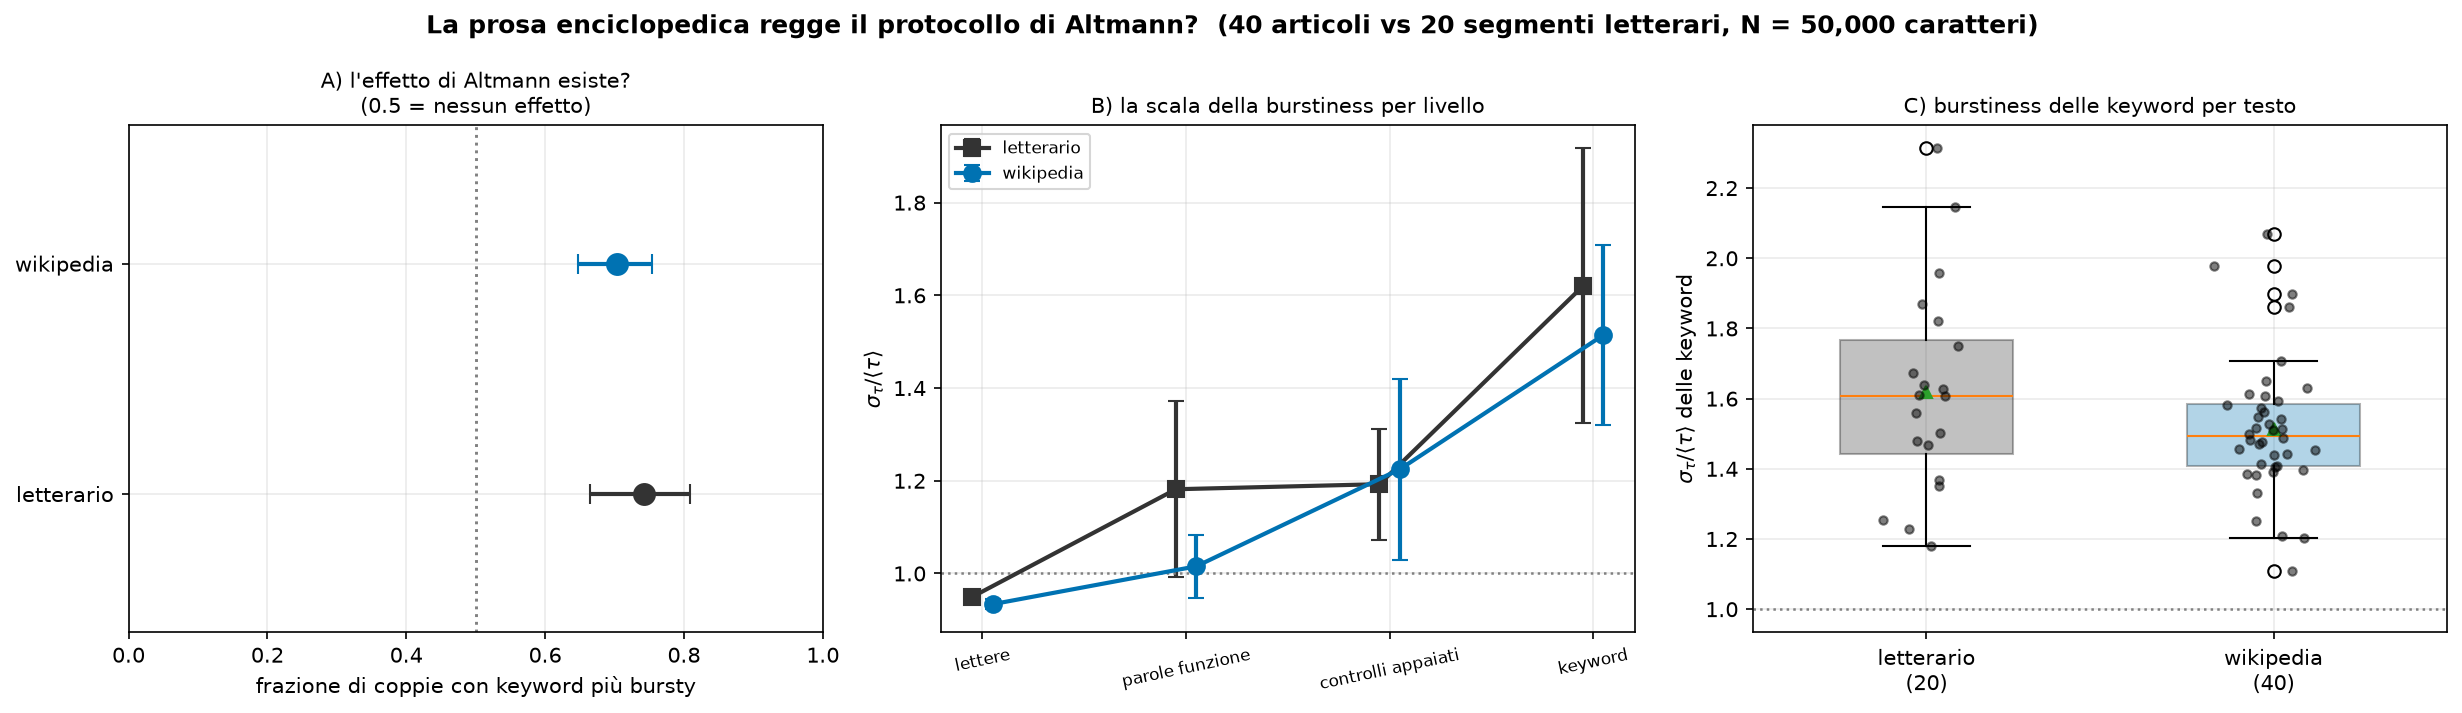
\includegraphics[width=\textwidth]{figure/cap5_wiki_altmann.png}
  \caption{Test di fattibilità del protocollo su prosa enciclopedica, condotto
  su \num{40} voci di Wikipedia e \num{20} segmenti letterari a \num{50000}
  caratteri. A: quota di confronti in cui la parola chiave supera il proprio
  controllo appaiato in frequenza, con intervallo di confidenza al $95\%$; la
  linea punteggiata a $0.5$ è l'assenza di effetto. B: coefficiente di
  variazione degli intervalli ai quattro livelli linguistici. C: distribuzione
  della burstiness delle parole chiave testo per testo. Questa è l'unica figura
  del capitolo costruita su \num{40} voci e \num{50000} caratteri; tutte le
  successive usano \num{39} terne e \num{60000} caratteri.}
  \label{fig:wiki-fattibilita}
\end{figure}

% ---------------------------------------------------------------------
\section{L'effetto nei tre corpora}
\label{sec:tre-corpora}

L'analisi principale confronta Wikipedia, le due versioni di Grokipedia e
l'ancora letteraria su \num{39} terne complete, troncate a \num{60000}
caratteri. La voce esclusa è \emph{Buddhism}, per la ragione riportata nel
§\ref{sec:paternita}: la sua versione v0.1 è ricopiata da Wikipedia, e in un
disegno appaiato un titolo che cade in un corpus deve cadere in tutti.

\paragraph{La finestra su cui l'esponente è stimato.}
L'esponente di correlazione $\hat\gamma$ è ottenuto interpolando
la~\eqref{eq:sigma} nell'intervallo fisso $t \in (100, 2000)$ caratteri.
\cite{altmann2012} adotta invece una regola relativa e ferma la finestra
all'uno per cento della lunghezza del testo. Le due scelte non sono ordinabili
una volta per tutte: applicata ai romanzi interi che quel lavoro analizza la
regola relativa dà un tetto dell'ordine di \num{10000} caratteri, molto più
largo di quello adottato qui; applicata alle finestre da \num{60000} caratteri
di questo capitolo dà $t < 600$, molto più stretto. L'intera catena è stata
ripetuta anche con la seconda. Il
livello medio di $\hat\gamma$ si abbassa di qualche centesimo, sulle parole
chiave da $1.23$ a $1.18$ per Wikipedia e da $1.32$ a $1.22$ per il romanzo,
ma l'ordinamento fra i corpora resta identico a tutti e quattro i livelli. Il
divario appaiato fra Grokipedia attuale e Wikipedia sulle parole chiave passa
da $-0.049$ a $-0.076$, cioè si accentua invece di ridursi, e resta
significativo in entrambi i casi. Le conclusioni di questo capitolo non
dipendono dunque dalla finestra scelta.

\paragraph{Tre modi di leggere il confronto.}
La Figura~\ref{fig:tre-corpora} riporta i tre modi in cui il confronto può
essere letto. Il primo pannello ripete il test del paragrafo precedente sui
quattro corpora: la quota di confronti vinti dalle parole chiave vale
$114/140 = 0.814$ sul romanzo, $189/273 = 0.692$ su Wikipedia,
$195/273 = 0.714$ su Grokipedia v0.1 e $202/273 = 0.740$ su Grokipedia nella
versione attuale. Ripetendo lo stesso test sull'esponente di correlazione
$\hat\gamma$ anziché sulla burstiness, la quota di confronti vinti dalle parole
chiave vale $0.907$ sul romanzo, $0.747$ su Wikipedia, $0.769$ su Grokipedia
v0.1 e $0.791$ su Grokipedia nella versione attuale.
L'effetto esiste ovunque, con tutti e quattro gli
intervalli di confidenza interamente sopra $0.5$, ed è massimo sul romanzo;
fra le due enciclopedie, però, non distingue: i valori di Grokipedia sono anzi
lievemente superiori a quelli di Wikipedia, con intervalli che si sovrappongono.
La domanda a cui questo pannello risponde è se la parola chiave superi il
proprio controllo a frequenza appaiata dentro lo stesso testo, e la
risposta è che ciò accade con la stessa frequenza nei due corpora enciclopedici.
Il deficit di Grokipedia, misurato dai pannelli successivi, non riguarda dunque
l'esistenza del meccanismo ma il livello assoluto della burstiness.

Il secondo pannello mostra il coefficiente di variazione ai quattro livelli e
rende visibile dove la differenza si concentra. Sulle lettere i quattro corpora
sono indistinguibili, tutti compresi fra $0.922$ e $0.950$, e sulle parole
funzione la separazione resta modesta, da $0.967$ a $1.192$. Il divario si apre
ai due livelli lessicali: sui controlli appaiati il romanzo raggiunge $1.262$,
Wikipedia $1.190$ e le due versioni di Grokipedia $1.044$ e $1.055$; sulle
parole chiave rispettivamente $1.789$, $1.536$, $1.387$ e $1.379$. 
Il terzo pannello riporta la stessa quantità testo per testo,
e mostra che la separazione non è l'effetto di pochi articoli anomali: le
distribuzioni di Wikipedia e di Grokipedia si sovrappongono, ma le loro mediane
differiscono di circa $0.25$ e la coda superiore di Wikipedia è più popolata.

\begin{figure}[htbp]
  \centering
  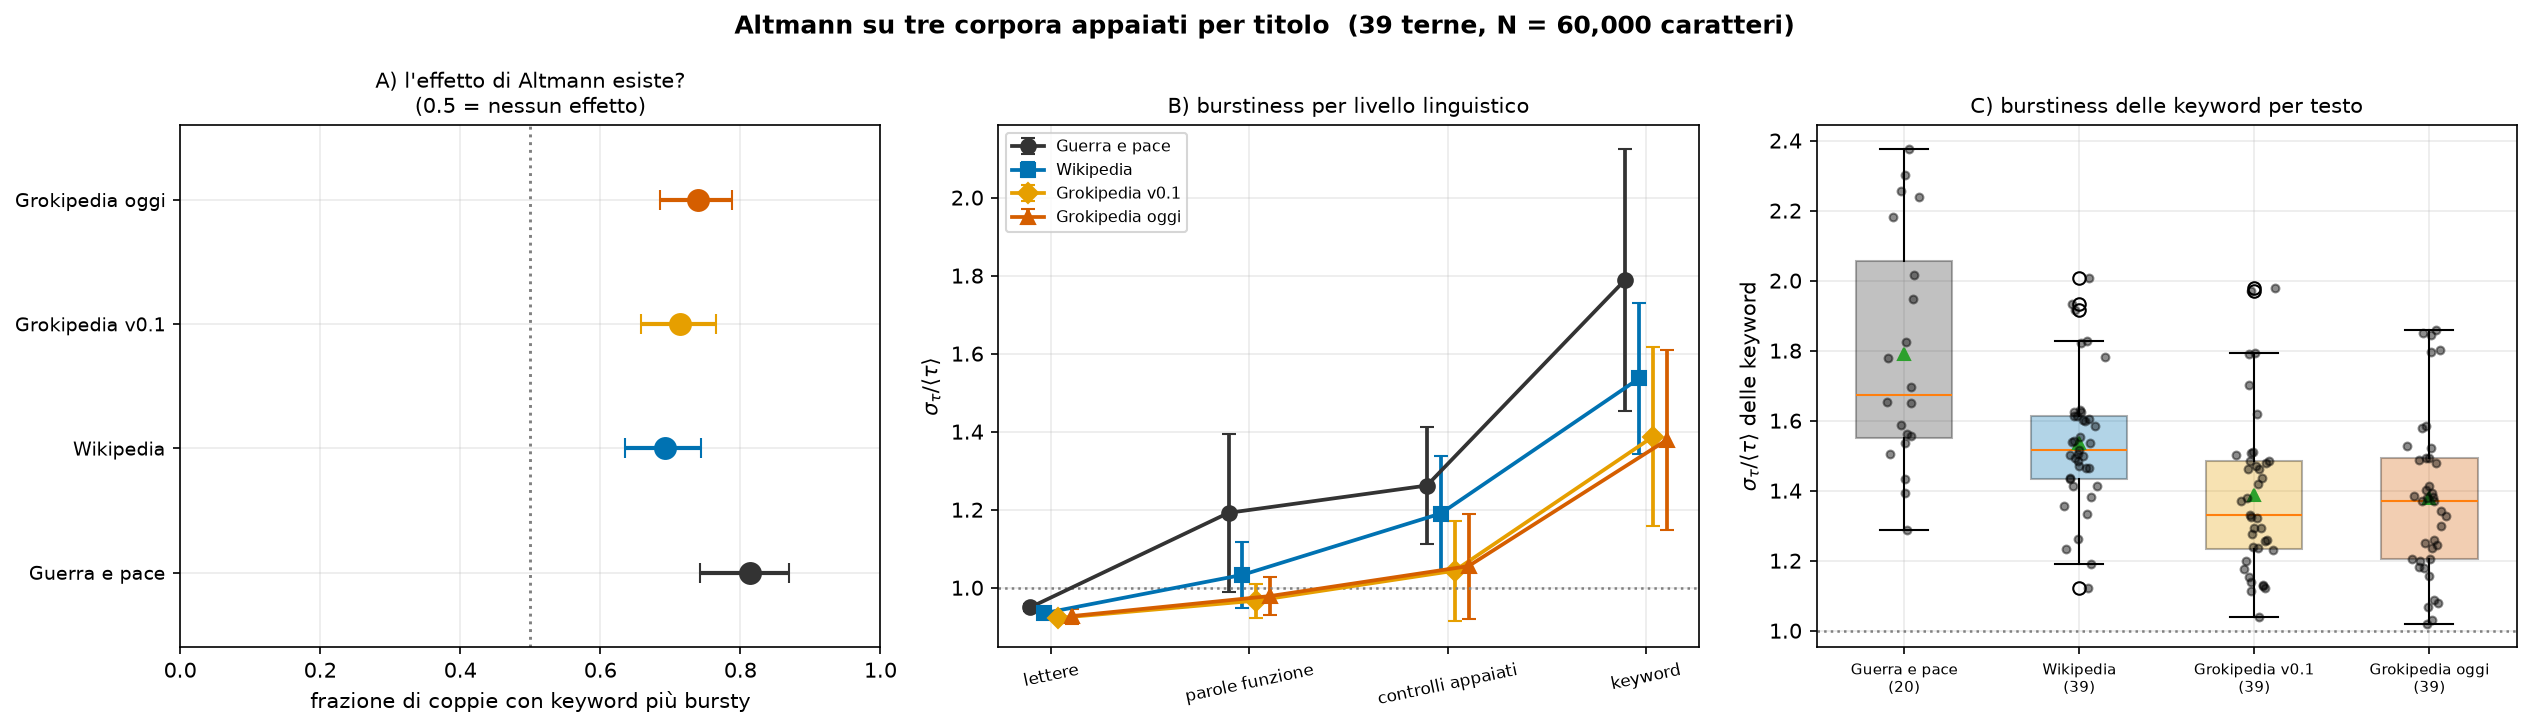
\includegraphics[width=\textwidth]{figure/cap5_tre_corpora.png}
  \caption{Il protocollo di Altmann sui quattro corpora, \num{39} terne
  appaiate per titolo a \num{60000} caratteri. A: quota di confronti vinti dalle
  parole chiave, con intervallo di confidenza al $95\%$. B: coefficiente di
  variazione degli intervalli ai quattro livelli linguistici; le barre sono
  deviazioni standard fra testi. C: burstiness delle parole chiave testo per
  testo, con mediana, quartili e singoli punti sovrapposti. Il numero di testi
  per corpus è indicato sotto ciascuna colonna.}
  \label{fig:tre-corpora}
\end{figure}

\paragraph{L'ancora letteraria è un testo, non un genere.} Il primato del
romanzo sui due livelli lessicali non sopravvive al cambio di testo. Ripetendo
l'intera misura su tre altri romanzi inglesi trattati esattamente come
\emph{Guerra e pace}, cioè \emph{Moby Dick}, \emph{Middlemarch} e \emph{David
Copperfield}, gli stessi impiegati come controllo nel
§\ref{sec:coda-risultati}, sulle parole chiave si ottiene $1.55$, $1.54$ e
$1.63$, cioè valori sostanzialmente pari a quello di Wikipedia e ben al di
sotto dell'$1.79$ di \emph{Guerra e pace}; alle parole funzione si ottiene
$1.03$, $1.08$ e $1.09$, contro l'$1.19$ del romanzo di riferimento e l'$1.03$
di Wikipedia. La distanza fra prosa letteraria e prosa enciclopedica non è
dunque un fatto generale, e l'ancora letteraria di questo capitolo va letta
per ciò che è: un termine di paragone concreto, non la misura di un genere.
Nulla di ciò che segue vi poggia, perché il risultato del capitolo è un
confronto appaiato fra le due enciclopedie, dove il romanzo non entra.

Il null model A1 restituisce un esponente medio di $0.983$ su tutte le celle,
in accordo con l'unità che deve dare per costruzione: la procedura di stima si
comporta come nel §\ref{sec:validazione} anche su questi corpora.

\paragraph{L'analogo della Figura~2 di~\cite{altmann2012}.}
La Figura~\ref{fig:altmann-fig2} riproduce sui quattro corpora la costruzione
con cui~\cite{altmann2012} presenta il proprio risultato principale, e permette
di verificarne l'aderenza riga per riga. Per ogni corpus vengono mostrate una
lettera e una parola di contenuto, ciascuna con la distribuzione cumulata degli
intervalli e con la crescita della varianza del conteggio, accanto alle stesse
curve calcolate sui due null model.

\paragraph{Quale parola mostrare.} La scelta della parola da mostrare pone un
problema che il caso della lettera non ha. Selezionare la parola chiave più
ricorrente del corpus, che è il criterio più immediato, produce oggetti
strutturalmente diversi nei due tipi di prosa: in un romanzo pesca il nome di
un personaggio, presente solo nelle scene in cui il personaggio compare,
mentre in un'enciclopedia pesca il soggetto della voce, che ricorre in quasi
ogni frase. Le due parole finirebbero alle code opposte delle rispettive
distribuzioni di burstiness, al $96$ e al $2$ percentile, e la figura
confronterebbe due casi estremi anziché due casi tipici. La parola mostrata è
quindi quella con $\sigma_\tau/\langle\tau\rangle$ più vicino alla mediana del
proprio corpus, fra quelle con almeno \num{40} occorrenze; il percentile
effettivo è riportato sopra ciascun pannello e sta fra $45$ e $57$ in tutti e
quattro i corpora. Il caso escluso ha però un interesse proprio, ed è ripreso
subito dopo la figura.

\paragraph{Che cosa mostrano le quattro righe.}
Il comportamento è allora quello descritto nel §\ref{sec:origini}, e vale su
tutte e quattro le righe. Sulla lettera la cumulata decade rapidamente e
l'esponente del null model A2 si dispone attorno all'unità, $0.94$ sul romanzo,
$0.90$ su Wikipedia, $0.94$ sulla v0.1 e $1.05$ sulla versione attuale di
Grokipedia, perché a quel livello la burstiness non contribuisce. Lo scarto
massimo da uno vale un decimo, ed è quanto ci si attende su una singola
sequenza: aggregando tutte le \num{2603} sequenze di livello letterale dei
quattro corpora $\hat\gamma_{A2}$ vale fra $0.983$ e $0.990$, con una
dispersione fra sequenze di $0.044$, cosicché i quattro valori della figura
stanno tutti entro due deviazioni standard dall'unità. Un solo caso per corpus
non permette dunque una lettura più fine di così.

Sulla parola di contenuto la cumulata ha coda larga, con
$\sigma_\tau/\langle\tau\rangle$ fra $1.23$ e $1.79$, e $\hat\gamma_{A2}$
resta sopra l'unità e più vicino a $\hat\gamma$ che nel caso della lettera:
$1.36$ contro $1.43$ sul romanzo, $1.09$ contro $1.20$ su Wikipedia, $1.09$
contro $1.23$ sulla v0.1 e $1.11$ contro $1.20$ sulla versione attuale. Una
parte della correlazione passa cioè attraverso la distribuzione degli
intervalli, e la frazione è massima sul romanzo. La figura mostra il
meccanismo su un caso per corpus e non va letta come misura del divario fra
corpora: quella richiede l'aggregato del §\ref{sec:decomposizione}, perché su
una singola parola la differenza fra i due esponenti è dominata dal rumore di
stima. Lo si vede nella riga di Grokipedia attuale, dove sulla lettera
$\hat\gamma = 0.94$ scende sotto $\hat\gamma_{A2} = 1.05$, cosa che
sull'aggregato di quel livello, dove il rumore si media, non accade.

La lettera \emph{e} in \emph{Guerra e pace} dà qui un coefficiente di
variazione pari a $0.85$ contro lo $0.83$ della didascalia della Figura~2
di~\cite{altmann2012}, il che vale come controllo indipendente delle
procedure: la stessa quantità, misurata sullo stesso testo da un codice
diverso, coincide entro due centesimi.

\begin{figure}[htbp]
  \centering
  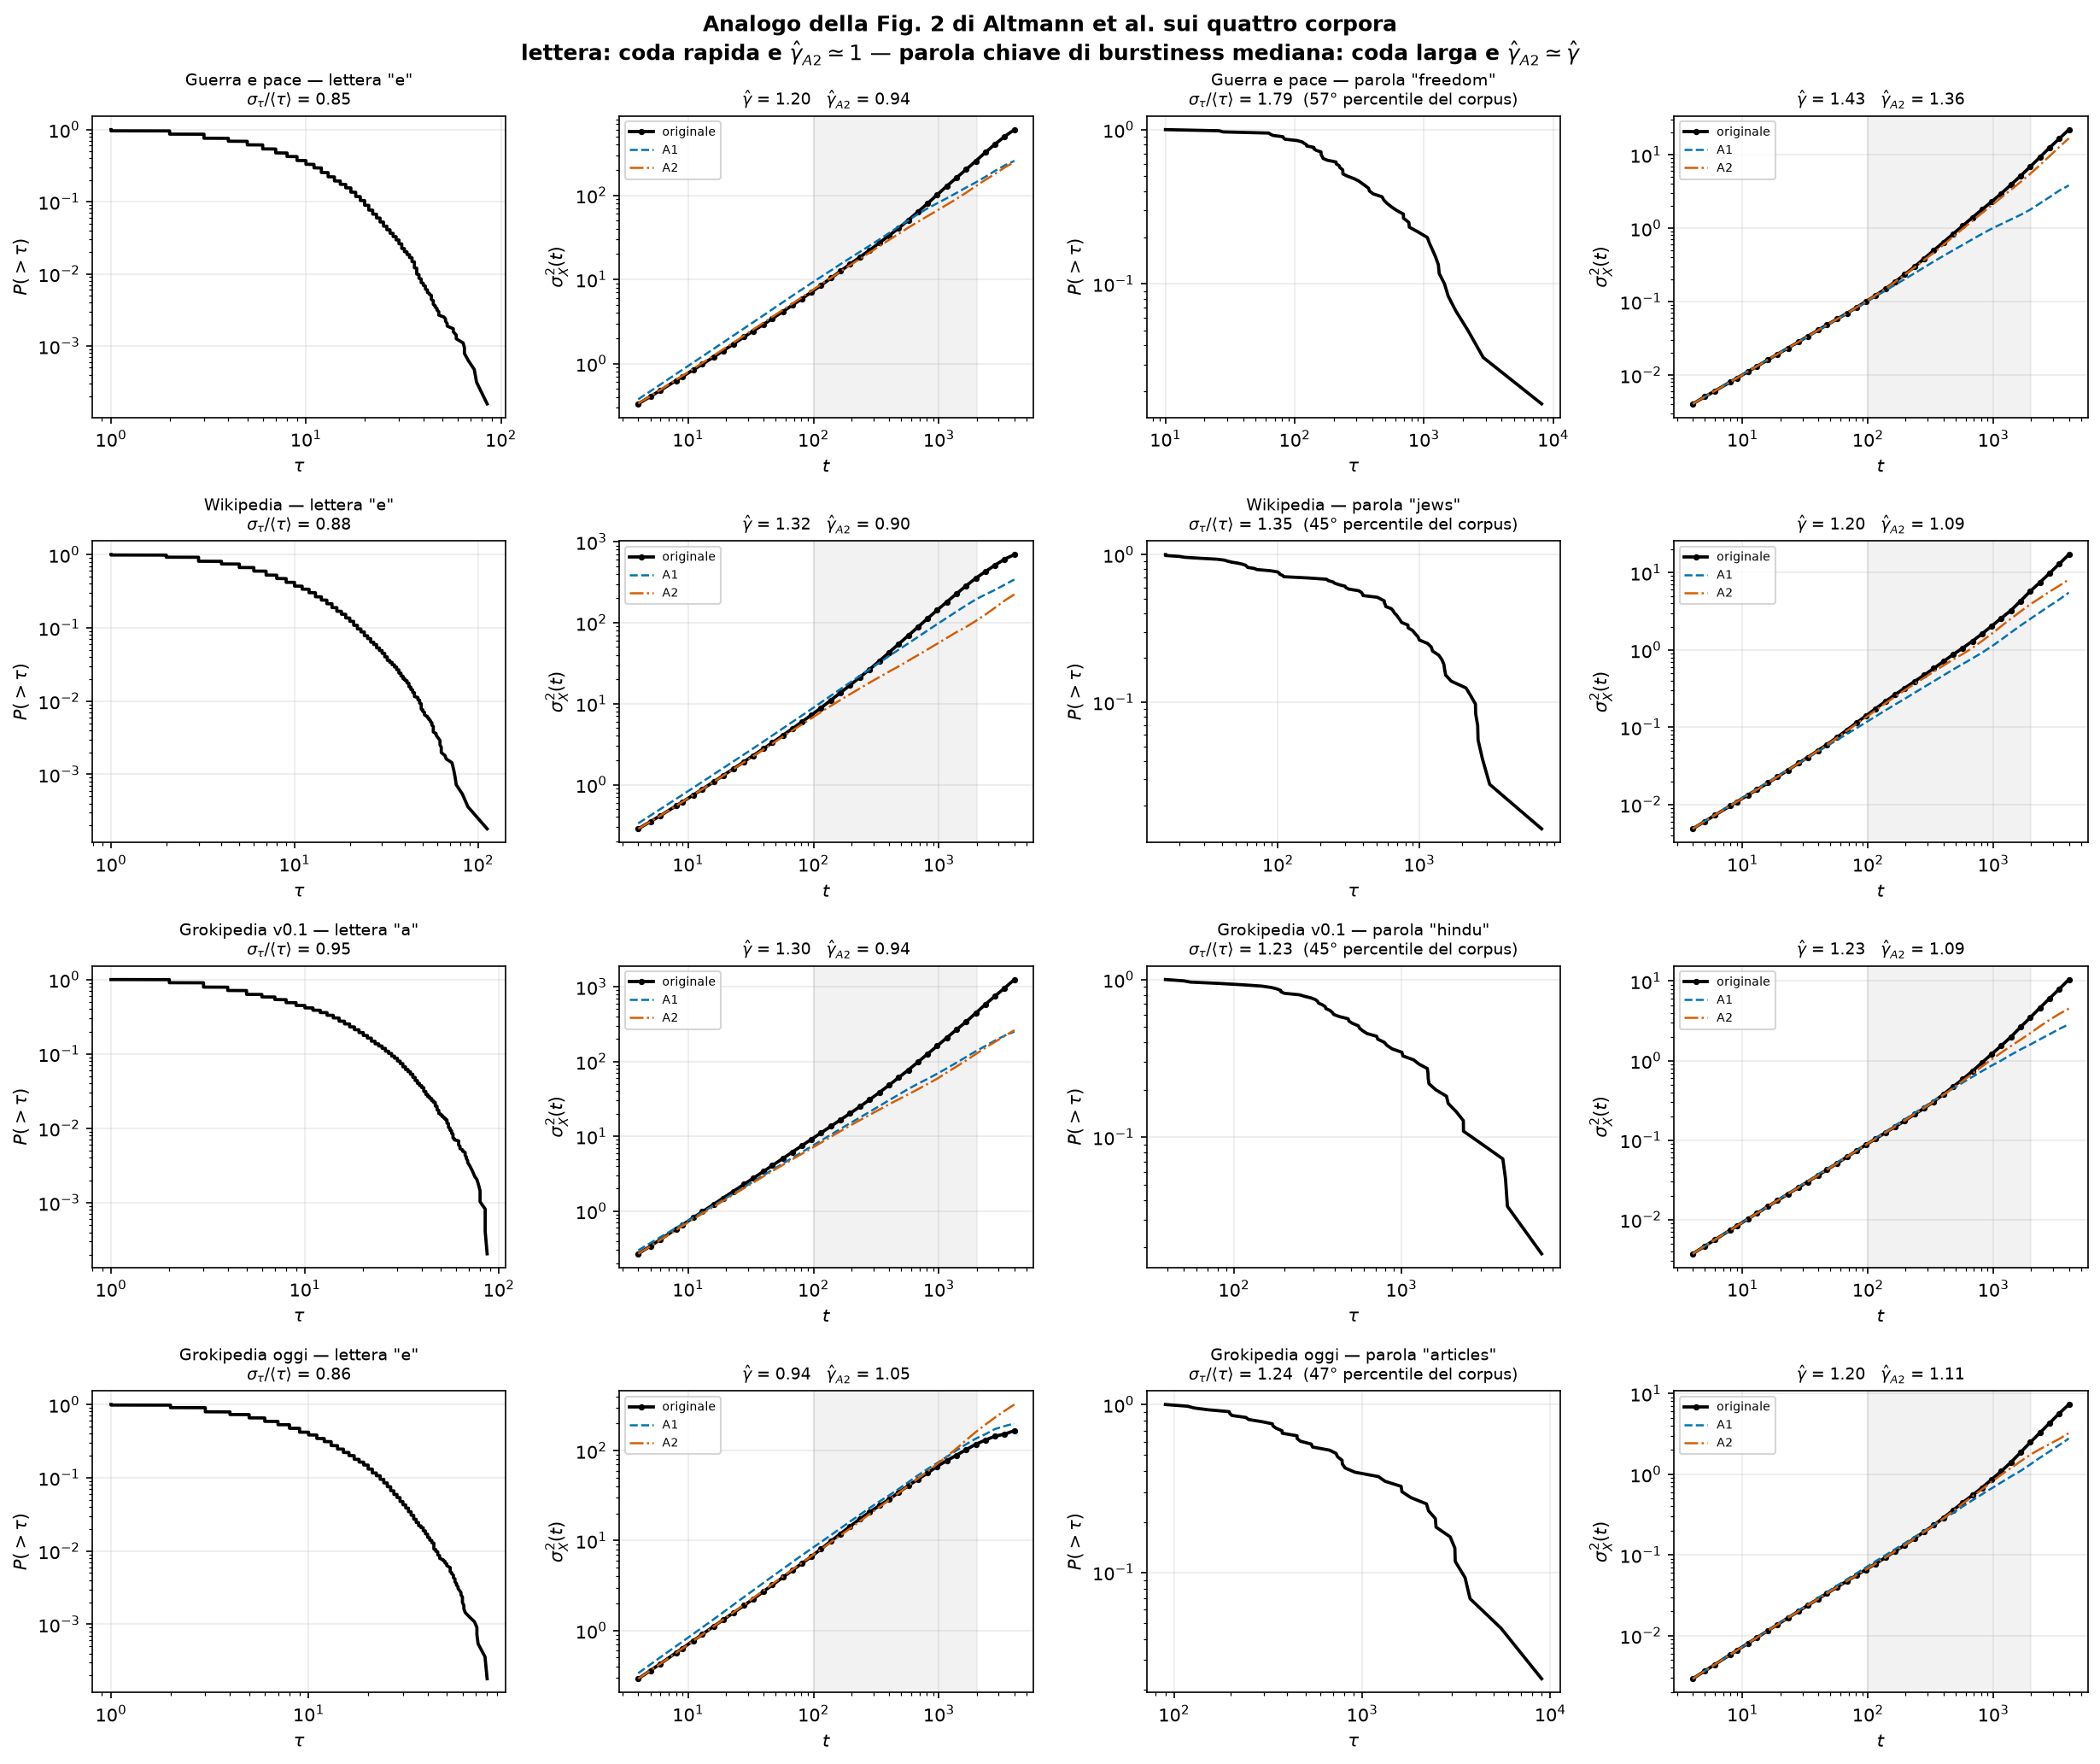
\includegraphics[width=\textwidth]{figure/cap5_altmann_fig2.png}
  \caption{Analogo della Figura~2 di~\cite{altmann2012} sui quattro corpora. Una
  riga per corpus; a sinistra la lettera più frequente del documento, a destra
  la parola chiave di burstiness mediana del corpus fra quelle con almeno
  \num{40} occorrenze, con il suo percentile indicato sopra il pannello. Per
  ciascuna, la distribuzione cumulata degli intervalli $P(>\tau)$ e la crescita
  della varianza del conteggio $\sigma_X^2(t)$, con le curve dei due null model
  del §\ref{sec:null} e la finestra di fit ombreggiata. La lettera ha coda
  rapida e $\hat\gamma_{A2} \simeq 1$; la parola di contenuto ha coda larga e
  $\hat\gamma_{A2}$ prossimo a $\hat\gamma$.}
  \label{fig:altmann-fig2}
\end{figure}

\paragraph{Il soggetto della voce non è una parola di contenuto.}
La parola chiave più ricorrente di un articolo enciclopedico, quella che il
criterio scartato sopra avrebbe selezionato, si comporta in modo opposto a
quello che il §\ref{sec:origini} prevede per il suo livello linguistico. Nella
voce \emph{Alexander the Great} di Wikipedia la parola \emph{alexander} ha
$\sigma_\tau/\langle\tau\rangle = 0.78$; in \emph{Sigmund Freud} di Grokipedia
\emph{freud} ha $0.72$. Sono valori sotto il limite poissoniano, cioè
distribuzioni \emph{più regolari del caso}, mentre la lettera \emph{e} negli
stessi testi dà $0.84$. Il confronto con la lettera non va però fatto sul valore
grezzo. Per un processo casuale in tempo discreto
$\sigma_\tau/\langle\tau\rangle$ non vale esattamente uno, ma tanto meno quanto
più corti sono gli intervalli: il null model A1, applicato alla stessa frequenza
della sequenza osservata, restituisce $0.95$ per la lettera \emph{e}, che ricorre
ogni dieci caratteri, e $1.00$ per una parola chiave, che ricorre ogni
duecento.

\paragraph{Il riferimento casuale dipende dalla frequenza.}
La ragione di quel $0.95$ è che gli intervalli sono numeri interi positivi. Se
le occorrenze sono collocate a caso con probabilità $f$ per carattere, la
distanza fra due consecutive è geometrica, e per la geometrica si ha
$\sigma_\tau/\langle\tau\rangle = \sqrt{1-f}$: il valore tende a uno solo nel
limite di eventi rari. Con $f = 1/10$, la frequenza della lettera \emph{e}, si
ottiene $0.949$; con $f = 1/200$, la frequenza tipica di una parola chiave,
$0.997$. Il valore poissoniano di riferimento non è dunque lo stesso ai due
livelli, ed è più basso proprio dove gli eventi sono più fitti. Confrontare
\emph{alexander} e la lettera \emph{e} sui valori grezzi significherebbe
attribuire alla struttura del testo una differenza che è invece un effetto
della sola frequenza.

Rapportando ciascuna misura al proprio valore casuale l'effetto si toglie, e
resta $0.78$ per \emph{alexander} contro $0.88$ per la lettera: il soggetto
della voce è più regolare di una lettera anche dopo aver tolto l'effetto della
frequenza, e la differenza fra i due, lungi dall'essere prodotta dalla
normalizzazione, ne esce accentuata.

\paragraph{Perché il soggetto si comporta così.}
La ragione è che in prosa enciclopedica il soggetto non è un tema fra altri,
che alterna presenza e assenza lungo il testo, ma il tema unico: compare come soggetto grammaticale di quasi ogni
periodo, e i suoi intervalli ereditano allora la statistica della lunghezza
delle frasi anziché quella dell'alternanza tematica. La verifica è diretta.
Nei sei articoli esaminati il soggetto ricorre una volta ogni $1.4$--$1.7$
frasi, con lo stesso valore in Wikipedia e in Grokipedia. I suoi intervalli sono
quindi lunghezze di frase, e ne ereditano la variabilità: le
lunghezze di frase di quegli articoli hanno
$\sigma_\tau/\langle\tau\rangle$ fra $0.33$ e $0.73$, e il soggetto della voce
si colloca poco sopra, fra $0.54$ e $0.78$, comunque sotto l'unità che
segnerebbe l'assenza di struttura. Per confronto, \emph{natásha} in un segmento
di \emph{Guerra e pace} ricorre una volta ogni $5.1$ frasi e ha
$\sigma_\tau/\langle\tau\rangle = 3.24$: lì la ricorrenza non segue il ritmo del
periodo ma l'alternanza delle scene.

Il soggetto della voce funziona quindi da marcatore sintattico e non semantico,
e la sua ricorrenza è governata dal ritmo del periodo, non dalla persistenza di
un argomento. Non è un difetto della misura ma un tratto del genere
enciclopedico, e va tenuto presente nel confrontare la burstiness lessicale fra
generi diversi: è la ragione per cui la parola mostrata nella
Figura~\ref{fig:altmann-fig2} viene scelta sulla mediana e non sul massimo.

% ---------------------------------------------------------------------
\section{Il divario si apre al livello lessicale}
\label{sec:appaiato}

L'appaiamento per titolo permette un test più stringente del confronto fra
medie. Confrontare la media di Wikipedia con quella di Grokipedia lascia
aperta l'obiezione che le due medie siano calcolate su argomenti diversi, e
che la differenza rifletta il contenuto anziché la scrittura. Il test appaiato
la chiude: per ciascuna delle \num{39} voci, che nei due corpora tratta lo
stesso argomento, si calcola la differenza fra il valore di Grokipedia e
quello di Wikipedia, e si verifica con il test dei ranghi segnati di Wilcoxon
che la mediana di quelle \num{39} differenze sia diversa da zero. Il test è
non parametrico, quindi non assume che le differenze siano distribuite
normalmente, assunzione che con \num{39} osservazioni e distribuzioni
asimmetriche non sarebbe difendibile.

Il test dà, per la versione attuale di Grokipedia,
$-0.167$ sulle parole chiave e $-0.010$ sulle lettere; ai due livelli intermedi
le differenze valgono $-0.037$ per le parole funzione e $-0.157$ per i controlli
appaiati, tutte con significatività inferiore a $10^{-2}$. La versione v0.1 dà
$-0.012$, $-0.039$, $-0.116$ e $-0.133$.

I quattro numeri vanno letti come una scala. Alle lettere Grokipedia e
Wikipedia distano un centesimo di unità di burstiness, cioè circa l'uno per
cento del valore misurato: a quel livello i due corpora sono, in pratica, lo
stesso testo. Alle parole funzione la distanza quadruplica, ma resta piccola in
termini relativi. Ai due livelli lessicali passa a circa sedici centesimi, oltre
un decimo del valore misurato e più di un ordine di grandezza sopra il livello
delle lettere.

La scala ha però un solo gradino, non tre. La differenza fra i livelli
sub-lessicali e quelli lessicali è netta; quella fra i due livelli lessicali non
esiste: $-0.157$ sui controlli a frequenza appaiata contro $-0.167$ sulle parole
chiave sono lo stesso numero. Il testo generato non perde dunque le parole di
contenuto più di quanto perda le altre parole della stessa frequenza. Ciò che i
dati sostengono è che riproduca le regolarità dei livelli bassi e abbassi
uniformemente la burstiness a livello di parola, non che perda selettivamente la
persistenza tematica.

\paragraph{Il divario alla lunghezza di controllo.}
\label{sec:robustezza-neff}
L'intera catena è stata ripetuta a $N_{\mathrm{eff}} = \num{80000}$ caratteri,
lunghezza a cui sopravvivono \num{35} delle \num{39} terne; per isolare
l'effetto della finestra, i valori a \num{60000} sono ricalcolati sulle stesse
\num{35}. Alle lettere e alle parole funzione il divario appaiato è stabile, da
$-0.010$ a $-0.011$ e da $-0.037$ a $-0.045$; ai due livelli lessicali si separa
in direzioni opposte, con i controlli appaiati da $-0.164$ a $-0.195$ e le parole
chiave da $-0.167$ a $-0.130$, quest'ultima con significatività che scende a
$p = 0.027$. Alla lunghezza maggiore il divario sulle parole chiave è dunque
\emph{minore} di quello sui controlli appaiati. Ciò che risulta robusto è il
salto dal livello sub-lessicale a quello lessicale; l'ulteriore crescita fino
alle parole chiave non lo è. Anche l'esponente di coda è instabile fra le due
lunghezze, da $2.19$ a $2.50$ su Grokipedia e da $2.37$ a $2.25$ su Wikipedia,
coerentemente con l'avvertenza del §\ref{sec:coda-risultati}.

La Figura~\ref{fig:altmann-fig3} riporta le stesse sequenze nel piano che
\cite{altmann2012} usa per la propria Figura~3: la burstiness in ascissa e
l'esponente di correlazione in ordinata, un punto per sequenza, con un simbolo
diverso per livello linguistico. La gerarchia vi si legge come una disposizione
spaziale: le lettere, gli spazi e le vocali si addensano in una colonna stretta
attorno a $\sigma_\tau/\langle\tau\rangle \simeq 0.5$, le parole funzione e i
controlli appaiati occupano la regione centrale, le parole chiave si spingono a
destra e in alto. È la stessa gerarchia dei paragrafi precedenti, vista tutta
insieme invece che un livello alla volta.

Il piano rende però visibile anche una proprietà che i confronti per livello
non mostrano, e che è l'osservazione centrale di quel lavoro: l'angolo in
basso a destra è vuoto. Non esistono, cioè, sequenze molto \emph{bursty} e
insieme poco correlate. Sui quattro corpora di questa tesi la regolarità si
quantifica così: delle $451$ sequenze con $\sigma_\tau/\langle\tau\rangle >
1.5$, soltanto $17$, il $3.8\%$, hanno $\hat\gamma < 1.1$, e fra quelle con
burstiness superiore a $2$ l'esponente non scende mai sotto $1.05$. L'angolo
opposto, invece, è popolato: delle $3500$ sequenze sotto il valore poissoniano
$\sigma_\tau/\langle\tau\rangle = 1$, il $15.9\%$ ha $\hat\gamma > 1.2$.

L'asimmetria fra i due angoli è la firma di una relazione a senso unico. La
burstiness produce correlazione, come mostra la~\eqref{eq:eq4}, e una sequenza
con vuoti lunghi non può quindi risultare scorrelata; il viceversa non vale,
perché la correlazione può venire anche dall'ordine degli intervalli e
manifestarsi senza alcuna coda pesante. La correlazione di rango fra le due
quantità è positiva e significativa in tutti e quattro i corpora, da $+0.22$ su
Wikipedia a $+0.36$ sul romanzo. Il meccanismo descritto in~\cite{altmann2012}
sui romanzi si ritrova dunque identico nella prosa enciclopedica e in quella
generata, ed è un risultato indipendente dal divario misurato sopra: riguarda
come le due grandezze si legano fra loro, non quanto valgano.

\begin{figure}[htbp]
  \centering
  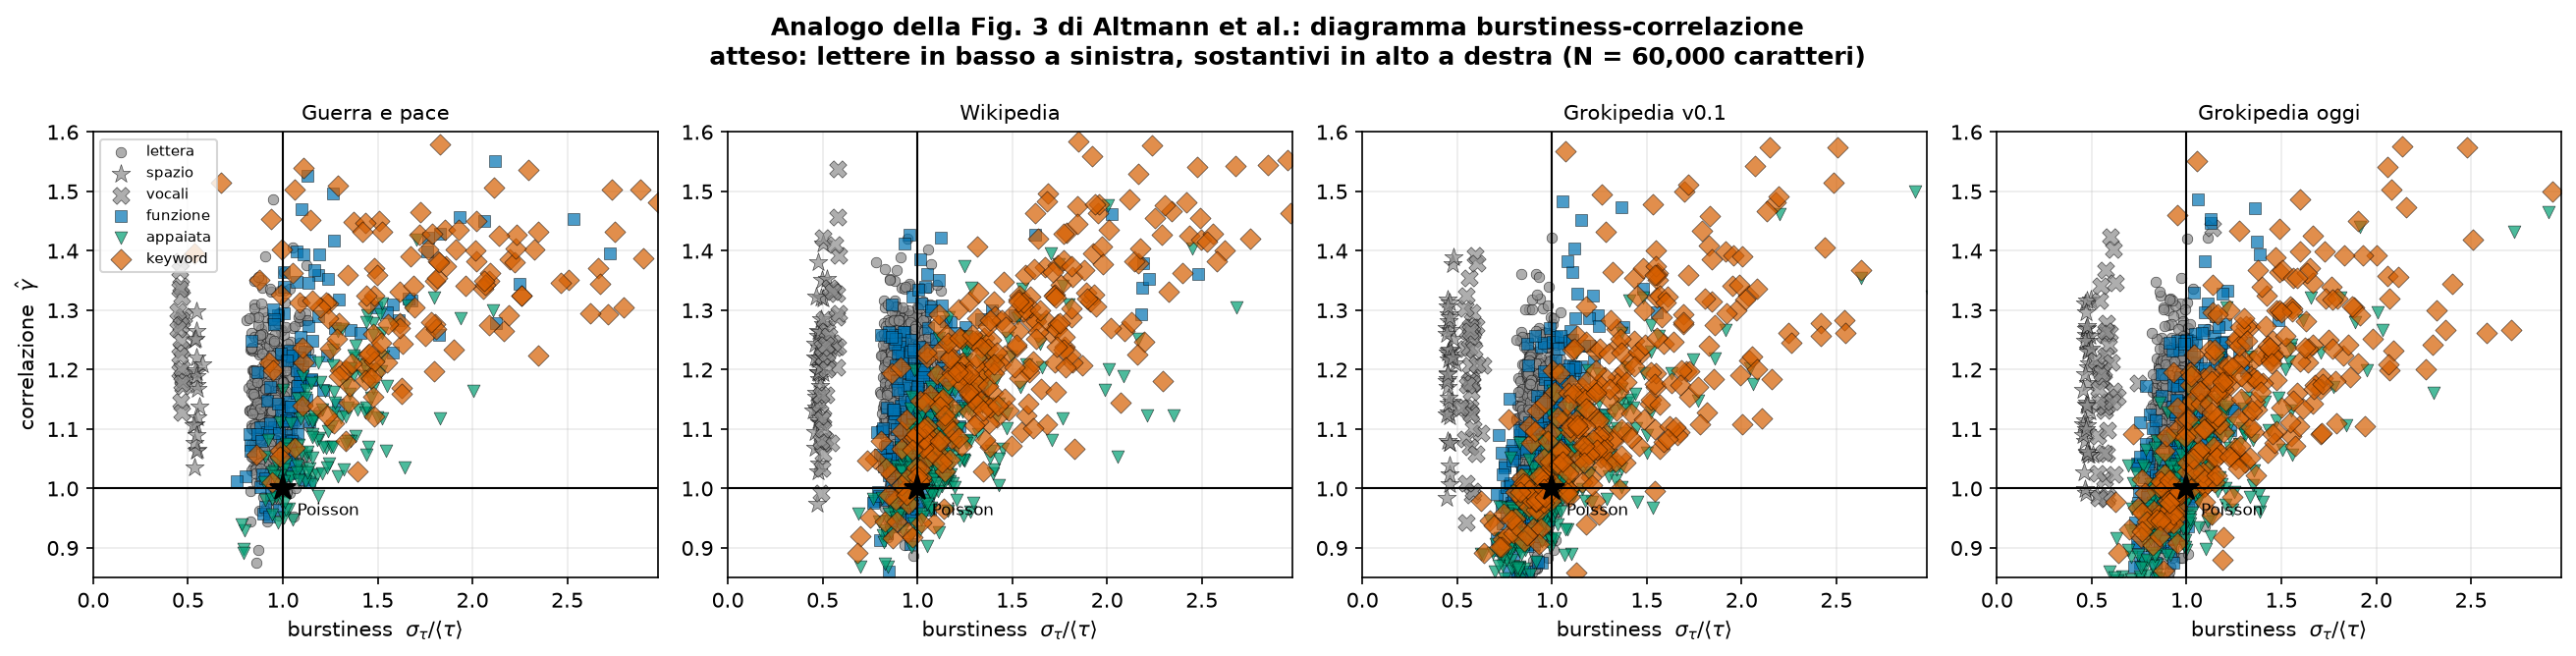
\includegraphics[width=\textwidth]{figure/cap5_altmann_fig3.png}
  \caption{Analogo della Figura~3 di~\cite{altmann2012}: diagramma
  burstiness--correlazione sui quattro corpora, un punto per sequenza. Oltre ai
  quattro livelli usati nel resto del capitolo sono riportati i due livelli
  sub-lessicali tenuti come diagnostica, gli spazi e le vocali. Le linee nere
  segnano il processo di Poisson,
  $\sigma_\tau/\langle\tau\rangle = 1$ e $\hat\gamma = 1$. L'angolo in basso a
  destra è praticamente vuoto in tutti e quattro i corpora: sequenze molto
  bursty e insieme poco correlate non si osservano.}
  \label{fig:altmann-fig3}
\end{figure}

\paragraph{I due quadranti che restano.} La lettura del piano fatta finora
riguarda la diagonale: l'angolo in basso a destra vuoto e quello in alto a
sinistra popolato. Gli altri due separano però i corpora meglio di qualunque
media, e la Figura~\ref{fig:quadranti} li riporta separatamente. Fra le parole
chiave, l'angolo in alto a destra è la posizione canonica
di~\cite{altmann2012}, quella in cui la sequenza è insieme bursty e correlata.
Vi ricade il $91.4\%$ delle sequenze di \emph{Guerra e pace} e l'$87.5\%$ di
quelle di Wikipedia, ma solo il $74.0\%$ di Grokipedia v0.1 e il $77.3\%$
della versione attuale. La differenza finisce quasi interamente nell'angolo
opposto, in basso a sinistra, dove la parola è più regolare di un processo di
Poisson e insieme priva di correlazione a lungo raggio: $0\%$ sul romanzo,
$5.1\%$ su Wikipedia, $15.4\%$ su Grokipedia v0.1 e $14.3\%$ sulla versione
attuale. Una parola chiave generata su sette si trova dunque nell'angolo
opposto a quello canonico, contro una su venti in Wikipedia. Il test appaiato
sulle \num{39} voci conferma che non è un effetto di composizione del
campione: la quota di parole chiave in basso a sinistra cresce in $21$ e $22$
voci su $39$, con differenza mediana $+0.143$ e $p < 10^{-3}$ per entrambe le
versioni.

Due controlli escludono le spiegazioni strumentali. Il null model A1
restituisce $\hat\gamma = 0.983$ in tutti e quattro i corpora, identico alla
terza cifra, quindi la soglia $\hat\gamma = 1$ non è tarata diversamente da un
corpus all'altro; il valore calibrato non è però esattamente uno, cosicché la
soglia è lievemente generosa verso il lato correlato, allo stesso modo per
tutti. E la quota di parole in basso a sinistra resta più alta in Grokipedia
dentro quattro fasce di frequenza su cinque, da $0.159$ contro $0.050$ per le
parole con $26$--$35$ occorrenze a $0.303$ contro $0.076$ per quelle con più di
$80$. Fa eccezione la fascia più bassa, $15$--$25$ occorrenze, dove il rapporto
si inverte, $0.065$ contro $0.200$; lì però le parole chiave di Wikipedia sono
dieci in tutto e la quota è stimata su di esse. Il divario non dipende quindi
dal fatto che le parole chiave di Wikipedia siano più frequenti, salvo nella
fascia in cui il confronto ha meno appoggio.

Guardare dentro il quadrante non rivela più un gruppo omogeneo. Separando le
parole che compaiono nel titolo della voce dalle altre, le $14$ di Wikipedia si
dividono a metà, e le $39$ di Grokipedia si dividono in $18$ soggetti di voce e
$21$ altre parole, prevalentemente aggettivi generici: \emph{economic} in cinque
voci, \emph{military} in tre, \emph{urban} in due. Sono concentrazioni modeste,
e soprattutto non sono più quelle che la lista di parole funzione originaria
lasciava passare: con quella lista, il quadrante conteneva \emph{like} in dodici
voci, \emph{amid} in nove e \emph{including} in sei, cioè i connettivi che
costituiscono il vizio stilistico più evidente del testo generato. Quei termini
sono ora classificati come parole funzione, che è ciò che sono, e il
§\ref{sec:effetto-stoplist} misura quanto la loro presenza fra le parole chiave
alterasse i risultati.

\begin{figure}[htbp]
  \centering
  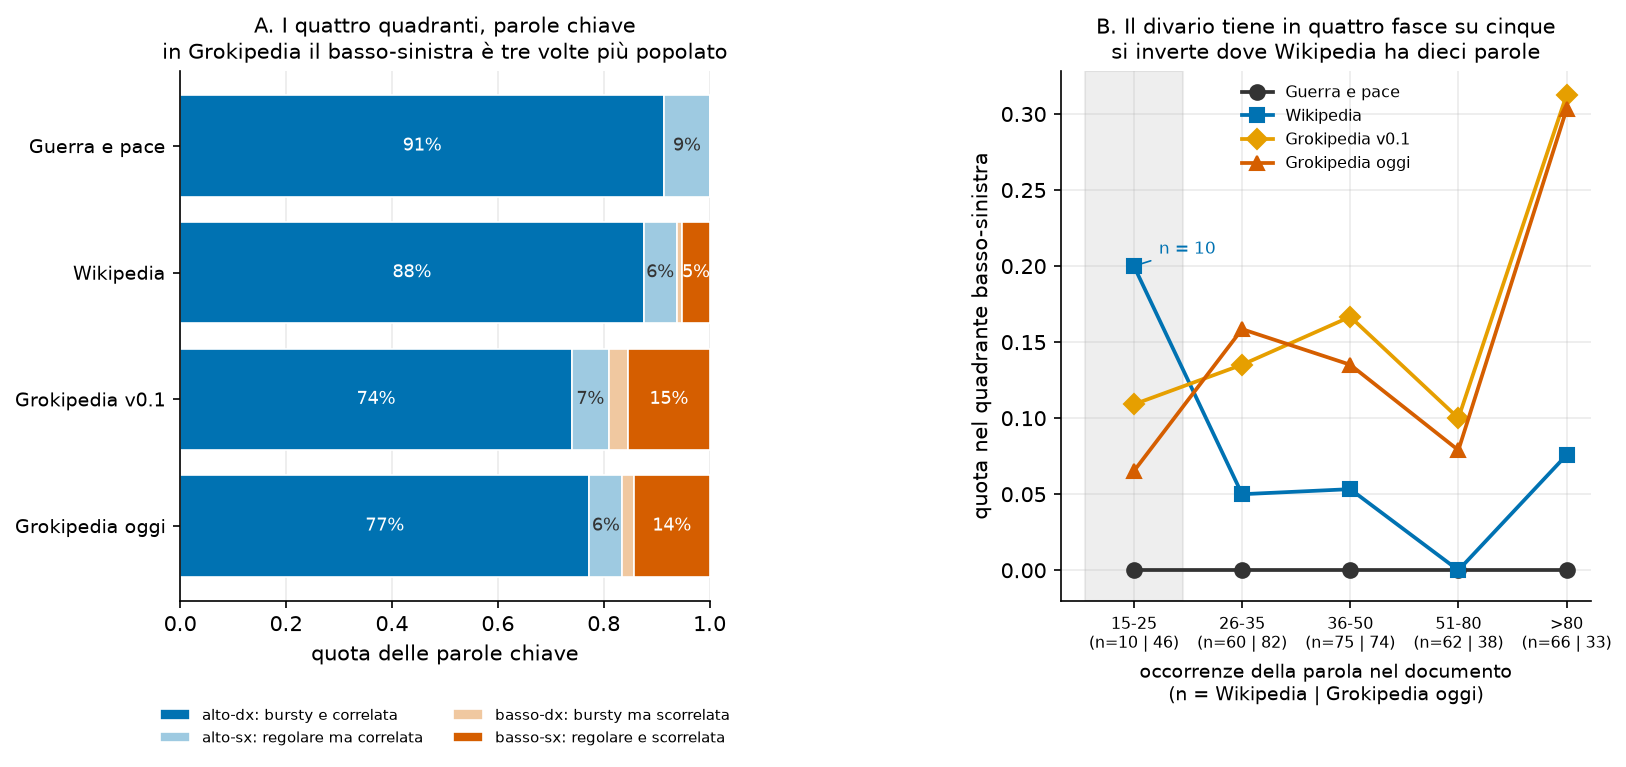
\includegraphics[width=\textwidth]{figure/cap5_quadranti.png}
  \caption{Lettura per quadranti del piano della
  Figura~\ref{fig:altmann-fig3}, sulle sole parole chiave. A: composizione per
  quadrante, un corpus per riga; le quote sotto il $5\%$ non sono etichettate. B:
  quota di parole chiave nel quadrante in basso a sinistra, separando le parole
  per numero di occorrenze nel documento; sotto ciascuna fascia è indicato
  quante parole chiave vi cadono in Wikipedia e in Grokipedia. Il divario tiene
  in quattro fasce su cinque e si inverte nella più bassa, dove Wikipedia ne ha
  dieci in tutto e la fascia è ombreggiata per segnalarlo.}
  \label{fig:quadranti}
\end{figure}

\paragraph{Un effetto di scala da neutralizzare.} Le voci di Grokipedia hanno
frasi sensibilmente
più lunghe di quelle di Wikipedia: $4.38$ frasi ogni mille caratteri contro
$6.92$. Poiché in questo capitolo il tempo è contato in caratteri, la scala
degli intervalli $\tau$ non è la stessa nei due corpora, e un testo con frasi
più lunghe tende ad avere intervalli più lunghi anche a parità di struttura
tematica. Il coefficiente di variazione è un rapporto e non risente di una
dilatazione uniforme dell'asse, ma la dilatazione qui non è uniforme, perché
agisce solo sui livelli definiti su unità linguistiche. Il
§\ref{sec:entropia-intervalli} introduce la misura che elimina il problema;
fino a quel punto il divario va considerato provvisorio.

Il riferimento letterario, infine, non è appaiato per argomento con nessuno dei
tre corpora enciclopedici: entra nei confronti come livello medio e non nei test
appaiati.

% ---------------------------------------------------------------------
\section{Quale meccanismo genera la correlazione}
\label{sec:decomposizione}

Sapere che un testo ha correlazioni a lungo raggio non dice da dove esse
vengano. Il §\ref{sec:null} ha introdotto i due null model che separano le due
origini possibili e la quota di burstiness $q$ della~\eqref{eq:quota}, che vale
circa uno quando la correlazione è interamente spiegata dalla distribuzione
degli intervalli, e circa zero quando è invece l'ordine in cui le occorrenze si
susseguono a produrla.

Il primo pannello della Figura~\ref{fig:decomposizione} riporta $q$ ai quattro
livelli. Sulle lettere il valore è negativo in tutti e quattro i corpora, da
$-0.06$ su Wikipedia a $-0.19$ su Grokipedia v0.1: le lettere sono correlate,
come mostra il $\hat\gamma$ maggiore di uno, ma non sono \emph{bursty}, e la
correlazione viene interamente dall'ordine. Sulle parole chiave il valore sale a
$0.89$ sul romanzo, $0.77$ su Wikipedia, $0.70$ sulla v0.1 e $0.74$ sulla
versione attuale di Grokipedia: qui quasi tutta la correlazione è già contenuta nella
distribuzione degli intervalli. I due livelli intermedi interpolano fra i due
regimi in modo ordinato.

La dissociazione fra il livello dei caratteri e quello del contenuto, che
in~\cite{altmann2012} è osservata su romanzi, si ritrova quindi identica nella
prosa enciclopedica e anche nella prosa generata. Il secondo pannello mostra la
stessa cosa in termini di esponenti: le curve piene sono $\hat\gamma$ e quelle
tratteggiate $\hat\gamma_{A2}$, e la distanza verticale fra le due è il
contributo dell'ordine delle occorrenze. Sulle lettere le due curve sono
separate e la tratteggiata sta all'unità; sulle parole chiave si avvicinano e
salgono insieme.

I valori dei tre corpora enciclopedici sono però troppo vicini perché la
differenza sia interpretabile: fra Wikipedia e Grokipedia vale $0.03$ alla
lunghezza di lavoro e cambia segno a quella di controllo del
§\ref{sec:robustezza-neff}. I dati non consentono quindi di attribuire ai due
corpora un'origine diversa della correlazione, ma soltanto un'intensità diversa.

Sulla riga dei controlli appaiati per Grokipedia, infine, la quota è stimabile
solo su $6$ documenti su $39$ per la versione v0.1 e su $8$ per quella
attuale. La ragione non è un difetto della stima ma la grandezza stessa: $q$
ha $\hat\gamma - 1$ al denominatore, e viene calcolata soltanto dove quel
denominatore supera $0.05$, perché sotto quella soglia il rapporto è dominato
dall'errore. A quel livello i documenti di Grokipedia hanno $\hat\gamma$
mediano pari a $1.003$ per la v0.1 e $1.015$ per la versione attuale, contro
$1.091$ di Wikipedia: le loro sequenze di controllo sono essenzialmente
scorrelate, e non c'è alcuna correlazione da decomporre nelle due origini.
L'esclusione è quindi essa stessa un dato, perché è il livello in cui il testo
generato si avvicina di più al caso, ma il valore di $q$ che sopravvive sui
pochi documenti restanti riguarda proprio quelli in cui una correlazione c'è,
e non va letto come una misura del corpus.

\begin{figure}[htbp]
  \centering
  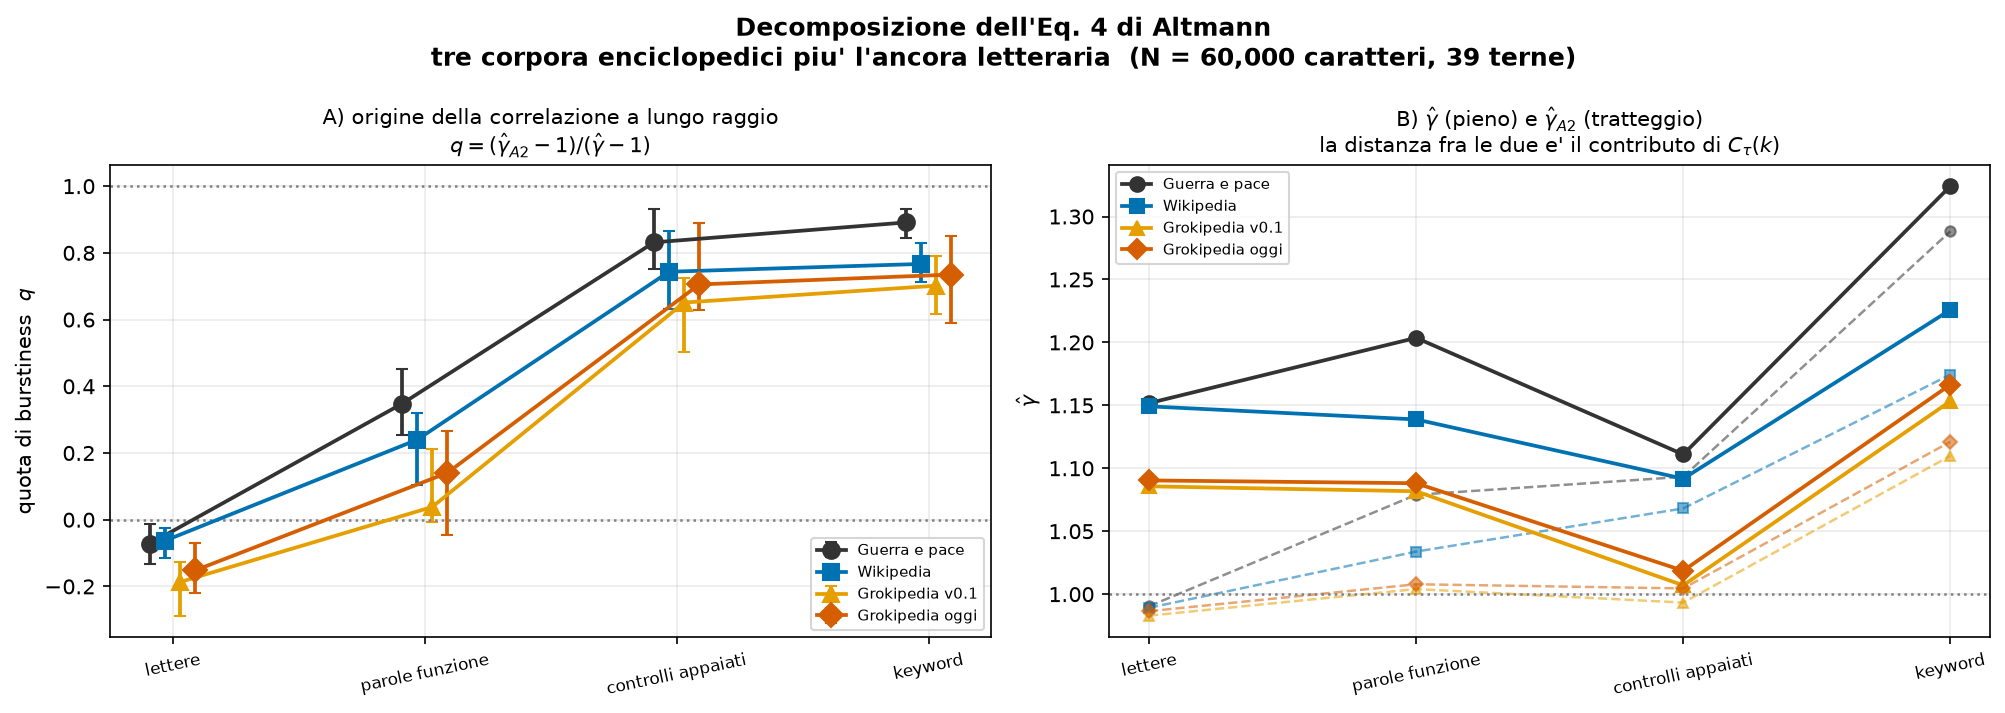
\includegraphics[width=\textwidth]{figure/cap5_decomposizione_eq4.png}
  \caption{Decomposizione della correlazione nelle sue due origini. A: quota
  $q$ della~\eqref{eq:quota} ai quattro livelli linguistici, con intervalli di
  confidenza; $q \simeq 0$ indica correlazione dovuta all'ordine delle
  occorrenze, $q \simeq 1$ correlazione dovuta alla distribuzione degli
  intervalli. B: esponente $\hat\gamma$ (linea piena) e $\hat\gamma_{A2}$
  (tratteggiata) agli stessi livelli; la distanza fra le due curve è il
  contributo della correlazione fra intervalli successivi.}
  \label{fig:decomposizione}
\end{figure}

% ---------------------------------------------------------------------
\section{La coda della distribuzione degli intervalli}
\label{sec:coda-risultati}

Il §\ref{sec:coda} ha osservato che la relazione fra esponente di coda e
esponente di correlazione, nella forma in cui compare in~\cite{altmann2012},
presuppone una distribuzione degli intervalli di cui la coda non viene misurata
ma assunta. Qui la coda viene stimata direttamente, adottando il modello
troncato
\begin{equation}
  p(\tau) \;\sim\; \tau^{-\mu}\,e^{-\tau/\tau_c}
  \label{eq:coda-troncata}
\end{equation}
e determinando $\mu$ e $\tau_c$ per massima verosimiglianza, con intervalli di
confidenza di profilo.

L'analisi della coda comprende, oltre ai quattro livelli usati nel resto del
capitolo, due livelli sub-lessicali aggiuntivi tenuti come diagnostica, le
vocali e gli spazi, per un totale di ventiquattro celle. Il primo risultato
riguarda la forma stessa della distribuzione: il confronto di verosimiglianza
fra la~\eqref{eq:coda-troncata} e una legge di potenza pura rifiuta
quest'ultima in tutte e ventiquattro, con significatività numericamente
indistinguibile da zero. La coda esiste, ma è tagliata.

Il primo pannello della Figura~\ref{fig:coda} riporta $\mu$ ai quattro livelli.
La banda verde segna la regione $2 < \mu < 3$ entro cui la~\eqref{eq:eq8} è
derivata assumendo una legge di potenza pura. Che le stime vi cadano dentro o
fuori non dice nulla sulla convergenza dei momenti: nella
~\eqref{eq:coda-troncata} il taglio li rende finiti per qualunque $\mu$, e il
rifiuto della potenza pura in tutte e ventiquattro le celle toglie il
presupposto sotto cui la banda avrebbe quel significato. Resta un riferimento
utile perché è la regione in cui il paper colloca il proprio valore assunto.
I simboli grigi segnalano le celle in cui il fit degenera in un
esponenziale puro e $\mu$ non è interpretabile, e le linee di collegamento le
saltano. Sono sette celle su sedici: tutti e quattro i corpora sul livello delle
lettere, e i tre corpora enciclopedici su quello delle parole funzione.

Alle parole funzione il romanzo è l'unico dei quattro il cui fit non degenera,
con $\tau_c = 5.3$ contro $1.7$--$1.9$: le sue parole funzione conservano un
tratto di coda a legge di potenza che negli altri tre corpora non esiste, e a
quel livello il coefficiente di variazione dà lo stesso quadro, $1.19$ contro
valori fra $0.97$ e $1.03$ indistinguibili da un processo di Poisson.

Sarebbe naturale leggerlo come una differenza di genere, e il controllo non lo
conferma. Ripetendo la stessa procedura sui tre romanzi inglesi impiegati come
controllo in questo capitolo, il fit sulle parole funzione degenera su
\emph{Moby Dick} ($\tau_c = 1.7$, esattamente il valore dei corpora
enciclopedici) e su \emph{David Copperfield} ($\tau_c = 2.8$), e sopravvive per
poco su \emph{Middlemarch} ($\tau_c = 3.2$); il coefficiente di variazione dà
$1.03$, $1.09$ e $1.08$, cioè valori compresi fra Wikipedia e
\emph{Guerra e pace} e nel primo caso identici a quelli enciclopedici. A questo
livello l'eccezione è quindi del testo e non del genere, come il
§\ref{sec:tre-corpora} osserva anche sul livello delle parole chiave. Il confronto fra i quattro
corpora resta perciò leggibile soltanto sulle parole chiave, dove i valori
stanno fra $1.76$ e $2.37$; sui controlli appaiati tutti e quattro i fit sono al
limite della degenerazione e gli intervalli di confidenza superano l'unità di
ampiezza.

Il confronto con~\cite{altmann2012} chiude qui un cerchio. In quel lavoro $\mu$
non viene stimato ma assunto: per costruire il limite inferiore di $\hat\gamma$
della propria Figura~3 gli autori adottano il valore $\mu = 2.4$. La stima
diretta condotta qui lo colloca dentro l'intervallo di confidenza di tutti e tre
i corpora enciclopedici, e a tre centesimi dal valore centrale di Wikipedia. Il
parametro che quel lavoro doveva postulare risulta dunque misurabile, e il
valore postulato corretto. Il confronto è legittimo perché $\mu$ designa in
entrambi i casi la pendenza della coda nella regione in cui la legge di potenza
vale; ciò che cambia è che qui quella regione è delimitata da un $\tau_c$
stimato anziché estesa all'infinito, e il capoverso seguente misura quanto la
differenza di modello sposti il numero.

Il corpus letterario fa eccezione, con $\mu = 1.76$ e intervallo di confidenza
$[1.40, 2.08]$, e su questo servono due precisazioni, perché il valore cade
sotto la banda $2 < \mu < 3$ entro cui la~\eqref{eq:eq8} è derivata. La prima
è che non è una particolarità di \emph{Guerra e pace}: ripetendo l'intera
procedura su tre altri romanzi inglesi, segmentati e misurati allo stesso
modo, si ottiene $1.51$ su \emph{Moby Dick}, $2.10$ su \emph{Middlemarch} e
$1.96$ su \emph{David Copperfield}, tutti sotto il valore di Wikipedia a ogni
quantile di $x_{\min}$ dall'ottantesimo in su. È un tratto della prosa
letteraria, non del testo scelto, ed è lo stesso fatto che il coefficiente di
variazione registra come burstiness massima: coda più pesante significa
esponente più piccolo.

La seconda è che il valore dipende dal modello con cui lo si stima. Sotto il
modello troncato adottato qui la banda $2 < \mu < 3$ non ha ruolo, perché il
taglio rende media e varianza finite per qualunque $\mu$; sotto il modello a
potenza pura, che è quello di~\cite{altmann2012}, lo stimatore di massima
verosimiglianza sugli stessi dati dà $2.49$ per il corpus letterario, dentro la
banda e a nove centesimi dal valore assunto nel paper. I due numeri non sono in
conflitto: descrivono la stessa coda sotto ipotesi diverse, e la scelta fra le
due è decisa dal rapporto di verosimiglianza, che rifiuta la potenza pura. La
misura non contraddice dunque il valore postulato in quel lavoro; ne circoscrive
il modello.

\begin{figure}[htbp]
  \centering
  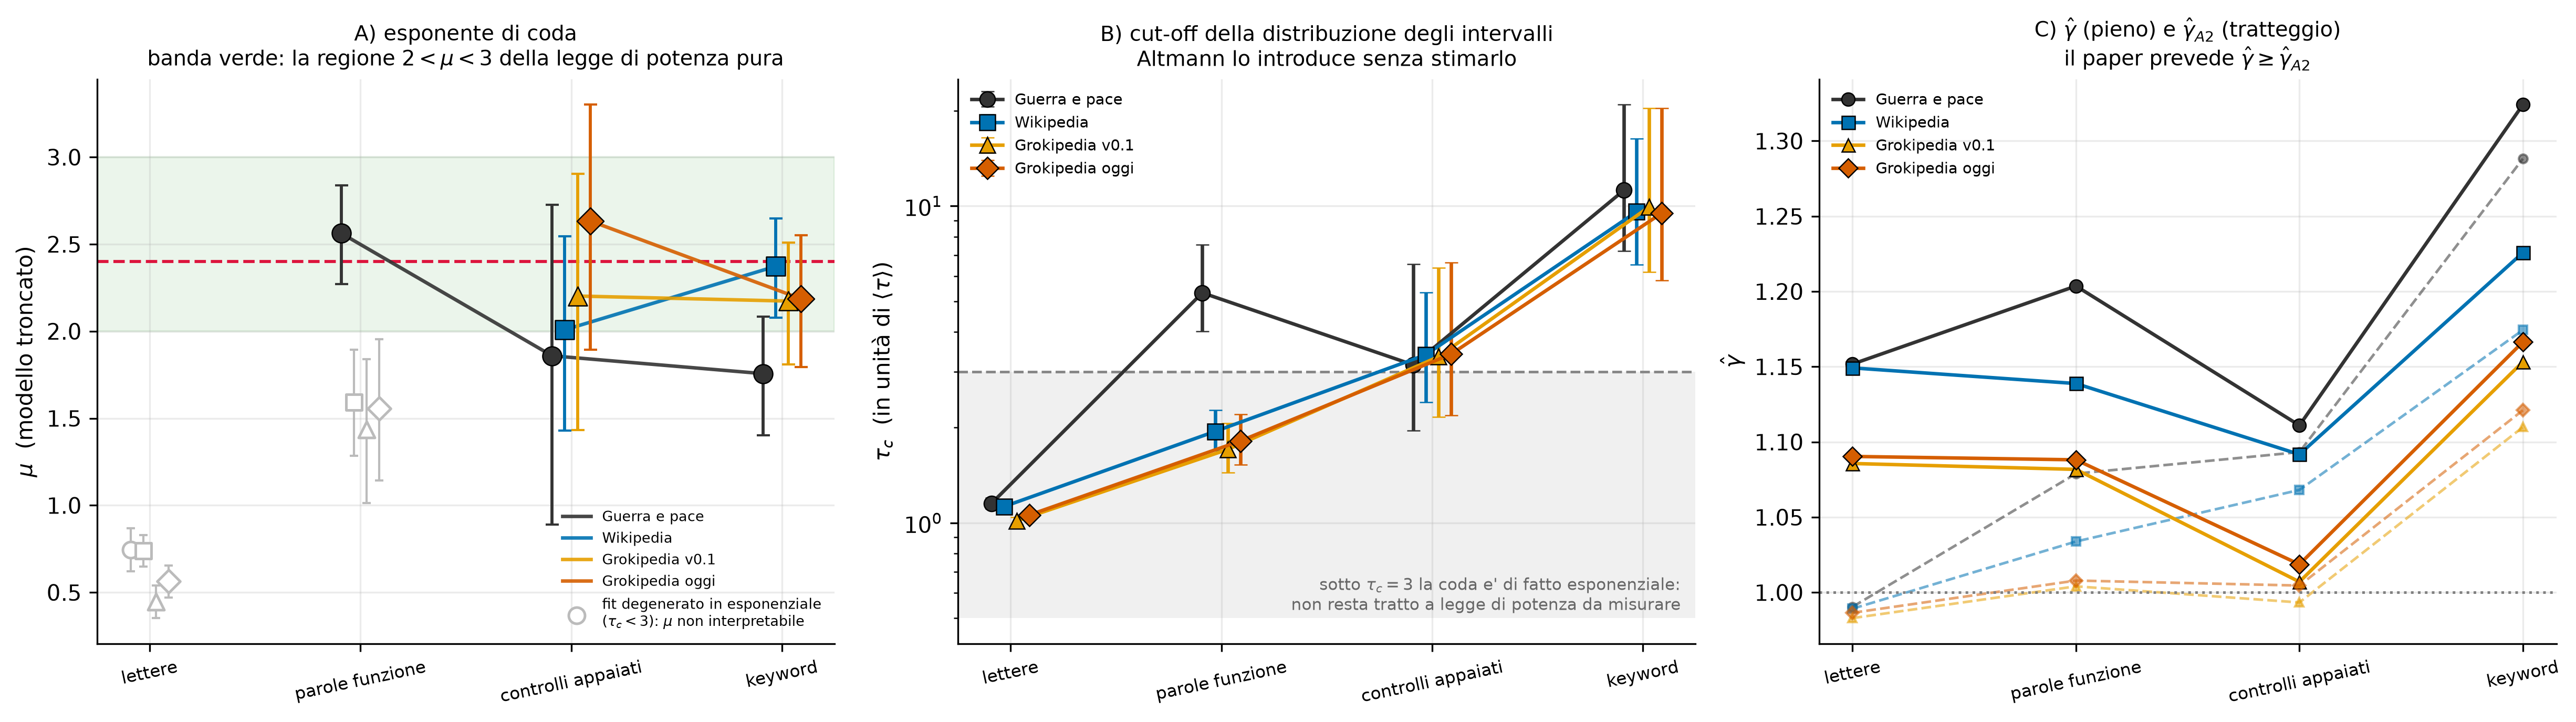
\includegraphics[width=\textwidth]{figure/cap5_esponente_coda.png}
  \caption{Stima diretta della coda della distribuzione degli intervalli. A:
  esponente $\mu$ della~\eqref{eq:coda-troncata} ai quattro livelli, con
  intervalli di confidenza di profilo; la banda verde è la regione $2<\mu<3$ in
  cui è derivata la~\eqref{eq:eq8} per la legge di potenza pura, mentre sotto il
  modello troncato adottato qui i momenti restano finiti per qualunque $\mu$ e
  la banda va letta come riferimento alla letteratura; i simboli grigi sono le
  celle in cui il fit degenera in un esponenziale e $\mu$ non è interpretabile,
  che le linee di collegamento saltano. B: cut-off
  $\tau_c$ agli stessi livelli, in unità dell'intervallo medio e con intervalli
  di confidenza di profilo; sotto la soglia tratteggiata non resta tratto a legge
  di potenza da misurare. C: $\hat\gamma$ (pieno) contro $\hat\gamma_{A2}$
  (tratteggiato) ai quattro livelli. La~\eqref{eq:disug1} è rispettata in tutte
  le celle: la curva piena sta sempre sopra la tratteggiata.}
  \label{fig:coda}
\end{figure}

\paragraph{Perché $\mu$ non serve a confrontare i corpora.}
I quattro valori non vanno però usati per ordinare i corpora, e la
Figura~\ref{fig:verosimiglianza} mostra perché: $\mu$ e $\tau_c$ sono
fortemente correlati, cosicché le regioni di confidenza congiunte sono creste
allungate anziché ellissi compatte e quelle dei tre corpora enciclopedici si
sovrappongono quasi interamente. A ciò si aggiunge la dipendenza dal punto in
cui si decide che la coda cominci: spostando $x_{\min}$ dal settantacinquesimo
al novantacinquesimo percentile $\mu$ passa da $1.65$ a $2.63$ su Wikipedia, una
variazione maggiore di ogni differenza fra corpora, e le curve si incrociano.

Di questa analisi non resta perciò un ordinamento fra corpora. Restano due
risultati, entrambi insensibili alla posizione esatta lungo la cresta: la legge
di potenza pura è rifiutata ovunque, e il cut-off cresce in modo ordinato
salendo nella gerarchia linguistica. Il cut-off è previsto
da~\cite{altmann2012} come conseguenza della discesa lungo quella stessa
gerarchia, e la sua esistenza è qui verificata invece che assunta.

\begin{figure}[htbp]
  \centering
  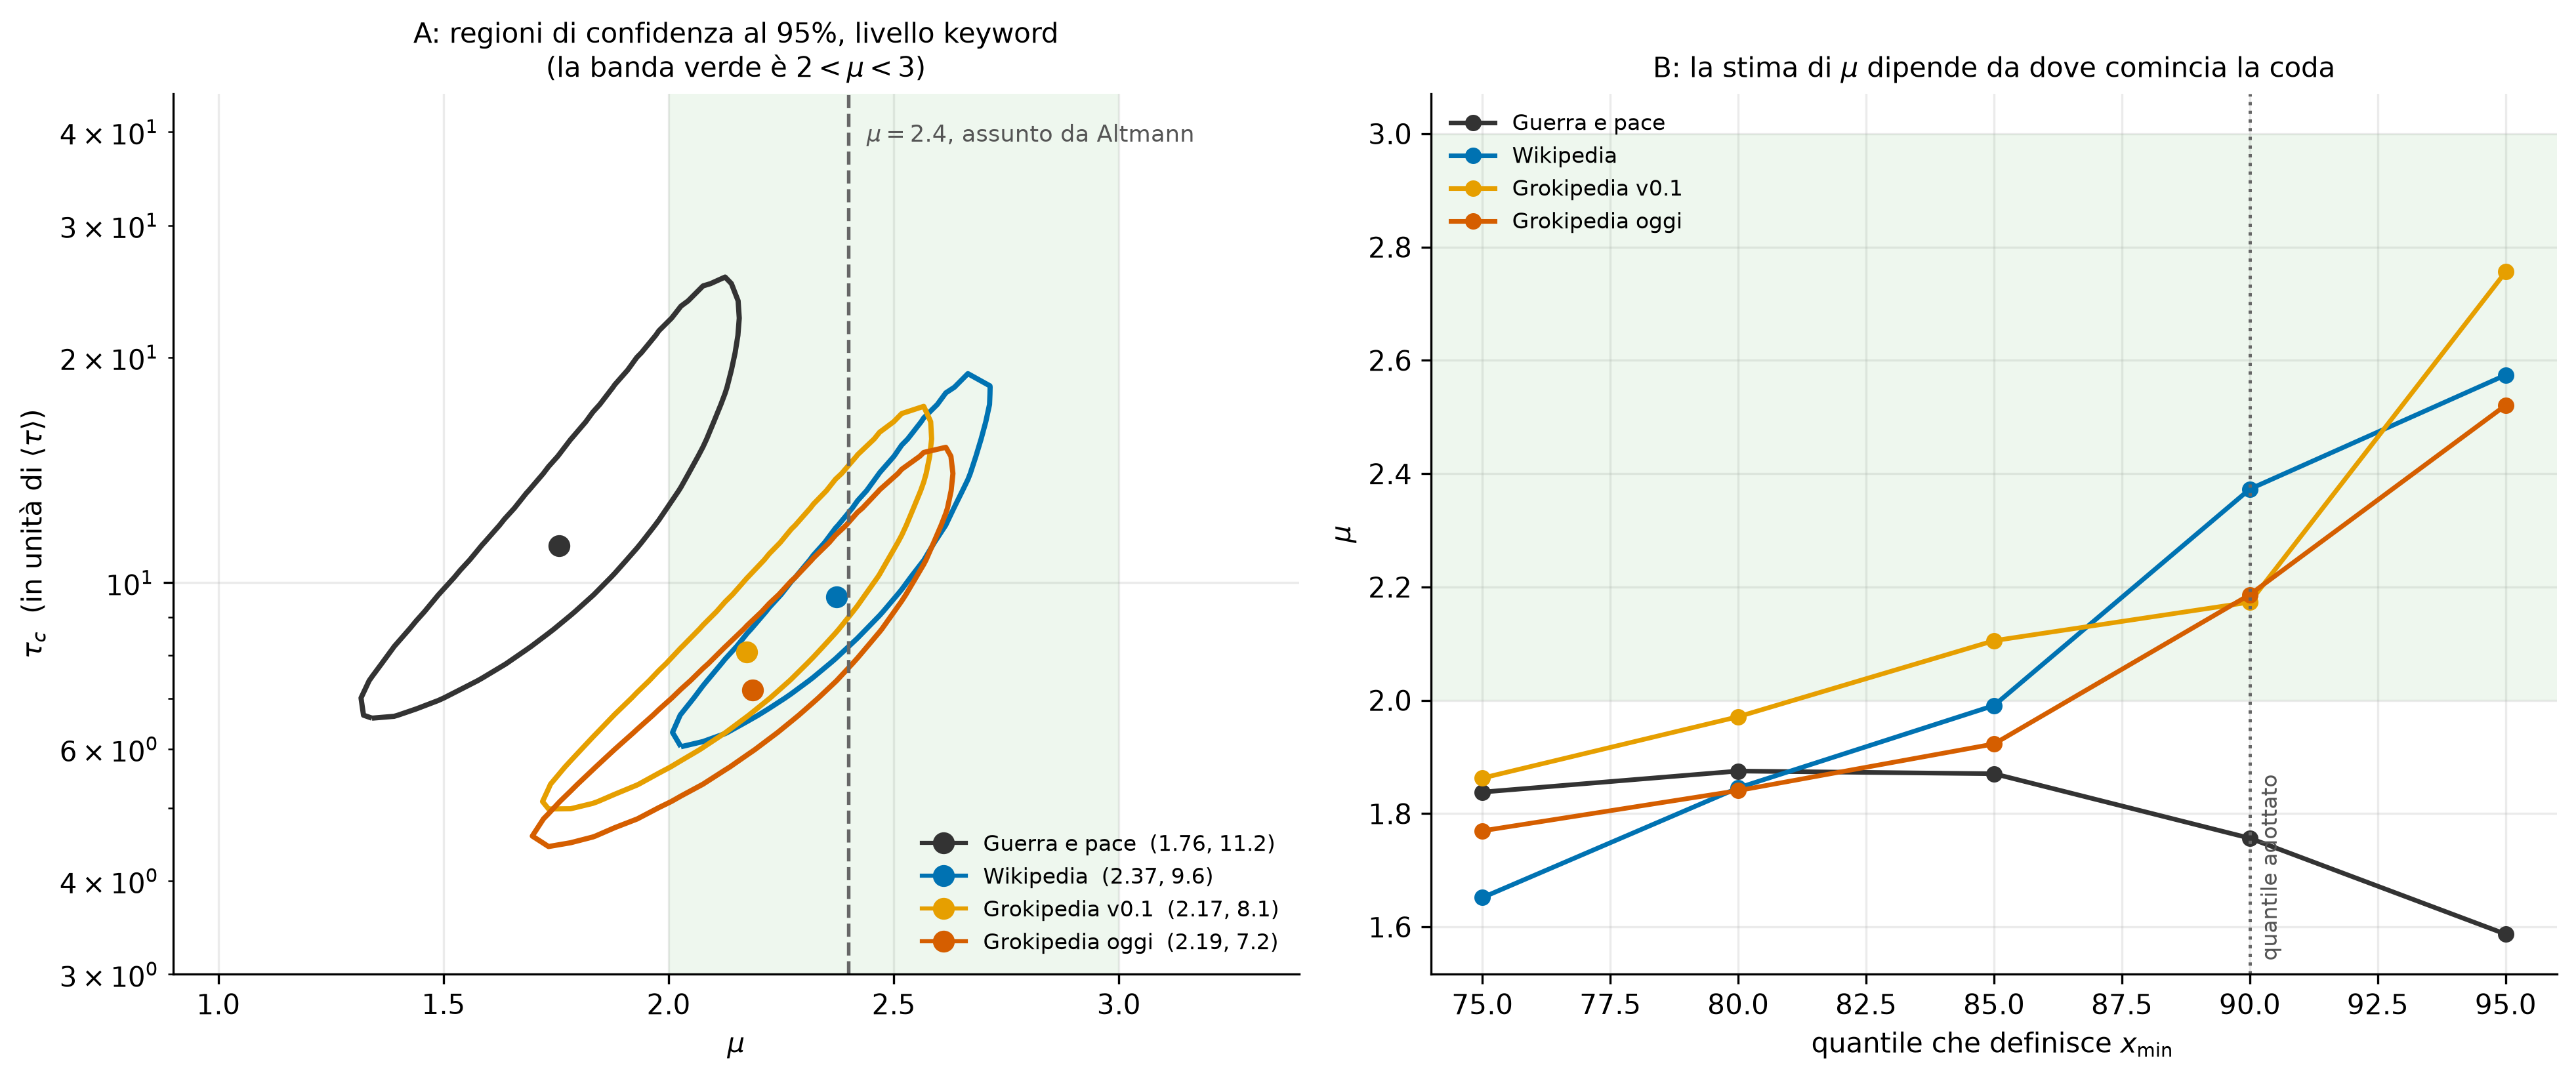
\includegraphics[width=\textwidth]{figure/cap5_verosimiglianza_coda.png}
  \caption{Perché l'esponente di coda non discrimina fra i corpora. A: regioni
  di confidenza congiunte al $95\%$ nel piano $(\mu, \tau_c)$ sul livello delle
  parole chiave, con $x_{\min}$ al novantesimo percentile; l'allungamento delle
  regioni è la correlazione fra i due parametri, e la linea tratteggiata è il
  valore $\mu = 2.4$ assunto in~\cite{altmann2012}. B: stima di $\mu$ al variare
  del quantile che definisce $x_{\min}$; le quattro curve si incrociano, cosicché
  l'ordinamento fra corpora dipende da quella scelta.}
  \label{fig:verosimiglianza}
\end{figure}

\paragraph{Il cut-off e la finestra di osservazione.} Il secondo pannello
della Figura~\ref{fig:coda} riporta $\tau_c$ ai quattro livelli, con
intervalli di confidenza di profilo. È l'altra metà di ciò
che~\cite{altmann2012} introduce senza stimare: il cut-off vi compare come
conseguenza necessaria della discesa nella gerarchia, ma non gli viene mai
assegnato un valore. Cresce in modo ordinato salendo nella gerarchia: circa
$1.1$ volte l'intervallo medio sulle lettere, dove la coda è di fatto già
esponenziale, $3.2$--$3.4$ sui controlli appaiati e $9.5$--$11.2$ sulle parole
chiave. La separazione fra i due livelli superiori è netta. Fra i quattro
corpora, invece, gli intervalli di confidenza si sovrappongono ampiamente:
neppure il cut-off ordina i corpora, e la sola cella in cui la separazione è
significativa è quella delle parole funzione del romanzo, discussa sopra.

Anche $\tau_c$ va poi letto come descrittore relativo alla lunghezza di analisi.
Ripetendo la stima sul romanzo a lunghezze crescenti, da \num{30000} a
\num{480000} caratteri, $\tau_c$ passa da $13.5$ a $94.7$: un fattore sette a
fronte di un fattore sedici sulla finestra, con un andamento non monotono che
scende prima di risalire. Il taglio non è dunque un puro artefatto, perché non
scala proporzionalmente alla finestra, ma non è nemmeno una lunghezza intrinseca
del testo. Sulla stessa serie $\mu$ si stabilizza attorno a $2.0$ alle finestre
maggiori, contro l'$1.76$ misurato alla lunghezza di lavoro: entrambi i
parametri descrivono la coda \emph{a quella lunghezza}, coerentemente con la
regola del §\ref{sec:lunghezza}.

\paragraph{Lo stimatore di Hill.} Dà sistematicamente valori più alti, $2.49$ sul
romanzo contro $1.76$ e circa $3.0$ sugli altri tre corpora contro
$2.2$--$2.4$, perché assume una legge di potenza pura su tutta la coda.
L'assenza di un plateau nel suo grafico diagnostico è ciò che ha motivato
l'adozione del modello troncato, e i suoi valori sono riportati solo a quel
titolo.

% ---------------------------------------------------------------------
\section{Entropia degli intervalli}
\label{sec:entropia-intervalli}

L'effetto di scala dichiarato nel §\ref{sec:appaiato} richiede una misura che
non risenta della lunghezza media delle frasi. È la ragione per cui il
§\ref{sec:entropia-intervalli-def} ha introdotto l'entropia degli intervalli
$J$ della~\eqref{eq:entropia-intervalli}: il logaritmo la rende invariante per
dilatazione dell'asse, cosicché frasi mediamente più lunghe non la spostano, e
la sottrazione del termine poissoniano ne cancella il bias. La grandezza è
risultata calcolabile su \num{5343} sequenze su \num{5617}, il $95\%$ del
totale.

\paragraph{Perché la misura è legittima.}
Trattandosi di una grandezza introdotta qui, la sua adozione va giustificata su
quello che fa e non su un precedente. I due ingredienti sono però entrambi
standard: l'entropia differenziale stimata per spaziature d'ordine è lo
stimatore di~\cite{vasicek1976}, e il confronto di una statistica osservata con
il valore che essa assume su un processo di Poisson di pari intensità è la
costruzione con cui in letteratura si misura la regolarità di una sequenza di
eventi, la stessa su cui poggiano la~\eqref{eq:cv} e il coefficiente
di~\cite{goh2008} usati nel resto del capitolo. Ciò che $J$ aggiunge è
l'invarianza per dilatazione, che nessuna delle due possiede e che serve qui per
una ragione specifica. Il §\ref{sec:entropia-intervalli-def} argomenta perché
debba funzionare; la validazione empirica è alla fine di questa sezione, dove la
stessa parola misurata a lunghezze diverse sposta il coefficiente di variazione
di un fattore tre e $J$ di due decimi di bit.

\paragraph{Che cosa riportano i tre pannelli.}
Il primo pannello della Figura~\ref{fig:entropia} mostra il rapporto fra $J$ e
il coefficiente di variazione sulle parole chiave. Le due misure sono
correlate, come atteso, ma la relazione non è biunivoca: a parità di
coefficiente di variazione i punti dei diversi corpora occupano fasce di $J$
diverse, il che è precisamente ciò che rende utile la seconda misura.

Il secondo pannello riporta $J$ ai quattro livelli. Sulle lettere i quattro
corpora coincidono attorno a $-0.20$, e sulle parole funzione i tre corpora
enciclopedici scendono insieme attorno a $-0.29$, con il romanzo che resta a
$-0.19$: valori negativi indicano intervalli più regolari di un
processo di Poisson. Sui due livelli superiori i corpora si separano, e sulle
parole chiave i corpora umani stanno sopra il valore poissoniano e quelli
generati vi si appoggiano: $J$ vale $+0.061$ sul romanzo e $+0.092$ su
Wikipedia, contro $-0.001$ su Grokipedia v0.1 e $-0.011$ sulla versione
attuale, questi ultimi due indistinguibili da zero. Le due enciclopedie generate
si collocano dunque sul valore poissoniano, mentre quella umana ne sta sopra:
gli intervalli fra parole chiave di Grokipedia non sono più regolari del caso,
semplicemente non sono più \emph{bursty} di esso. Il terzo pannello riporta la
distribuzione per documento e mostra che la separazione, pur con code
sovrapposte, riguarda l'intero corpus e non alcune voci.

\paragraph{La coda inferiore è fatta di soggetti di voce.}
La coda inferiore di quel pannello merita però un controllo, perché il cambio
di segno è ciò su cui l'affermazione precedente poggia. Le sequenze con $J$
più basso sono parole chiave a pieno titolo, nomi propri e non lessico di
servizio sfuggito alla lista chiusa, ma sono quasi tutte la stessa cosa: il
soggetto della voce. Fra le venti sequenze di $J$ minore, in Grokipedia
quattordici sono il soggetto dell'articolo, e in Wikipedia diciotto:
\emph{churchill}, \emph{newton}, \emph{paris}, \emph{freud}, \emph{mandela}. È
il fenomeno del §\ref{sec:tre-corpora}, che $J$ registra come gli altri
indicatori, e non è un difetto della classificazione.

Ha però una conseguenza sul cambio di segno. Escludendo i soggetti delle voci,
$54$ sequenze su $273$ in Grokipedia e $57$ in Wikipedia, tutti e tre i
corpora enciclopedici passano sopra il valore poissoniano: $+0.175$ su
Wikipedia e $+0.070$ su Grokipedia. Il divario appaiato sopravvive, $-0.087$
bit con $p < 10^{-3}$, e con esso la conclusione del paragrafo; non sopravvive
invece la lettura per segno, perché il segno negativo di Grokipedia è prodotto
dai soggetti delle voci, che il §\ref{sec:tre-corpora} ha già mostrato essere
marcatori sintattici e non semantici. Ciò che distingue i due corpora è quanto
$J$ vale, non da che parte dello zero cade.

\paragraph{Il divario appaiato.}
I confronti appaiati confermano il divario: sulle parole chiave la differenza
mediana fra Grokipedia attuale e Wikipedia vale $-0.105$ bit e quella fra la
v0.1 e Wikipedia $-0.077$ bit, entrambe con significatività inferiore a
$10^{-3}$. Sulle lettere e sulle parole funzione, per contro, le differenze sono
positive e non significative. Poiché $J$ non risente della diversa lunghezza
delle frasi, questo risultato conferma il divario del §\ref{sec:appaiato}
senza risentire di quell'effetto, ed è il punto in cui la conclusione principale
del capitolo diventa difendibile.

\paragraph{Perché il divario è più ampio sui controlli.}
Il divario è però più ampio sui controlli appaiati, $-0.209$ bit, che sulle
parole chiave, e la ragione sta in che cosa siano quei controlli. Il controllo
di una parola chiave è la parola di frequenza più vicina fra quelle che restano
dopo aver tolto le parole chiave stesse, i nomi propri e le sei parole funzione
selezionate; poiché le parole chiave sono per costruzione le più frequenti del
loro tipo, ciò che resta a quelle frequenze è in larga parte lessico di
servizio. I controlli più ricorrenti sono infatti \emph{by}, \emph{from},
\emph{with} e \emph{as} in Wikipedia, e \emph{like}, \emph{but}, \emph{that} e
\emph{this} in Grokipedia. È il livello in cui il testo generato si distingue di
più: le sue parole di servizio sono distribuite quasi uniformemente,
$J = -0.165$, mentre quelle di Wikipedia conservano un residuo di
addensamento, $J = +0.053$.

\paragraph{Composizione e stile, in parti quasi uguali.}
Le due liste di controlli sono però diverse fra loro, e la differenza potrebbe
misurare quali parole vengono selezionate anziché come sono distribuite. Le due
cause si separano restringendo il confronto alle parole che compaiono fra i
controlli di entrambi i corpora. Sono ventisei, e dodici raggiungono almeno tre
voci per corpus. Su queste il divario resta: la differenza mediana di $J$ vale
$-0.091$ bit con $p = 0.043$, e le quattro parole più spostate sono
\emph{with} ($-0.060$ contro $-0.414$), \emph{as} ($+0.227$ contro $-0.106$),
\emph{this} ($-0.005$ contro $-0.301$) e \emph{from} ($+0.057$ contro $-0.225$).
Il divario fra le medie dei due corpora, $-0.218$ bit, si scompone dunque in
$-0.128$ attribuibili alla distribuzione delle stesse parole e $-0.091$ alla
diversa composizione delle due liste, cioè in parti quasi uguali. Il valore
differisce di un centesimo dal $-0.209$ citato sopra perché quello è la mediana
delle differenze voce per voce e questo la differenza fra le medie.

La parte attribuibile alla composizione ha un contenuto proprio. I controlli di
Wikipedia sono preposizioni e ausiliari legati alla struttura del periodo, come
\emph{by}, \emph{was}, \emph{with} e \emph{for}; quelli di Grokipedia sono in
prevalenza connettivi di discorso, come \emph{like}, \emph{but}, \emph{that} e
\emph{over}. La parte attribuibile alla distribuzione descrive invece un
meccanismo: in Wikipedia una preposizione come \emph{from} si addensa dove il
contenuto la richiede, in una sezione biografica più che in una tecnica, e i suoi
intervalli ereditano il ritmo delle sezioni; in Grokipedia la stessa parola
ricorre a cadenza quasi costante lungo tutto l'articolo. Il segno negativo di $J$
dice che quella cadenza è più regolare di quella di un processo casuale, non
soltanto meno addensata.

Una verifica interna conferma la lettura. Nei controlli di Wikipedia il $93\%$
delle parole appartiene alla lista chiusa e dà $J = +0.043$, mentre il restante
$7\%$ dà $+0.188$: la classe grammaticale della parola cambia il risultato. In
Grokipedia le due quote valgono $-0.151$ e $-0.182$, indistinguibili fra loro.
Nel testo generato la regolarità degli intervalli non dipende da che tipo di
parola si stia guardando, ed è la stessa compressione uniforme della variabilità
lessicale che il §\ref{sec:sintesi-cap5} indica come conclusione del capitolo,
osservata al livello in cui si manifesta con più forza.

\paragraph{Stabilità rispetto alla lunghezza di analisi.}
Una validazione indipendente riguarda la dipendenza dalla lunghezza. Passando
da \num{40000} caratteri al romanzo intero, il coefficiente di variazione della
parola \emph{prince} cambia di un fattore $3.08$, mentre il suo $J$ si sposta di
$0.21$ bit; per la parola \emph{pierre} il coefficiente cambia di un fattore
$3.49$ e $J$ di $0.08$ bit. I due numeri non sono direttamente confrontabili,
perché il coefficiente di variazione è un rapporto e $J$ un logaritmo: uno
spostamento di $0.21$ bit corrisponde a un fattore $2^{0.21} = 1.16$ sulla
dispersione efficace degli intervalli, e uno di $0.08$ bit a un fattore $1.06$.
Riportate alla stessa scala, le due derive stanno nel rapporto di $2.7$ e $3.3$
in favore di $J$. La nuova misura è dunque circa tre volte più stabile rispetto
alla lunghezza di analisi di quella che sostituisce, il che ne conferma
l'utilità al di là del problema specifico per cui era stata introdotta.

\begin{figure}[htbp]
  \centering
  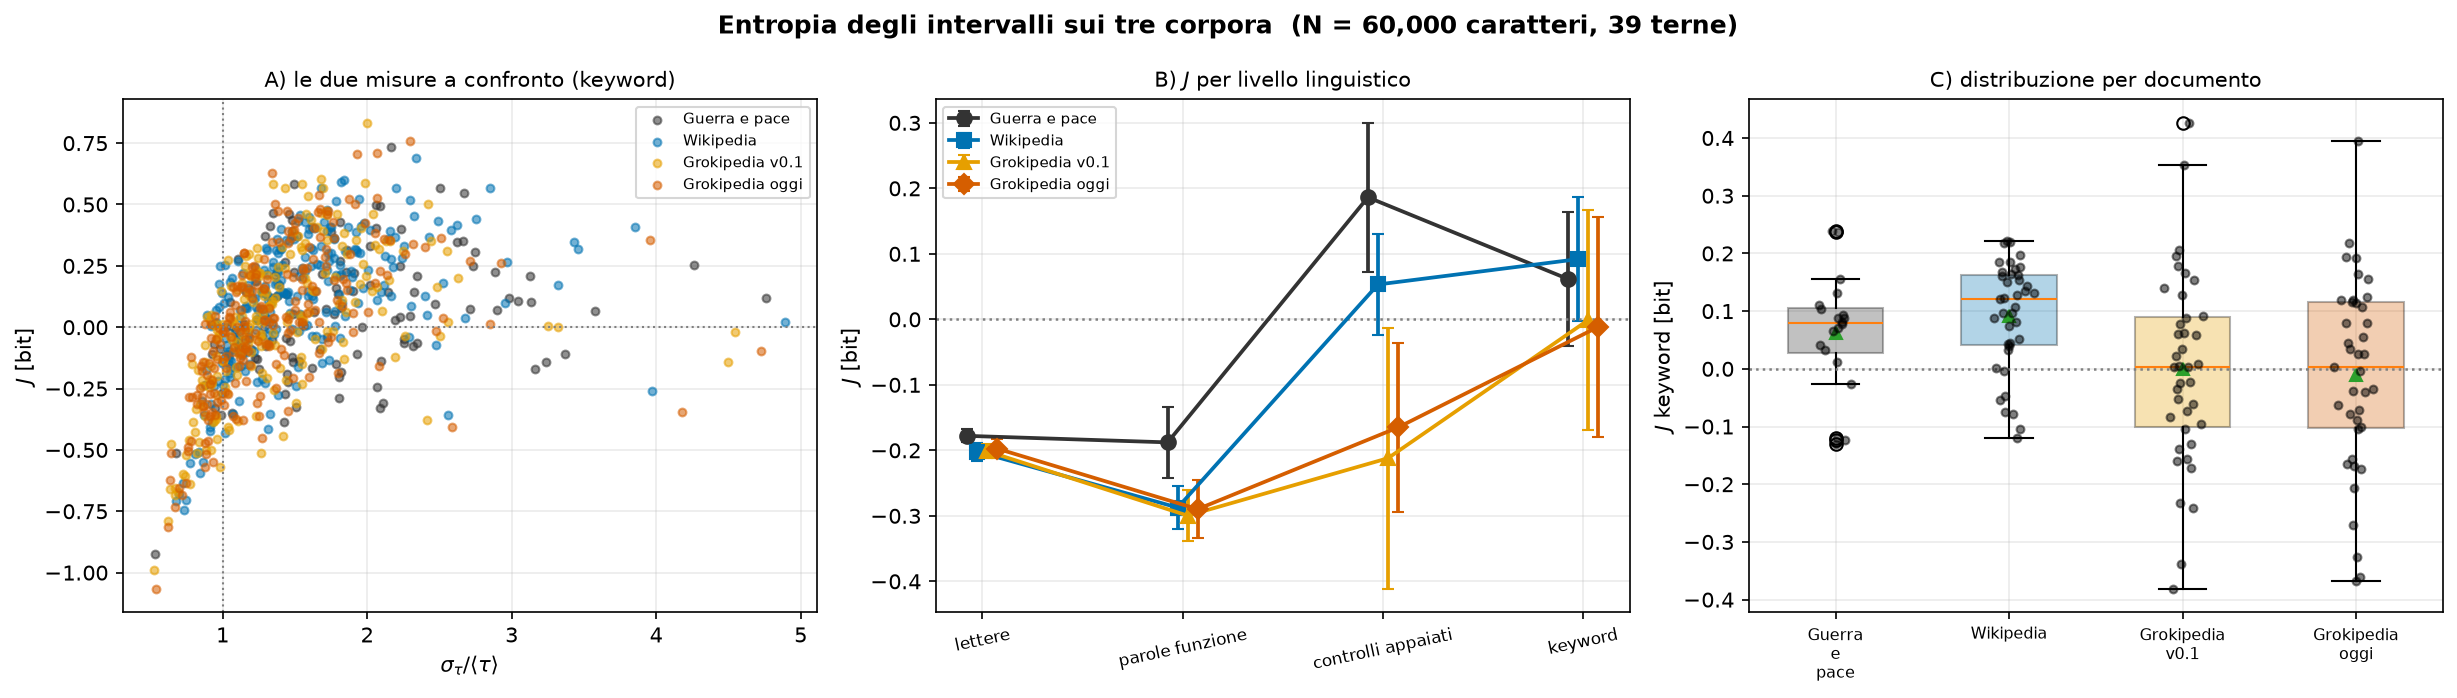
\includegraphics[width=\textwidth]{figure/cap5_entropia_intervalli.png}
  \caption{Entropia degli intervalli. A: relazione fra $J$ e coefficiente di
  variazione sulle parole chiave, un punto per sequenza. B: $J$ ai quattro
  livelli linguistici, con deviazioni standard fra testi; valori negativi
  indicano intervalli più regolari di un processo di Poisson. C: distribuzione
  di $J$ sulle parole chiave documento per documento. La misura è invariante per
  dilatazione dell'asse dei caratteri e non risente quindi della diversa
  lunghezza delle frasi nei due corpora enciclopedici.}
  \label{fig:entropia}
\end{figure}

% ---------------------------------------------------------------------
\section{Quanto pesa la definizione dei livelli lessicali}
\label{sec:effetto-stoplist}

Il paragrafo \emph{Come vengono separati i livelli lessicali} del
§\ref{sec:scelte} ha documentato l'estensione della lista chiusa di parole funzione da
\num{133} a \num{215} voci e la ragione per cui era necessaria. Questa sezione
riporta di quanto si spostano i risultati, perché lo spostamento non è
trascurabile e la scelta deve restare verificabile.

Il pannello A della Figura~\ref{fig:effetto-stoplist} riporta quali parole la
lista originaria lasciava passare fra le parole chiave di Grokipedia, e in
quante voci ciascuna: nell'elenco corrispondente di Wikipedia non ne compare
nessuna, e le sue sette parole sono distinte fra loro, ciascuna in una sola
voce.

\begin{table}[htbp]
  \centering
  \begin{tabular}{lcccc}
    \toprule
    & \multicolumn{2}{c}{lista originaria} & \multicolumn{2}{c}{lista estesa} \\
    \cmidrule(lr){2-3}\cmidrule(lr){4-5}
    & Wikipedia & Grok. oggi & Wikipedia & Grok. oggi \\
    \midrule
    keyword più bursty del controllo & $0.685$ & $0.630$ & $0.692$ & $0.740$ \\
    idem, su $\hat\gamma$ & $0.736$ & $0.663$ & $0.747$ & $0.791$ \\
    $\sigma_\tau/\langle\tau\rangle$ keyword & $1.530$ & $1.289$ & $1.536$ & $1.379$ \\
    divario appaiato, keyword & \multicolumn{2}{c}{$-0.230$} & \multicolumn{2}{c}{$-0.167$} \\
    divario appaiato, controlli & \multicolumn{2}{c}{$-0.122$} & \multicolumn{2}{c}{$-0.157$} \\
    $J$ keyword & $+0.086$ & $-0.069$ & $+0.092$ & $-0.011$ \\
    $\mu$ keyword & $2.38$ & $2.52$ & $2.37$ & $2.19$ \\
    quadrante basso-sinistra & $5.1\%$ & $24.5\%$ & $5.1\%$ & $14.3\%$ \\
    \bottomrule
  \end{tabular}
  \caption{Effetto della definizione dei livelli lessicali sui risultati del
  capitolo. Le righe dei divari appaiati riportano un solo valore perché
  misurano la differenza fra i due corpora. Le lettere e le parole funzione non
  compaiono perché nessuna parola cambia livello a quelle altezze: i loro valori
  coincidono a tutte le cifre riportate nel capitolo.}
  \label{tab:effetto-stoplist}
\end{table}

La Tabella~\ref{tab:effetto-stoplist} riporta il confronto. Tre risultati
cambiano in modo sostanziale. Il primo è il test interno: con la lista
originaria Grokipedia sembrava battere il proprio controllo appaiato meno spesso
di Wikipedia, e l'ordinamento fra i corpora appariva netto; con la lista estesa
l'ordine si inverte, e la differenza fra le due enciclopedie sparisce. Il
pannello B della figura mostra i due esiti sovrapposti. Il secondo è l'entropia
degli intervalli, il cui valore sulle parole chiave passa da $-0.069$ a
$-0.011$, cioè da un cambio di segno netto a uno indistinguibile da zero. Il
terzo è l'esponente di coda, che su Grokipedia scende da $2.52$ a $2.19$,
avvicinandosi a quello di Wikipedia anziché allontanarsene.

Restano invece stabili il divario appaiato complessivo, che si riduce da
$-0.230$ a $-0.167$ senza perdere significatività, il coefficiente di variazione
delle parole chiave, e l'intera decomposizione della~\eqref{eq:eq4}. Non si
muovono di una cifra, come è ovvio, i livelli delle lettere e delle parole
funzione.

La lezione metodologica vale al di là di questo caso. La distinzione fra
parole di contenuto e parole di servizio è la premessa dell'intero protocollo
di~\cite{altmann2012}, e viene qui operata da una lista chiusa che il paper
non specifica. Quando i corpora confrontati hanno abitudini lessicali diverse,
e un modello linguistico ne ha rispetto a un redattore umano, una lista
incompleta non introduce un rumore simmetrico: sposta sistematicamente in un
solo corpus il confine fra i due livelli, e produce un divario che non c'è.

\begin{figure}[htbp]
  \centering
  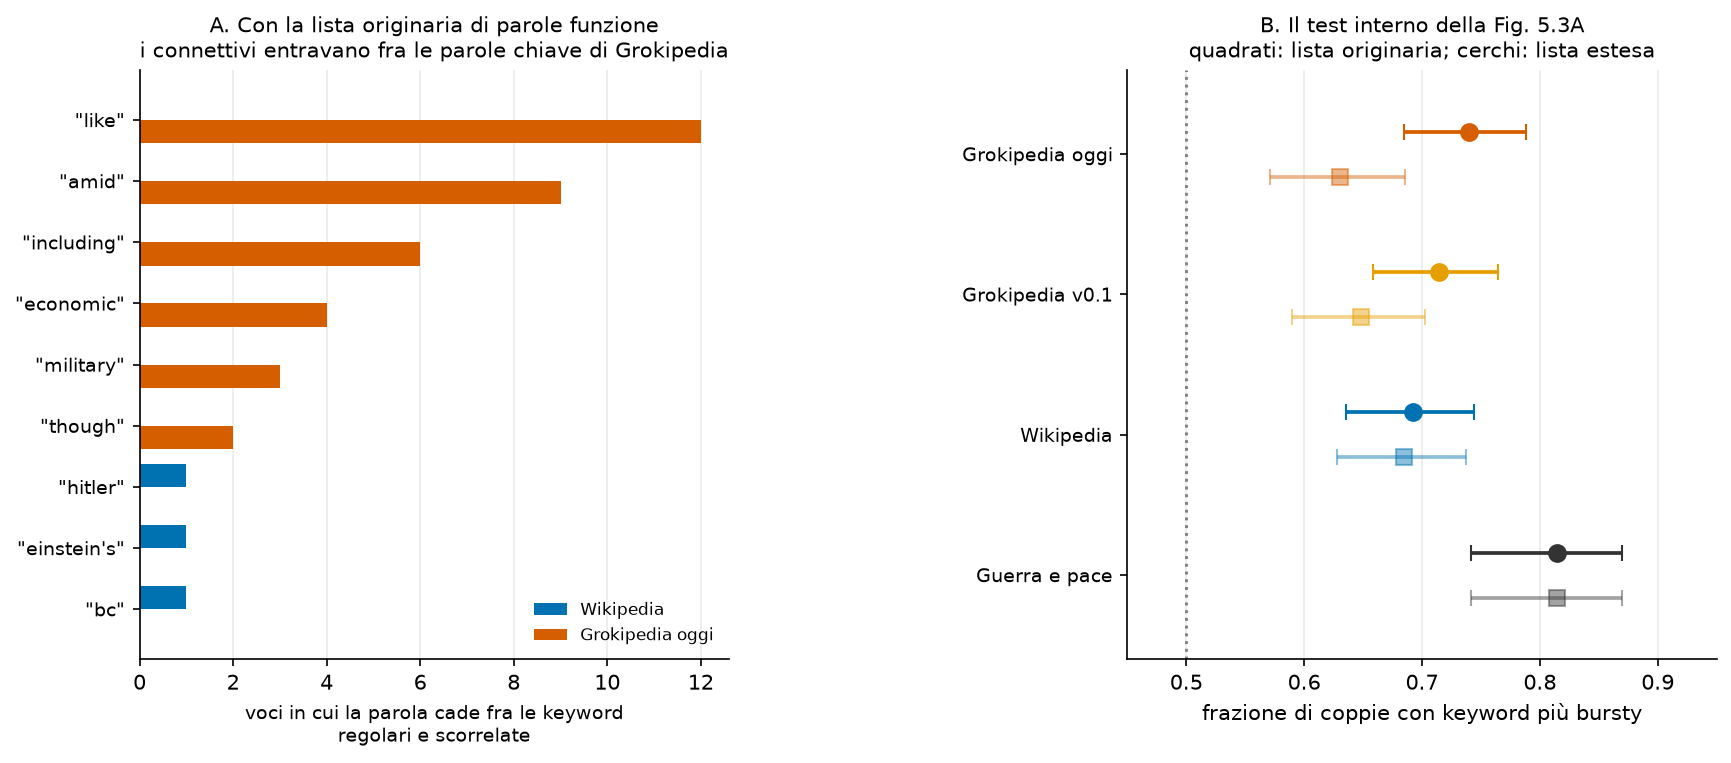
\includegraphics[width=\textwidth]{figure/cap5_effetto_stoplist.png}
  \caption{Effetto della definizione dei livelli lessicali. A: con la lista di
  funtori originaria, quali parole cadevano fra le parole chiave classificate
  come regolari e scorrelate, contate come numero di voci in cui ciò accadeva;
  le prime tre di Grokipedia sono connettivi, e in Wikipedia non compaiono. B:
  il test interno della Figura~\ref{fig:tre-corpora}A con le due
  classificazioni, quadrati per la lista originaria e cerchi per quella estesa,
  con intervalli di confidenza al $95\%$.}
  \label{fig:effetto-stoplist}
\end{figure}

% ---------------------------------------------------------------------
\section{Che cosa il testo generato non riproduce}
\label{sec:sintesi-cap5}

Il testo generato possiede correlazioni a lungo raggio, e ai livelli bassi della
gerarchia linguistica le possiede quasi nella stessa misura del testo umano:
sulle lettere i quattro corpora sono indistinguibili per coefficiente di
variazione, per entropia degli intervalli e per quota di burstiness, e sulle
parole funzione la differenza è piccola, benché significativa. Al livello delle parole il divario si apre, e vale più di un ordine
di grandezza rispetto a quello misurato sui caratteri.

Il divario non distingue però le parole che portano il contenuto dai controlli a
frequenza appaiata. I due valori sono quasi uguali alla lunghezza di lavoro,
$-0.157$ e $-0.167$, e si invertono a quella di controllo
(§\ref{sec:robustezza-neff}); e il test che chiede se la parola chiave superi il
proprio controllo \emph{dentro lo stesso testo} dà a Grokipedia un esito pari a
quello di Wikipedia, anzi lievemente migliore. Il meccanismo descritto
in~\cite{altmann2012} è dunque presente nel testo generato, e con la stessa
efficacia: ciò che manca è l'ampiezza con cui le parole, di contenuto e non, si
addensano.

Non si tratta dunque di una persistenza tematica assente, perché la distinzione
fra parole tematiche e parole ordinarie il modello la produce; si tratta di una
compressione uniforme della variabilità lessicale, che riduce la burstiness di
tutte le parole senza alterare il rapporto fra le une e le altre. Vale ancora la
distinzione posta nel §\ref{sec:intro-linguaggio} fra riprodurre le proprietà
statistiche del linguaggio e riprodurre il meccanismo che le genera, ma
applicata a un livello più basso di quanto la prima lettura suggerisse.

Ciò che il capitolo misura è la distanza fra due enciclopedie appaiate titolo
per titolo, e null'altro. Il deficit è osservato su Grokipedia, cioè su un unico
sistema generativo, in un unico dominio e in una sola lingua: nulla di quanto
riportato qui stabilisce che sia una proprietà dei modelli linguistici in
generale anziché di quel sistema. Il Capitolo~\ref{cap:risultati1} non offre un
appoggio indipendente su questo punto: misura un altro corpus, con grandezze
che non arrivano al livello a cui il divario si manifesta.

%
%  Tre lunghezze di analisi con corpora diversi, da non confondere:
%    fattibilità  50 000 caratteri, 40 voci  (§5.2)
%    analisi      60 000 caratteri, 39 terne (§5.3--5.7)
%    robustezza   80 000 caratteri, 35 terne (§5.8)
% =====================================================================

\chapter{Burstiness lessicale in corpora umani e generativi}
\label{cap:risultati2}

% ---------------------------------------------------------------------
\section{Perché un secondo corpus}
\label{sec:perche-wiki}

Questo capitolo nasce da un esito negativo del precedente. Il
§\ref{sec:fallimenti} ha mostrato che dei \num{242} documenti generati lungo lo
sweep soltanto due non ricadono in alcuna modalità di degenerazione, ed entrambi
si trovano a $T = 1.0$. Il protocollo introdotto nel §\ref{sec:burst} è però un
protocollo semantico: richiede di individuare in ciascun testo le parole che ne
portano il contenuto e di misurare come si distribuiscono le distanze fra le
loro occorrenze successive. Su un testo che ripete lo stesso ciclo di parole, o
su una sequenza degenerata nel senso opposto, 
quelle distanze si calcolano ancora ma non misurano più la
persistenza di un tema. Applicare il protocollo al corpus dello sweep
restituirebbe numeri privi di contenuto.

Il confronto viene quindi spostato su un dominio in cui la qualità del testo
non è una variabile. Wikipedia e Grokipedia trattano le stesse voci, la prima
scritta da esseri umani e la seconda generata da un modello linguistico, ed
entrambe producono prosa espositiva ben formata. Appaiare le due enciclopedie
per titolo tiene inoltre fisso l'argomento trattato: la voce
\emph{Albert Einstein} di Wikipedia e quella di Grokipedia parlano della stessa
cosa, e qualunque differenza nella statistica degli intervalli non può essere
attribuita a un argomento diverso. I corpora sono descritti nel §\ref{sec:corpora}, e le
due versioni di Grokipedia nel §\ref{sec:paternita}.

Il romanzo di riferimento resta nell'analisi come ancora letteraria: è il
dominio su cui il protocollo è stato formulato, e serve a dire quanto la prosa
enciclopedica si discosti già di per sé dal caso studiato in origine.

% ---------------------------------------------------------------------
\section{Il protocollo regge sulla prosa enciclopedica}
\label{sec:fattibilita}

Prima di confrontare due enciclopedie occorre stabilire che l'effetto da
confrontare esista nella prima. Il protocollo di Altmann è stato costruito e
validato su romanzi, e la prosa enciclopedica ha una struttura diversa: non ha
trama, procede per sezioni tematiche dichiarate da titoli, e la persistenza di
un argomento vi si manifesta in modo più rigido. Che le parole di contenuto vi
risultino più \emph{bursty} dei propri controlli non è quindi scontato.

La verifica è stata condotta su \num{40} voci di Wikipedia troncate a
\num{50000} caratteri, contro \num{20} segmenti del romanzo della stessa
lunghezza: è la fase di fattibilità della Tabella~\ref{tab:fasi}, l'unica del
capitolo a impiegare quella lunghezza e quel numero di voci, e i suoi
denominatori non vanno confusi con quelli delle sezioni successive. La
Figura~\ref{fig:wiki-fattibilita} ne riporta l'esito. Il primo
pannello confronta ciascuna parola chiave con il proprio controllo appaiato in
frequenza e riporta la quota di confronti vinti dalla parola chiave: il valore
$0.5$ corrisponde all'assenza di effetto. Su Wikipedia la quota vale
$197/280 = 0.704$ per il coefficiente di variazione e $216/280 = 0.771$ per
l'esponente di correlazione, con estremi inferiori degli intervalli di
confidenza pari a $0.65$ e $0.72$: l'effetto esiste. Sul romanzo le stesse
quote valgono $104/140 = 0.743$ e $123/140 = 0.879$, cioè sono più alte, ma la
differenza non annulla il segnale enciclopedico.

Il secondo pannello mostra da dove viene quel segnale, ed è utile precisare
come i suoi valori siano costruiti, perché la stessa procedura vale per tutte
le figure per livello del capitolo. Dentro ciascun testo si selezionano più
sequenze per livello: diciannove lettere, sei parole funzione, sette parole
chiave e i sette controlli appaiati. Per ognuna si misura
$\sigma_\tau/\langle\tau\rangle$ sui suoi intervalli. I valori delle sequenze
dello stesso livello si mediano poi dentro il testo, ottenendo un
numero per coppia (testo, livello); infine si media su tutti i testi del
corpus, ed è questo secondo valore a comparire nel pannello, con la barra
d'errore data dalla deviazione standard fra testi. Con questa costruzione il
coefficiente di variazione $CV$ cresce salendo lungo i quattro livelli in entrambi
i corpora e con lo stesso andamento: le lettere stanno sotto l'unità, cioè si
distribuiscono in modo più regolare di un processo di Poisson, mentre le
parole chiave arrivano a $1.51$ su Wikipedia e a $1.62$ sul romanzo. Il terzo
pannello riporta la distribuzione dei singoli testi attorno a quelle medie e
mostra che la sovrapposizione fra i due corpora è ampia, con mediane vicine e
code che si intersecano.

Il rapporto fra le due burstiness delle parole chiave vale $0.93$: la prosa
enciclopedica è meno \emph{bursty} del romanzo, ma dello stesso ordine. Il protocollo
regge, e il confronto con Grokipedia ha un segnale da rilevare.

\begin{figure}[htbp]
  \centering
  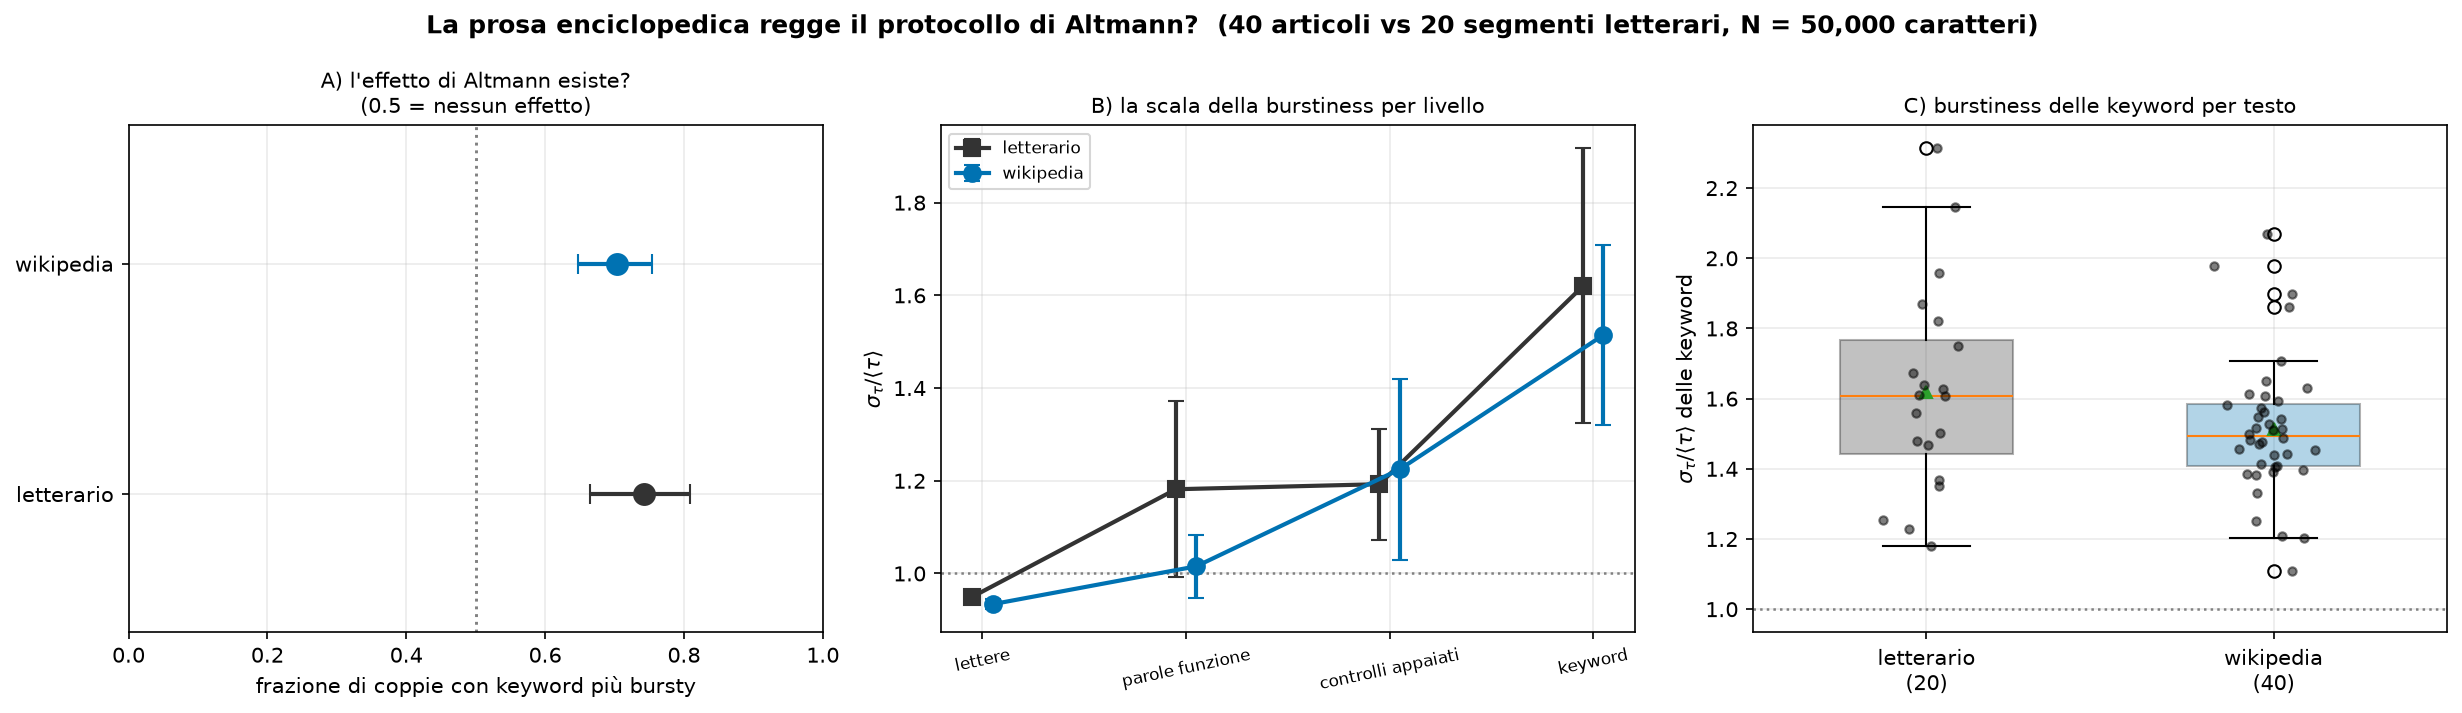
\includegraphics[width=\textwidth]{figure/cap5_wiki_altmann.png}
  \caption{Test di fattibilità del protocollo su prosa enciclopedica, condotto
  su \num{40} voci di Wikipedia e \num{20} segmenti letterari a \num{50000}
  caratteri. A: quota di confronti in cui la parola chiave supera il proprio
  controllo appaiato in frequenza, con intervallo di confidenza al $95\%$; la
  linea punteggiata a $0.5$ è l'assenza di effetto. B: coefficiente di
  variazione degli intervalli ai quattro livelli linguistici. C: distribuzione
  della burstiness delle parole chiave testo per testo. Questa è l'unica figura
  del capitolo costruita su \num{40} voci e \num{50000} caratteri; tutte le
  successive usano \num{39} terne e \num{60000} caratteri.}
  \label{fig:wiki-fattibilita}
\end{figure}

% ---------------------------------------------------------------------
\section{L'effetto nei tre corpora}
\label{sec:tre-corpora}

L'analisi principale confronta Wikipedia, le due versioni di Grokipedia e
l'ancora letteraria su \num{39} terne complete, troncate a \num{60000}
caratteri. La voce esclusa è \emph{Buddhism}, per la ragione riportata nel
§\ref{sec:paternita}: la sua versione v0.1 è ricopiata da Wikipedia, e in un
disegno appaiato un titolo che cade in un corpus deve cadere in tutti.

\paragraph{La finestra su cui l'esponente è stimato.}
L'esponente di correlazione $\hat\gamma$ è ottenuto interpolando
la~\eqref{eq:sigma} nell'intervallo fisso $t \in (100, 2000)$ caratteri.
\cite{altmann2012} adotta invece una regola relativa e ferma la finestra
all'uno per cento della lunghezza del testo. Le due scelte non sono ordinabili
una volta per tutte: applicata ai romanzi interi che quel lavoro analizza la
regola relativa dà un tetto dell'ordine di \num{10000} caratteri, molto più
largo di quello adottato qui; applicata alle finestre da \num{60000} caratteri
di questo capitolo dà $t < 600$, molto più stretto. L'intera catena è stata
ripetuta anche con la seconda. Il
livello medio di $\hat\gamma$ si abbassa di qualche centesimo, sulle parole
chiave da $1.23$ a $1.18$ per Wikipedia e da $1.32$ a $1.22$ per il romanzo,
ma l'ordinamento fra i corpora resta identico a tutti e quattro i livelli. Il
divario appaiato fra Grokipedia attuale e Wikipedia sulle parole chiave passa
da $-0.049$ a $-0.076$, cioè si accentua invece di ridursi, e resta
significativo in entrambi i casi. Le conclusioni di questo capitolo non
dipendono dunque dalla finestra scelta.

\paragraph{Tre modi di leggere il confronto.}
La Figura~\ref{fig:tre-corpora} riporta i tre modi in cui il confronto può
essere letto. Il primo pannello ripete il test del paragrafo precedente sui
quattro corpora: la quota di confronti vinti dalle parole chiave vale
$114/140 = 0.814$ sul romanzo, $189/273 = 0.692$ su Wikipedia,
$195/273 = 0.714$ su Grokipedia v0.1 e $202/273 = 0.740$ su Grokipedia nella
versione attuale. Ripetendo lo stesso test sull'esponente di correlazione
$\hat\gamma$ anziché sulla burstiness, la quota di confronti vinti dalle parole
chiave vale $0.907$ sul romanzo, $0.747$ su Wikipedia, $0.769$ su Grokipedia
v0.1 e $0.791$ su Grokipedia nella versione attuale.
L'effetto esiste ovunque, con tutti e quattro gli
intervalli di confidenza interamente sopra $0.5$, ed è massimo sul romanzo;
fra le due enciclopedie, però, non distingue: i valori di Grokipedia sono anzi
lievemente superiori a quelli di Wikipedia, con intervalli che si sovrappongono.
La domanda a cui questo pannello risponde è se la parola chiave superi il
proprio controllo a frequenza appaiata dentro lo stesso testo, e la
risposta è che ciò accade con la stessa frequenza nei due corpora enciclopedici.
Il deficit di Grokipedia, misurato dai pannelli successivi, non riguarda dunque
l'esistenza del meccanismo ma il livello assoluto della burstiness.

Il secondo pannello mostra il coefficiente di variazione ai quattro livelli e
rende visibile dove la differenza si concentra. Sulle lettere i quattro corpora
sono indistinguibili, tutti compresi fra $0.922$ e $0.950$, e sulle parole
funzione la separazione resta modesta, da $0.967$ a $1.192$. Il divario si apre
ai due livelli lessicali: sui controlli appaiati il romanzo raggiunge $1.262$,
Wikipedia $1.190$ e le due versioni di Grokipedia $1.044$ e $1.055$; sulle
parole chiave rispettivamente $1.789$, $1.536$, $1.387$ e $1.379$. 
Il terzo pannello riporta la stessa quantità testo per testo,
e mostra che la separazione non è l'effetto di pochi articoli anomali: le
distribuzioni di Wikipedia e di Grokipedia si sovrappongono, ma le loro mediane
differiscono di circa $0.25$ e la coda superiore di Wikipedia è più popolata.

\begin{figure}[htbp]
  \centering
  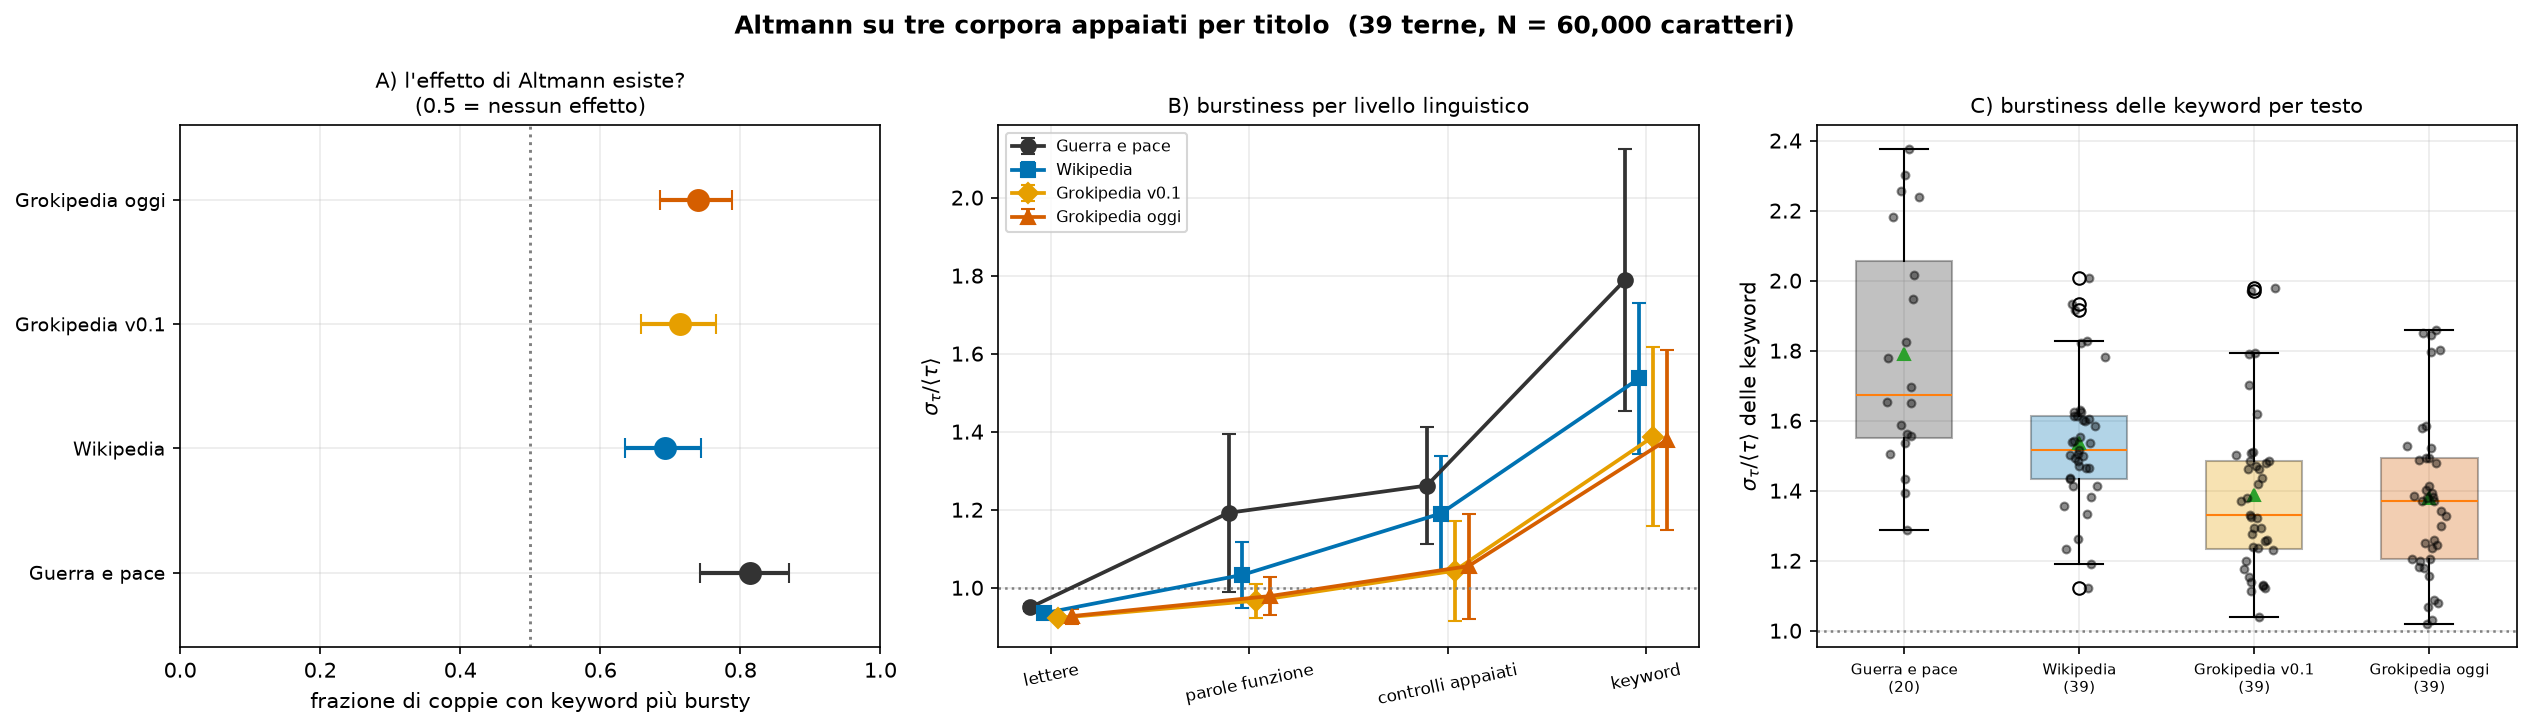
\includegraphics[width=\textwidth]{figure/cap5_tre_corpora.png}
  \caption{Il protocollo di Altmann sui quattro corpora, \num{39} terne
  appaiate per titolo a \num{60000} caratteri. A: quota di confronti vinti dalle
  parole chiave, con intervallo di confidenza al $95\%$. B: coefficiente di
  variazione degli intervalli ai quattro livelli linguistici; le barre sono
  deviazioni standard fra testi. C: burstiness delle parole chiave testo per
  testo, con mediana, quartili e singoli punti sovrapposti. Il numero di testi
  per corpus è indicato sotto ciascuna colonna.}
  \label{fig:tre-corpora}
\end{figure}

\paragraph{L'ancora letteraria è un testo, non un genere.} Il primato del
romanzo sui due livelli lessicali non sopravvive al cambio di testo. Ripetendo
l'intera misura su tre altri romanzi inglesi trattati esattamente come
\emph{Guerra e pace}, cioè \emph{Moby Dick}, \emph{Middlemarch} e \emph{David
Copperfield}, gli stessi impiegati come controllo nel
§\ref{sec:coda-risultati}, sulle parole chiave si ottiene $1.55$, $1.54$ e
$1.63$, cioè valori sostanzialmente pari a quello di Wikipedia e ben al di
sotto dell'$1.79$ di \emph{Guerra e pace}; alle parole funzione si ottiene
$1.03$, $1.08$ e $1.09$, contro l'$1.19$ del romanzo di riferimento e l'$1.03$
di Wikipedia. La distanza fra prosa letteraria e prosa enciclopedica non è
dunque un fatto generale, e l'ancora letteraria di questo capitolo va letta
per ciò che è: un termine di paragone concreto, non la misura di un genere.
Nulla di ciò che segue vi poggia, perché il risultato del capitolo è un
confronto appaiato fra le due enciclopedie, dove il romanzo non entra.

Il null model A1 restituisce un esponente medio di $0.983$ su tutte le celle,
in accordo con l'unità che deve dare per costruzione: la procedura di stima si
comporta come nel §\ref{sec:validazione} anche su questi corpora.

\paragraph{L'analogo della Figura~2 di~\cite{altmann2012}.}
La Figura~\ref{fig:altmann-fig2} riproduce sui quattro corpora la costruzione
con cui~\cite{altmann2012} presenta il proprio risultato principale, e permette
di verificarne l'aderenza riga per riga. Per ogni corpus vengono mostrate una
lettera e una parola di contenuto, ciascuna con la distribuzione cumulata degli
intervalli e con la crescita della varianza del conteggio, accanto alle stesse
curve calcolate sui due null model.

\paragraph{Quale parola mostrare.} La scelta della parola da mostrare pone un
problema che il caso della lettera non ha. Selezionare la parola chiave più
ricorrente del corpus, che è il criterio più immediato, produce oggetti
strutturalmente diversi nei due tipi di prosa: in un romanzo pesca il nome di
un personaggio, presente solo nelle scene in cui il personaggio compare,
mentre in un'enciclopedia pesca il soggetto della voce, che ricorre in quasi
ogni frase. Le due parole finirebbero alle code opposte delle rispettive
distribuzioni di burstiness, al $96$ e al $2$ percentile, e la figura
confronterebbe due casi estremi anziché due casi tipici. La parola mostrata è
quindi quella con $\sigma_\tau/\langle\tau\rangle$ più vicino alla mediana del
proprio corpus, fra quelle con almeno \num{40} occorrenze; il percentile
effettivo è riportato sopra ciascun pannello e sta fra $45$ e $57$ in tutti e
quattro i corpora. Il caso escluso ha però un interesse proprio, ed è ripreso
subito dopo la figura.

\paragraph{Che cosa mostrano le quattro righe.}
Il comportamento è allora quello descritto nel §\ref{sec:origini}, e vale su
tutte e quattro le righe. Sulla lettera la cumulata decade rapidamente e
l'esponente del null model A2 si dispone attorno all'unità, $0.94$ sul romanzo,
$0.90$ su Wikipedia, $0.94$ sulla v0.1 e $1.05$ sulla versione attuale di
Grokipedia, perché a quel livello la burstiness non contribuisce. Lo scarto
massimo da uno vale un decimo, ed è quanto ci si attende su una singola
sequenza: aggregando tutte le \num{2603} sequenze di livello letterale dei
quattro corpora $\hat\gamma_{A2}$ vale fra $0.983$ e $0.990$, con una
dispersione fra sequenze di $0.044$, cosicché i quattro valori della figura
stanno tutti entro due deviazioni standard dall'unità. Un solo caso per corpus
non permette dunque una lettura più fine di così.

Sulla parola di contenuto la cumulata ha coda larga, con
$\sigma_\tau/\langle\tau\rangle$ fra $1.23$ e $1.79$, e $\hat\gamma_{A2}$
resta sopra l'unità e più vicino a $\hat\gamma$ che nel caso della lettera:
$1.36$ contro $1.43$ sul romanzo, $1.09$ contro $1.20$ su Wikipedia, $1.09$
contro $1.23$ sulla v0.1 e $1.11$ contro $1.20$ sulla versione attuale. Una
parte della correlazione passa cioè attraverso la distribuzione degli
intervalli, e la frazione è massima sul romanzo. La figura mostra il
meccanismo su un caso per corpus e non va letta come misura del divario fra
corpora: quella richiede l'aggregato del §\ref{sec:decomposizione}, perché su
una singola parola la differenza fra i due esponenti è dominata dal rumore di
stima. Lo si vede nella riga di Grokipedia attuale, dove sulla lettera
$\hat\gamma = 0.94$ scende sotto $\hat\gamma_{A2} = 1.05$, cosa che
sull'aggregato di quel livello, dove il rumore si media, non accade.

La lettera \emph{e} in \emph{Guerra e pace} dà qui un coefficiente di
variazione pari a $0.85$ contro lo $0.83$ della didascalia della Figura~2
di~\cite{altmann2012}, il che vale come controllo indipendente delle
procedure: la stessa quantità, misurata sullo stesso testo da un codice
diverso, coincide entro due centesimi.

\begin{figure}[htbp]
  \centering
  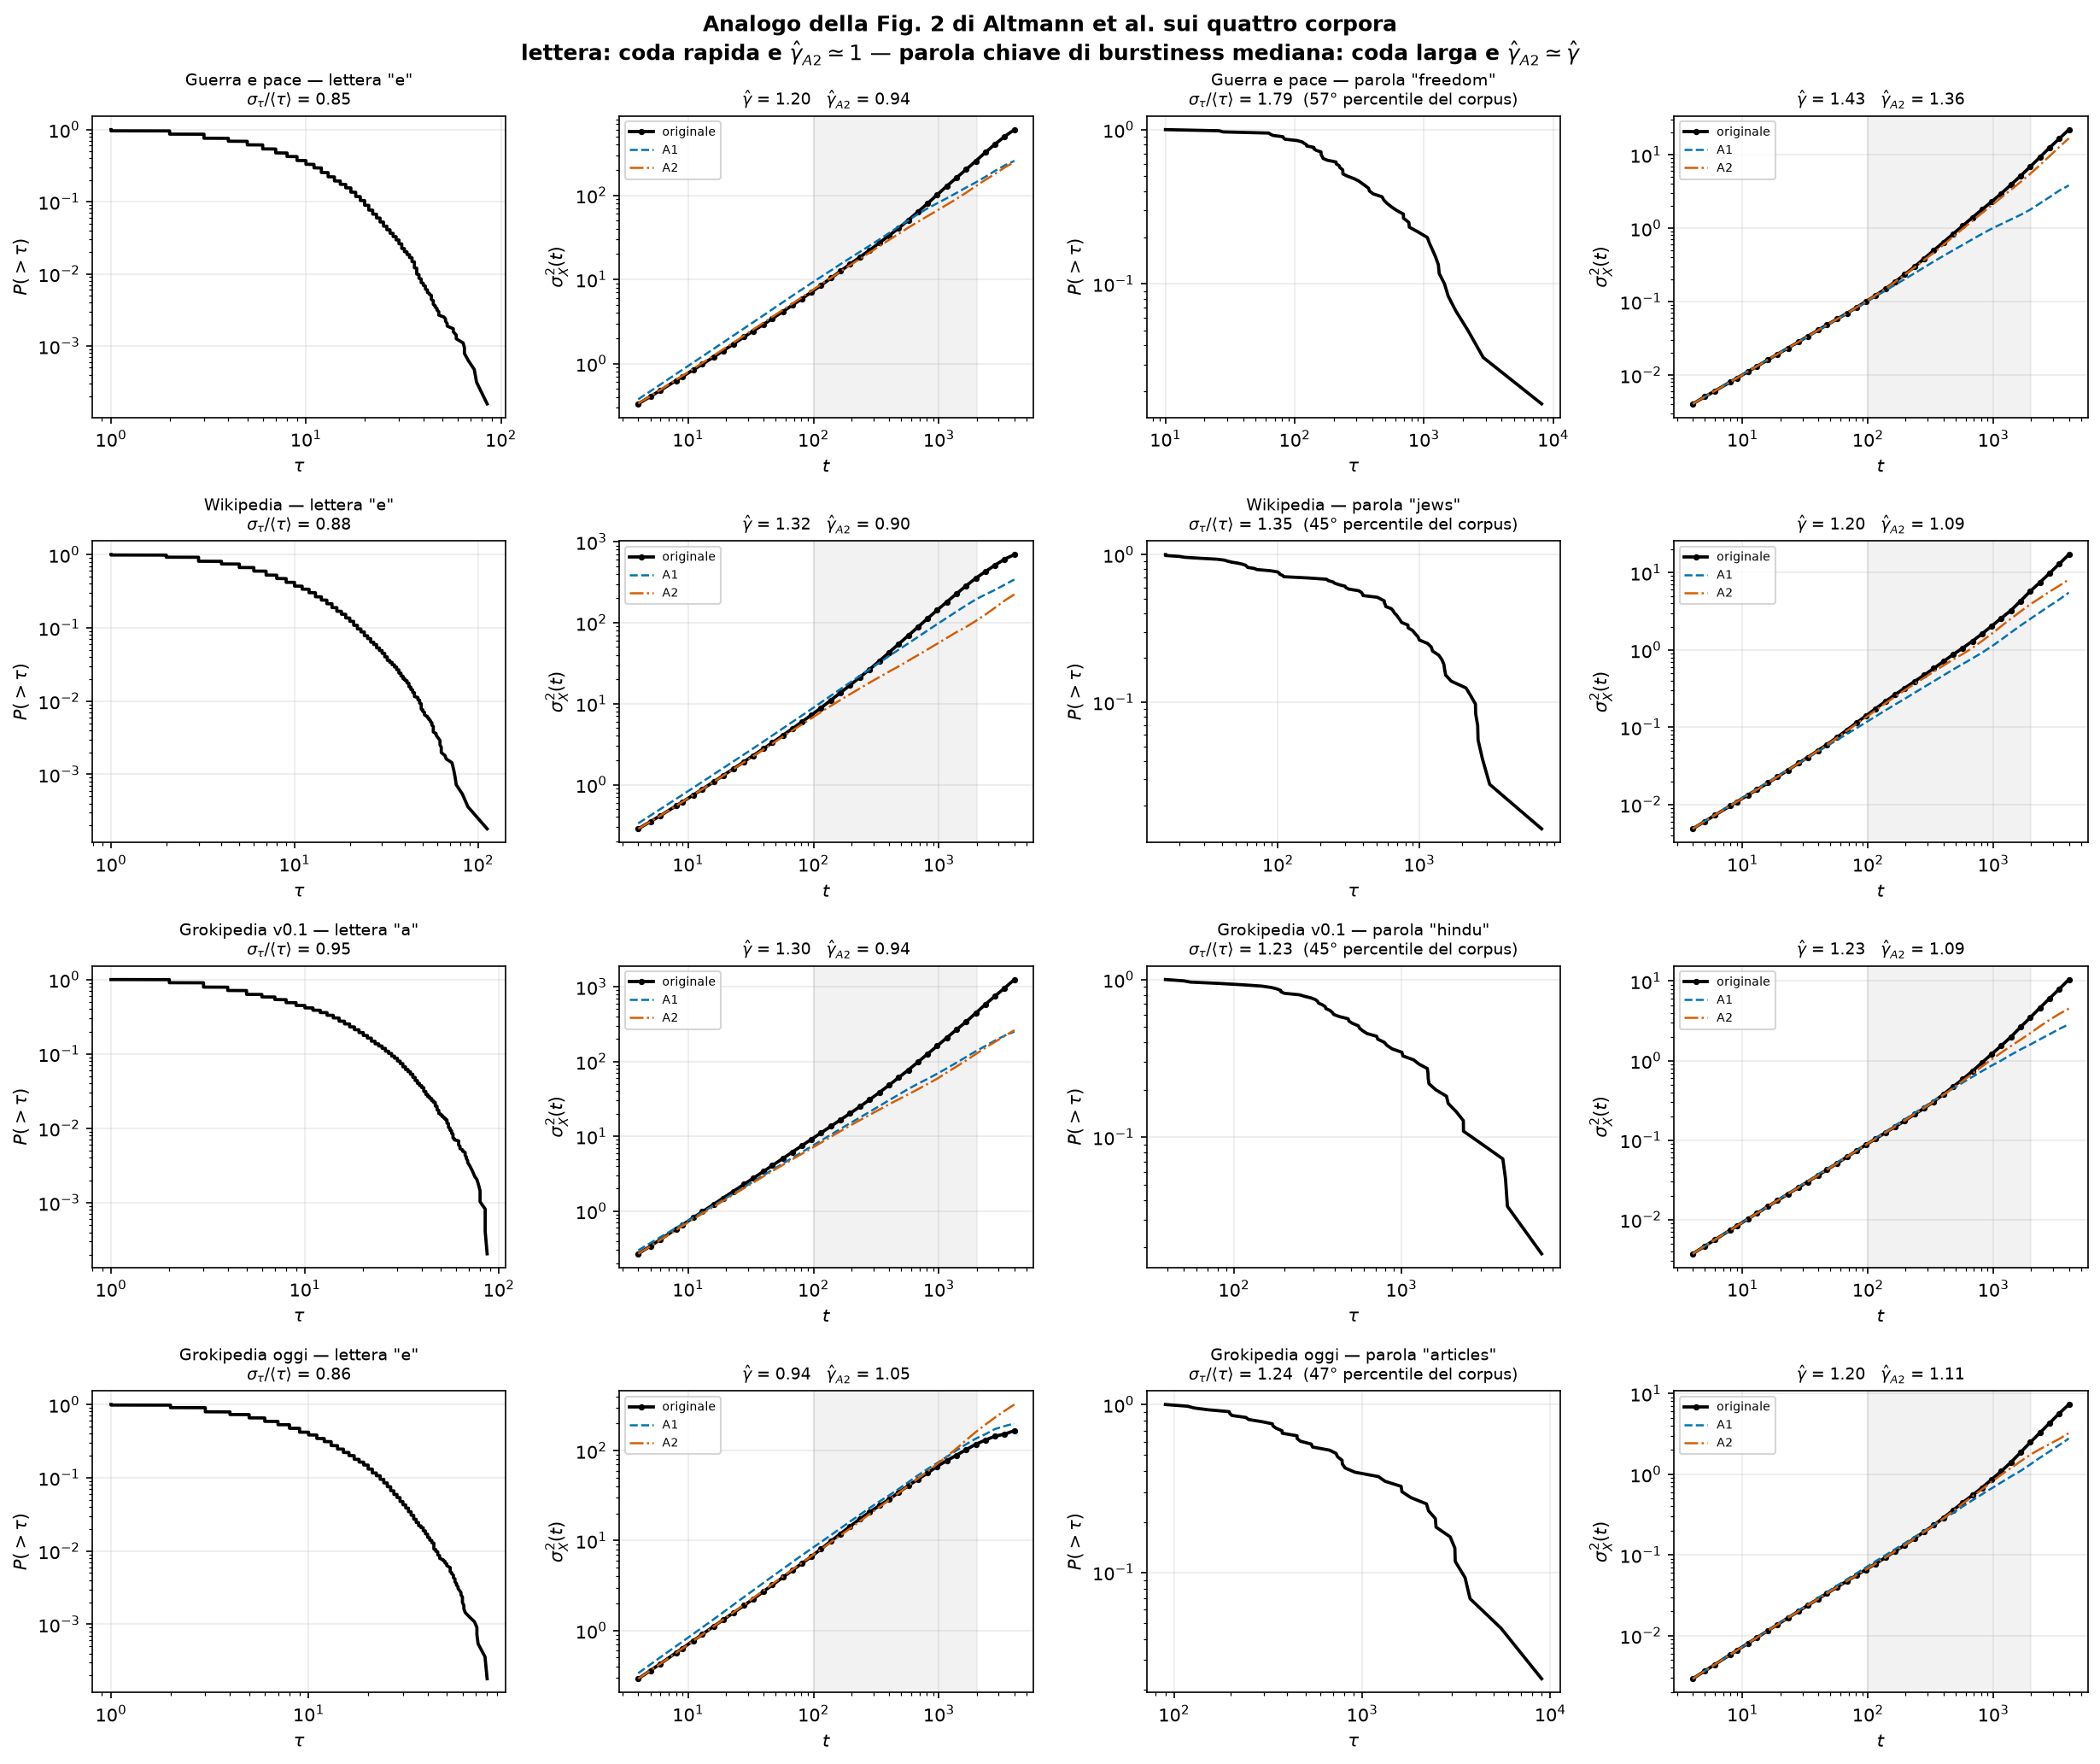
\includegraphics[width=\textwidth]{figure/cap5_altmann_fig2.png}
  \caption{Analogo della Figura~2 di~\cite{altmann2012} sui quattro corpora. Una
  riga per corpus; a sinistra la lettera più frequente del documento, a destra
  la parola chiave di burstiness mediana del corpus fra quelle con almeno
  \num{40} occorrenze, con il suo percentile indicato sopra il pannello. Per
  ciascuna, la distribuzione cumulata degli intervalli $P(>\tau)$ e la crescita
  della varianza del conteggio $\sigma_X^2(t)$, con le curve dei due null model
  del §\ref{sec:null} e la finestra di fit ombreggiata. La lettera ha coda
  rapida e $\hat\gamma_{A2} \simeq 1$; la parola di contenuto ha coda larga e
  $\hat\gamma_{A2}$ prossimo a $\hat\gamma$.}
  \label{fig:altmann-fig2}
\end{figure}

\paragraph{Il soggetto della voce non è una parola di contenuto.}
La parola chiave più ricorrente di un articolo enciclopedico, quella che il
criterio scartato sopra avrebbe selezionato, si comporta in modo opposto a
quello che il §\ref{sec:origini} prevede per il suo livello linguistico. Nella
voce \emph{Alexander the Great} di Wikipedia la parola \emph{alexander} ha
$\sigma_\tau/\langle\tau\rangle = 0.78$; in \emph{Sigmund Freud} di Grokipedia
\emph{freud} ha $0.72$. Sono valori sotto il limite poissoniano, cioè
distribuzioni \emph{più regolari del caso}, mentre la lettera \emph{e} negli
stessi testi dà $0.84$. Il confronto con la lettera non va però fatto sul valore
grezzo. Per un processo casuale in tempo discreto
$\sigma_\tau/\langle\tau\rangle$ non vale esattamente uno, ma tanto meno quanto
più corti sono gli intervalli: il null model A1, applicato alla stessa frequenza
della sequenza osservata, restituisce $0.95$ per la lettera \emph{e}, che ricorre
ogni dieci caratteri, e $1.00$ per una parola chiave, che ricorre ogni
duecento.

\paragraph{Il riferimento casuale dipende dalla frequenza.}
La ragione di quel $0.95$ è che gli intervalli sono numeri interi positivi. Se
le occorrenze sono collocate a caso con probabilità $f$ per carattere, la
distanza fra due consecutive è geometrica, e per la geometrica si ha
$\sigma_\tau/\langle\tau\rangle = \sqrt{1-f}$: il valore tende a uno solo nel
limite di eventi rari. Con $f = 1/10$, la frequenza della lettera \emph{e}, si
ottiene $0.949$; con $f = 1/200$, la frequenza tipica di una parola chiave,
$0.997$. Il valore poissoniano di riferimento non è dunque lo stesso ai due
livelli, ed è più basso proprio dove gli eventi sono più fitti. Confrontare
\emph{alexander} e la lettera \emph{e} sui valori grezzi significherebbe
attribuire alla struttura del testo una differenza che è invece un effetto
della sola frequenza.

Rapportando ciascuna misura al proprio valore casuale l'effetto si toglie, e
resta $0.78$ per \emph{alexander} contro $0.88$ per la lettera: il soggetto
della voce è più regolare di una lettera anche dopo aver tolto l'effetto della
frequenza, e la differenza fra i due, lungi dall'essere prodotta dalla
normalizzazione, ne esce accentuata.

\paragraph{Perché il soggetto si comporta così.}
La ragione è che in prosa enciclopedica il soggetto non è un tema fra altri,
che alterna presenza e assenza lungo il testo, ma il tema unico: compare come soggetto grammaticale di quasi ogni
periodo, e i suoi intervalli ereditano allora la statistica della lunghezza
delle frasi anziché quella dell'alternanza tematica. La verifica è diretta.
Nei sei articoli esaminati il soggetto ricorre una volta ogni $1.4$--$1.7$
frasi, con lo stesso valore in Wikipedia e in Grokipedia. I suoi intervalli sono
quindi lunghezze di frase, e ne ereditano la variabilità: le
lunghezze di frase di quegli articoli hanno
$\sigma_\tau/\langle\tau\rangle$ fra $0.33$ e $0.73$, e il soggetto della voce
si colloca poco sopra, fra $0.54$ e $0.78$, comunque sotto l'unità che
segnerebbe l'assenza di struttura. Per confronto, \emph{natásha} in un segmento
di \emph{Guerra e pace} ricorre una volta ogni $5.1$ frasi e ha
$\sigma_\tau/\langle\tau\rangle = 3.24$: lì la ricorrenza non segue il ritmo del
periodo ma l'alternanza delle scene.

Il soggetto della voce funziona quindi da marcatore sintattico e non semantico,
e la sua ricorrenza è governata dal ritmo del periodo, non dalla persistenza di
un argomento. Non è un difetto della misura ma un tratto del genere
enciclopedico, e va tenuto presente nel confrontare la burstiness lessicale fra
generi diversi: è la ragione per cui la parola mostrata nella
Figura~\ref{fig:altmann-fig2} viene scelta sulla mediana e non sul massimo.

% ---------------------------------------------------------------------
\section{Il divario si apre al livello lessicale}
\label{sec:appaiato}

L'appaiamento per titolo permette un test più stringente del confronto fra
medie. Confrontare la media di Wikipedia con quella di Grokipedia lascia
aperta l'obiezione che le due medie siano calcolate su argomenti diversi, e
che la differenza rifletta il contenuto anziché la scrittura. Il test appaiato
la chiude: per ciascuna delle \num{39} voci, che nei due corpora tratta lo
stesso argomento, si calcola la differenza fra il valore di Grokipedia e
quello di Wikipedia, e si verifica con il test dei ranghi segnati di Wilcoxon
che la mediana di quelle \num{39} differenze sia diversa da zero. Il test è
non parametrico, quindi non assume che le differenze siano distribuite
normalmente, assunzione che con \num{39} osservazioni e distribuzioni
asimmetriche non sarebbe difendibile.

Il test dà, per la versione attuale di Grokipedia,
$-0.167$ sulle parole chiave e $-0.010$ sulle lettere; ai due livelli intermedi
le differenze valgono $-0.037$ per le parole funzione e $-0.157$ per i controlli
appaiati, tutte con significatività inferiore a $10^{-2}$. La versione v0.1 dà
$-0.012$, $-0.039$, $-0.116$ e $-0.133$.

I quattro numeri vanno letti come una scala. Alle lettere Grokipedia e
Wikipedia distano un centesimo di unità di burstiness, cioè circa l'uno per
cento del valore misurato: a quel livello i due corpora sono, in pratica, lo
stesso testo. Alle parole funzione la distanza quadruplica, ma resta piccola in
termini relativi. Ai due livelli lessicali passa a circa sedici centesimi, oltre
un decimo del valore misurato e più di un ordine di grandezza sopra il livello
delle lettere.

La scala ha però un solo gradino, non tre. La differenza fra i livelli
sub-lessicali e quelli lessicali è netta; quella fra i due livelli lessicali non
esiste: $-0.157$ sui controlli a frequenza appaiata contro $-0.167$ sulle parole
chiave sono lo stesso numero. Il testo generato non perde dunque le parole di
contenuto più di quanto perda le altre parole della stessa frequenza. Ciò che i
dati sostengono è che riproduca le regolarità dei livelli bassi e abbassi
uniformemente la burstiness a livello di parola, non che perda selettivamente la
persistenza tematica.

\paragraph{Il divario alla lunghezza di controllo.}
\label{sec:robustezza-neff}
L'intera catena è stata ripetuta a $N_{\mathrm{eff}} = \num{80000}$ caratteri,
lunghezza a cui sopravvivono \num{35} delle \num{39} terne; per isolare
l'effetto della finestra, i valori a \num{60000} sono ricalcolati sulle stesse
\num{35}. Alle lettere e alle parole funzione il divario appaiato è stabile, da
$-0.010$ a $-0.011$ e da $-0.037$ a $-0.045$; ai due livelli lessicali si separa
in direzioni opposte, con i controlli appaiati da $-0.164$ a $-0.195$ e le parole
chiave da $-0.167$ a $-0.130$, quest'ultima con significatività che scende a
$p = 0.027$. Alla lunghezza maggiore il divario sulle parole chiave è dunque
\emph{minore} di quello sui controlli appaiati. Ciò che risulta robusto è il
salto dal livello sub-lessicale a quello lessicale; l'ulteriore crescita fino
alle parole chiave non lo è. Anche l'esponente di coda è instabile fra le due
lunghezze, da $2.19$ a $2.50$ su Grokipedia e da $2.37$ a $2.25$ su Wikipedia,
coerentemente con l'avvertenza del §\ref{sec:coda-risultati}.

La Figura~\ref{fig:altmann-fig3} riporta le stesse sequenze nel piano che
\cite{altmann2012} usa per la propria Figura~3: la burstiness in ascissa e
l'esponente di correlazione in ordinata, un punto per sequenza, con un simbolo
diverso per livello linguistico. La gerarchia vi si legge come una disposizione
spaziale: le lettere, gli spazi e le vocali si addensano in una colonna stretta
attorno a $\sigma_\tau/\langle\tau\rangle \simeq 0.5$, le parole funzione e i
controlli appaiati occupano la regione centrale, le parole chiave si spingono a
destra e in alto. È la stessa gerarchia dei paragrafi precedenti, vista tutta
insieme invece che un livello alla volta.

Il piano rende però visibile anche una proprietà che i confronti per livello
non mostrano, e che è l'osservazione centrale di quel lavoro: l'angolo in
basso a destra è vuoto. Non esistono, cioè, sequenze molto \emph{bursty} e
insieme poco correlate. Sui quattro corpora di questa tesi la regolarità si
quantifica così: delle $451$ sequenze con $\sigma_\tau/\langle\tau\rangle >
1.5$, soltanto $17$, il $3.8\%$, hanno $\hat\gamma < 1.1$, e fra quelle con
burstiness superiore a $2$ l'esponente non scende mai sotto $1.05$. L'angolo
opposto, invece, è popolato: delle $3500$ sequenze sotto il valore poissoniano
$\sigma_\tau/\langle\tau\rangle = 1$, il $15.9\%$ ha $\hat\gamma > 1.2$.

L'asimmetria fra i due angoli è la firma di una relazione a senso unico. La
burstiness produce correlazione, come mostra la~\eqref{eq:eq4}, e una sequenza
con vuoti lunghi non può quindi risultare scorrelata; il viceversa non vale,
perché la correlazione può venire anche dall'ordine degli intervalli e
manifestarsi senza alcuna coda pesante. La correlazione di rango fra le due
quantità è positiva e significativa in tutti e quattro i corpora, da $+0.22$ su
Wikipedia a $+0.36$ sul romanzo. Il meccanismo descritto in~\cite{altmann2012}
sui romanzi si ritrova dunque identico nella prosa enciclopedica e in quella
generata, ed è un risultato indipendente dal divario misurato sopra: riguarda
come le due grandezze si legano fra loro, non quanto valgano.

\begin{figure}[htbp]
  \centering
  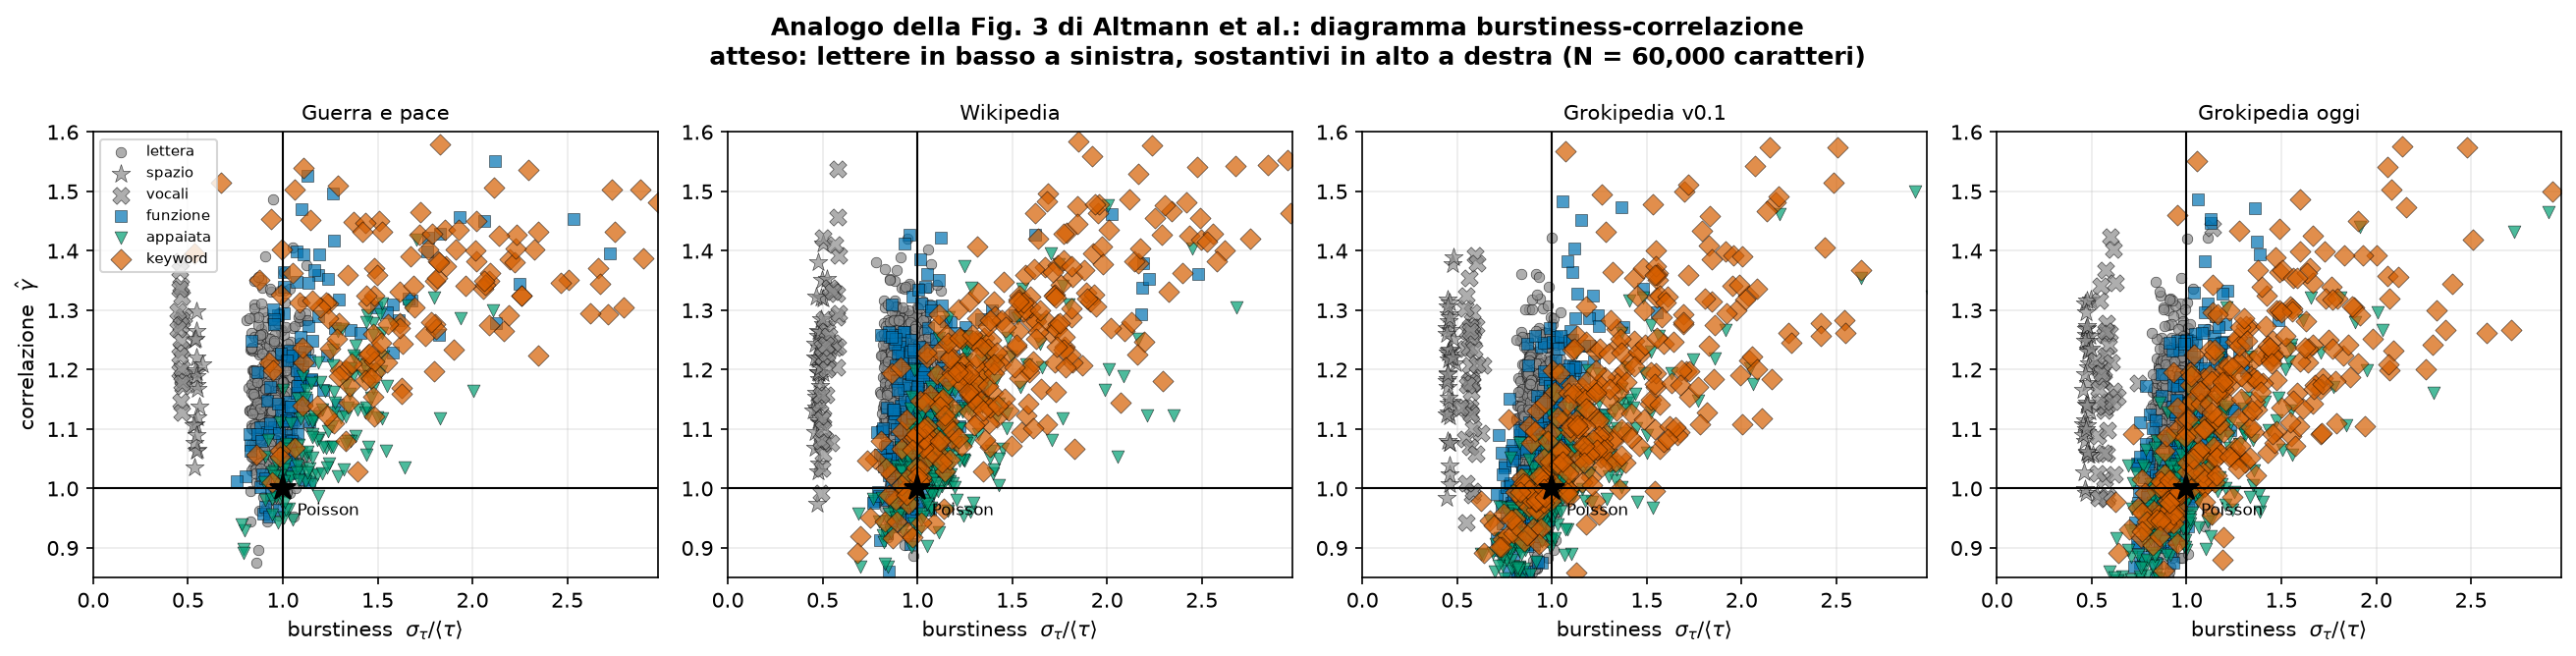
\includegraphics[width=\textwidth]{figure/cap5_altmann_fig3.png}
  \caption{Analogo della Figura~3 di~\cite{altmann2012}: diagramma
  burstiness--correlazione sui quattro corpora, un punto per sequenza. Oltre ai
  quattro livelli usati nel resto del capitolo sono riportati i due livelli
  sub-lessicali tenuti come diagnostica, gli spazi e le vocali. Le linee nere
  segnano il processo di Poisson,
  $\sigma_\tau/\langle\tau\rangle = 1$ e $\hat\gamma = 1$. L'angolo in basso a
  destra è praticamente vuoto in tutti e quattro i corpora: sequenze molto
  bursty e insieme poco correlate non si osservano.}
  \label{fig:altmann-fig3}
\end{figure}

\paragraph{I due quadranti che restano.} La lettura del piano fatta finora
riguarda la diagonale: l'angolo in basso a destra vuoto e quello in alto a
sinistra popolato. Gli altri due separano però i corpora meglio di qualunque
media, e la Figura~\ref{fig:quadranti} li riporta separatamente. Fra le parole
chiave, l'angolo in alto a destra è la posizione canonica
di~\cite{altmann2012}, quella in cui la sequenza è insieme bursty e correlata.
Vi ricade il $91.4\%$ delle sequenze di \emph{Guerra e pace} e l'$87.5\%$ di
quelle di Wikipedia, ma solo il $74.0\%$ di Grokipedia v0.1 e il $77.3\%$
della versione attuale. La differenza finisce quasi interamente nell'angolo
opposto, in basso a sinistra, dove la parola è più regolare di un processo di
Poisson e insieme priva di correlazione a lungo raggio: $0\%$ sul romanzo,
$5.1\%$ su Wikipedia, $15.4\%$ su Grokipedia v0.1 e $14.3\%$ sulla versione
attuale. Una parola chiave generata su sette si trova dunque nell'angolo
opposto a quello canonico, contro una su venti in Wikipedia. Il test appaiato
sulle \num{39} voci conferma che non è un effetto di composizione del
campione: la quota di parole chiave in basso a sinistra cresce in $21$ e $22$
voci su $39$, con differenza mediana $+0.143$ e $p < 10^{-3}$ per entrambe le
versioni.

Due controlli escludono le spiegazioni strumentali. Il null model A1
restituisce $\hat\gamma = 0.983$ in tutti e quattro i corpora, identico alla
terza cifra, quindi la soglia $\hat\gamma = 1$ non è tarata diversamente da un
corpus all'altro; il valore calibrato non è però esattamente uno, cosicché la
soglia è lievemente generosa verso il lato correlato, allo stesso modo per
tutti. E la quota di parole in basso a sinistra resta più alta in Grokipedia
dentro quattro fasce di frequenza su cinque, da $0.159$ contro $0.050$ per le
parole con $26$--$35$ occorrenze a $0.303$ contro $0.076$ per quelle con più di
$80$. Fa eccezione la fascia più bassa, $15$--$25$ occorrenze, dove il rapporto
si inverte, $0.065$ contro $0.200$; lì però le parole chiave di Wikipedia sono
dieci in tutto e la quota è stimata su di esse. Il divario non dipende quindi
dal fatto che le parole chiave di Wikipedia siano più frequenti, salvo nella
fascia in cui il confronto ha meno appoggio.

Guardare dentro il quadrante non rivela più un gruppo omogeneo. Separando le
parole che compaiono nel titolo della voce dalle altre, le $14$ di Wikipedia si
dividono a metà, e le $39$ di Grokipedia si dividono in $18$ soggetti di voce e
$21$ altre parole, prevalentemente aggettivi generici: \emph{economic} in cinque
voci, \emph{military} in tre, \emph{urban} in due. Sono concentrazioni modeste,
e soprattutto non sono più quelle che la lista di parole funzione originaria
lasciava passare: con quella lista, il quadrante conteneva \emph{like} in dodici
voci, \emph{amid} in nove e \emph{including} in sei, cioè i connettivi che
costituiscono il vizio stilistico più evidente del testo generato. Quei termini
sono ora classificati come parole funzione, che è ciò che sono, e il
§\ref{sec:effetto-stoplist} misura quanto la loro presenza fra le parole chiave
alterasse i risultati.

\begin{figure}[htbp]
  \centering
  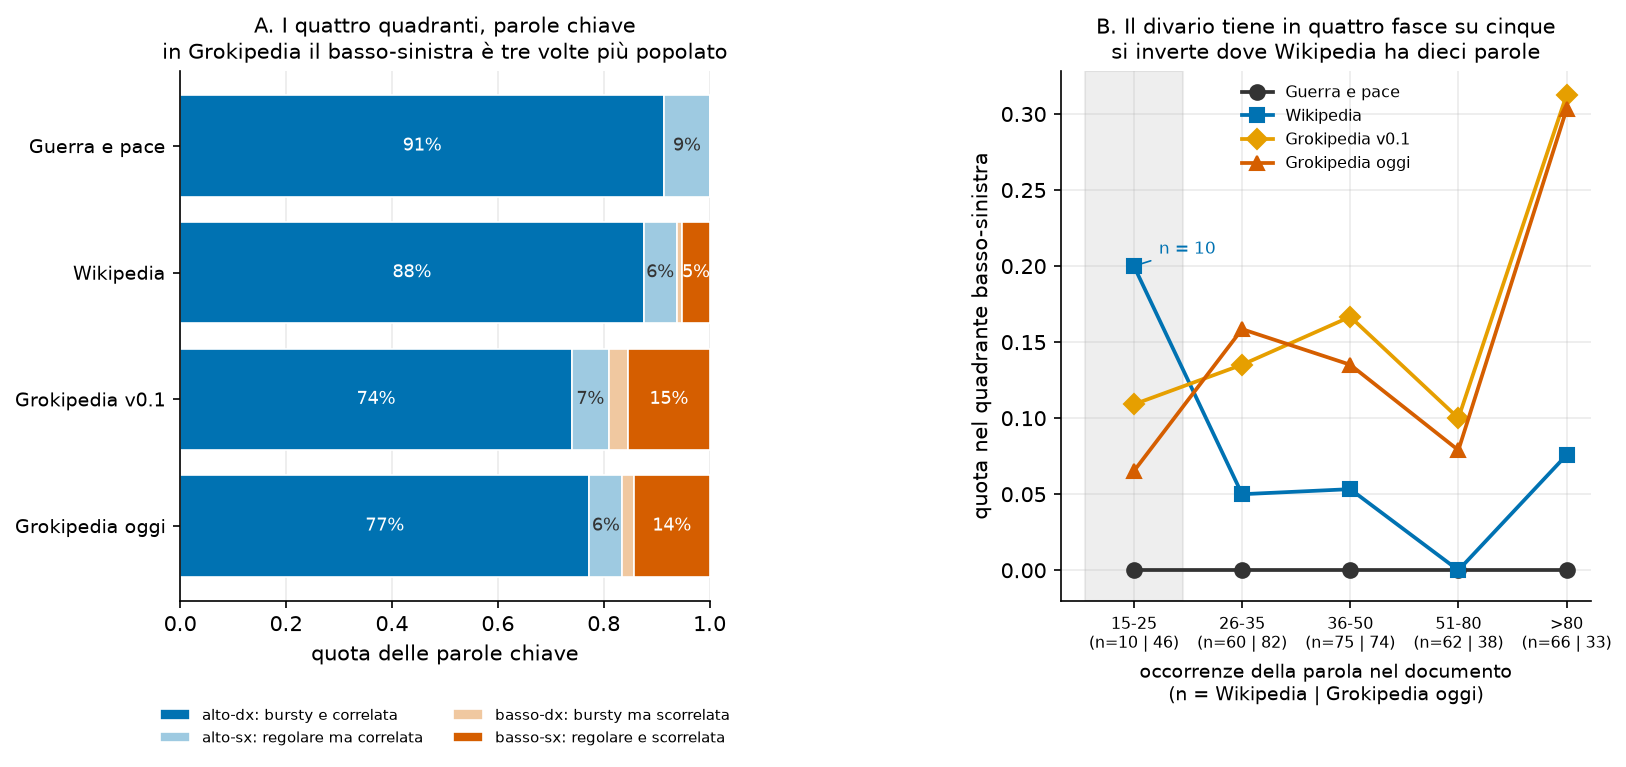
\includegraphics[width=\textwidth]{figure/cap5_quadranti.png}
  \caption{Lettura per quadranti del piano della
  Figura~\ref{fig:altmann-fig3}, sulle sole parole chiave. A: composizione per
  quadrante, un corpus per riga; le quote sotto il $5\%$ non sono etichettate. B:
  quota di parole chiave nel quadrante in basso a sinistra, separando le parole
  per numero di occorrenze nel documento; sotto ciascuna fascia è indicato
  quante parole chiave vi cadono in Wikipedia e in Grokipedia. Il divario tiene
  in quattro fasce su cinque e si inverte nella più bassa, dove Wikipedia ne ha
  dieci in tutto e la fascia è ombreggiata per segnalarlo.}
  \label{fig:quadranti}
\end{figure}

\paragraph{Un effetto di scala da neutralizzare.} Le voci di Grokipedia hanno
frasi sensibilmente
più lunghe di quelle di Wikipedia: $4.38$ frasi ogni mille caratteri contro
$6.92$. Poiché in questo capitolo il tempo è contato in caratteri, la scala
degli intervalli $\tau$ non è la stessa nei due corpora, e un testo con frasi
più lunghe tende ad avere intervalli più lunghi anche a parità di struttura
tematica. Il coefficiente di variazione è un rapporto e non risente di una
dilatazione uniforme dell'asse, ma la dilatazione qui non è uniforme, perché
agisce solo sui livelli definiti su unità linguistiche. Il
§\ref{sec:entropia-intervalli} introduce la misura che elimina il problema;
fino a quel punto il divario va considerato provvisorio.

Il riferimento letterario, infine, non è appaiato per argomento con nessuno dei
tre corpora enciclopedici: entra nei confronti come livello medio e non nei test
appaiati.

% ---------------------------------------------------------------------
\section{Quale meccanismo genera la correlazione}
\label{sec:decomposizione}

Sapere che un testo ha correlazioni a lungo raggio non dice da dove esse
vengano. Il §\ref{sec:null} ha introdotto i due null model che separano le due
origini possibili e la quota di burstiness $q$ della~\eqref{eq:quota}, che vale
circa uno quando la correlazione è interamente spiegata dalla distribuzione
degli intervalli, e circa zero quando è invece l'ordine in cui le occorrenze si
susseguono a produrla.

Il primo pannello della Figura~\ref{fig:decomposizione} riporta $q$ ai quattro
livelli. Sulle lettere il valore è negativo in tutti e quattro i corpora, da
$-0.06$ su Wikipedia a $-0.19$ su Grokipedia v0.1: le lettere sono correlate,
come mostra il $\hat\gamma$ maggiore di uno, ma non sono \emph{bursty}, e la
correlazione viene interamente dall'ordine. Sulle parole chiave il valore sale a
$0.89$ sul romanzo, $0.77$ su Wikipedia, $0.70$ sulla v0.1 e $0.74$ sulla
versione attuale di Grokipedia: qui quasi tutta la correlazione è già contenuta nella
distribuzione degli intervalli. I due livelli intermedi interpolano fra i due
regimi in modo ordinato.

La dissociazione fra il livello dei caratteri e quello del contenuto, che
in~\cite{altmann2012} è osservata su romanzi, si ritrova quindi identica nella
prosa enciclopedica e anche nella prosa generata. Il secondo pannello mostra la
stessa cosa in termini di esponenti: le curve piene sono $\hat\gamma$ e quelle
tratteggiate $\hat\gamma_{A2}$, e la distanza verticale fra le due è il
contributo dell'ordine delle occorrenze. Sulle lettere le due curve sono
separate e la tratteggiata sta all'unità; sulle parole chiave si avvicinano e
salgono insieme.

I valori dei tre corpora enciclopedici sono però troppo vicini perché la
differenza sia interpretabile: fra Wikipedia e Grokipedia vale $0.03$ alla
lunghezza di lavoro e cambia segno a quella di controllo del
§\ref{sec:robustezza-neff}. I dati non consentono quindi di attribuire ai due
corpora un'origine diversa della correlazione, ma soltanto un'intensità diversa.

Sulla riga dei controlli appaiati per Grokipedia, infine, la quota è stimabile
solo su $6$ documenti su $39$ per la versione v0.1 e su $8$ per quella
attuale. La ragione non è un difetto della stima ma la grandezza stessa: $q$
ha $\hat\gamma - 1$ al denominatore, e viene calcolata soltanto dove quel
denominatore supera $0.05$, perché sotto quella soglia il rapporto è dominato
dall'errore. A quel livello i documenti di Grokipedia hanno $\hat\gamma$
mediano pari a $1.003$ per la v0.1 e $1.015$ per la versione attuale, contro
$1.091$ di Wikipedia: le loro sequenze di controllo sono essenzialmente
scorrelate, e non c'è alcuna correlazione da decomporre nelle due origini.
L'esclusione è quindi essa stessa un dato, perché è il livello in cui il testo
generato si avvicina di più al caso, ma il valore di $q$ che sopravvive sui
pochi documenti restanti riguarda proprio quelli in cui una correlazione c'è,
e non va letto come una misura del corpus.

\begin{figure}[htbp]
  \centering
  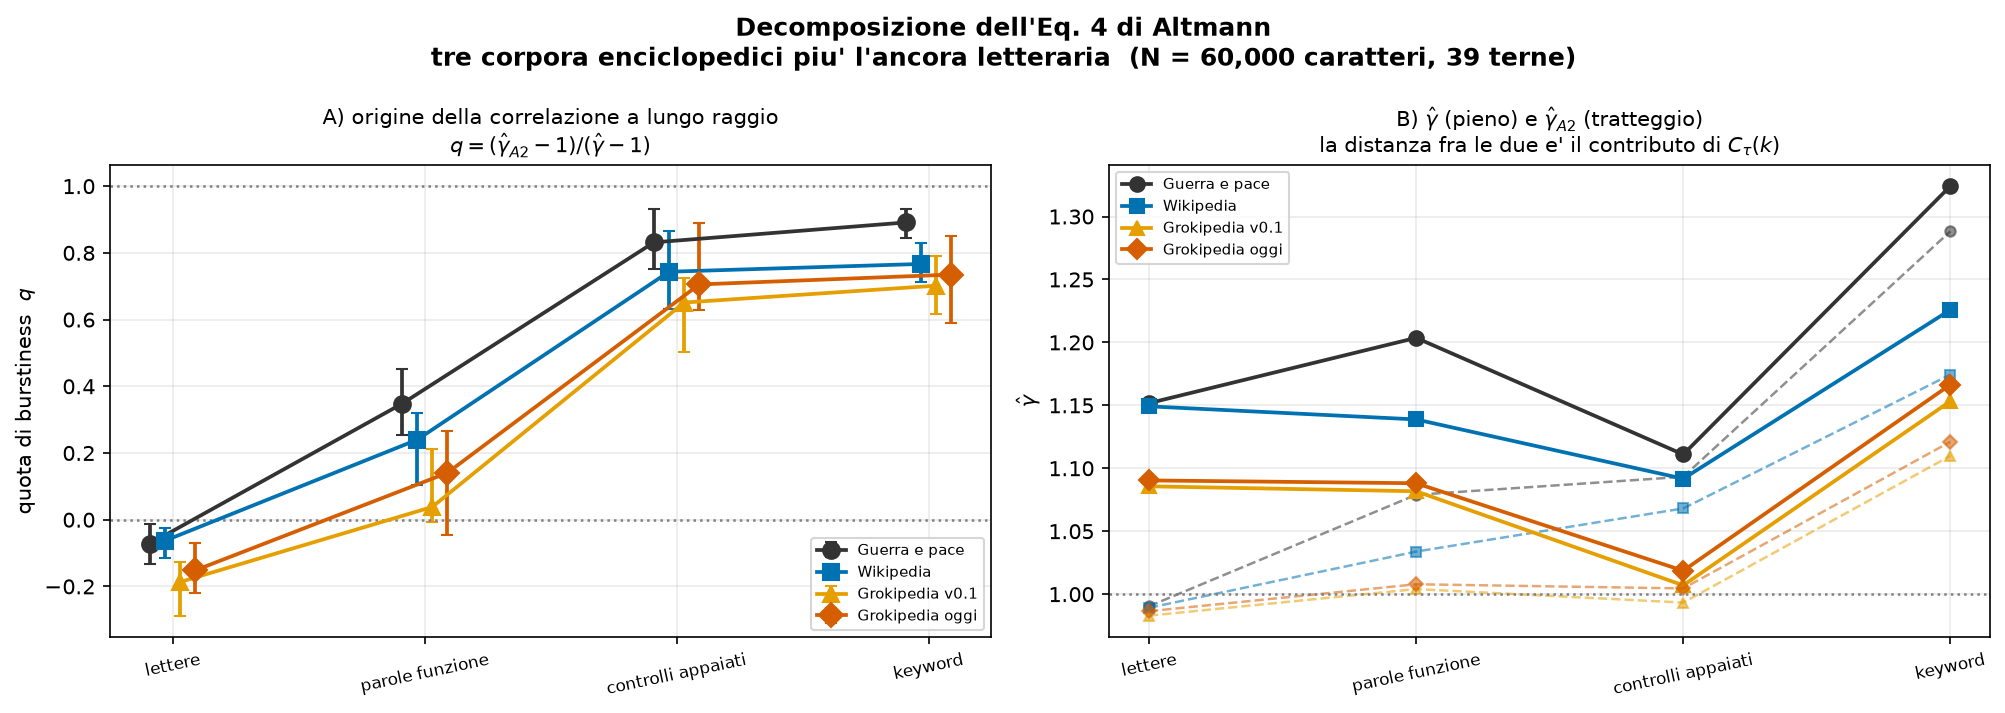
\includegraphics[width=\textwidth]{figure/cap5_decomposizione_eq4.png}
  \caption{Decomposizione della correlazione nelle sue due origini. A: quota
  $q$ della~\eqref{eq:quota} ai quattro livelli linguistici, con intervalli di
  confidenza; $q \simeq 0$ indica correlazione dovuta all'ordine delle
  occorrenze, $q \simeq 1$ correlazione dovuta alla distribuzione degli
  intervalli. B: esponente $\hat\gamma$ (linea piena) e $\hat\gamma_{A2}$
  (tratteggiata) agli stessi livelli; la distanza fra le due curve è il
  contributo della correlazione fra intervalli successivi.}
  \label{fig:decomposizione}
\end{figure}

% ---------------------------------------------------------------------
\section{La coda della distribuzione degli intervalli}
\label{sec:coda-risultati}

Il §\ref{sec:coda} ha osservato che la relazione fra esponente di coda e
esponente di correlazione, nella forma in cui compare in~\cite{altmann2012},
presuppone una distribuzione degli intervalli di cui la coda non viene misurata
ma assunta. Qui la coda viene stimata direttamente, adottando il modello
troncato
\begin{equation}
  p(\tau) \;\sim\; \tau^{-\mu}\,e^{-\tau/\tau_c}
  \label{eq:coda-troncata}
\end{equation}
e determinando $\mu$ e $\tau_c$ per massima verosimiglianza, con intervalli di
confidenza di profilo.

L'analisi della coda comprende, oltre ai quattro livelli usati nel resto del
capitolo, due livelli sub-lessicali aggiuntivi tenuti come diagnostica, le
vocali e gli spazi, per un totale di ventiquattro celle. Il primo risultato
riguarda la forma stessa della distribuzione: il confronto di verosimiglianza
fra la~\eqref{eq:coda-troncata} e una legge di potenza pura rifiuta
quest'ultima in tutte e ventiquattro, con significatività numericamente
indistinguibile da zero. La coda esiste, ma è tagliata.

Il primo pannello della Figura~\ref{fig:coda} riporta $\mu$ ai quattro livelli.
La banda verde segna la regione $2 < \mu < 3$ entro cui la~\eqref{eq:eq8} è
derivata assumendo una legge di potenza pura. Che le stime vi cadano dentro o
fuori non dice nulla sulla convergenza dei momenti: nella
~\eqref{eq:coda-troncata} il taglio li rende finiti per qualunque $\mu$, e il
rifiuto della potenza pura in tutte e ventiquattro le celle toglie il
presupposto sotto cui la banda avrebbe quel significato. Resta un riferimento
utile perché è la regione in cui il paper colloca il proprio valore assunto.
I simboli grigi segnalano le celle in cui il fit degenera in un
esponenziale puro e $\mu$ non è interpretabile, e le linee di collegamento le
saltano. Sono sette celle su sedici: tutti e quattro i corpora sul livello delle
lettere, e i tre corpora enciclopedici su quello delle parole funzione.

Alle parole funzione il romanzo è l'unico dei quattro il cui fit non degenera,
con $\tau_c = 5.3$ contro $1.7$--$1.9$: le sue parole funzione conservano un
tratto di coda a legge di potenza che negli altri tre corpora non esiste, e a
quel livello il coefficiente di variazione dà lo stesso quadro, $1.19$ contro
valori fra $0.97$ e $1.03$ indistinguibili da un processo di Poisson.

Sarebbe naturale leggerlo come una differenza di genere, e il controllo non lo
conferma. Ripetendo la stessa procedura sui tre romanzi inglesi impiegati come
controllo in questo capitolo, il fit sulle parole funzione degenera su
\emph{Moby Dick} ($\tau_c = 1.7$, esattamente il valore dei corpora
enciclopedici) e su \emph{David Copperfield} ($\tau_c = 2.8$), e sopravvive per
poco su \emph{Middlemarch} ($\tau_c = 3.2$); il coefficiente di variazione dà
$1.03$, $1.09$ e $1.08$, cioè valori compresi fra Wikipedia e
\emph{Guerra e pace} e nel primo caso identici a quelli enciclopedici. A questo
livello l'eccezione è quindi del testo e non del genere, come il
§\ref{sec:tre-corpora} osserva anche sul livello delle parole chiave. Il confronto fra i quattro
corpora resta perciò leggibile soltanto sulle parole chiave, dove i valori
stanno fra $1.76$ e $2.37$; sui controlli appaiati tutti e quattro i fit sono al
limite della degenerazione e gli intervalli di confidenza superano l'unità di
ampiezza.

Il confronto con~\cite{altmann2012} chiude qui un cerchio. In quel lavoro $\mu$
non viene stimato ma assunto: per costruire il limite inferiore di $\hat\gamma$
della propria Figura~3 gli autori adottano il valore $\mu = 2.4$. La stima
diretta condotta qui lo colloca dentro l'intervallo di confidenza di tutti e tre
i corpora enciclopedici, e a tre centesimi dal valore centrale di Wikipedia. Il
parametro che quel lavoro doveva postulare risulta dunque misurabile, e il
valore postulato corretto. Il confronto è legittimo perché $\mu$ designa in
entrambi i casi la pendenza della coda nella regione in cui la legge di potenza
vale; ciò che cambia è che qui quella regione è delimitata da un $\tau_c$
stimato anziché estesa all'infinito, e il capoverso seguente misura quanto la
differenza di modello sposti il numero.

Il corpus letterario fa eccezione, con $\mu = 1.76$ e intervallo di confidenza
$[1.40, 2.08]$, e su questo servono due precisazioni, perché il valore cade
sotto la banda $2 < \mu < 3$ entro cui la~\eqref{eq:eq8} è derivata. La prima
è che non è una particolarità di \emph{Guerra e pace}: ripetendo l'intera
procedura su tre altri romanzi inglesi, segmentati e misurati allo stesso
modo, si ottiene $1.51$ su \emph{Moby Dick}, $2.10$ su \emph{Middlemarch} e
$1.96$ su \emph{David Copperfield}, tutti sotto il valore di Wikipedia a ogni
quantile di $x_{\min}$ dall'ottantesimo in su. È un tratto della prosa
letteraria, non del testo scelto, ed è lo stesso fatto che il coefficiente di
variazione registra come burstiness massima: coda più pesante significa
esponente più piccolo.

La seconda è che il valore dipende dal modello con cui lo si stima. Sotto il
modello troncato adottato qui la banda $2 < \mu < 3$ non ha ruolo, perché il
taglio rende media e varianza finite per qualunque $\mu$; sotto il modello a
potenza pura, che è quello di~\cite{altmann2012}, lo stimatore di massima
verosimiglianza sugli stessi dati dà $2.49$ per il corpus letterario, dentro la
banda e a nove centesimi dal valore assunto nel paper. I due numeri non sono in
conflitto: descrivono la stessa coda sotto ipotesi diverse, e la scelta fra le
due è decisa dal rapporto di verosimiglianza, che rifiuta la potenza pura. La
misura non contraddice dunque il valore postulato in quel lavoro; ne circoscrive
il modello.

\begin{figure}[htbp]
  \centering
  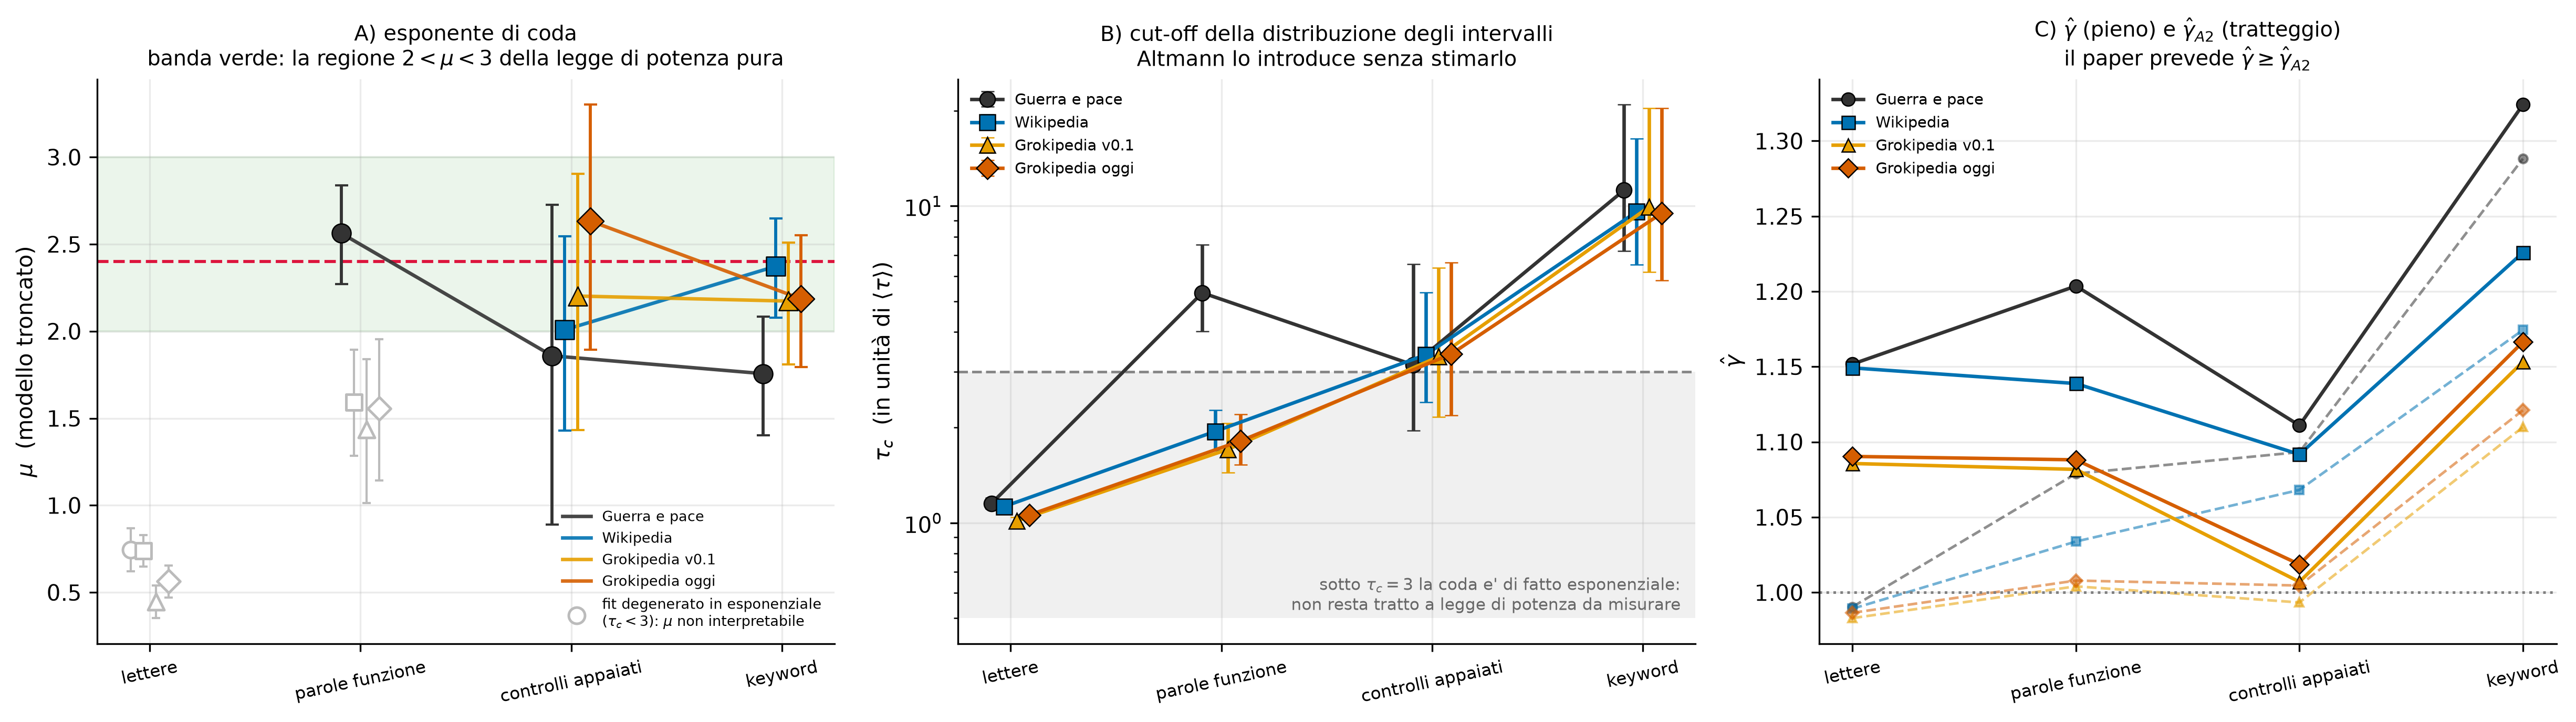
\includegraphics[width=\textwidth]{figure/cap5_esponente_coda.png}
  \caption{Stima diretta della coda della distribuzione degli intervalli. A:
  esponente $\mu$ della~\eqref{eq:coda-troncata} ai quattro livelli, con
  intervalli di confidenza di profilo; la banda verde è la regione $2<\mu<3$ in
  cui è derivata la~\eqref{eq:eq8} per la legge di potenza pura, mentre sotto il
  modello troncato adottato qui i momenti restano finiti per qualunque $\mu$ e
  la banda va letta come riferimento alla letteratura; i simboli grigi sono le
  celle in cui il fit degenera in un esponenziale e $\mu$ non è interpretabile,
  che le linee di collegamento saltano. B: cut-off
  $\tau_c$ agli stessi livelli, in unità dell'intervallo medio e con intervalli
  di confidenza di profilo; sotto la soglia tratteggiata non resta tratto a legge
  di potenza da misurare. C: $\hat\gamma$ (pieno) contro $\hat\gamma_{A2}$
  (tratteggiato) ai quattro livelli. La~\eqref{eq:disug1} è rispettata in tutte
  le celle: la curva piena sta sempre sopra la tratteggiata.}
  \label{fig:coda}
\end{figure}

\paragraph{Perché $\mu$ non serve a confrontare i corpora.}
I quattro valori non vanno però usati per ordinare i corpora, e la
Figura~\ref{fig:verosimiglianza} mostra perché: $\mu$ e $\tau_c$ sono
fortemente correlati, cosicché le regioni di confidenza congiunte sono creste
allungate anziché ellissi compatte e quelle dei tre corpora enciclopedici si
sovrappongono quasi interamente. A ciò si aggiunge la dipendenza dal punto in
cui si decide che la coda cominci: spostando $x_{\min}$ dal settantacinquesimo
al novantacinquesimo percentile $\mu$ passa da $1.65$ a $2.63$ su Wikipedia, una
variazione maggiore di ogni differenza fra corpora, e le curve si incrociano.

Di questa analisi non resta perciò un ordinamento fra corpora. Restano due
risultati, entrambi insensibili alla posizione esatta lungo la cresta: la legge
di potenza pura è rifiutata ovunque, e il cut-off cresce in modo ordinato
salendo nella gerarchia linguistica. Il cut-off è previsto
da~\cite{altmann2012} come conseguenza della discesa lungo quella stessa
gerarchia, e la sua esistenza è qui verificata invece che assunta.

\begin{figure}[htbp]
  \centering
  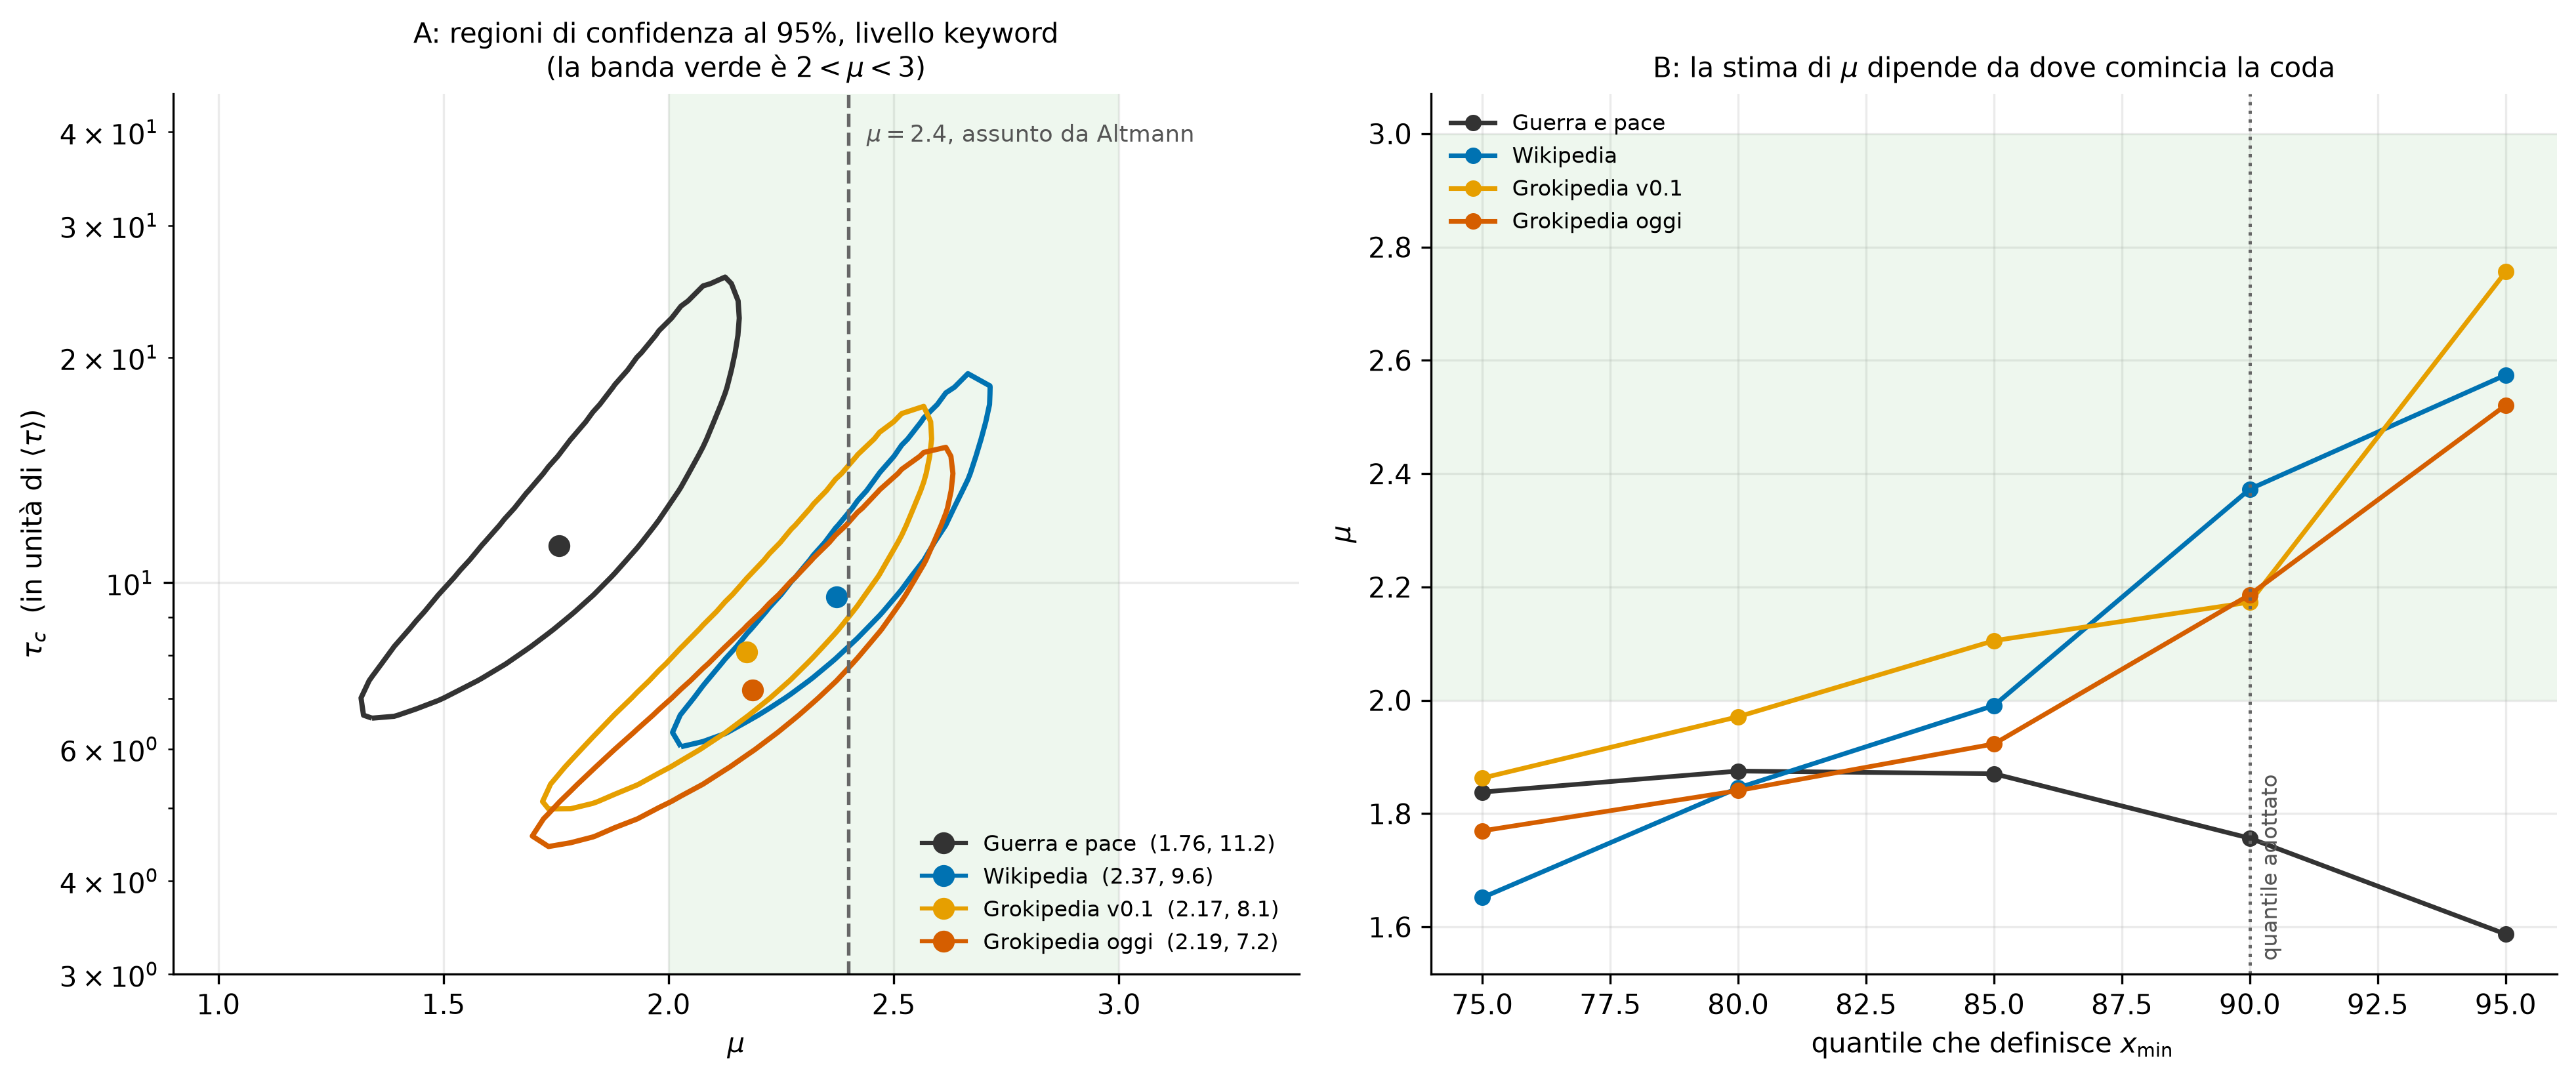
\includegraphics[width=\textwidth]{figure/cap5_verosimiglianza_coda.png}
  \caption{Perché l'esponente di coda non discrimina fra i corpora. A: regioni
  di confidenza congiunte al $95\%$ nel piano $(\mu, \tau_c)$ sul livello delle
  parole chiave, con $x_{\min}$ al novantesimo percentile; l'allungamento delle
  regioni è la correlazione fra i due parametri, e la linea tratteggiata è il
  valore $\mu = 2.4$ assunto in~\cite{altmann2012}. B: stima di $\mu$ al variare
  del quantile che definisce $x_{\min}$; le quattro curve si incrociano, cosicché
  l'ordinamento fra corpora dipende da quella scelta.}
  \label{fig:verosimiglianza}
\end{figure}

\paragraph{Il cut-off e la finestra di osservazione.} Il secondo pannello
della Figura~\ref{fig:coda} riporta $\tau_c$ ai quattro livelli, con
intervalli di confidenza di profilo. È l'altra metà di ciò
che~\cite{altmann2012} introduce senza stimare: il cut-off vi compare come
conseguenza necessaria della discesa nella gerarchia, ma non gli viene mai
assegnato un valore. Cresce in modo ordinato salendo nella gerarchia: circa
$1.1$ volte l'intervallo medio sulle lettere, dove la coda è di fatto già
esponenziale, $3.2$--$3.4$ sui controlli appaiati e $9.5$--$11.2$ sulle parole
chiave. La separazione fra i due livelli superiori è netta. Fra i quattro
corpora, invece, gli intervalli di confidenza si sovrappongono ampiamente:
neppure il cut-off ordina i corpora, e la sola cella in cui la separazione è
significativa è quella delle parole funzione del romanzo, discussa sopra.

Anche $\tau_c$ va poi letto come descrittore relativo alla lunghezza di analisi.
Ripetendo la stima sul romanzo a lunghezze crescenti, da \num{30000} a
\num{480000} caratteri, $\tau_c$ passa da $13.5$ a $94.7$: un fattore sette a
fronte di un fattore sedici sulla finestra, con un andamento non monotono che
scende prima di risalire. Il taglio non è dunque un puro artefatto, perché non
scala proporzionalmente alla finestra, ma non è nemmeno una lunghezza intrinseca
del testo. Sulla stessa serie $\mu$ si stabilizza attorno a $2.0$ alle finestre
maggiori, contro l'$1.76$ misurato alla lunghezza di lavoro: entrambi i
parametri descrivono la coda \emph{a quella lunghezza}, coerentemente con la
regola del §\ref{sec:lunghezza}.

\paragraph{Lo stimatore di Hill.} Dà sistematicamente valori più alti, $2.49$ sul
romanzo contro $1.76$ e circa $3.0$ sugli altri tre corpora contro
$2.2$--$2.4$, perché assume una legge di potenza pura su tutta la coda.
L'assenza di un plateau nel suo grafico diagnostico è ciò che ha motivato
l'adozione del modello troncato, e i suoi valori sono riportati solo a quel
titolo.

% ---------------------------------------------------------------------
\section{Entropia degli intervalli}
\label{sec:entropia-intervalli}

L'effetto di scala dichiarato nel §\ref{sec:appaiato} richiede una misura che
non risenta della lunghezza media delle frasi. È la ragione per cui il
§\ref{sec:entropia-intervalli-def} ha introdotto l'entropia degli intervalli
$J$ della~\eqref{eq:entropia-intervalli}: il logaritmo la rende invariante per
dilatazione dell'asse, cosicché frasi mediamente più lunghe non la spostano, e
la sottrazione del termine poissoniano ne cancella il bias. La grandezza è
risultata calcolabile su \num{5343} sequenze su \num{5617}, il $95\%$ del
totale.

\paragraph{Perché la misura è legittima.}
Trattandosi di una grandezza introdotta qui, la sua adozione va giustificata su
quello che fa e non su un precedente. I due ingredienti sono però entrambi
standard: l'entropia differenziale stimata per spaziature d'ordine è lo
stimatore di~\cite{vasicek1976}, e il confronto di una statistica osservata con
il valore che essa assume su un processo di Poisson di pari intensità è la
costruzione con cui in letteratura si misura la regolarità di una sequenza di
eventi, la stessa su cui poggiano la~\eqref{eq:cv} e il coefficiente
di~\cite{goh2008} usati nel resto del capitolo. Ciò che $J$ aggiunge è
l'invarianza per dilatazione, che nessuna delle due possiede e che serve qui per
una ragione specifica. Il §\ref{sec:entropia-intervalli-def} argomenta perché
debba funzionare; la validazione empirica è alla fine di questa sezione, dove la
stessa parola misurata a lunghezze diverse sposta il coefficiente di variazione
di un fattore tre e $J$ di due decimi di bit.

\paragraph{Che cosa riportano i tre pannelli.}
Il primo pannello della Figura~\ref{fig:entropia} mostra il rapporto fra $J$ e
il coefficiente di variazione sulle parole chiave. Le due misure sono
correlate, come atteso, ma la relazione non è biunivoca: a parità di
coefficiente di variazione i punti dei diversi corpora occupano fasce di $J$
diverse, il che è precisamente ciò che rende utile la seconda misura.

Il secondo pannello riporta $J$ ai quattro livelli. Sulle lettere i quattro
corpora coincidono attorno a $-0.20$, e sulle parole funzione i tre corpora
enciclopedici scendono insieme attorno a $-0.29$, con il romanzo che resta a
$-0.19$: valori negativi indicano intervalli più regolari di un
processo di Poisson. Sui due livelli superiori i corpora si separano, e sulle
parole chiave i corpora umani stanno sopra il valore poissoniano e quelli
generati vi si appoggiano: $J$ vale $+0.061$ sul romanzo e $+0.092$ su
Wikipedia, contro $-0.001$ su Grokipedia v0.1 e $-0.011$ sulla versione
attuale, questi ultimi due indistinguibili da zero. Le due enciclopedie generate
si collocano dunque sul valore poissoniano, mentre quella umana ne sta sopra:
gli intervalli fra parole chiave di Grokipedia non sono più regolari del caso,
semplicemente non sono più \emph{bursty} di esso. Il terzo pannello riporta la
distribuzione per documento e mostra che la separazione, pur con code
sovrapposte, riguarda l'intero corpus e non alcune voci.

\paragraph{La coda inferiore è fatta di soggetti di voce.}
La coda inferiore di quel pannello merita però un controllo, perché il cambio
di segno è ciò su cui l'affermazione precedente poggia. Le sequenze con $J$
più basso sono parole chiave a pieno titolo, nomi propri e non lessico di
servizio sfuggito alla lista chiusa, ma sono quasi tutte la stessa cosa: il
soggetto della voce. Fra le venti sequenze di $J$ minore, in Grokipedia
quattordici sono il soggetto dell'articolo, e in Wikipedia diciotto:
\emph{churchill}, \emph{newton}, \emph{paris}, \emph{freud}, \emph{mandela}. È
il fenomeno del §\ref{sec:tre-corpora}, che $J$ registra come gli altri
indicatori, e non è un difetto della classificazione.

Ha però una conseguenza sul cambio di segno. Escludendo i soggetti delle voci,
$54$ sequenze su $273$ in Grokipedia e $57$ in Wikipedia, tutti e tre i
corpora enciclopedici passano sopra il valore poissoniano: $+0.175$ su
Wikipedia e $+0.070$ su Grokipedia. Il divario appaiato sopravvive, $-0.087$
bit con $p < 10^{-3}$, e con esso la conclusione del paragrafo; non sopravvive
invece la lettura per segno, perché il segno negativo di Grokipedia è prodotto
dai soggetti delle voci, che il §\ref{sec:tre-corpora} ha già mostrato essere
marcatori sintattici e non semantici. Ciò che distingue i due corpora è quanto
$J$ vale, non da che parte dello zero cade.

\paragraph{Il divario appaiato.}
I confronti appaiati confermano il divario: sulle parole chiave la differenza
mediana fra Grokipedia attuale e Wikipedia vale $-0.105$ bit e quella fra la
v0.1 e Wikipedia $-0.077$ bit, entrambe con significatività inferiore a
$10^{-3}$. Sulle lettere e sulle parole funzione, per contro, le differenze sono
positive e non significative. Poiché $J$ non risente della diversa lunghezza
delle frasi, questo risultato conferma il divario del §\ref{sec:appaiato}
senza risentire di quell'effetto, ed è il punto in cui la conclusione principale
del capitolo diventa difendibile.

\paragraph{Perché il divario è più ampio sui controlli.}
Il divario è però più ampio sui controlli appaiati, $-0.209$ bit, che sulle
parole chiave, e la ragione sta in che cosa siano quei controlli. Il controllo
di una parola chiave è la parola di frequenza più vicina fra quelle che restano
dopo aver tolto le parole chiave stesse, i nomi propri e le sei parole funzione
selezionate; poiché le parole chiave sono per costruzione le più frequenti del
loro tipo, ciò che resta a quelle frequenze è in larga parte lessico di
servizio. I controlli più ricorrenti sono infatti \emph{by}, \emph{from},
\emph{with} e \emph{as} in Wikipedia, e \emph{like}, \emph{but}, \emph{that} e
\emph{this} in Grokipedia. È il livello in cui il testo generato si distingue di
più: le sue parole di servizio sono distribuite quasi uniformemente,
$J = -0.165$, mentre quelle di Wikipedia conservano un residuo di
addensamento, $J = +0.053$.

\paragraph{Composizione e stile, in parti quasi uguali.}
Le due liste di controlli sono però diverse fra loro, e la differenza potrebbe
misurare quali parole vengono selezionate anziché come sono distribuite. Le due
cause si separano restringendo il confronto alle parole che compaiono fra i
controlli di entrambi i corpora. Sono ventisei, e dodici raggiungono almeno tre
voci per corpus. Su queste il divario resta: la differenza mediana di $J$ vale
$-0.091$ bit con $p = 0.043$, e le quattro parole più spostate sono
\emph{with} ($-0.060$ contro $-0.414$), \emph{as} ($+0.227$ contro $-0.106$),
\emph{this} ($-0.005$ contro $-0.301$) e \emph{from} ($+0.057$ contro $-0.225$).
Il divario fra le medie dei due corpora, $-0.218$ bit, si scompone dunque in
$-0.128$ attribuibili alla distribuzione delle stesse parole e $-0.091$ alla
diversa composizione delle due liste, cioè in parti quasi uguali. Il valore
differisce di un centesimo dal $-0.209$ citato sopra perché quello è la mediana
delle differenze voce per voce e questo la differenza fra le medie.

La parte attribuibile alla composizione ha un contenuto proprio. I controlli di
Wikipedia sono preposizioni e ausiliari legati alla struttura del periodo, come
\emph{by}, \emph{was}, \emph{with} e \emph{for}; quelli di Grokipedia sono in
prevalenza connettivi di discorso, come \emph{like}, \emph{but}, \emph{that} e
\emph{over}. La parte attribuibile alla distribuzione descrive invece un
meccanismo: in Wikipedia una preposizione come \emph{from} si addensa dove il
contenuto la richiede, in una sezione biografica più che in una tecnica, e i suoi
intervalli ereditano il ritmo delle sezioni; in Grokipedia la stessa parola
ricorre a cadenza quasi costante lungo tutto l'articolo. Il segno negativo di $J$
dice che quella cadenza è più regolare di quella di un processo casuale, non
soltanto meno addensata.

Una verifica interna conferma la lettura. Nei controlli di Wikipedia il $93\%$
delle parole appartiene alla lista chiusa e dà $J = +0.043$, mentre il restante
$7\%$ dà $+0.188$: la classe grammaticale della parola cambia il risultato. In
Grokipedia le due quote valgono $-0.151$ e $-0.182$, indistinguibili fra loro.
Nel testo generato la regolarità degli intervalli non dipende da che tipo di
parola si stia guardando, ed è la stessa compressione uniforme della variabilità
lessicale che il §\ref{sec:sintesi-cap5} indica come conclusione del capitolo,
osservata al livello in cui si manifesta con più forza.

\paragraph{Stabilità rispetto alla lunghezza di analisi.}
Una validazione indipendente riguarda la dipendenza dalla lunghezza. Passando
da \num{40000} caratteri al romanzo intero, il coefficiente di variazione della
parola \emph{prince} cambia di un fattore $3.08$, mentre il suo $J$ si sposta di
$0.21$ bit; per la parola \emph{pierre} il coefficiente cambia di un fattore
$3.49$ e $J$ di $0.08$ bit. I due numeri non sono direttamente confrontabili,
perché il coefficiente di variazione è un rapporto e $J$ un logaritmo: uno
spostamento di $0.21$ bit corrisponde a un fattore $2^{0.21} = 1.16$ sulla
dispersione efficace degli intervalli, e uno di $0.08$ bit a un fattore $1.06$.
Riportate alla stessa scala, le due derive stanno nel rapporto di $2.7$ e $3.3$
in favore di $J$. La nuova misura è dunque circa tre volte più stabile rispetto
alla lunghezza di analisi di quella che sostituisce, il che ne conferma
l'utilità al di là del problema specifico per cui era stata introdotta.

\begin{figure}[htbp]
  \centering
  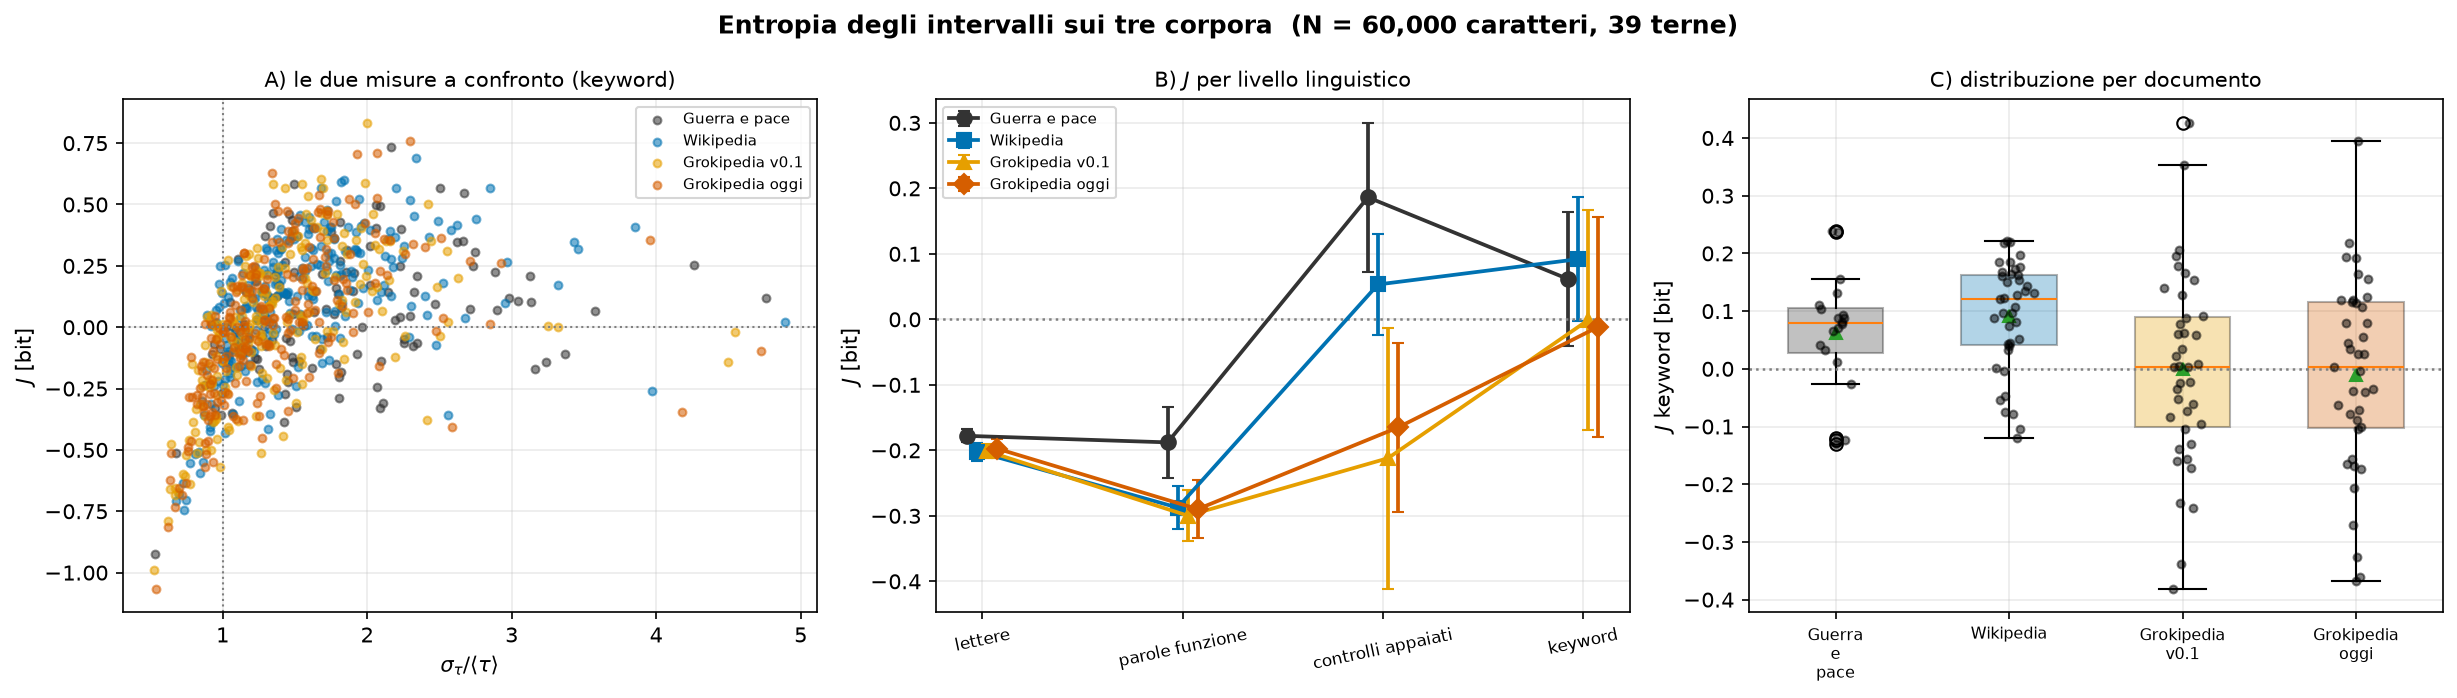
\includegraphics[width=\textwidth]{figure/cap5_entropia_intervalli.png}
  \caption{Entropia degli intervalli. A: relazione fra $J$ e coefficiente di
  variazione sulle parole chiave, un punto per sequenza. B: $J$ ai quattro
  livelli linguistici, con deviazioni standard fra testi; valori negativi
  indicano intervalli più regolari di un processo di Poisson. C: distribuzione
  di $J$ sulle parole chiave documento per documento. La misura è invariante per
  dilatazione dell'asse dei caratteri e non risente quindi della diversa
  lunghezza delle frasi nei due corpora enciclopedici.}
  \label{fig:entropia}
\end{figure}

% ---------------------------------------------------------------------
\section{Quanto pesa la definizione dei livelli lessicali}
\label{sec:effetto-stoplist}

Il paragrafo \emph{Come vengono separati i livelli lessicali} del
§\ref{sec:scelte} ha documentato l'estensione della lista chiusa di parole funzione da
\num{133} a \num{215} voci e la ragione per cui era necessaria. Questa sezione
riporta di quanto si spostano i risultati, perché lo spostamento non è
trascurabile e la scelta deve restare verificabile.

Il pannello A della Figura~\ref{fig:effetto-stoplist} riporta quali parole la
lista originaria lasciava passare fra le parole chiave di Grokipedia, e in
quante voci ciascuna: nell'elenco corrispondente di Wikipedia non ne compare
nessuna, e le sue sette parole sono distinte fra loro, ciascuna in una sola
voce.

\begin{table}[htbp]
  \centering
  \begin{tabular}{lcccc}
    \toprule
    & \multicolumn{2}{c}{lista originaria} & \multicolumn{2}{c}{lista estesa} \\
    \cmidrule(lr){2-3}\cmidrule(lr){4-5}
    & Wikipedia & Grok. oggi & Wikipedia & Grok. oggi \\
    \midrule
    keyword più bursty del controllo & $0.685$ & $0.630$ & $0.692$ & $0.740$ \\
    idem, su $\hat\gamma$ & $0.736$ & $0.663$ & $0.747$ & $0.791$ \\
    $\sigma_\tau/\langle\tau\rangle$ keyword & $1.530$ & $1.289$ & $1.536$ & $1.379$ \\
    divario appaiato, keyword & \multicolumn{2}{c}{$-0.230$} & \multicolumn{2}{c}{$-0.167$} \\
    divario appaiato, controlli & \multicolumn{2}{c}{$-0.122$} & \multicolumn{2}{c}{$-0.157$} \\
    $J$ keyword & $+0.086$ & $-0.069$ & $+0.092$ & $-0.011$ \\
    $\mu$ keyword & $2.38$ & $2.52$ & $2.37$ & $2.19$ \\
    quadrante basso-sinistra & $5.1\%$ & $24.5\%$ & $5.1\%$ & $14.3\%$ \\
    \bottomrule
  \end{tabular}
  \caption{Effetto della definizione dei livelli lessicali sui risultati del
  capitolo. Le righe dei divari appaiati riportano un solo valore perché
  misurano la differenza fra i due corpora. Le lettere e le parole funzione non
  compaiono perché nessuna parola cambia livello a quelle altezze: i loro valori
  coincidono a tutte le cifre riportate nel capitolo.}
  \label{tab:effetto-stoplist}
\end{table}

La Tabella~\ref{tab:effetto-stoplist} riporta il confronto. Tre risultati
cambiano in modo sostanziale. Il primo è il test interno: con la lista
originaria Grokipedia sembrava battere il proprio controllo appaiato meno spesso
di Wikipedia, e l'ordinamento fra i corpora appariva netto; con la lista estesa
l'ordine si inverte, e la differenza fra le due enciclopedie sparisce. Il
pannello B della figura mostra i due esiti sovrapposti. Il secondo è l'entropia
degli intervalli, il cui valore sulle parole chiave passa da $-0.069$ a
$-0.011$, cioè da un cambio di segno netto a uno indistinguibile da zero. Il
terzo è l'esponente di coda, che su Grokipedia scende da $2.52$ a $2.19$,
avvicinandosi a quello di Wikipedia anziché allontanarsene.

Restano invece stabili il divario appaiato complessivo, che si riduce da
$-0.230$ a $-0.167$ senza perdere significatività, il coefficiente di variazione
delle parole chiave, e l'intera decomposizione della~\eqref{eq:eq4}. Non si
muovono di una cifra, come è ovvio, i livelli delle lettere e delle parole
funzione.

La lezione metodologica vale al di là di questo caso. La distinzione fra
parole di contenuto e parole di servizio è la premessa dell'intero protocollo
di~\cite{altmann2012}, e viene qui operata da una lista chiusa che il paper
non specifica. Quando i corpora confrontati hanno abitudini lessicali diverse,
e un modello linguistico ne ha rispetto a un redattore umano, una lista
incompleta non introduce un rumore simmetrico: sposta sistematicamente in un
solo corpus il confine fra i due livelli, e produce un divario che non c'è.

\begin{figure}[htbp]
  \centering
  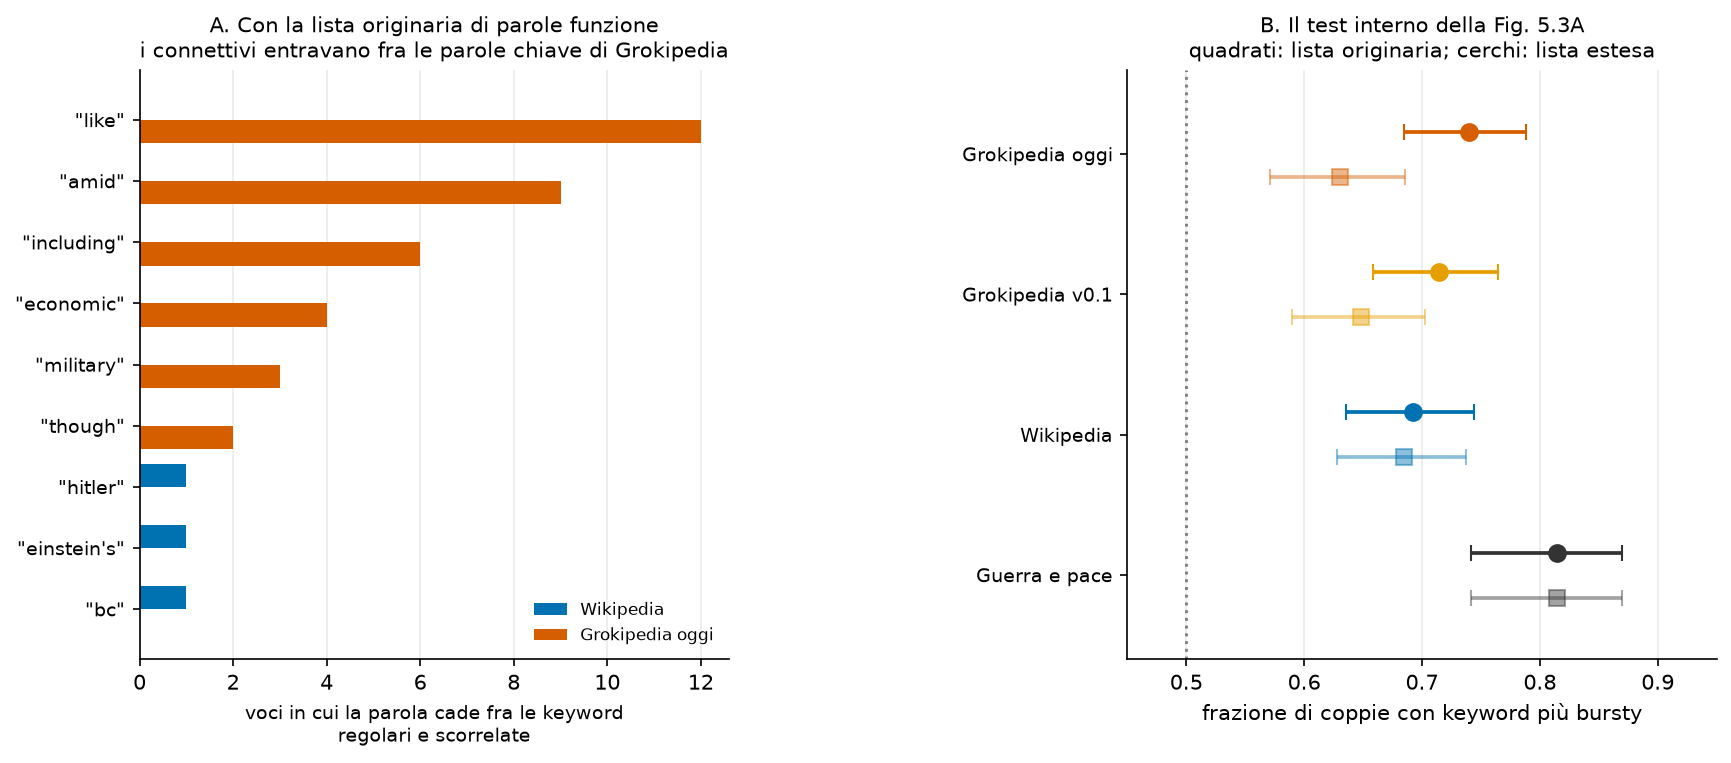
\includegraphics[width=\textwidth]{figure/cap5_effetto_stoplist.png}
  \caption{Effetto della definizione dei livelli lessicali. A: con la lista di
  funtori originaria, quali parole cadevano fra le parole chiave classificate
  come regolari e scorrelate, contate come numero di voci in cui ciò accadeva;
  le prime tre di Grokipedia sono connettivi, e in Wikipedia non compaiono. B:
  il test interno della Figura~\ref{fig:tre-corpora}A con le due
  classificazioni, quadrati per la lista originaria e cerchi per quella estesa,
  con intervalli di confidenza al $95\%$.}
  \label{fig:effetto-stoplist}
\end{figure}

% ---------------------------------------------------------------------
\section{Che cosa il testo generato non riproduce}
\label{sec:sintesi-cap5}

Il testo generato possiede correlazioni a lungo raggio, e ai livelli bassi della
gerarchia linguistica le possiede quasi nella stessa misura del testo umano:
sulle lettere i quattro corpora sono indistinguibili per coefficiente di
variazione, per entropia degli intervalli e per quota di burstiness, e sulle
parole funzione la differenza è piccola, benché significativa. Al livello delle parole il divario si apre, e vale più di un ordine
di grandezza rispetto a quello misurato sui caratteri.

Il divario non distingue però le parole che portano il contenuto dai controlli a
frequenza appaiata. I due valori sono quasi uguali alla lunghezza di lavoro,
$-0.157$ e $-0.167$, e si invertono a quella di controllo
(§\ref{sec:robustezza-neff}); e il test che chiede se la parola chiave superi il
proprio controllo \emph{dentro lo stesso testo} dà a Grokipedia un esito pari a
quello di Wikipedia, anzi lievemente migliore. Il meccanismo descritto
in~\cite{altmann2012} è dunque presente nel testo generato, e con la stessa
efficacia: ciò che manca è l'ampiezza con cui le parole, di contenuto e non, si
addensano.

Non si tratta dunque di una persistenza tematica assente, perché la distinzione
fra parole tematiche e parole ordinarie il modello la produce; si tratta di una
compressione uniforme della variabilità lessicale, che riduce la burstiness di
tutte le parole senza alterare il rapporto fra le une e le altre. Vale ancora la
distinzione posta nel §\ref{sec:intro-linguaggio} fra riprodurre le proprietà
statistiche del linguaggio e riprodurre il meccanismo che le genera, ma
applicata a un livello più basso di quanto la prima lettura suggerisse.

Ciò che il capitolo misura è la distanza fra due enciclopedie appaiate titolo
per titolo, e null'altro. Il deficit è osservato su Grokipedia, cioè su un unico
sistema generativo, in un unico dominio e in una sola lingua: nulla di quanto
riportato qui stabilisce che sia una proprietà dei modelli linguistici in
generale anziché di quel sistema. Il Capitolo~\ref{cap:risultati1} non offre un
appoggio indipendente su questo punto: misura un altro corpus, con grandezze
che non arrivano al livello a cui il divario si manifesta.

%
%  Tre lunghezze di analisi con corpora diversi, da non confondere:
%    fattibilità  50 000 caratteri, 40 voci  (§5.2)
%    analisi      60 000 caratteri, 39 terne (§5.3--5.7)
%    robustezza   80 000 caratteri, 35 terne (§5.8)
% =====================================================================

\chapter{Burstiness lessicale in corpora umani e generativi}
\label{cap:risultati2}

% ---------------------------------------------------------------------
\section{Perché un secondo corpus}
\label{sec:perche-wiki}

Questo capitolo nasce da un esito negativo del precedente. Il
§\ref{sec:fallimenti} ha mostrato che dei \num{242} documenti generati lungo lo
sweep soltanto due non ricadono in alcuna modalità di degenerazione, ed entrambi
si trovano a $T = 1.0$. Il protocollo introdotto nel §\ref{sec:burst} è però un
protocollo semantico: richiede di individuare in ciascun testo le parole che ne
portano il contenuto e di misurare come si distribuiscono le distanze fra le
loro occorrenze successive. Su un testo che ripete lo stesso ciclo di parole, o
su una sequenza degenerata nel senso opposto, 
quelle distanze si calcolano ancora ma non misurano più la
persistenza di un tema. Applicare il protocollo al corpus dello sweep
restituirebbe numeri privi di contenuto.

Il confronto viene quindi spostato su un dominio in cui la qualità del testo
non è una variabile. Wikipedia e Grokipedia trattano le stesse voci, la prima
scritta da esseri umani e la seconda generata da un modello linguistico, ed
entrambe producono prosa espositiva ben formata. Appaiare le due enciclopedie
per titolo tiene inoltre fisso l'argomento trattato: la voce
\emph{Albert Einstein} di Wikipedia e quella di Grokipedia parlano della stessa
cosa, e qualunque differenza nella statistica degli intervalli non può essere
attribuita a un argomento diverso. I corpora sono descritti nel §\ref{sec:corpora}, e le
due versioni di Grokipedia nel §\ref{sec:paternita}.

Il romanzo di riferimento resta nell'analisi come ancora letteraria: è il
dominio su cui il protocollo è stato formulato, e serve a dire quanto la prosa
enciclopedica si discosti già di per sé dal caso studiato in origine.

% ---------------------------------------------------------------------
\section{Il protocollo regge sulla prosa enciclopedica}
\label{sec:fattibilita}

Prima di confrontare due enciclopedie occorre stabilire che l'effetto da
confrontare esista nella prima. Il protocollo di Altmann è stato costruito e
validato su romanzi, e la prosa enciclopedica ha una struttura diversa: non ha
trama, procede per sezioni tematiche dichiarate da titoli, e la persistenza di
un argomento vi si manifesta in modo più rigido. Che le parole di contenuto vi
risultino più \emph{bursty} dei propri controlli non è quindi scontato.

La verifica è stata condotta su \num{40} voci di Wikipedia troncate a
\num{50000} caratteri, contro \num{20} segmenti del romanzo della stessa
lunghezza: è la fase di fattibilità della Tabella~\ref{tab:fasi}, l'unica del
capitolo a impiegare quella lunghezza e quel numero di voci, e i suoi
denominatori non vanno confusi con quelli delle sezioni successive. La
Figura~\ref{fig:wiki-fattibilita} ne riporta l'esito. Il primo
pannello confronta ciascuna parola chiave con il proprio controllo appaiato in
frequenza e riporta la quota di confronti vinti dalla parola chiave: il valore
$0.5$ corrisponde all'assenza di effetto. Su Wikipedia la quota vale
$197/280 = 0.704$ per il coefficiente di variazione e $216/280 = 0.771$ per
l'esponente di correlazione, con estremi inferiori degli intervalli di
confidenza pari a $0.65$ e $0.72$: l'effetto esiste. Sul romanzo le stesse
quote valgono $104/140 = 0.743$ e $123/140 = 0.879$, cioè sono più alte, ma la
differenza non annulla il segnale enciclopedico.

Il secondo pannello mostra da dove viene quel segnale, ed è utile precisare
come i suoi valori siano costruiti, perché la stessa procedura vale per tutte
le figure per livello del capitolo. Dentro ciascun testo si selezionano più
sequenze per livello: diciannove lettere, sei parole funzione, sette parole
chiave e i sette controlli appaiati. Per ognuna si misura
$\sigma_\tau/\langle\tau\rangle$ sui suoi intervalli. I valori delle sequenze
dello stesso livello si mediano poi dentro il testo, ottenendo un
numero per coppia (testo, livello); infine si media su tutti i testi del
corpus, ed è questo secondo valore a comparire nel pannello, con la barra
d'errore data dalla deviazione standard fra testi. Con questa costruzione il
coefficiente di variazione $CV$ cresce salendo lungo i quattro livelli in entrambi
i corpora e con lo stesso andamento: le lettere stanno sotto l'unità, cioè si
distribuiscono in modo più regolare di un processo di Poisson, mentre le
parole chiave arrivano a $1.51$ su Wikipedia e a $1.62$ sul romanzo. Il terzo
pannello riporta la distribuzione dei singoli testi attorno a quelle medie e
mostra che la sovrapposizione fra i due corpora è ampia, con mediane vicine e
code che si intersecano.

Il rapporto fra le due burstiness delle parole chiave vale $0.93$: la prosa
enciclopedica è meno \emph{bursty} del romanzo, ma dello stesso ordine. Il protocollo
regge, e il confronto con Grokipedia ha un segnale da rilevare.

\begin{figure}[htbp]
  \centering
  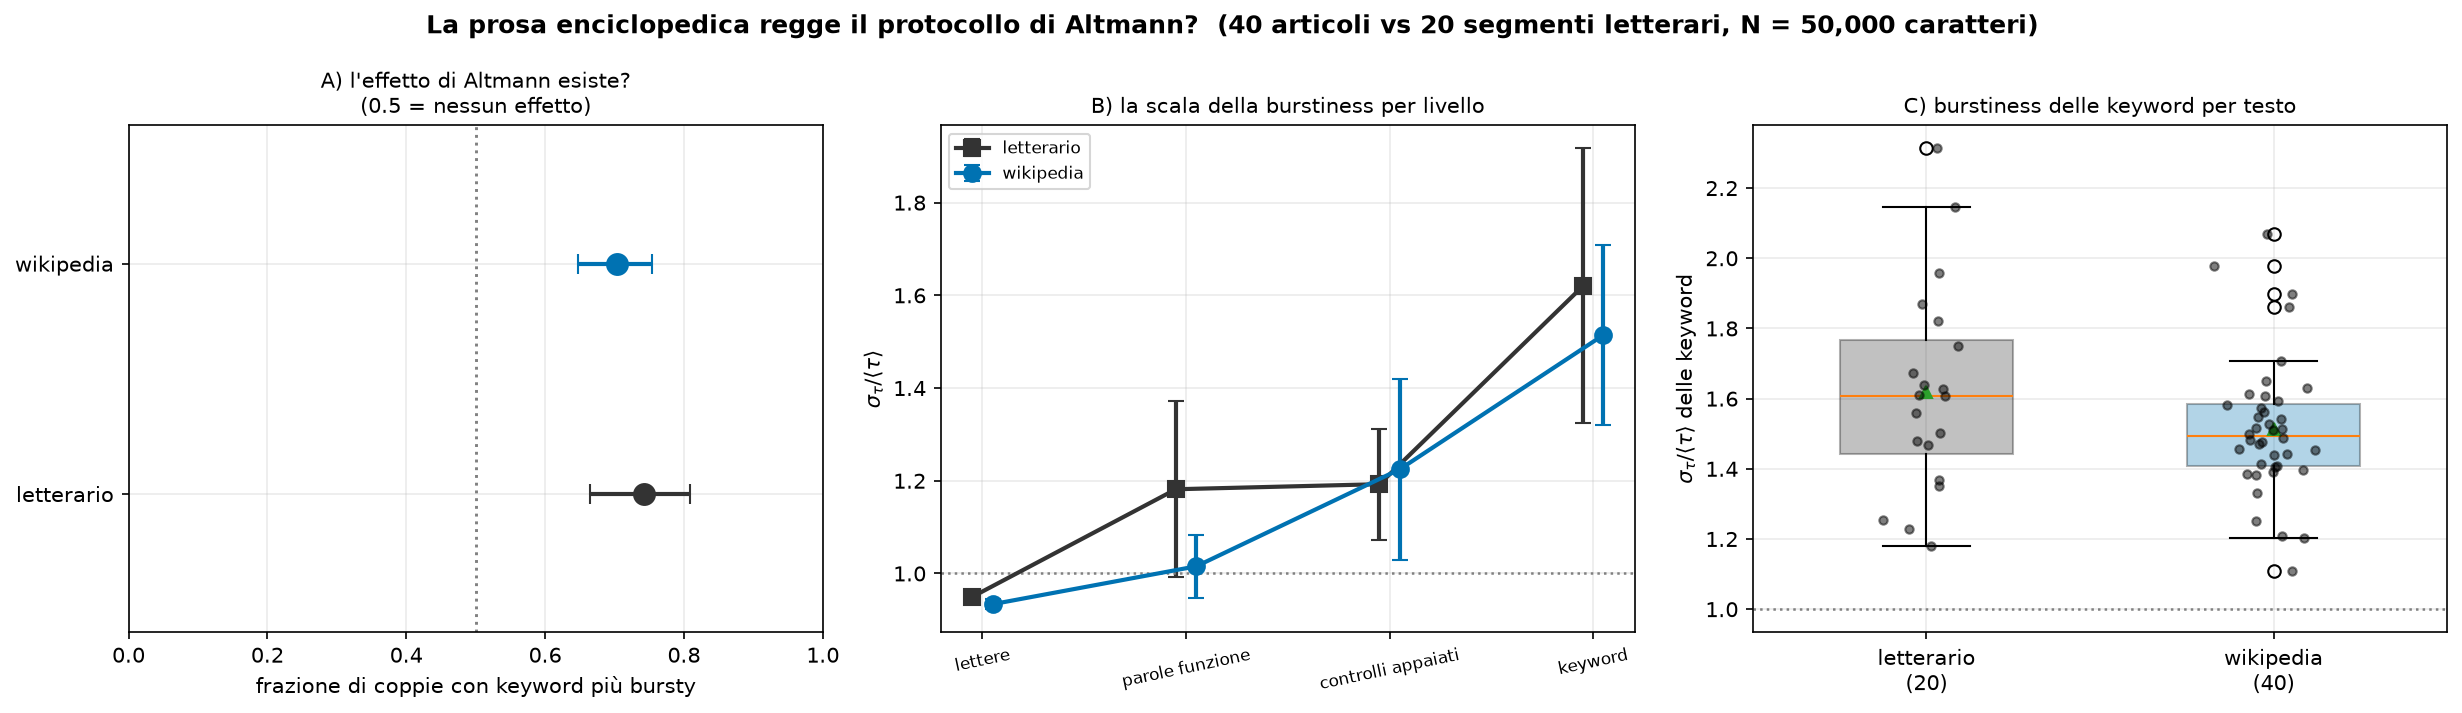
\includegraphics[width=\textwidth]{figure/cap5_wiki_altmann.png}
  \caption{Test di fattibilità del protocollo su prosa enciclopedica, condotto
  su \num{40} voci di Wikipedia e \num{20} segmenti letterari a \num{50000}
  caratteri. A: quota di confronti in cui la parola chiave supera il proprio
  controllo appaiato in frequenza, con intervallo di confidenza al $95\%$; la
  linea punteggiata a $0.5$ è l'assenza di effetto. B: coefficiente di
  variazione degli intervalli ai quattro livelli linguistici. C: distribuzione
  della burstiness delle parole chiave testo per testo. Questa è l'unica figura
  del capitolo costruita su \num{40} voci e \num{50000} caratteri; tutte le
  successive usano \num{39} terne e \num{60000} caratteri.}
  \label{fig:wiki-fattibilita}
\end{figure}

% ---------------------------------------------------------------------
\section{L'effetto nei tre corpora}
\label{sec:tre-corpora}

L'analisi principale confronta Wikipedia, le due versioni di Grokipedia e
l'ancora letteraria su \num{39} terne complete, troncate a \num{60000}
caratteri. La voce esclusa è \emph{Buddhism}, per la ragione riportata nel
§\ref{sec:paternita}: la sua versione v0.1 è ricopiata da Wikipedia, e in un
disegno appaiato un titolo che cade in un corpus deve cadere in tutti.

\paragraph{La finestra su cui l'esponente è stimato.}
L'esponente di correlazione $\hat\gamma$ è ottenuto interpolando
la~\eqref{eq:sigma} nell'intervallo fisso $t \in (100, 2000)$ caratteri.
\cite{altmann2012} adotta invece una regola relativa e ferma la finestra
all'uno per cento della lunghezza del testo. Le due scelte non sono ordinabili
una volta per tutte: applicata ai romanzi interi che quel lavoro analizza la
regola relativa dà un tetto dell'ordine di \num{10000} caratteri, molto più
largo di quello adottato qui; applicata alle finestre da \num{60000} caratteri
di questo capitolo dà $t < 600$, molto più stretto. L'intera catena è stata
ripetuta anche con la seconda. Il
livello medio di $\hat\gamma$ si abbassa di qualche centesimo, sulle parole
chiave da $1.23$ a $1.18$ per Wikipedia e da $1.32$ a $1.22$ per il romanzo,
ma l'ordinamento fra i corpora resta identico a tutti e quattro i livelli. Il
divario appaiato fra Grokipedia attuale e Wikipedia sulle parole chiave passa
da $-0.049$ a $-0.076$, cioè si accentua invece di ridursi, e resta
significativo in entrambi i casi. Le conclusioni di questo capitolo non
dipendono dunque dalla finestra scelta.

\paragraph{Tre modi di leggere il confronto.}
La Figura~\ref{fig:tre-corpora} riporta i tre modi in cui il confronto può
essere letto. Il primo pannello ripete il test del paragrafo precedente sui
quattro corpora: la quota di confronti vinti dalle parole chiave vale
$114/140 = 0.814$ sul romanzo, $189/273 = 0.692$ su Wikipedia,
$195/273 = 0.714$ su Grokipedia v0.1 e $202/273 = 0.740$ su Grokipedia nella
versione attuale. Ripetendo lo stesso test sull'esponente di correlazione
$\hat\gamma$ anziché sulla burstiness, la quota di confronti vinti dalle parole
chiave vale $0.907$ sul romanzo, $0.747$ su Wikipedia, $0.769$ su Grokipedia
v0.1 e $0.791$ su Grokipedia nella versione attuale.
L'effetto esiste ovunque, con tutti e quattro gli
intervalli di confidenza interamente sopra $0.5$, ed è massimo sul romanzo;
fra le due enciclopedie, però, non distingue: i valori di Grokipedia sono anzi
lievemente superiori a quelli di Wikipedia, con intervalli che si sovrappongono.
La domanda a cui questo pannello risponde è se la parola chiave superi il
proprio controllo a frequenza appaiata dentro lo stesso testo, e la
risposta è che ciò accade con la stessa frequenza nei due corpora enciclopedici.
Il deficit di Grokipedia, misurato dai pannelli successivi, non riguarda dunque
l'esistenza del meccanismo ma il livello assoluto della burstiness.

Il secondo pannello mostra il coefficiente di variazione ai quattro livelli e
rende visibile dove la differenza si concentra. Sulle lettere i quattro corpora
sono indistinguibili, tutti compresi fra $0.922$ e $0.950$, e sulle parole
funzione la separazione resta modesta, da $0.967$ a $1.192$. Il divario si apre
ai due livelli lessicali: sui controlli appaiati il romanzo raggiunge $1.262$,
Wikipedia $1.190$ e le due versioni di Grokipedia $1.044$ e $1.055$; sulle
parole chiave rispettivamente $1.789$, $1.536$, $1.387$ e $1.379$. 
Il terzo pannello riporta la stessa quantità testo per testo,
e mostra che la separazione non è l'effetto di pochi articoli anomali: le
distribuzioni di Wikipedia e di Grokipedia si sovrappongono, ma le loro mediane
differiscono di circa $0.25$ e la coda superiore di Wikipedia è più popolata.

\begin{figure}[htbp]
  \centering
  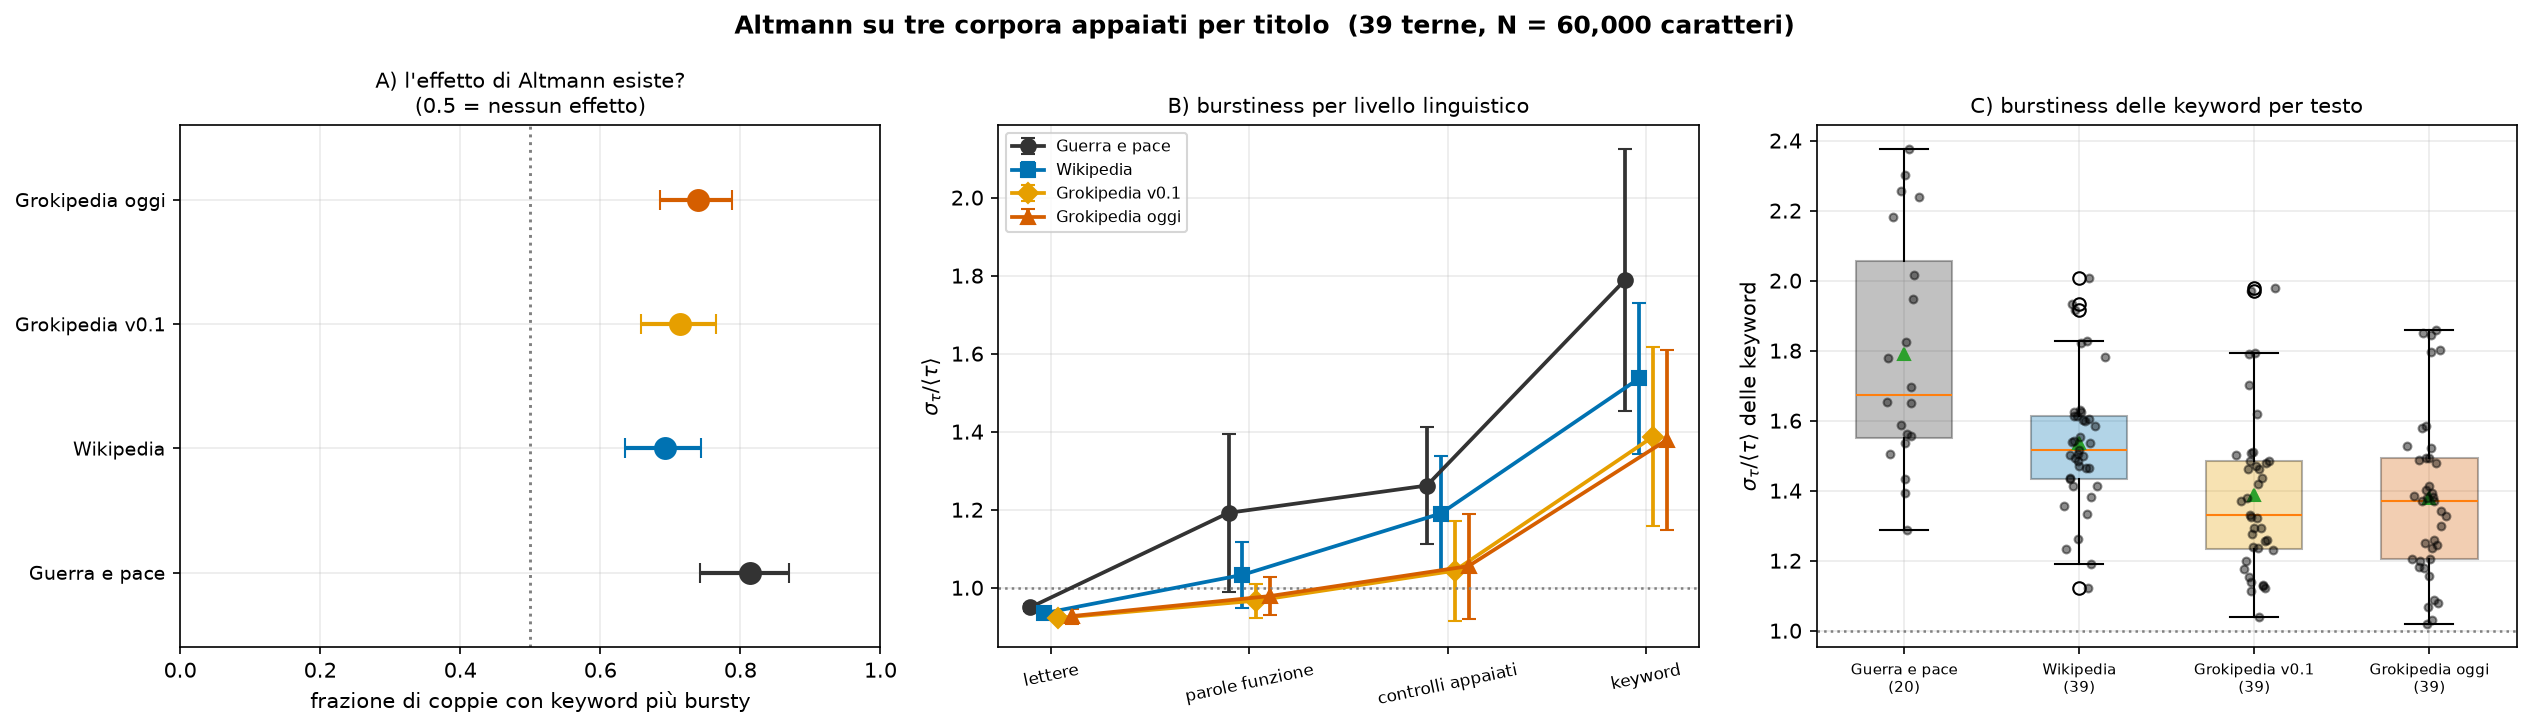
\includegraphics[width=\textwidth]{figure/cap5_tre_corpora.png}
  \caption{Il protocollo di Altmann sui quattro corpora, \num{39} terne
  appaiate per titolo a \num{60000} caratteri. A: quota di confronti vinti dalle
  parole chiave, con intervallo di confidenza al $95\%$. B: coefficiente di
  variazione degli intervalli ai quattro livelli linguistici; le barre sono
  deviazioni standard fra testi. C: burstiness delle parole chiave testo per
  testo, con mediana, quartili e singoli punti sovrapposti. Il numero di testi
  per corpus è indicato sotto ciascuna colonna.}
  \label{fig:tre-corpora}
\end{figure}

\paragraph{L'ancora letteraria è un testo, non un genere.} Il primato del
romanzo sui due livelli lessicali non sopravvive al cambio di testo. Ripetendo
l'intera misura su tre altri romanzi inglesi trattati esattamente come
\emph{Guerra e pace}, cioè \emph{Moby Dick}, \emph{Middlemarch} e \emph{David
Copperfield}, gli stessi impiegati come controllo nel
§\ref{sec:coda-risultati}, sulle parole chiave si ottiene $1.55$, $1.54$ e
$1.63$, cioè valori sostanzialmente pari a quello di Wikipedia e ben al di
sotto dell'$1.79$ di \emph{Guerra e pace}; alle parole funzione si ottiene
$1.03$, $1.08$ e $1.09$, contro l'$1.19$ del romanzo di riferimento e l'$1.03$
di Wikipedia. La distanza fra prosa letteraria e prosa enciclopedica non è
dunque un fatto generale, e l'ancora letteraria di questo capitolo va letta
per ciò che è: un termine di paragone concreto, non la misura di un genere.
Nulla di ciò che segue vi poggia, perché il risultato del capitolo è un
confronto appaiato fra le due enciclopedie, dove il romanzo non entra.

Il null model A1 restituisce un esponente medio di $0.983$ su tutte le celle,
in accordo con l'unità che deve dare per costruzione: la procedura di stima si
comporta come nel §\ref{sec:validazione} anche su questi corpora.

\paragraph{L'analogo della Figura~2 di~\cite{altmann2012}.}
La Figura~\ref{fig:altmann-fig2} riproduce sui quattro corpora la costruzione
con cui~\cite{altmann2012} presenta il proprio risultato principale, e permette
di verificarne l'aderenza riga per riga. Per ogni corpus vengono mostrate una
lettera e una parola di contenuto, ciascuna con la distribuzione cumulata degli
intervalli e con la crescita della varianza del conteggio, accanto alle stesse
curve calcolate sui due null model.

\paragraph{Quale parola mostrare.} La scelta della parola da mostrare pone un
problema che il caso della lettera non ha. Selezionare la parola chiave più
ricorrente del corpus, che è il criterio più immediato, produce oggetti
strutturalmente diversi nei due tipi di prosa: in un romanzo pesca il nome di
un personaggio, presente solo nelle scene in cui il personaggio compare,
mentre in un'enciclopedia pesca il soggetto della voce, che ricorre in quasi
ogni frase. Le due parole finirebbero alle code opposte delle rispettive
distribuzioni di burstiness, al $96$ e al $2$ percentile, e la figura
confronterebbe due casi estremi anziché due casi tipici. La parola mostrata è
quindi quella con $\sigma_\tau/\langle\tau\rangle$ più vicino alla mediana del
proprio corpus, fra quelle con almeno \num{40} occorrenze; il percentile
effettivo è riportato sopra ciascun pannello e sta fra $45$ e $57$ in tutti e
quattro i corpora. Il caso escluso ha però un interesse proprio, ed è ripreso
subito dopo la figura.

\paragraph{Che cosa mostrano le quattro righe.}
Il comportamento è allora quello descritto nel §\ref{sec:origini}, e vale su
tutte e quattro le righe. Sulla lettera la cumulata decade rapidamente e
l'esponente del null model A2 si dispone attorno all'unità, $0.94$ sul romanzo,
$0.90$ su Wikipedia, $0.94$ sulla v0.1 e $1.05$ sulla versione attuale di
Grokipedia, perché a quel livello la burstiness non contribuisce. Lo scarto
massimo da uno vale un decimo, ed è quanto ci si attende su una singola
sequenza: aggregando tutte le \num{2603} sequenze di livello letterale dei
quattro corpora $\hat\gamma_{A2}$ vale fra $0.983$ e $0.990$, con una
dispersione fra sequenze di $0.044$, cosicché i quattro valori della figura
stanno tutti entro due deviazioni standard dall'unità. Un solo caso per corpus
non permette dunque una lettura più fine di così.

Sulla parola di contenuto la cumulata ha coda larga, con
$\sigma_\tau/\langle\tau\rangle$ fra $1.23$ e $1.79$, e $\hat\gamma_{A2}$
resta sopra l'unità e più vicino a $\hat\gamma$ che nel caso della lettera:
$1.36$ contro $1.43$ sul romanzo, $1.09$ contro $1.20$ su Wikipedia, $1.09$
contro $1.23$ sulla v0.1 e $1.11$ contro $1.20$ sulla versione attuale. Una
parte della correlazione passa cioè attraverso la distribuzione degli
intervalli, e la frazione è massima sul romanzo. La figura mostra il
meccanismo su un caso per corpus e non va letta come misura del divario fra
corpora: quella richiede l'aggregato del §\ref{sec:decomposizione}, perché su
una singola parola la differenza fra i due esponenti è dominata dal rumore di
stima. Lo si vede nella riga di Grokipedia attuale, dove sulla lettera
$\hat\gamma = 0.94$ scende sotto $\hat\gamma_{A2} = 1.05$, cosa che
sull'aggregato di quel livello, dove il rumore si media, non accade.

La lettera \emph{e} in \emph{Guerra e pace} dà qui un coefficiente di
variazione pari a $0.85$ contro lo $0.83$ della didascalia della Figura~2
di~\cite{altmann2012}, il che vale come controllo indipendente delle
procedure: la stessa quantità, misurata sullo stesso testo da un codice
diverso, coincide entro due centesimi.

\begin{figure}[htbp]
  \centering
  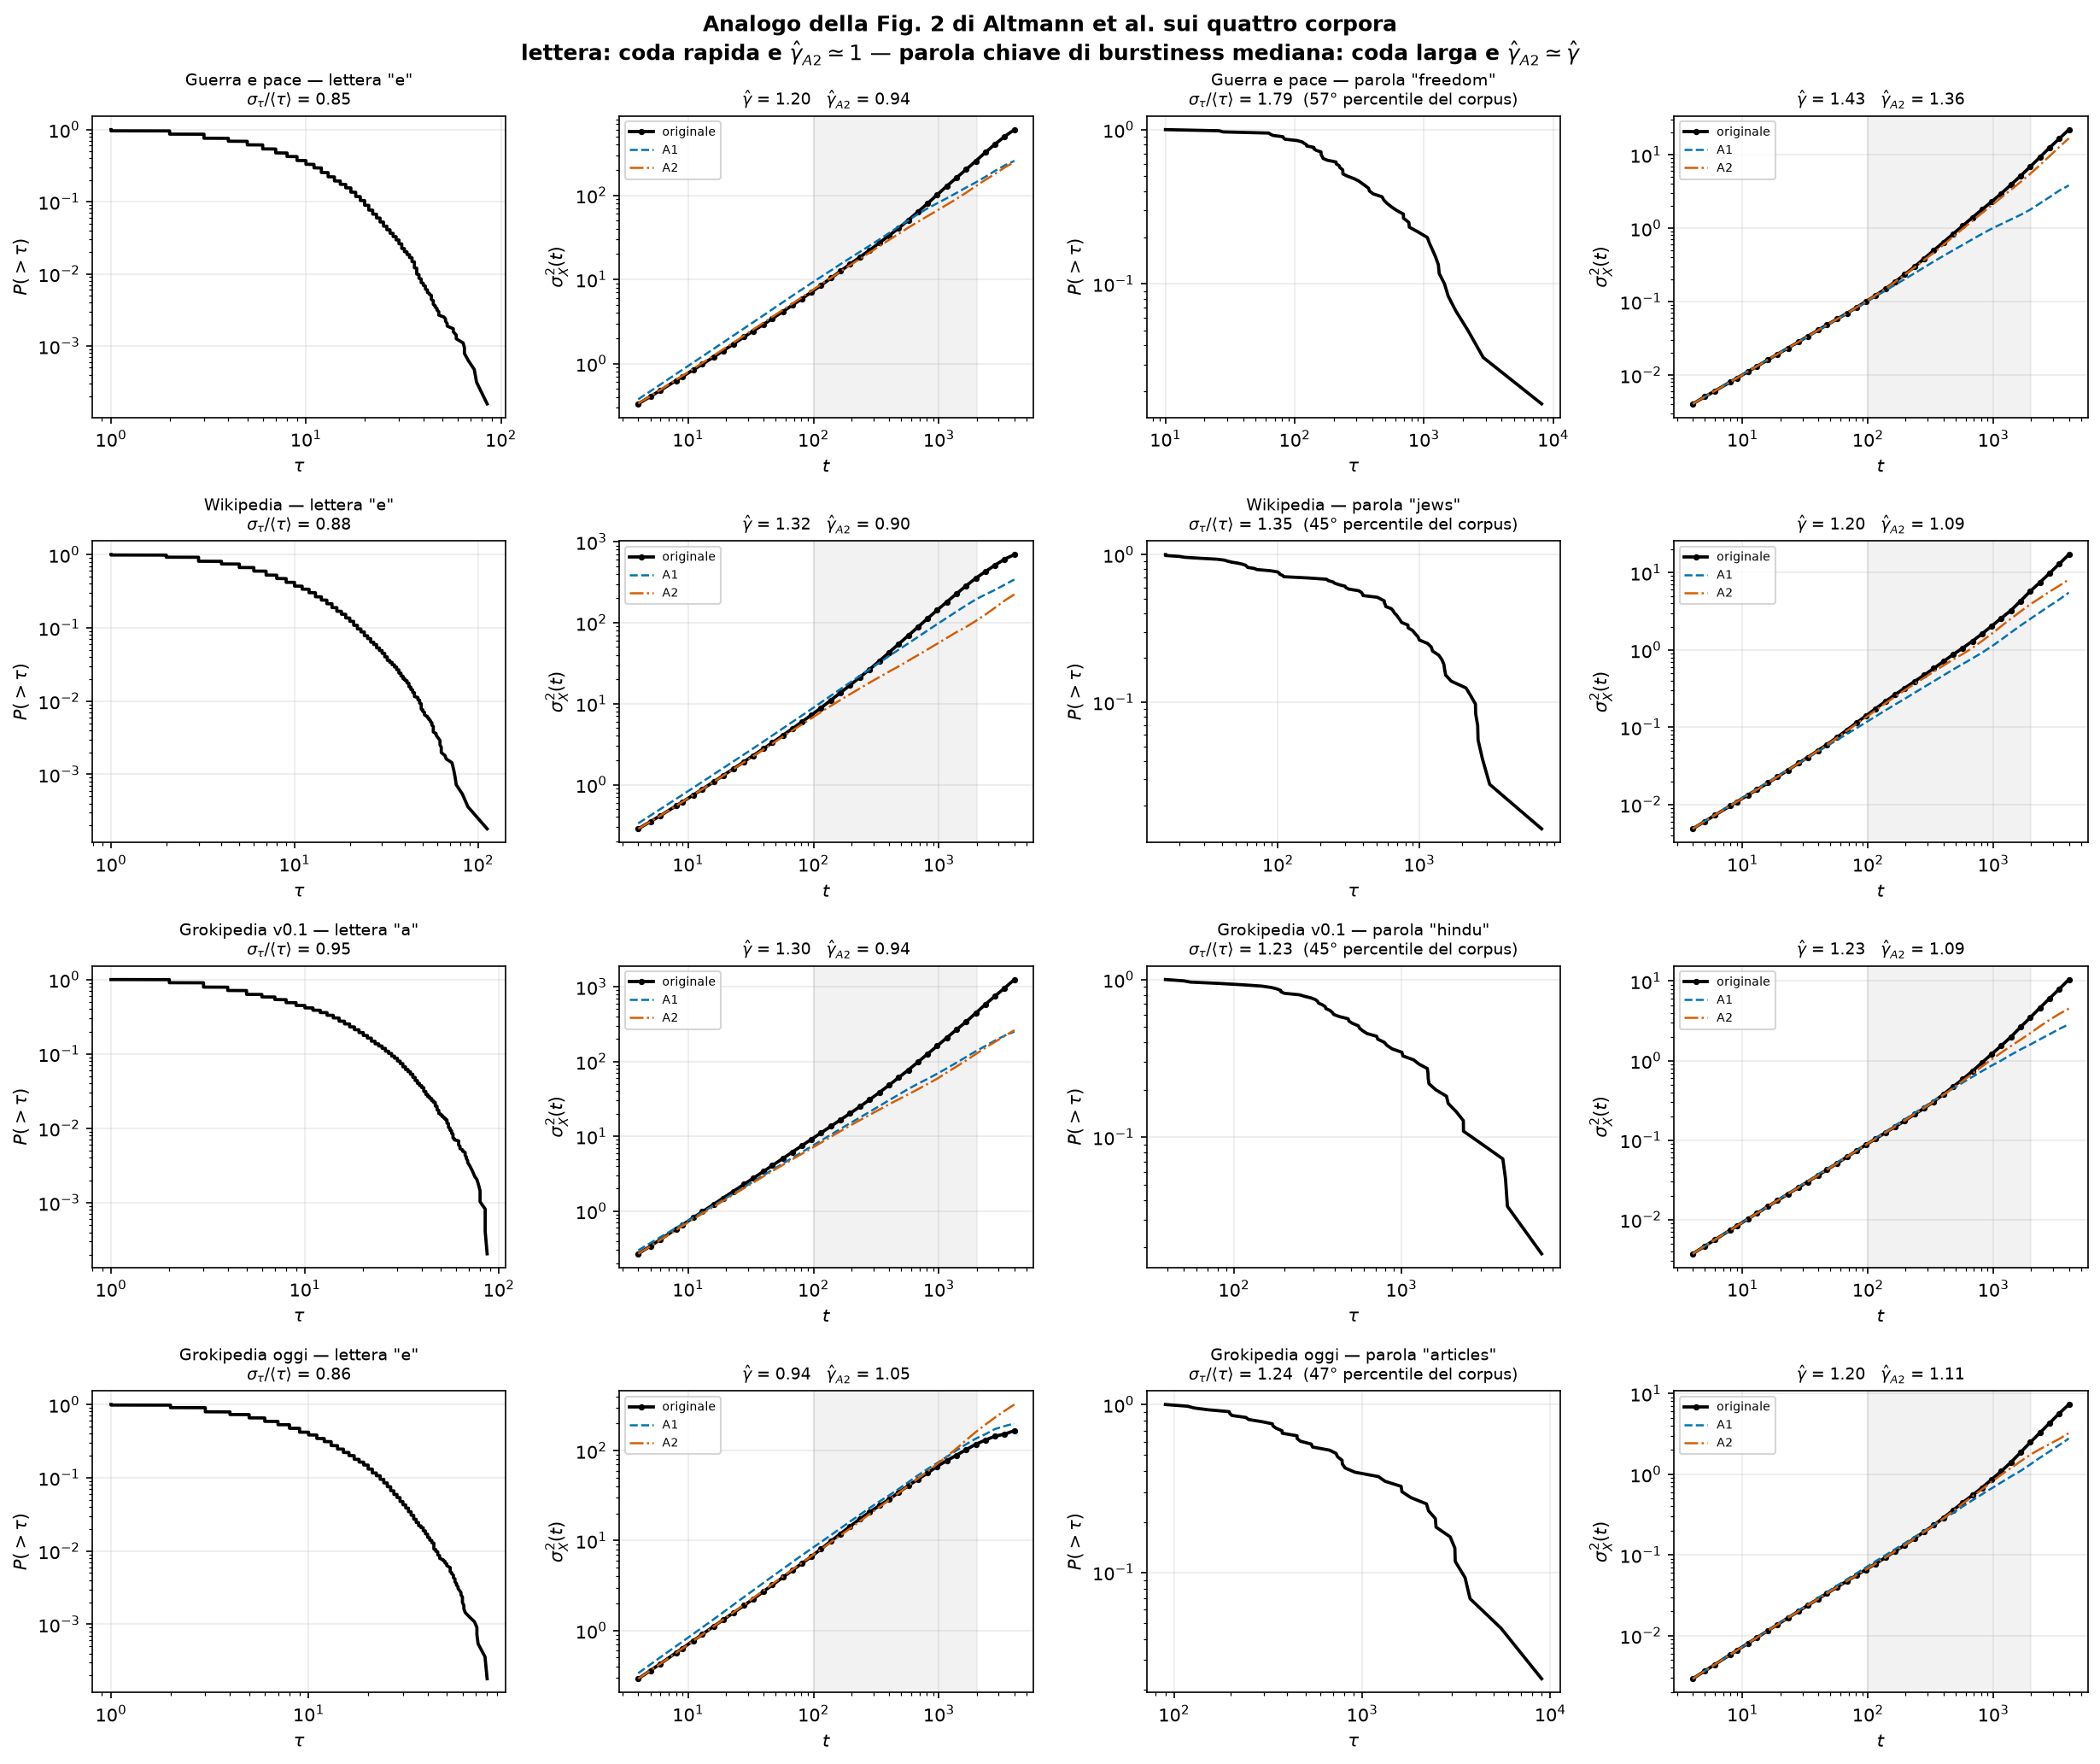
\includegraphics[width=\textwidth]{figure/cap5_altmann_fig2.png}
  \caption{Analogo della Figura~2 di~\cite{altmann2012} sui quattro corpora. Una
  riga per corpus; a sinistra la lettera più frequente del documento, a destra
  la parola chiave di burstiness mediana del corpus fra quelle con almeno
  \num{40} occorrenze, con il suo percentile indicato sopra il pannello. Per
  ciascuna, la distribuzione cumulata degli intervalli $P(>\tau)$ e la crescita
  della varianza del conteggio $\sigma_X^2(t)$, con le curve dei due null model
  del §\ref{sec:null} e la finestra di fit ombreggiata. La lettera ha coda
  rapida e $\hat\gamma_{A2} \simeq 1$; la parola di contenuto ha coda larga e
  $\hat\gamma_{A2}$ prossimo a $\hat\gamma$.}
  \label{fig:altmann-fig2}
\end{figure}

\paragraph{Il soggetto della voce non è una parola di contenuto.}
La parola chiave più ricorrente di un articolo enciclopedico, quella che il
criterio scartato sopra avrebbe selezionato, si comporta in modo opposto a
quello che il §\ref{sec:origini} prevede per il suo livello linguistico. Nella
voce \emph{Alexander the Great} di Wikipedia la parola \emph{alexander} ha
$\sigma_\tau/\langle\tau\rangle = 0.78$; in \emph{Sigmund Freud} di Grokipedia
\emph{freud} ha $0.72$. Sono valori sotto il limite poissoniano, cioè
distribuzioni \emph{più regolari del caso}, mentre la lettera \emph{e} negli
stessi testi dà $0.84$. Il confronto con la lettera non va però fatto sul valore
grezzo. Per un processo casuale in tempo discreto
$\sigma_\tau/\langle\tau\rangle$ non vale esattamente uno, ma tanto meno quanto
più corti sono gli intervalli: il null model A1, applicato alla stessa frequenza
della sequenza osservata, restituisce $0.95$ per la lettera \emph{e}, che ricorre
ogni dieci caratteri, e $1.00$ per una parola chiave, che ricorre ogni
duecento.

\paragraph{Il riferimento casuale dipende dalla frequenza.}
La ragione di quel $0.95$ è che gli intervalli sono numeri interi positivi. Se
le occorrenze sono collocate a caso con probabilità $f$ per carattere, la
distanza fra due consecutive è geometrica, e per la geometrica si ha
$\sigma_\tau/\langle\tau\rangle = \sqrt{1-f}$: il valore tende a uno solo nel
limite di eventi rari. Con $f = 1/10$, la frequenza della lettera \emph{e}, si
ottiene $0.949$; con $f = 1/200$, la frequenza tipica di una parola chiave,
$0.997$. Il valore poissoniano di riferimento non è dunque lo stesso ai due
livelli, ed è più basso proprio dove gli eventi sono più fitti. Confrontare
\emph{alexander} e la lettera \emph{e} sui valori grezzi significherebbe
attribuire alla struttura del testo una differenza che è invece un effetto
della sola frequenza.

Rapportando ciascuna misura al proprio valore casuale l'effetto si toglie, e
resta $0.78$ per \emph{alexander} contro $0.88$ per la lettera: il soggetto
della voce è più regolare di una lettera anche dopo aver tolto l'effetto della
frequenza, e la differenza fra i due, lungi dall'essere prodotta dalla
normalizzazione, ne esce accentuata.

\paragraph{Perché il soggetto si comporta così.}
La ragione è che in prosa enciclopedica il soggetto non è un tema fra altri,
che alterna presenza e assenza lungo il testo, ma il tema unico: compare come soggetto grammaticale di quasi ogni
periodo, e i suoi intervalli ereditano allora la statistica della lunghezza
delle frasi anziché quella dell'alternanza tematica. La verifica è diretta.
Nei sei articoli esaminati il soggetto ricorre una volta ogni $1.4$--$1.7$
frasi, con lo stesso valore in Wikipedia e in Grokipedia. I suoi intervalli sono
quindi lunghezze di frase, e ne ereditano la variabilità: le
lunghezze di frase di quegli articoli hanno
$\sigma_\tau/\langle\tau\rangle$ fra $0.33$ e $0.73$, e il soggetto della voce
si colloca poco sopra, fra $0.54$ e $0.78$, comunque sotto l'unità che
segnerebbe l'assenza di struttura. Per confronto, \emph{natásha} in un segmento
di \emph{Guerra e pace} ricorre una volta ogni $5.1$ frasi e ha
$\sigma_\tau/\langle\tau\rangle = 3.24$: lì la ricorrenza non segue il ritmo del
periodo ma l'alternanza delle scene.

Il soggetto della voce funziona quindi da marcatore sintattico e non semantico,
e la sua ricorrenza è governata dal ritmo del periodo, non dalla persistenza di
un argomento. Non è un difetto della misura ma un tratto del genere
enciclopedico, e va tenuto presente nel confrontare la burstiness lessicale fra
generi diversi: è la ragione per cui la parola mostrata nella
Figura~\ref{fig:altmann-fig2} viene scelta sulla mediana e non sul massimo.

% ---------------------------------------------------------------------
\section{Il divario si apre al livello lessicale}
\label{sec:appaiato}

L'appaiamento per titolo permette un test più stringente del confronto fra
medie. Confrontare la media di Wikipedia con quella di Grokipedia lascia
aperta l'obiezione che le due medie siano calcolate su argomenti diversi, e
che la differenza rifletta il contenuto anziché la scrittura. Il test appaiato
la chiude: per ciascuna delle \num{39} voci, che nei due corpora tratta lo
stesso argomento, si calcola la differenza fra il valore di Grokipedia e
quello di Wikipedia, e si verifica con il test dei ranghi segnati di Wilcoxon
che la mediana di quelle \num{39} differenze sia diversa da zero. Il test è
non parametrico, quindi non assume che le differenze siano distribuite
normalmente, assunzione che con \num{39} osservazioni e distribuzioni
asimmetriche non sarebbe difendibile.

Il test dà, per la versione attuale di Grokipedia,
$-0.167$ sulle parole chiave e $-0.010$ sulle lettere; ai due livelli intermedi
le differenze valgono $-0.037$ per le parole funzione e $-0.157$ per i controlli
appaiati, tutte con significatività inferiore a $10^{-2}$. La versione v0.1 dà
$-0.012$, $-0.039$, $-0.116$ e $-0.133$.

I quattro numeri vanno letti come una scala. Alle lettere Grokipedia e
Wikipedia distano un centesimo di unità di burstiness, cioè circa l'uno per
cento del valore misurato: a quel livello i due corpora sono, in pratica, lo
stesso testo. Alle parole funzione la distanza quadruplica, ma resta piccola in
termini relativi. Ai due livelli lessicali passa a circa sedici centesimi, oltre
un decimo del valore misurato e più di un ordine di grandezza sopra il livello
delle lettere.

La scala ha però un solo gradino, non tre. La differenza fra i livelli
sub-lessicali e quelli lessicali è netta; quella fra i due livelli lessicali non
esiste: $-0.157$ sui controlli a frequenza appaiata contro $-0.167$ sulle parole
chiave sono lo stesso numero. Il testo generato non perde dunque le parole di
contenuto più di quanto perda le altre parole della stessa frequenza. Ciò che i
dati sostengono è che riproduca le regolarità dei livelli bassi e abbassi
uniformemente la burstiness a livello di parola, non che perda selettivamente la
persistenza tematica.

\paragraph{Il divario alla lunghezza di controllo.}
\label{sec:robustezza-neff}
L'intera catena è stata ripetuta a $N_{\mathrm{eff}} = \num{80000}$ caratteri,
lunghezza a cui sopravvivono \num{35} delle \num{39} terne; per isolare
l'effetto della finestra, i valori a \num{60000} sono ricalcolati sulle stesse
\num{35}. Alle lettere e alle parole funzione il divario appaiato è stabile, da
$-0.010$ a $-0.011$ e da $-0.037$ a $-0.045$; ai due livelli lessicali si separa
in direzioni opposte, con i controlli appaiati da $-0.164$ a $-0.195$ e le parole
chiave da $-0.167$ a $-0.130$, quest'ultima con significatività che scende a
$p = 0.027$. Alla lunghezza maggiore il divario sulle parole chiave è dunque
\emph{minore} di quello sui controlli appaiati. Ciò che risulta robusto è il
salto dal livello sub-lessicale a quello lessicale; l'ulteriore crescita fino
alle parole chiave non lo è. Anche l'esponente di coda è instabile fra le due
lunghezze, da $2.19$ a $2.50$ su Grokipedia e da $2.37$ a $2.25$ su Wikipedia,
coerentemente con l'avvertenza del §\ref{sec:coda-risultati}.

La Figura~\ref{fig:altmann-fig3} riporta le stesse sequenze nel piano che
\cite{altmann2012} usa per la propria Figura~3: la burstiness in ascissa e
l'esponente di correlazione in ordinata, un punto per sequenza, con un simbolo
diverso per livello linguistico. La gerarchia vi si legge come una disposizione
spaziale: le lettere, gli spazi e le vocali si addensano in una colonna stretta
attorno a $\sigma_\tau/\langle\tau\rangle \simeq 0.5$, le parole funzione e i
controlli appaiati occupano la regione centrale, le parole chiave si spingono a
destra e in alto. È la stessa gerarchia dei paragrafi precedenti, vista tutta
insieme invece che un livello alla volta.

Il piano rende però visibile anche una proprietà che i confronti per livello
non mostrano, e che è l'osservazione centrale di quel lavoro: l'angolo in
basso a destra è vuoto. Non esistono, cioè, sequenze molto \emph{bursty} e
insieme poco correlate. Sui quattro corpora di questa tesi la regolarità si
quantifica così: delle $451$ sequenze con $\sigma_\tau/\langle\tau\rangle >
1.5$, soltanto $17$, il $3.8\%$, hanno $\hat\gamma < 1.1$, e fra quelle con
burstiness superiore a $2$ l'esponente non scende mai sotto $1.05$. L'angolo
opposto, invece, è popolato: delle $3500$ sequenze sotto il valore poissoniano
$\sigma_\tau/\langle\tau\rangle = 1$, il $15.9\%$ ha $\hat\gamma > 1.2$.

L'asimmetria fra i due angoli è la firma di una relazione a senso unico. La
burstiness produce correlazione, come mostra la~\eqref{eq:eq4}, e una sequenza
con vuoti lunghi non può quindi risultare scorrelata; il viceversa non vale,
perché la correlazione può venire anche dall'ordine degli intervalli e
manifestarsi senza alcuna coda pesante. La correlazione di rango fra le due
quantità è positiva e significativa in tutti e quattro i corpora, da $+0.22$ su
Wikipedia a $+0.36$ sul romanzo. Il meccanismo descritto in~\cite{altmann2012}
sui romanzi si ritrova dunque identico nella prosa enciclopedica e in quella
generata, ed è un risultato indipendente dal divario misurato sopra: riguarda
come le due grandezze si legano fra loro, non quanto valgano.

\begin{figure}[htbp]
  \centering
  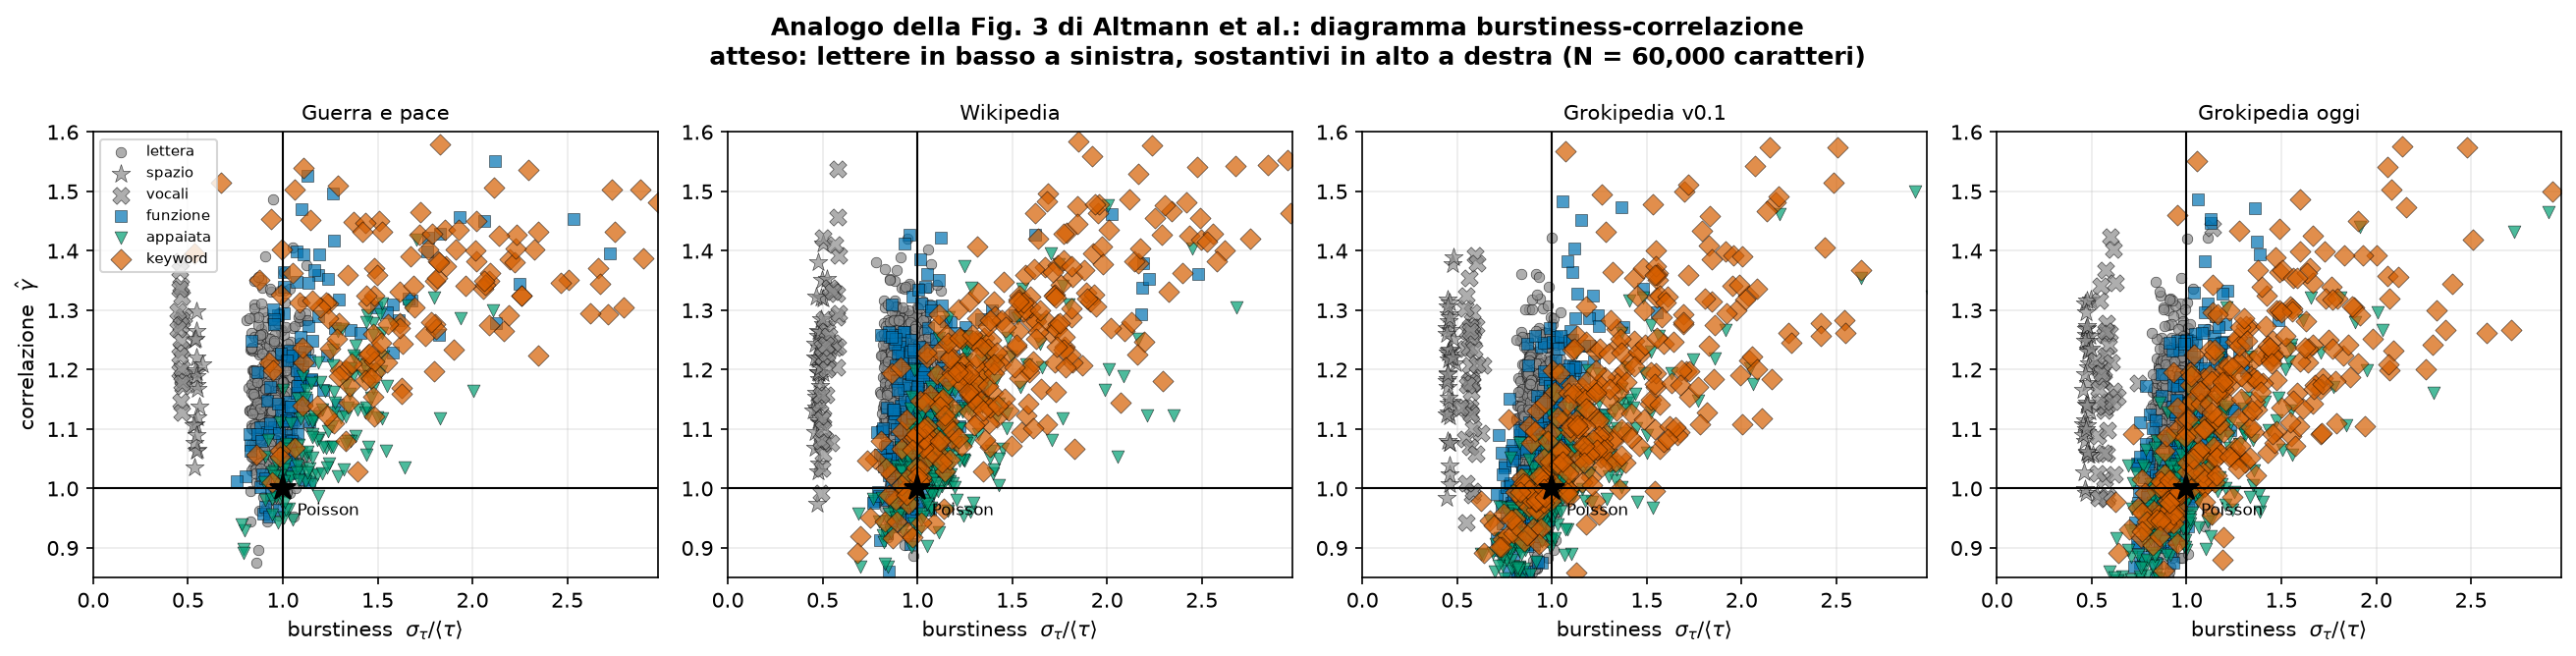
\includegraphics[width=\textwidth]{figure/cap5_altmann_fig3.png}
  \caption{Analogo della Figura~3 di~\cite{altmann2012}: diagramma
  burstiness--correlazione sui quattro corpora, un punto per sequenza. Oltre ai
  quattro livelli usati nel resto del capitolo sono riportati i due livelli
  sub-lessicali tenuti come diagnostica, gli spazi e le vocali. Le linee nere
  segnano il processo di Poisson,
  $\sigma_\tau/\langle\tau\rangle = 1$ e $\hat\gamma = 1$. L'angolo in basso a
  destra è praticamente vuoto in tutti e quattro i corpora: sequenze molto
  bursty e insieme poco correlate non si osservano.}
  \label{fig:altmann-fig3}
\end{figure}

\paragraph{I due quadranti che restano.} La lettura del piano fatta finora
riguarda la diagonale: l'angolo in basso a destra vuoto e quello in alto a
sinistra popolato. Gli altri due separano però i corpora meglio di qualunque
media, e la Figura~\ref{fig:quadranti} li riporta separatamente. Fra le parole
chiave, l'angolo in alto a destra è la posizione canonica
di~\cite{altmann2012}, quella in cui la sequenza è insieme bursty e correlata.
Vi ricade il $91.4\%$ delle sequenze di \emph{Guerra e pace} e l'$87.5\%$ di
quelle di Wikipedia, ma solo il $74.0\%$ di Grokipedia v0.1 e il $77.3\%$
della versione attuale. La differenza finisce quasi interamente nell'angolo
opposto, in basso a sinistra, dove la parola è più regolare di un processo di
Poisson e insieme priva di correlazione a lungo raggio: $0\%$ sul romanzo,
$5.1\%$ su Wikipedia, $15.4\%$ su Grokipedia v0.1 e $14.3\%$ sulla versione
attuale. Una parola chiave generata su sette si trova dunque nell'angolo
opposto a quello canonico, contro una su venti in Wikipedia. Il test appaiato
sulle \num{39} voci conferma che non è un effetto di composizione del
campione: la quota di parole chiave in basso a sinistra cresce in $21$ e $22$
voci su $39$, con differenza mediana $+0.143$ e $p < 10^{-3}$ per entrambe le
versioni.

Due controlli escludono le spiegazioni strumentali. Il null model A1
restituisce $\hat\gamma = 0.983$ in tutti e quattro i corpora, identico alla
terza cifra, quindi la soglia $\hat\gamma = 1$ non è tarata diversamente da un
corpus all'altro; il valore calibrato non è però esattamente uno, cosicché la
soglia è lievemente generosa verso il lato correlato, allo stesso modo per
tutti. E la quota di parole in basso a sinistra resta più alta in Grokipedia
dentro quattro fasce di frequenza su cinque, da $0.159$ contro $0.050$ per le
parole con $26$--$35$ occorrenze a $0.303$ contro $0.076$ per quelle con più di
$80$. Fa eccezione la fascia più bassa, $15$--$25$ occorrenze, dove il rapporto
si inverte, $0.065$ contro $0.200$; lì però le parole chiave di Wikipedia sono
dieci in tutto e la quota è stimata su di esse. Il divario non dipende quindi
dal fatto che le parole chiave di Wikipedia siano più frequenti, salvo nella
fascia in cui il confronto ha meno appoggio.

Guardare dentro il quadrante non rivela più un gruppo omogeneo. Separando le
parole che compaiono nel titolo della voce dalle altre, le $14$ di Wikipedia si
dividono a metà, e le $39$ di Grokipedia si dividono in $18$ soggetti di voce e
$21$ altre parole, prevalentemente aggettivi generici: \emph{economic} in cinque
voci, \emph{military} in tre, \emph{urban} in due. Sono concentrazioni modeste,
e soprattutto non sono più quelle che la lista di parole funzione originaria
lasciava passare: con quella lista, il quadrante conteneva \emph{like} in dodici
voci, \emph{amid} in nove e \emph{including} in sei, cioè i connettivi che
costituiscono il vizio stilistico più evidente del testo generato. Quei termini
sono ora classificati come parole funzione, che è ciò che sono, e il
§\ref{sec:effetto-stoplist} misura quanto la loro presenza fra le parole chiave
alterasse i risultati.

\begin{figure}[htbp]
  \centering
  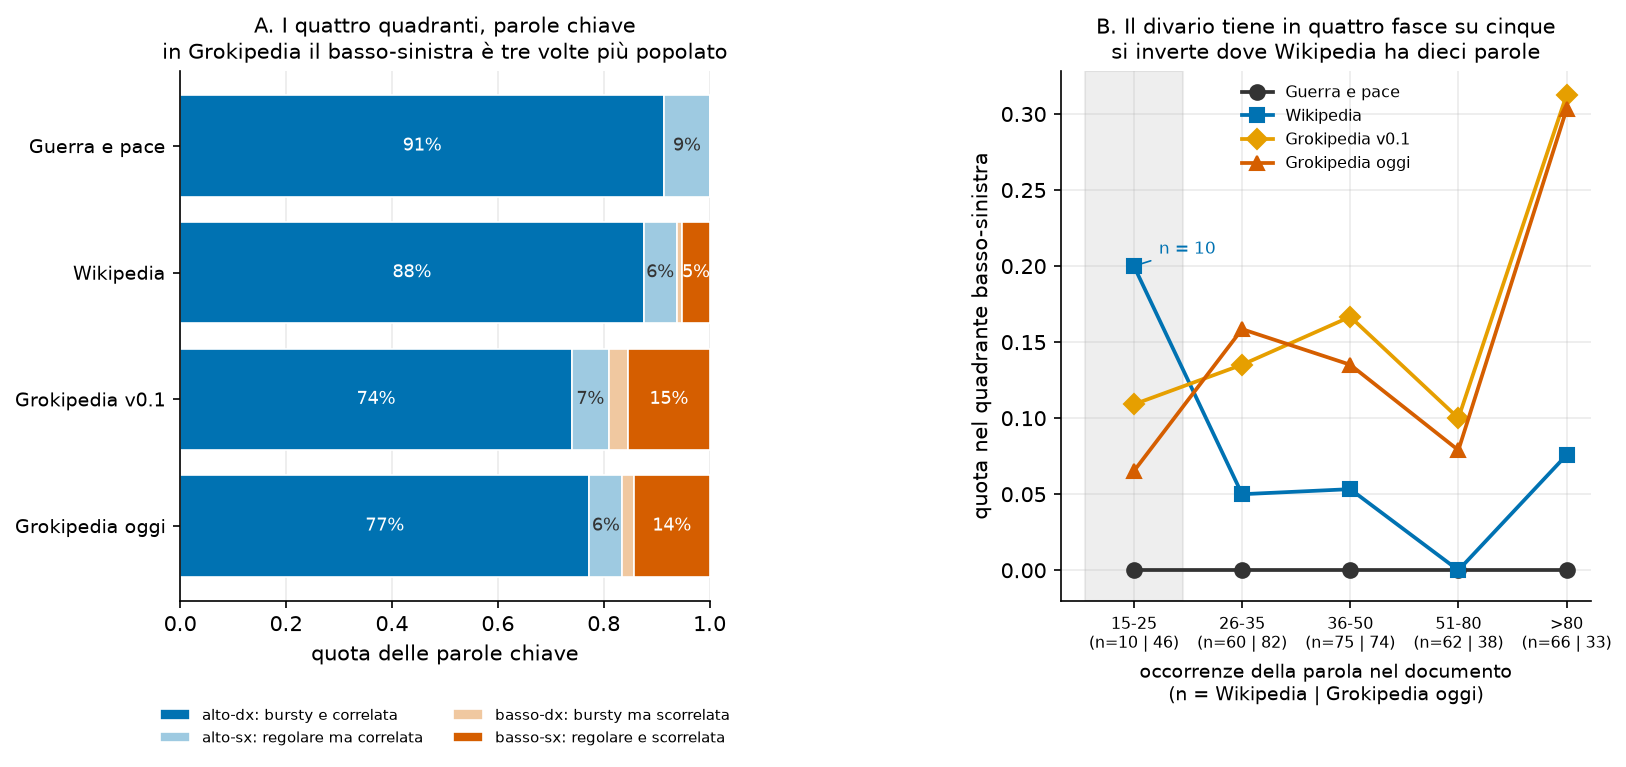
\includegraphics[width=\textwidth]{figure/cap5_quadranti.png}
  \caption{Lettura per quadranti del piano della
  Figura~\ref{fig:altmann-fig3}, sulle sole parole chiave. A: composizione per
  quadrante, un corpus per riga; le quote sotto il $5\%$ non sono etichettate. B:
  quota di parole chiave nel quadrante in basso a sinistra, separando le parole
  per numero di occorrenze nel documento; sotto ciascuna fascia è indicato
  quante parole chiave vi cadono in Wikipedia e in Grokipedia. Il divario tiene
  in quattro fasce su cinque e si inverte nella più bassa, dove Wikipedia ne ha
  dieci in tutto e la fascia è ombreggiata per segnalarlo.}
  \label{fig:quadranti}
\end{figure}

\paragraph{Un effetto di scala da neutralizzare.} Le voci di Grokipedia hanno
frasi sensibilmente
più lunghe di quelle di Wikipedia: $4.38$ frasi ogni mille caratteri contro
$6.92$. Poiché in questo capitolo il tempo è contato in caratteri, la scala
degli intervalli $\tau$ non è la stessa nei due corpora, e un testo con frasi
più lunghe tende ad avere intervalli più lunghi anche a parità di struttura
tematica. Il coefficiente di variazione è un rapporto e non risente di una
dilatazione uniforme dell'asse, ma la dilatazione qui non è uniforme, perché
agisce solo sui livelli definiti su unità linguistiche. Il
§\ref{sec:entropia-intervalli} introduce la misura che elimina il problema;
fino a quel punto il divario va considerato provvisorio.

Il riferimento letterario, infine, non è appaiato per argomento con nessuno dei
tre corpora enciclopedici: entra nei confronti come livello medio e non nei test
appaiati.

% ---------------------------------------------------------------------
\section{Quale meccanismo genera la correlazione}
\label{sec:decomposizione}

Sapere che un testo ha correlazioni a lungo raggio non dice da dove esse
vengano. Il §\ref{sec:null} ha introdotto i due null model che separano le due
origini possibili e la quota di burstiness $q$ della~\eqref{eq:quota}, che vale
circa uno quando la correlazione è interamente spiegata dalla distribuzione
degli intervalli, e circa zero quando è invece l'ordine in cui le occorrenze si
susseguono a produrla.

Il primo pannello della Figura~\ref{fig:decomposizione} riporta $q$ ai quattro
livelli. Sulle lettere il valore è negativo in tutti e quattro i corpora, da
$-0.06$ su Wikipedia a $-0.19$ su Grokipedia v0.1: le lettere sono correlate,
come mostra il $\hat\gamma$ maggiore di uno, ma non sono \emph{bursty}, e la
correlazione viene interamente dall'ordine. Sulle parole chiave il valore sale a
$0.89$ sul romanzo, $0.77$ su Wikipedia, $0.70$ sulla v0.1 e $0.74$ sulla
versione attuale di Grokipedia: qui quasi tutta la correlazione è già contenuta nella
distribuzione degli intervalli. I due livelli intermedi interpolano fra i due
regimi in modo ordinato.

La dissociazione fra il livello dei caratteri e quello del contenuto, che
in~\cite{altmann2012} è osservata su romanzi, si ritrova quindi identica nella
prosa enciclopedica e anche nella prosa generata. Il secondo pannello mostra la
stessa cosa in termini di esponenti: le curve piene sono $\hat\gamma$ e quelle
tratteggiate $\hat\gamma_{A2}$, e la distanza verticale fra le due è il
contributo dell'ordine delle occorrenze. Sulle lettere le due curve sono
separate e la tratteggiata sta all'unità; sulle parole chiave si avvicinano e
salgono insieme.

I valori dei tre corpora enciclopedici sono però troppo vicini perché la
differenza sia interpretabile: fra Wikipedia e Grokipedia vale $0.03$ alla
lunghezza di lavoro e cambia segno a quella di controllo del
§\ref{sec:robustezza-neff}. I dati non consentono quindi di attribuire ai due
corpora un'origine diversa della correlazione, ma soltanto un'intensità diversa.

Sulla riga dei controlli appaiati per Grokipedia, infine, la quota è stimabile
solo su $6$ documenti su $39$ per la versione v0.1 e su $8$ per quella
attuale. La ragione non è un difetto della stima ma la grandezza stessa: $q$
ha $\hat\gamma - 1$ al denominatore, e viene calcolata soltanto dove quel
denominatore supera $0.05$, perché sotto quella soglia il rapporto è dominato
dall'errore. A quel livello i documenti di Grokipedia hanno $\hat\gamma$
mediano pari a $1.003$ per la v0.1 e $1.015$ per la versione attuale, contro
$1.091$ di Wikipedia: le loro sequenze di controllo sono essenzialmente
scorrelate, e non c'è alcuna correlazione da decomporre nelle due origini.
L'esclusione è quindi essa stessa un dato, perché è il livello in cui il testo
generato si avvicina di più al caso, ma il valore di $q$ che sopravvive sui
pochi documenti restanti riguarda proprio quelli in cui una correlazione c'è,
e non va letto come una misura del corpus.

\begin{figure}[htbp]
  \centering
  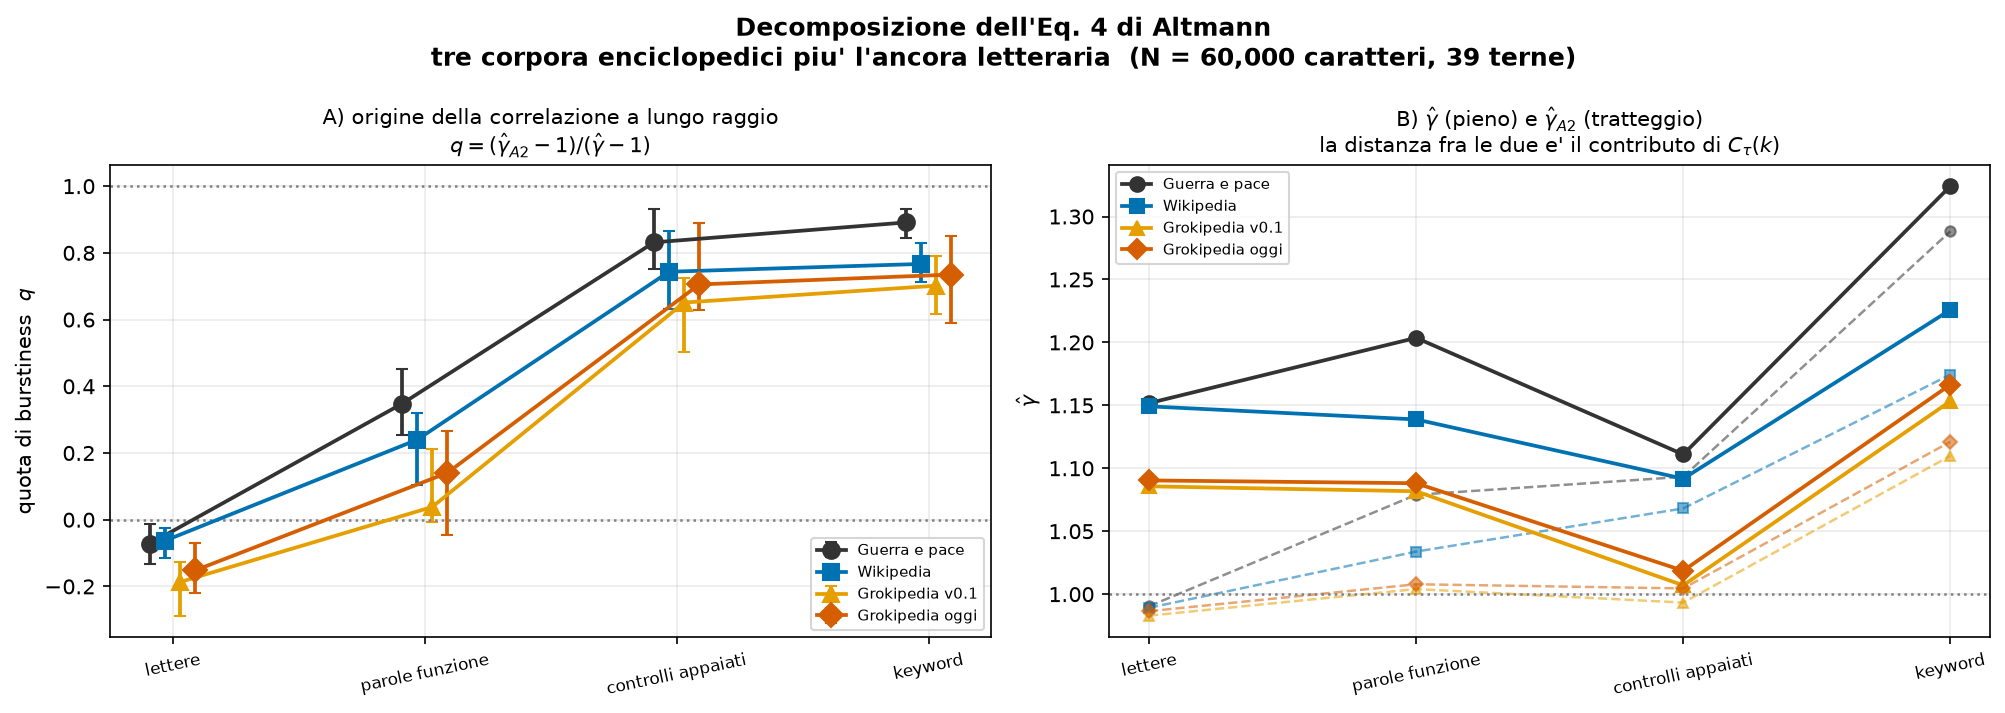
\includegraphics[width=\textwidth]{figure/cap5_decomposizione_eq4.png}
  \caption{Decomposizione della correlazione nelle sue due origini. A: quota
  $q$ della~\eqref{eq:quota} ai quattro livelli linguistici, con intervalli di
  confidenza; $q \simeq 0$ indica correlazione dovuta all'ordine delle
  occorrenze, $q \simeq 1$ correlazione dovuta alla distribuzione degli
  intervalli. B: esponente $\hat\gamma$ (linea piena) e $\hat\gamma_{A2}$
  (tratteggiata) agli stessi livelli; la distanza fra le due curve è il
  contributo della correlazione fra intervalli successivi.}
  \label{fig:decomposizione}
\end{figure}

% ---------------------------------------------------------------------
\section{La coda della distribuzione degli intervalli}
\label{sec:coda-risultati}

Il §\ref{sec:coda} ha osservato che la relazione fra esponente di coda e
esponente di correlazione, nella forma in cui compare in~\cite{altmann2012},
presuppone una distribuzione degli intervalli di cui la coda non viene misurata
ma assunta. Qui la coda viene stimata direttamente, adottando il modello
troncato
\begin{equation}
  p(\tau) \;\sim\; \tau^{-\mu}\,e^{-\tau/\tau_c}
  \label{eq:coda-troncata}
\end{equation}
e determinando $\mu$ e $\tau_c$ per massima verosimiglianza, con intervalli di
confidenza di profilo.

L'analisi della coda comprende, oltre ai quattro livelli usati nel resto del
capitolo, due livelli sub-lessicali aggiuntivi tenuti come diagnostica, le
vocali e gli spazi, per un totale di ventiquattro celle. Il primo risultato
riguarda la forma stessa della distribuzione: il confronto di verosimiglianza
fra la~\eqref{eq:coda-troncata} e una legge di potenza pura rifiuta
quest'ultima in tutte e ventiquattro, con significatività numericamente
indistinguibile da zero. La coda esiste, ma è tagliata.

Il primo pannello della Figura~\ref{fig:coda} riporta $\mu$ ai quattro livelli.
La banda verde segna la regione $2 < \mu < 3$ entro cui la~\eqref{eq:eq8} è
derivata assumendo una legge di potenza pura. Che le stime vi cadano dentro o
fuori non dice nulla sulla convergenza dei momenti: nella
~\eqref{eq:coda-troncata} il taglio li rende finiti per qualunque $\mu$, e il
rifiuto della potenza pura in tutte e ventiquattro le celle toglie il
presupposto sotto cui la banda avrebbe quel significato. Resta un riferimento
utile perché è la regione in cui il paper colloca il proprio valore assunto.
I simboli grigi segnalano le celle in cui il fit degenera in un
esponenziale puro e $\mu$ non è interpretabile, e le linee di collegamento le
saltano. Sono sette celle su sedici: tutti e quattro i corpora sul livello delle
lettere, e i tre corpora enciclopedici su quello delle parole funzione.

Alle parole funzione il romanzo è l'unico dei quattro il cui fit non degenera,
con $\tau_c = 5.3$ contro $1.7$--$1.9$: le sue parole funzione conservano un
tratto di coda a legge di potenza che negli altri tre corpora non esiste, e a
quel livello il coefficiente di variazione dà lo stesso quadro, $1.19$ contro
valori fra $0.97$ e $1.03$ indistinguibili da un processo di Poisson.

Sarebbe naturale leggerlo come una differenza di genere, e il controllo non lo
conferma. Ripetendo la stessa procedura sui tre romanzi inglesi impiegati come
controllo in questo capitolo, il fit sulle parole funzione degenera su
\emph{Moby Dick} ($\tau_c = 1.7$, esattamente il valore dei corpora
enciclopedici) e su \emph{David Copperfield} ($\tau_c = 2.8$), e sopravvive per
poco su \emph{Middlemarch} ($\tau_c = 3.2$); il coefficiente di variazione dà
$1.03$, $1.09$ e $1.08$, cioè valori compresi fra Wikipedia e
\emph{Guerra e pace} e nel primo caso identici a quelli enciclopedici. A questo
livello l'eccezione è quindi del testo e non del genere, come il
§\ref{sec:tre-corpora} osserva anche sul livello delle parole chiave. Il confronto fra i quattro
corpora resta perciò leggibile soltanto sulle parole chiave, dove i valori
stanno fra $1.76$ e $2.37$; sui controlli appaiati tutti e quattro i fit sono al
limite della degenerazione e gli intervalli di confidenza superano l'unità di
ampiezza.

Il confronto con~\cite{altmann2012} chiude qui un cerchio. In quel lavoro $\mu$
non viene stimato ma assunto: per costruire il limite inferiore di $\hat\gamma$
della propria Figura~3 gli autori adottano il valore $\mu = 2.4$. La stima
diretta condotta qui lo colloca dentro l'intervallo di confidenza di tutti e tre
i corpora enciclopedici, e a tre centesimi dal valore centrale di Wikipedia. Il
parametro che quel lavoro doveva postulare risulta dunque misurabile, e il
valore postulato corretto. Il confronto è legittimo perché $\mu$ designa in
entrambi i casi la pendenza della coda nella regione in cui la legge di potenza
vale; ciò che cambia è che qui quella regione è delimitata da un $\tau_c$
stimato anziché estesa all'infinito, e il capoverso seguente misura quanto la
differenza di modello sposti il numero.

Il corpus letterario fa eccezione, con $\mu = 1.76$ e intervallo di confidenza
$[1.40, 2.08]$, e su questo servono due precisazioni, perché il valore cade
sotto la banda $2 < \mu < 3$ entro cui la~\eqref{eq:eq8} è derivata. La prima
è che non è una particolarità di \emph{Guerra e pace}: ripetendo l'intera
procedura su tre altri romanzi inglesi, segmentati e misurati allo stesso
modo, si ottiene $1.51$ su \emph{Moby Dick}, $2.10$ su \emph{Middlemarch} e
$1.96$ su \emph{David Copperfield}, tutti sotto il valore di Wikipedia a ogni
quantile di $x_{\min}$ dall'ottantesimo in su. È un tratto della prosa
letteraria, non del testo scelto, ed è lo stesso fatto che il coefficiente di
variazione registra come burstiness massima: coda più pesante significa
esponente più piccolo.

La seconda è che il valore dipende dal modello con cui lo si stima. Sotto il
modello troncato adottato qui la banda $2 < \mu < 3$ non ha ruolo, perché il
taglio rende media e varianza finite per qualunque $\mu$; sotto il modello a
potenza pura, che è quello di~\cite{altmann2012}, lo stimatore di massima
verosimiglianza sugli stessi dati dà $2.49$ per il corpus letterario, dentro la
banda e a nove centesimi dal valore assunto nel paper. I due numeri non sono in
conflitto: descrivono la stessa coda sotto ipotesi diverse, e la scelta fra le
due è decisa dal rapporto di verosimiglianza, che rifiuta la potenza pura. La
misura non contraddice dunque il valore postulato in quel lavoro; ne circoscrive
il modello.

\begin{figure}[htbp]
  \centering
  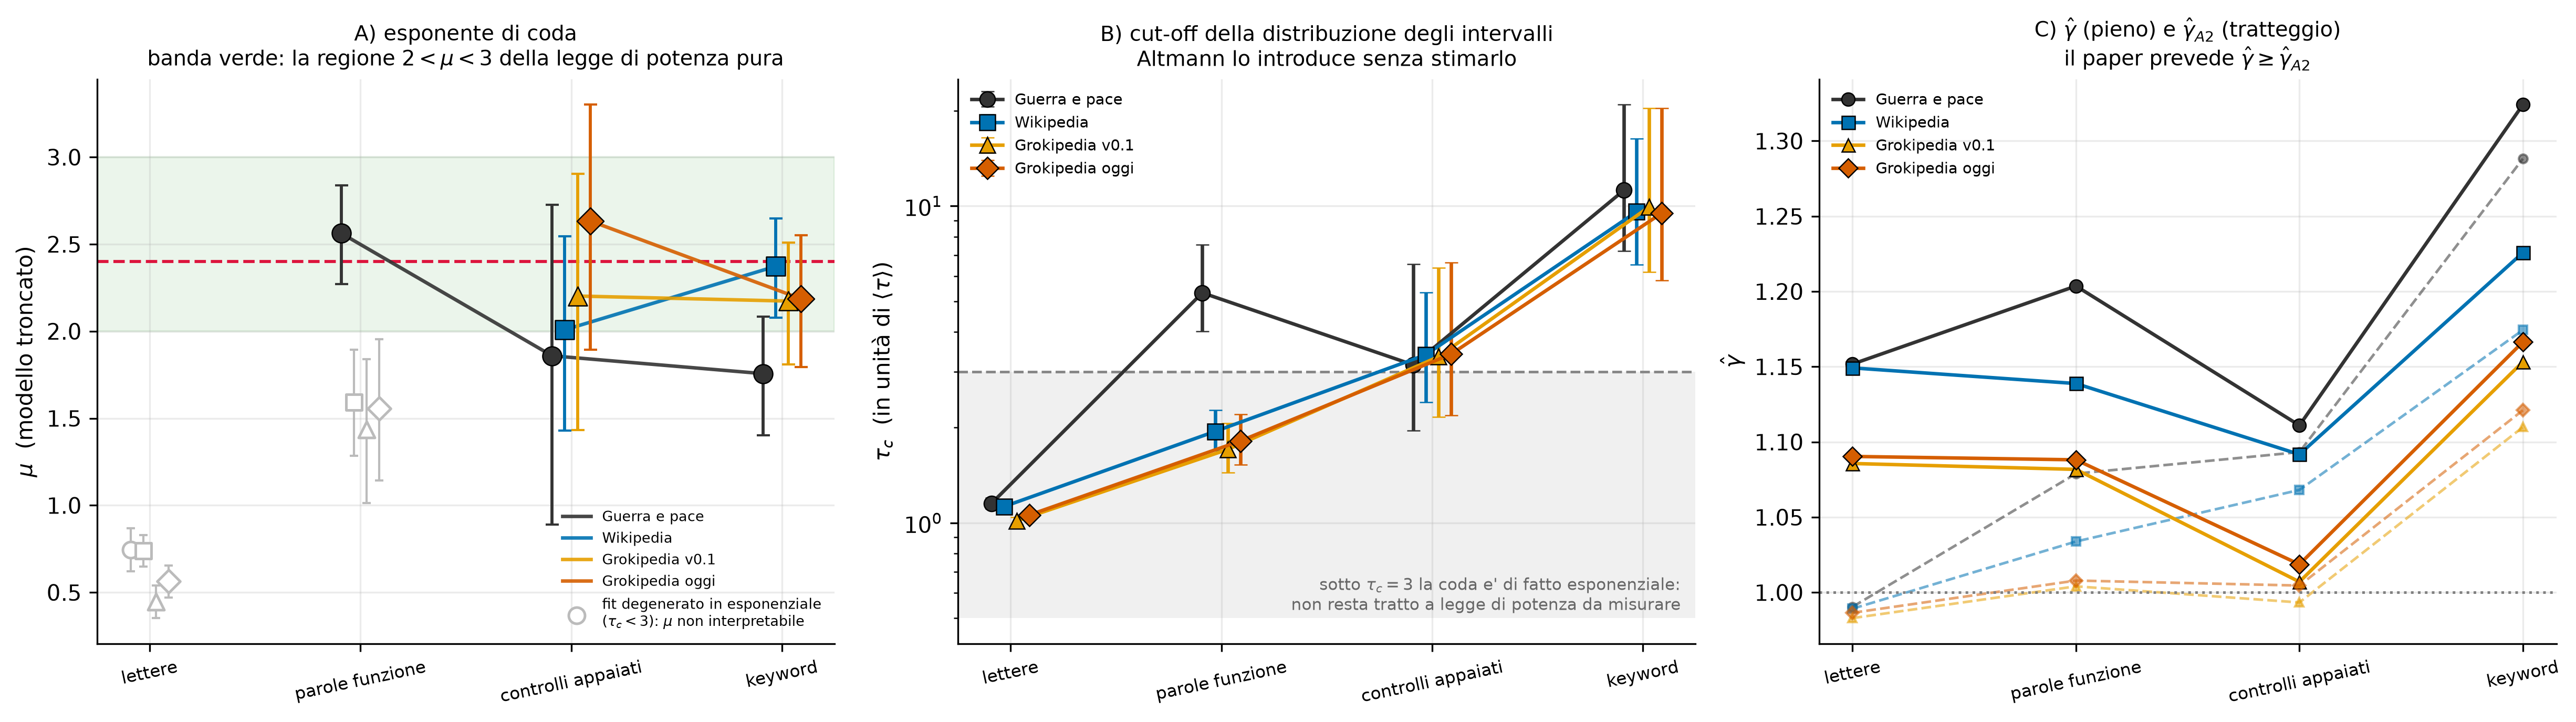
\includegraphics[width=\textwidth]{figure/cap5_esponente_coda.png}
  \caption{Stima diretta della coda della distribuzione degli intervalli. A:
  esponente $\mu$ della~\eqref{eq:coda-troncata} ai quattro livelli, con
  intervalli di confidenza di profilo; la banda verde è la regione $2<\mu<3$ in
  cui è derivata la~\eqref{eq:eq8} per la legge di potenza pura, mentre sotto il
  modello troncato adottato qui i momenti restano finiti per qualunque $\mu$ e
  la banda va letta come riferimento alla letteratura; i simboli grigi sono le
  celle in cui il fit degenera in un esponenziale e $\mu$ non è interpretabile,
  che le linee di collegamento saltano. B: cut-off
  $\tau_c$ agli stessi livelli, in unità dell'intervallo medio e con intervalli
  di confidenza di profilo; sotto la soglia tratteggiata non resta tratto a legge
  di potenza da misurare. C: $\hat\gamma$ (pieno) contro $\hat\gamma_{A2}$
  (tratteggiato) ai quattro livelli. La~\eqref{eq:disug1} è rispettata in tutte
  le celle: la curva piena sta sempre sopra la tratteggiata.}
  \label{fig:coda}
\end{figure}

\paragraph{Perché $\mu$ non serve a confrontare i corpora.}
I quattro valori non vanno però usati per ordinare i corpora, e la
Figura~\ref{fig:verosimiglianza} mostra perché: $\mu$ e $\tau_c$ sono
fortemente correlati, cosicché le regioni di confidenza congiunte sono creste
allungate anziché ellissi compatte e quelle dei tre corpora enciclopedici si
sovrappongono quasi interamente. A ciò si aggiunge la dipendenza dal punto in
cui si decide che la coda cominci: spostando $x_{\min}$ dal settantacinquesimo
al novantacinquesimo percentile $\mu$ passa da $1.65$ a $2.63$ su Wikipedia, una
variazione maggiore di ogni differenza fra corpora, e le curve si incrociano.

Di questa analisi non resta perciò un ordinamento fra corpora. Restano due
risultati, entrambi insensibili alla posizione esatta lungo la cresta: la legge
di potenza pura è rifiutata ovunque, e il cut-off cresce in modo ordinato
salendo nella gerarchia linguistica. Il cut-off è previsto
da~\cite{altmann2012} come conseguenza della discesa lungo quella stessa
gerarchia, e la sua esistenza è qui verificata invece che assunta.

\begin{figure}[htbp]
  \centering
  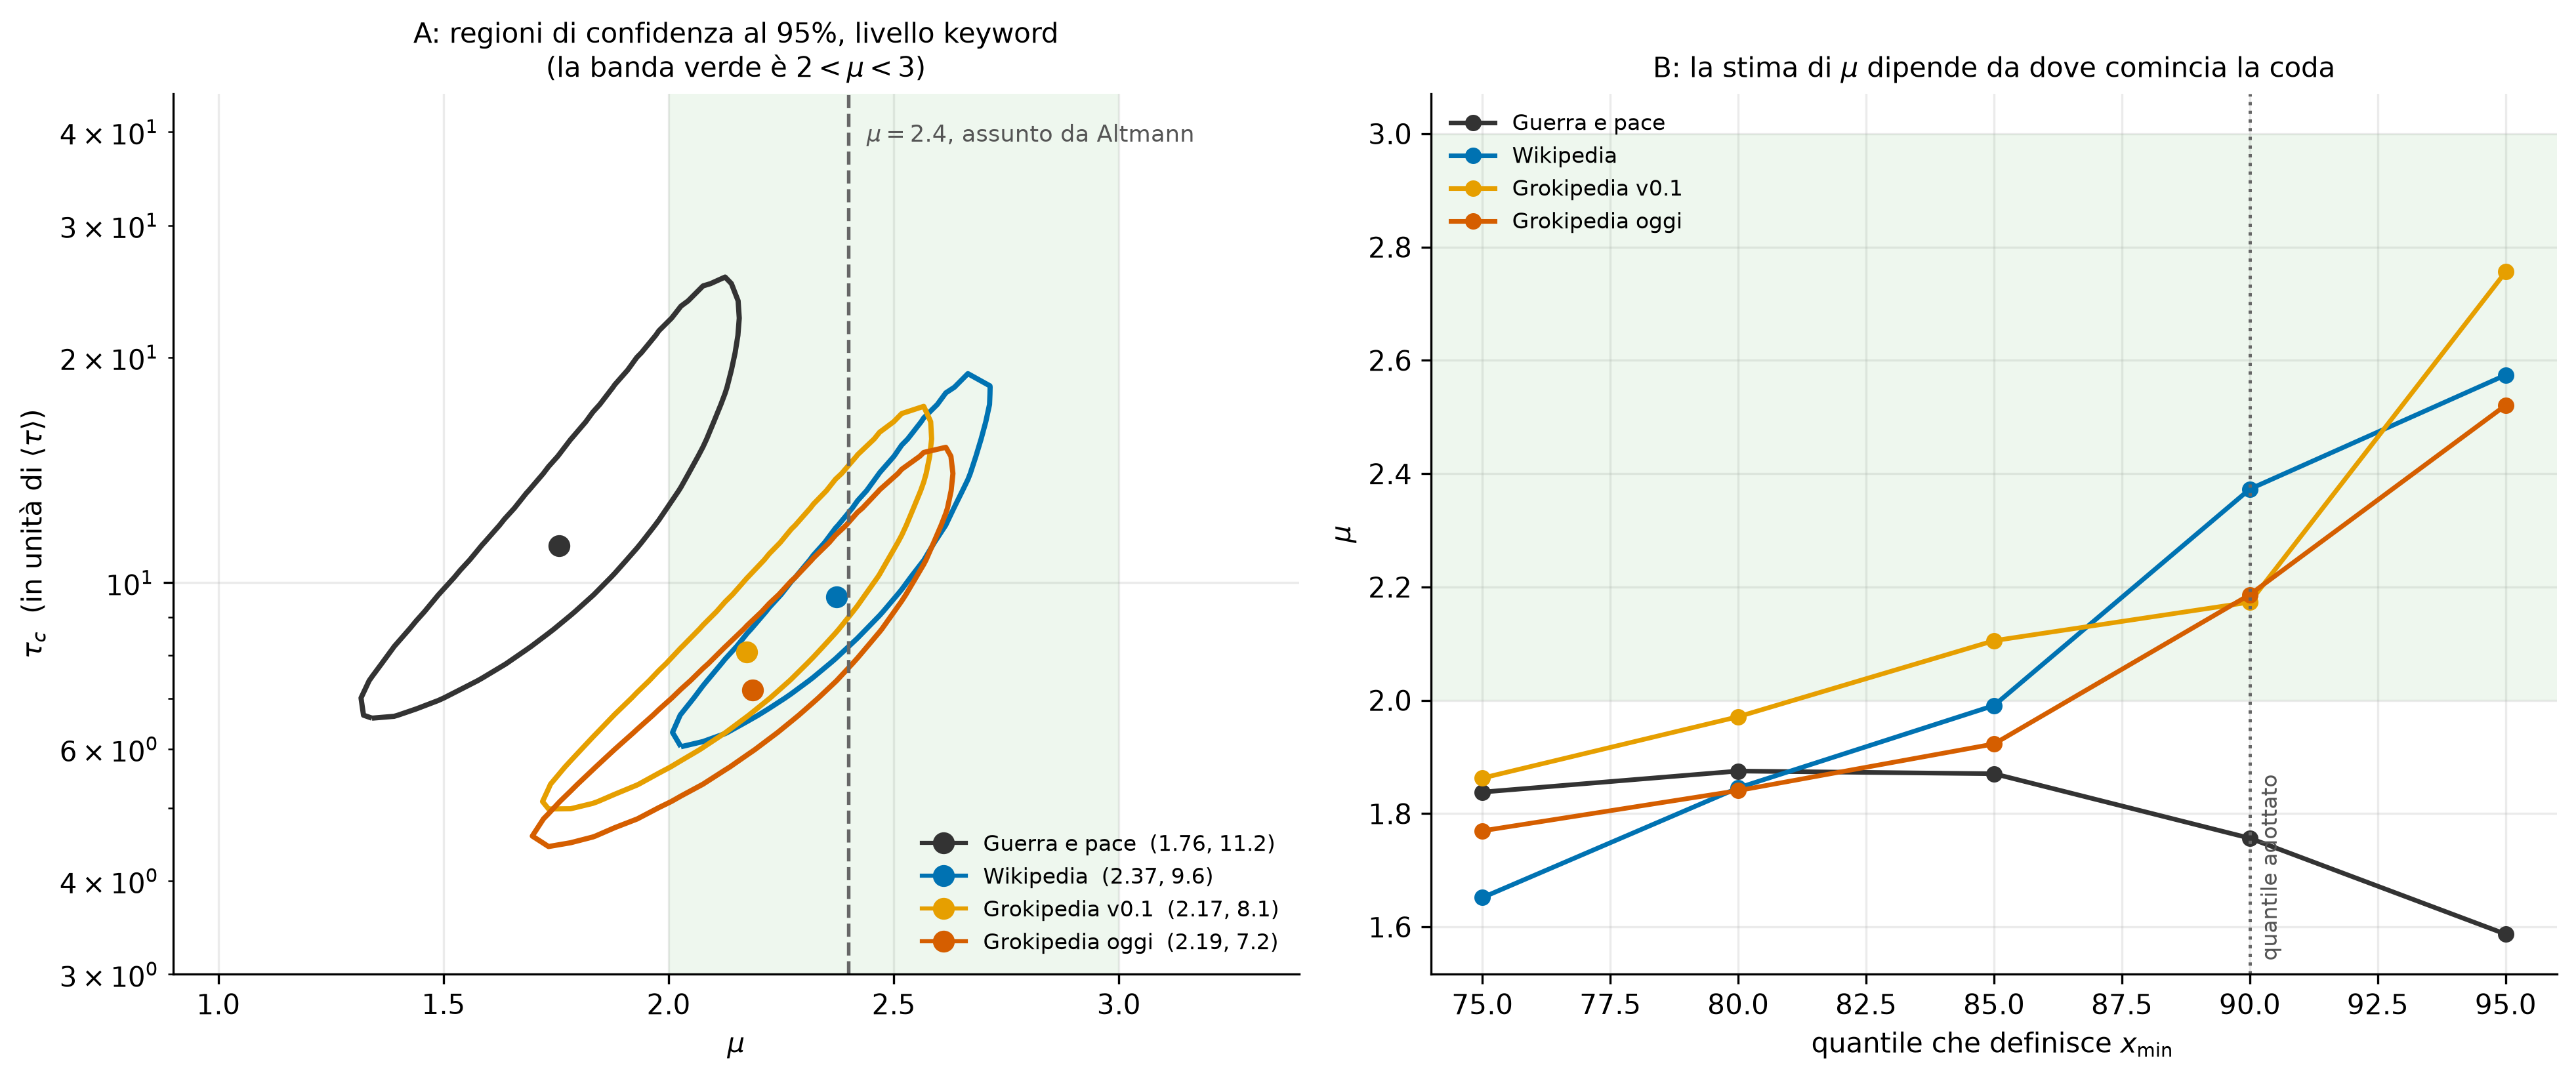
\includegraphics[width=\textwidth]{figure/cap5_verosimiglianza_coda.png}
  \caption{Perché l'esponente di coda non discrimina fra i corpora. A: regioni
  di confidenza congiunte al $95\%$ nel piano $(\mu, \tau_c)$ sul livello delle
  parole chiave, con $x_{\min}$ al novantesimo percentile; l'allungamento delle
  regioni è la correlazione fra i due parametri, e la linea tratteggiata è il
  valore $\mu = 2.4$ assunto in~\cite{altmann2012}. B: stima di $\mu$ al variare
  del quantile che definisce $x_{\min}$; le quattro curve si incrociano, cosicché
  l'ordinamento fra corpora dipende da quella scelta.}
  \label{fig:verosimiglianza}
\end{figure}

\paragraph{Il cut-off e la finestra di osservazione.} Il secondo pannello
della Figura~\ref{fig:coda} riporta $\tau_c$ ai quattro livelli, con
intervalli di confidenza di profilo. È l'altra metà di ciò
che~\cite{altmann2012} introduce senza stimare: il cut-off vi compare come
conseguenza necessaria della discesa nella gerarchia, ma non gli viene mai
assegnato un valore. Cresce in modo ordinato salendo nella gerarchia: circa
$1.1$ volte l'intervallo medio sulle lettere, dove la coda è di fatto già
esponenziale, $3.2$--$3.4$ sui controlli appaiati e $9.5$--$11.2$ sulle parole
chiave. La separazione fra i due livelli superiori è netta. Fra i quattro
corpora, invece, gli intervalli di confidenza si sovrappongono ampiamente:
neppure il cut-off ordina i corpora, e la sola cella in cui la separazione è
significativa è quella delle parole funzione del romanzo, discussa sopra.

Anche $\tau_c$ va poi letto come descrittore relativo alla lunghezza di analisi.
Ripetendo la stima sul romanzo a lunghezze crescenti, da \num{30000} a
\num{480000} caratteri, $\tau_c$ passa da $13.5$ a $94.7$: un fattore sette a
fronte di un fattore sedici sulla finestra, con un andamento non monotono che
scende prima di risalire. Il taglio non è dunque un puro artefatto, perché non
scala proporzionalmente alla finestra, ma non è nemmeno una lunghezza intrinseca
del testo. Sulla stessa serie $\mu$ si stabilizza attorno a $2.0$ alle finestre
maggiori, contro l'$1.76$ misurato alla lunghezza di lavoro: entrambi i
parametri descrivono la coda \emph{a quella lunghezza}, coerentemente con la
regola del §\ref{sec:lunghezza}.

\paragraph{Lo stimatore di Hill.} Dà sistematicamente valori più alti, $2.49$ sul
romanzo contro $1.76$ e circa $3.0$ sugli altri tre corpora contro
$2.2$--$2.4$, perché assume una legge di potenza pura su tutta la coda.
L'assenza di un plateau nel suo grafico diagnostico è ciò che ha motivato
l'adozione del modello troncato, e i suoi valori sono riportati solo a quel
titolo.

% ---------------------------------------------------------------------
\section{Entropia degli intervalli}
\label{sec:entropia-intervalli}

L'effetto di scala dichiarato nel §\ref{sec:appaiato} richiede una misura che
non risenta della lunghezza media delle frasi. È la ragione per cui il
§\ref{sec:entropia-intervalli-def} ha introdotto l'entropia degli intervalli
$J$ della~\eqref{eq:entropia-intervalli}: il logaritmo la rende invariante per
dilatazione dell'asse, cosicché frasi mediamente più lunghe non la spostano, e
la sottrazione del termine poissoniano ne cancella il bias. La grandezza è
risultata calcolabile su \num{5343} sequenze su \num{5617}, il $95\%$ del
totale.

\paragraph{Perché la misura è legittima.}
Trattandosi di una grandezza introdotta qui, la sua adozione va giustificata su
quello che fa e non su un precedente. I due ingredienti sono però entrambi
standard: l'entropia differenziale stimata per spaziature d'ordine è lo
stimatore di~\cite{vasicek1976}, e il confronto di una statistica osservata con
il valore che essa assume su un processo di Poisson di pari intensità è la
costruzione con cui in letteratura si misura la regolarità di una sequenza di
eventi, la stessa su cui poggiano la~\eqref{eq:cv} e il coefficiente
di~\cite{goh2008} usati nel resto del capitolo. Ciò che $J$ aggiunge è
l'invarianza per dilatazione, che nessuna delle due possiede e che serve qui per
una ragione specifica. Il §\ref{sec:entropia-intervalli-def} argomenta perché
debba funzionare; la validazione empirica è alla fine di questa sezione, dove la
stessa parola misurata a lunghezze diverse sposta il coefficiente di variazione
di un fattore tre e $J$ di due decimi di bit.

\paragraph{Che cosa riportano i tre pannelli.}
Il primo pannello della Figura~\ref{fig:entropia} mostra il rapporto fra $J$ e
il coefficiente di variazione sulle parole chiave. Le due misure sono
correlate, come atteso, ma la relazione non è biunivoca: a parità di
coefficiente di variazione i punti dei diversi corpora occupano fasce di $J$
diverse, il che è precisamente ciò che rende utile la seconda misura.

Il secondo pannello riporta $J$ ai quattro livelli. Sulle lettere i quattro
corpora coincidono attorno a $-0.20$, e sulle parole funzione i tre corpora
enciclopedici scendono insieme attorno a $-0.29$, con il romanzo che resta a
$-0.19$: valori negativi indicano intervalli più regolari di un
processo di Poisson. Sui due livelli superiori i corpora si separano, e sulle
parole chiave i corpora umani stanno sopra il valore poissoniano e quelli
generati vi si appoggiano: $J$ vale $+0.061$ sul romanzo e $+0.092$ su
Wikipedia, contro $-0.001$ su Grokipedia v0.1 e $-0.011$ sulla versione
attuale, questi ultimi due indistinguibili da zero. Le due enciclopedie generate
si collocano dunque sul valore poissoniano, mentre quella umana ne sta sopra:
gli intervalli fra parole chiave di Grokipedia non sono più regolari del caso,
semplicemente non sono più \emph{bursty} di esso. Il terzo pannello riporta la
distribuzione per documento e mostra che la separazione, pur con code
sovrapposte, riguarda l'intero corpus e non alcune voci.

\paragraph{La coda inferiore è fatta di soggetti di voce.}
La coda inferiore di quel pannello merita però un controllo, perché il cambio
di segno è ciò su cui l'affermazione precedente poggia. Le sequenze con $J$
più basso sono parole chiave a pieno titolo, nomi propri e non lessico di
servizio sfuggito alla lista chiusa, ma sono quasi tutte la stessa cosa: il
soggetto della voce. Fra le venti sequenze di $J$ minore, in Grokipedia
quattordici sono il soggetto dell'articolo, e in Wikipedia diciotto:
\emph{churchill}, \emph{newton}, \emph{paris}, \emph{freud}, \emph{mandela}. È
il fenomeno del §\ref{sec:tre-corpora}, che $J$ registra come gli altri
indicatori, e non è un difetto della classificazione.

Ha però una conseguenza sul cambio di segno. Escludendo i soggetti delle voci,
$54$ sequenze su $273$ in Grokipedia e $57$ in Wikipedia, tutti e tre i
corpora enciclopedici passano sopra il valore poissoniano: $+0.175$ su
Wikipedia e $+0.070$ su Grokipedia. Il divario appaiato sopravvive, $-0.087$
bit con $p < 10^{-3}$, e con esso la conclusione del paragrafo; non sopravvive
invece la lettura per segno, perché il segno negativo di Grokipedia è prodotto
dai soggetti delle voci, che il §\ref{sec:tre-corpora} ha già mostrato essere
marcatori sintattici e non semantici. Ciò che distingue i due corpora è quanto
$J$ vale, non da che parte dello zero cade.

\paragraph{Il divario appaiato.}
I confronti appaiati confermano il divario: sulle parole chiave la differenza
mediana fra Grokipedia attuale e Wikipedia vale $-0.105$ bit e quella fra la
v0.1 e Wikipedia $-0.077$ bit, entrambe con significatività inferiore a
$10^{-3}$. Sulle lettere e sulle parole funzione, per contro, le differenze sono
positive e non significative. Poiché $J$ non risente della diversa lunghezza
delle frasi, questo risultato conferma il divario del §\ref{sec:appaiato}
senza risentire di quell'effetto, ed è il punto in cui la conclusione principale
del capitolo diventa difendibile.

\paragraph{Perché il divario è più ampio sui controlli.}
Il divario è però più ampio sui controlli appaiati, $-0.209$ bit, che sulle
parole chiave, e la ragione sta in che cosa siano quei controlli. Il controllo
di una parola chiave è la parola di frequenza più vicina fra quelle che restano
dopo aver tolto le parole chiave stesse, i nomi propri e le sei parole funzione
selezionate; poiché le parole chiave sono per costruzione le più frequenti del
loro tipo, ciò che resta a quelle frequenze è in larga parte lessico di
servizio. I controlli più ricorrenti sono infatti \emph{by}, \emph{from},
\emph{with} e \emph{as} in Wikipedia, e \emph{like}, \emph{but}, \emph{that} e
\emph{this} in Grokipedia. È il livello in cui il testo generato si distingue di
più: le sue parole di servizio sono distribuite quasi uniformemente,
$J = -0.165$, mentre quelle di Wikipedia conservano un residuo di
addensamento, $J = +0.053$.

\paragraph{Composizione e stile, in parti quasi uguali.}
Le due liste di controlli sono però diverse fra loro, e la differenza potrebbe
misurare quali parole vengono selezionate anziché come sono distribuite. Le due
cause si separano restringendo il confronto alle parole che compaiono fra i
controlli di entrambi i corpora. Sono ventisei, e dodici raggiungono almeno tre
voci per corpus. Su queste il divario resta: la differenza mediana di $J$ vale
$-0.091$ bit con $p = 0.043$, e le quattro parole più spostate sono
\emph{with} ($-0.060$ contro $-0.414$), \emph{as} ($+0.227$ contro $-0.106$),
\emph{this} ($-0.005$ contro $-0.301$) e \emph{from} ($+0.057$ contro $-0.225$).
Il divario fra le medie dei due corpora, $-0.218$ bit, si scompone dunque in
$-0.128$ attribuibili alla distribuzione delle stesse parole e $-0.091$ alla
diversa composizione delle due liste, cioè in parti quasi uguali. Il valore
differisce di un centesimo dal $-0.209$ citato sopra perché quello è la mediana
delle differenze voce per voce e questo la differenza fra le medie.

La parte attribuibile alla composizione ha un contenuto proprio. I controlli di
Wikipedia sono preposizioni e ausiliari legati alla struttura del periodo, come
\emph{by}, \emph{was}, \emph{with} e \emph{for}; quelli di Grokipedia sono in
prevalenza connettivi di discorso, come \emph{like}, \emph{but}, \emph{that} e
\emph{over}. La parte attribuibile alla distribuzione descrive invece un
meccanismo: in Wikipedia una preposizione come \emph{from} si addensa dove il
contenuto la richiede, in una sezione biografica più che in una tecnica, e i suoi
intervalli ereditano il ritmo delle sezioni; in Grokipedia la stessa parola
ricorre a cadenza quasi costante lungo tutto l'articolo. Il segno negativo di $J$
dice che quella cadenza è più regolare di quella di un processo casuale, non
soltanto meno addensata.

Una verifica interna conferma la lettura. Nei controlli di Wikipedia il $93\%$
delle parole appartiene alla lista chiusa e dà $J = +0.043$, mentre il restante
$7\%$ dà $+0.188$: la classe grammaticale della parola cambia il risultato. In
Grokipedia le due quote valgono $-0.151$ e $-0.182$, indistinguibili fra loro.
Nel testo generato la regolarità degli intervalli non dipende da che tipo di
parola si stia guardando, ed è la stessa compressione uniforme della variabilità
lessicale che il §\ref{sec:sintesi-cap5} indica come conclusione del capitolo,
osservata al livello in cui si manifesta con più forza.

\paragraph{Stabilità rispetto alla lunghezza di analisi.}
Una validazione indipendente riguarda la dipendenza dalla lunghezza. Passando
da \num{40000} caratteri al romanzo intero, il coefficiente di variazione della
parola \emph{prince} cambia di un fattore $3.08$, mentre il suo $J$ si sposta di
$0.21$ bit; per la parola \emph{pierre} il coefficiente cambia di un fattore
$3.49$ e $J$ di $0.08$ bit. I due numeri non sono direttamente confrontabili,
perché il coefficiente di variazione è un rapporto e $J$ un logaritmo: uno
spostamento di $0.21$ bit corrisponde a un fattore $2^{0.21} = 1.16$ sulla
dispersione efficace degli intervalli, e uno di $0.08$ bit a un fattore $1.06$.
Riportate alla stessa scala, le due derive stanno nel rapporto di $2.7$ e $3.3$
in favore di $J$. La nuova misura è dunque circa tre volte più stabile rispetto
alla lunghezza di analisi di quella che sostituisce, il che ne conferma
l'utilità al di là del problema specifico per cui era stata introdotta.

\begin{figure}[htbp]
  \centering
  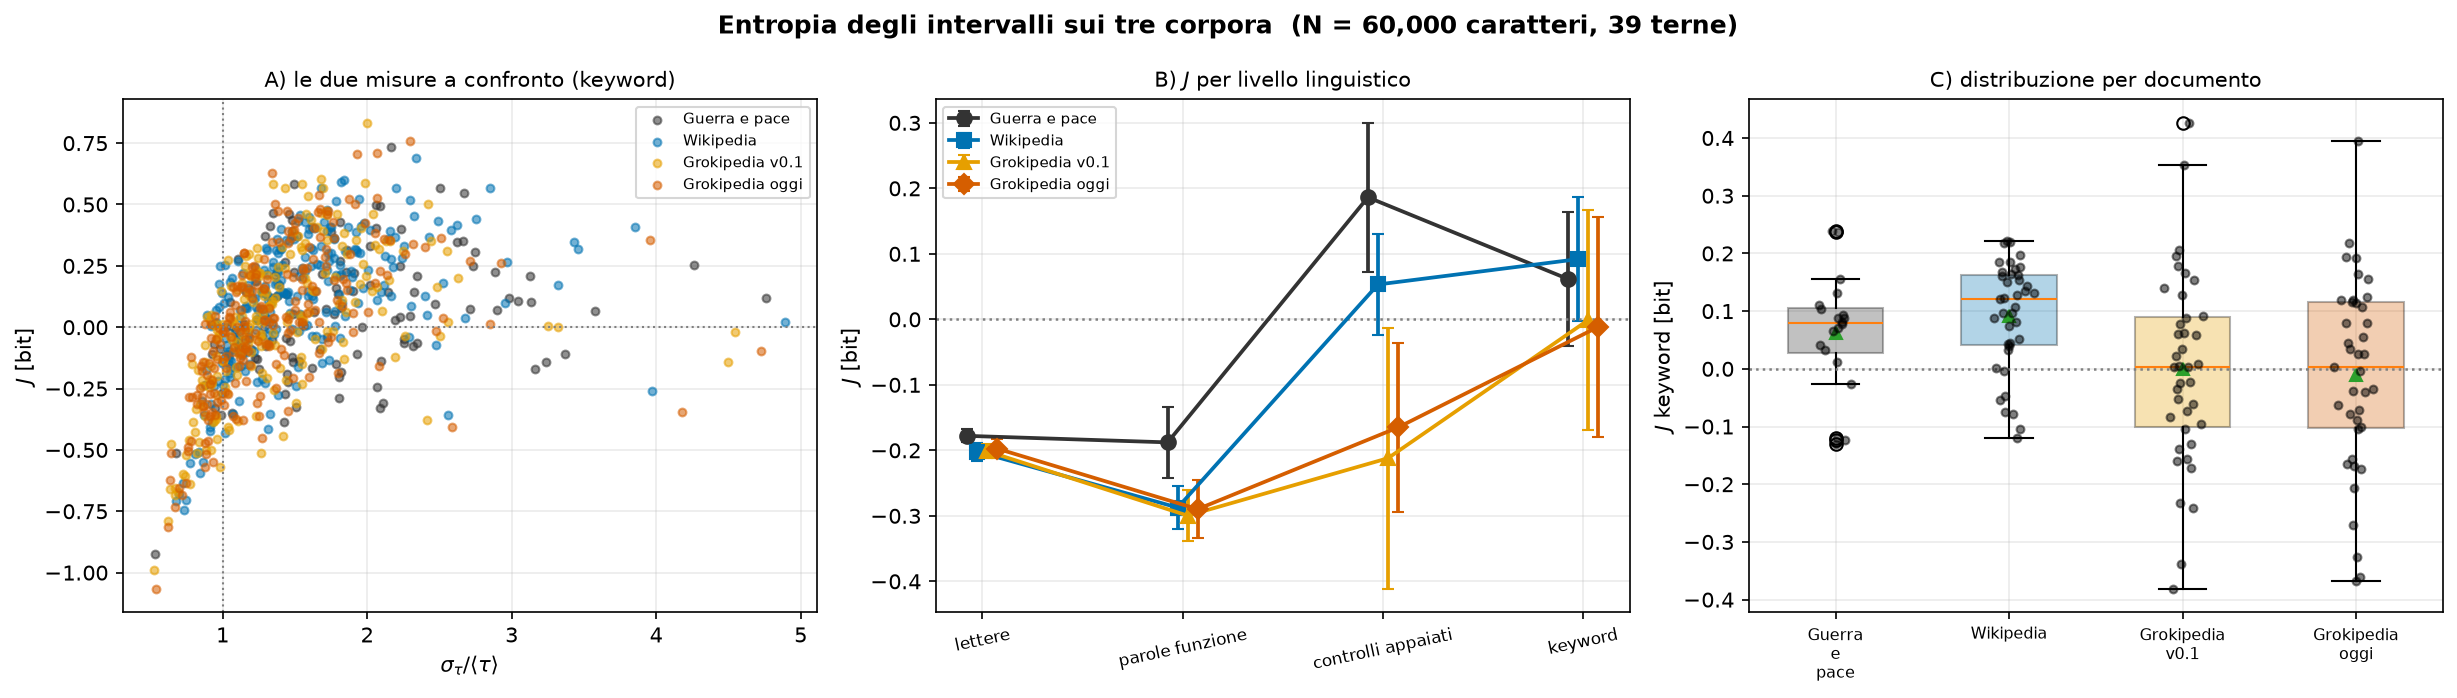
\includegraphics[width=\textwidth]{figure/cap5_entropia_intervalli.png}
  \caption{Entropia degli intervalli. A: relazione fra $J$ e coefficiente di
  variazione sulle parole chiave, un punto per sequenza. B: $J$ ai quattro
  livelli linguistici, con deviazioni standard fra testi; valori negativi
  indicano intervalli più regolari di un processo di Poisson. C: distribuzione
  di $J$ sulle parole chiave documento per documento. La misura è invariante per
  dilatazione dell'asse dei caratteri e non risente quindi della diversa
  lunghezza delle frasi nei due corpora enciclopedici.}
  \label{fig:entropia}
\end{figure}

% ---------------------------------------------------------------------
\section{Quanto pesa la definizione dei livelli lessicali}
\label{sec:effetto-stoplist}

Il paragrafo \emph{Come vengono separati i livelli lessicali} del
§\ref{sec:scelte} ha documentato l'estensione della lista chiusa di parole funzione da
\num{133} a \num{215} voci e la ragione per cui era necessaria. Questa sezione
riporta di quanto si spostano i risultati, perché lo spostamento non è
trascurabile e la scelta deve restare verificabile.

Il pannello A della Figura~\ref{fig:effetto-stoplist} riporta quali parole la
lista originaria lasciava passare fra le parole chiave di Grokipedia, e in
quante voci ciascuna: nell'elenco corrispondente di Wikipedia non ne compare
nessuna, e le sue sette parole sono distinte fra loro, ciascuna in una sola
voce.

\begin{table}[htbp]
  \centering
  \begin{tabular}{lcccc}
    \toprule
    & \multicolumn{2}{c}{lista originaria} & \multicolumn{2}{c}{lista estesa} \\
    \cmidrule(lr){2-3}\cmidrule(lr){4-5}
    & Wikipedia & Grok. oggi & Wikipedia & Grok. oggi \\
    \midrule
    keyword più bursty del controllo & $0.685$ & $0.630$ & $0.692$ & $0.740$ \\
    idem, su $\hat\gamma$ & $0.736$ & $0.663$ & $0.747$ & $0.791$ \\
    $\sigma_\tau/\langle\tau\rangle$ keyword & $1.530$ & $1.289$ & $1.536$ & $1.379$ \\
    divario appaiato, keyword & \multicolumn{2}{c}{$-0.230$} & \multicolumn{2}{c}{$-0.167$} \\
    divario appaiato, controlli & \multicolumn{2}{c}{$-0.122$} & \multicolumn{2}{c}{$-0.157$} \\
    $J$ keyword & $+0.086$ & $-0.069$ & $+0.092$ & $-0.011$ \\
    $\mu$ keyword & $2.38$ & $2.52$ & $2.37$ & $2.19$ \\
    quadrante basso-sinistra & $5.1\%$ & $24.5\%$ & $5.1\%$ & $14.3\%$ \\
    \bottomrule
  \end{tabular}
  \caption{Effetto della definizione dei livelli lessicali sui risultati del
  capitolo. Le righe dei divari appaiati riportano un solo valore perché
  misurano la differenza fra i due corpora. Le lettere e le parole funzione non
  compaiono perché nessuna parola cambia livello a quelle altezze: i loro valori
  coincidono a tutte le cifre riportate nel capitolo.}
  \label{tab:effetto-stoplist}
\end{table}

La Tabella~\ref{tab:effetto-stoplist} riporta il confronto. Tre risultati
cambiano in modo sostanziale. Il primo è il test interno: con la lista
originaria Grokipedia sembrava battere il proprio controllo appaiato meno spesso
di Wikipedia, e l'ordinamento fra i corpora appariva netto; con la lista estesa
l'ordine si inverte, e la differenza fra le due enciclopedie sparisce. Il
pannello B della figura mostra i due esiti sovrapposti. Il secondo è l'entropia
degli intervalli, il cui valore sulle parole chiave passa da $-0.069$ a
$-0.011$, cioè da un cambio di segno netto a uno indistinguibile da zero. Il
terzo è l'esponente di coda, che su Grokipedia scende da $2.52$ a $2.19$,
avvicinandosi a quello di Wikipedia anziché allontanarsene.

Restano invece stabili il divario appaiato complessivo, che si riduce da
$-0.230$ a $-0.167$ senza perdere significatività, il coefficiente di variazione
delle parole chiave, e l'intera decomposizione della~\eqref{eq:eq4}. Non si
muovono di una cifra, come è ovvio, i livelli delle lettere e delle parole
funzione.

La lezione metodologica vale al di là di questo caso. La distinzione fra
parole di contenuto e parole di servizio è la premessa dell'intero protocollo
di~\cite{altmann2012}, e viene qui operata da una lista chiusa che il paper
non specifica. Quando i corpora confrontati hanno abitudini lessicali diverse,
e un modello linguistico ne ha rispetto a un redattore umano, una lista
incompleta non introduce un rumore simmetrico: sposta sistematicamente in un
solo corpus il confine fra i due livelli, e produce un divario che non c'è.

\begin{figure}[htbp]
  \centering
  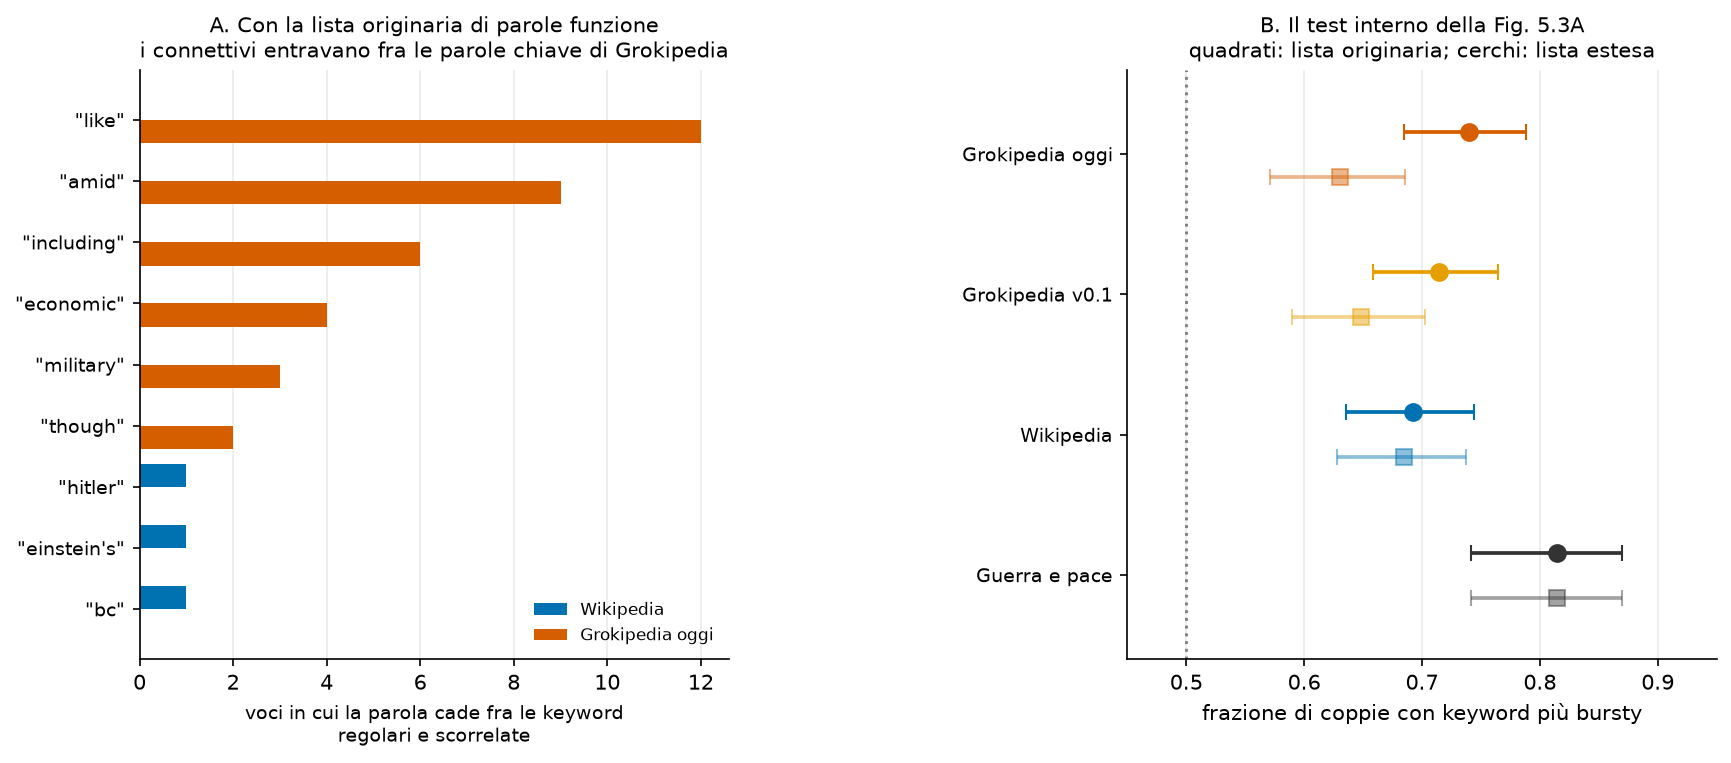
\includegraphics[width=\textwidth]{figure/cap5_effetto_stoplist.png}
  \caption{Effetto della definizione dei livelli lessicali. A: con la lista di
  funtori originaria, quali parole cadevano fra le parole chiave classificate
  come regolari e scorrelate, contate come numero di voci in cui ciò accadeva;
  le prime tre di Grokipedia sono connettivi, e in Wikipedia non compaiono. B:
  il test interno della Figura~\ref{fig:tre-corpora}A con le due
  classificazioni, quadrati per la lista originaria e cerchi per quella estesa,
  con intervalli di confidenza al $95\%$.}
  \label{fig:effetto-stoplist}
\end{figure}

% ---------------------------------------------------------------------
\section{Che cosa il testo generato non riproduce}
\label{sec:sintesi-cap5}

Il testo generato possiede correlazioni a lungo raggio, e ai livelli bassi della
gerarchia linguistica le possiede quasi nella stessa misura del testo umano:
sulle lettere i quattro corpora sono indistinguibili per coefficiente di
variazione, per entropia degli intervalli e per quota di burstiness, e sulle
parole funzione la differenza è piccola, benché significativa. Al livello delle parole il divario si apre, e vale più di un ordine
di grandezza rispetto a quello misurato sui caratteri.

Il divario non distingue però le parole che portano il contenuto dai controlli a
frequenza appaiata. I due valori sono quasi uguali alla lunghezza di lavoro,
$-0.157$ e $-0.167$, e si invertono a quella di controllo
(§\ref{sec:robustezza-neff}); e il test che chiede se la parola chiave superi il
proprio controllo \emph{dentro lo stesso testo} dà a Grokipedia un esito pari a
quello di Wikipedia, anzi lievemente migliore. Il meccanismo descritto
in~\cite{altmann2012} è dunque presente nel testo generato, e con la stessa
efficacia: ciò che manca è l'ampiezza con cui le parole, di contenuto e non, si
addensano.

Non si tratta dunque di una persistenza tematica assente, perché la distinzione
fra parole tematiche e parole ordinarie il modello la produce; si tratta di una
compressione uniforme della variabilità lessicale, che riduce la burstiness di
tutte le parole senza alterare il rapporto fra le une e le altre. Vale ancora la
distinzione posta nel §\ref{sec:intro-linguaggio} fra riprodurre le proprietà
statistiche del linguaggio e riprodurre il meccanismo che le genera, ma
applicata a un livello più basso di quanto la prima lettura suggerisse.

Ciò che il capitolo misura è la distanza fra due enciclopedie appaiate titolo
per titolo, e null'altro. Il deficit è osservato su Grokipedia, cioè su un unico
sistema generativo, in un unico dominio e in una sola lingua: nulla di quanto
riportato qui stabilisce che sia una proprietà dei modelli linguistici in
generale anziché di quel sistema. Il Capitolo~\ref{cap:risultati1} non offre un
appoggio indipendente su questo punto: misura un altro corpus, con grandezze
che non arrivano al livello a cui il divario si manifesta.

%
%  Tre lunghezze di analisi con corpora diversi, da non confondere:
%    fattibilità  50 000 caratteri, 40 voci  (§5.2)
%    analisi      60 000 caratteri, 39 terne (§5.3--5.7)
%    robustezza   80 000 caratteri, 35 terne (§5.8)
% =====================================================================

\chapter{Burstiness lessicale in corpora umani e generativi}
\label{cap:risultati2}

% ---------------------------------------------------------------------
\section{Perché un secondo corpus}
\label{sec:perche-wiki}

Questo capitolo nasce da un esito negativo del precedente. Il
§\ref{sec:fallimenti} ha mostrato che dei \num{242} documenti generati lungo lo
sweep soltanto due non ricadono in alcuna modalità di degenerazione, ed entrambi
si trovano a $T = 1.0$. Il protocollo introdotto nel §\ref{sec:burst} è però un
protocollo semantico: richiede di individuare in ciascun testo le parole che ne
portano il contenuto e di misurare come si distribuiscono le distanze fra le
loro occorrenze successive. Su un testo che ripete lo stesso ciclo di parole, o
su una sequenza degenerata nel senso opposto, 
quelle distanze si calcolano ancora ma non misurano più la
persistenza di un tema. Applicare il protocollo al corpus dello sweep
restituirebbe numeri privi di contenuto.

Il confronto viene quindi spostato su un dominio in cui la qualità del testo
non è una variabile. Wikipedia e Grokipedia trattano le stesse voci, la prima
scritta da esseri umani e la seconda generata da un modello linguistico, ed
entrambe producono prosa espositiva ben formata. Appaiare le due enciclopedie
per titolo tiene inoltre fisso l'argomento trattato: la voce
\emph{Albert Einstein} di Wikipedia e quella di Grokipedia parlano della stessa
cosa, e qualunque differenza nella statistica degli intervalli non può essere
attribuita a un argomento diverso. I corpora sono descritti nel §\ref{sec:corpora}, e le
due versioni di Grokipedia nel §\ref{sec:paternita}.

Il romanzo di riferimento resta nell'analisi come ancora letteraria: è il
dominio su cui il protocollo è stato formulato, e serve a dire quanto la prosa
enciclopedica si discosti già di per sé dal caso studiato in origine.

% ---------------------------------------------------------------------
\section{Il protocollo regge sulla prosa enciclopedica}
\label{sec:fattibilita}

Prima di confrontare due enciclopedie occorre stabilire che l'effetto da
confrontare esista nella prima. Il protocollo di Altmann è stato costruito e
validato su romanzi, e la prosa enciclopedica ha una struttura diversa: non ha
trama, procede per sezioni tematiche dichiarate da titoli, e la persistenza di
un argomento vi si manifesta in modo più rigido. Che le parole di contenuto vi
risultino più \emph{bursty} dei propri controlli non è quindi scontato.

La verifica è stata condotta su \num{40} voci di Wikipedia troncate a
\num{50000} caratteri, contro \num{20} segmenti del romanzo della stessa
lunghezza: è la fase di fattibilità della Tabella~\ref{tab:fasi}, l'unica del
capitolo a impiegare quella lunghezza e quel numero di voci, e i suoi
denominatori non vanno confusi con quelli delle sezioni successive. La
Figura~\ref{fig:wiki-fattibilita} ne riporta l'esito. Il primo
pannello confronta ciascuna parola chiave con il proprio controllo appaiato in
frequenza e riporta la quota di confronti vinti dalla parola chiave: il valore
$0.5$ corrisponde all'assenza di effetto. Su Wikipedia la quota vale
$197/280 = 0.704$ per il coefficiente di variazione e $216/280 = 0.771$ per
l'esponente di correlazione, con estremi inferiori degli intervalli di
confidenza pari a $0.65$ e $0.72$: l'effetto esiste. Sul romanzo le stesse
quote valgono $104/140 = 0.743$ e $123/140 = 0.879$, cioè sono più alte, ma la
differenza non annulla il segnale enciclopedico.

Il secondo pannello mostra da dove viene quel segnale, ed è utile precisare
come i suoi valori siano costruiti, perché la stessa procedura vale per tutte
le figure per livello del capitolo. Dentro ciascun testo si selezionano più
sequenze per livello: diciannove lettere, sei parole funzione, sette parole
chiave e i sette controlli appaiati. Per ognuna si misura
$\sigma_\tau/\langle\tau\rangle$ sui suoi intervalli. I valori delle sequenze
dello stesso livello si mediano poi dentro il testo, ottenendo un
numero per coppia (testo, livello); infine si media su tutti i testi del
corpus, ed è questo secondo valore a comparire nel pannello, con la barra
d'errore data dalla deviazione standard fra testi. Con questa costruzione il
coefficiente di variazione $CV$ cresce salendo lungo i quattro livelli in entrambi
i corpora e con lo stesso andamento: le lettere stanno sotto l'unità, cioè si
distribuiscono in modo più regolare di un processo di Poisson, mentre le
parole chiave arrivano a $1.51$ su Wikipedia e a $1.62$ sul romanzo. Il terzo
pannello riporta la distribuzione dei singoli testi attorno a quelle medie e
mostra che la sovrapposizione fra i due corpora è ampia, con mediane vicine e
code che si intersecano.

Il rapporto fra le due burstiness delle parole chiave vale $0.93$: la prosa
enciclopedica è meno \emph{bursty} del romanzo, ma dello stesso ordine. Il protocollo
regge, e il confronto con Grokipedia ha un segnale da rilevare.

\begin{figure}[htbp]
  \centering
  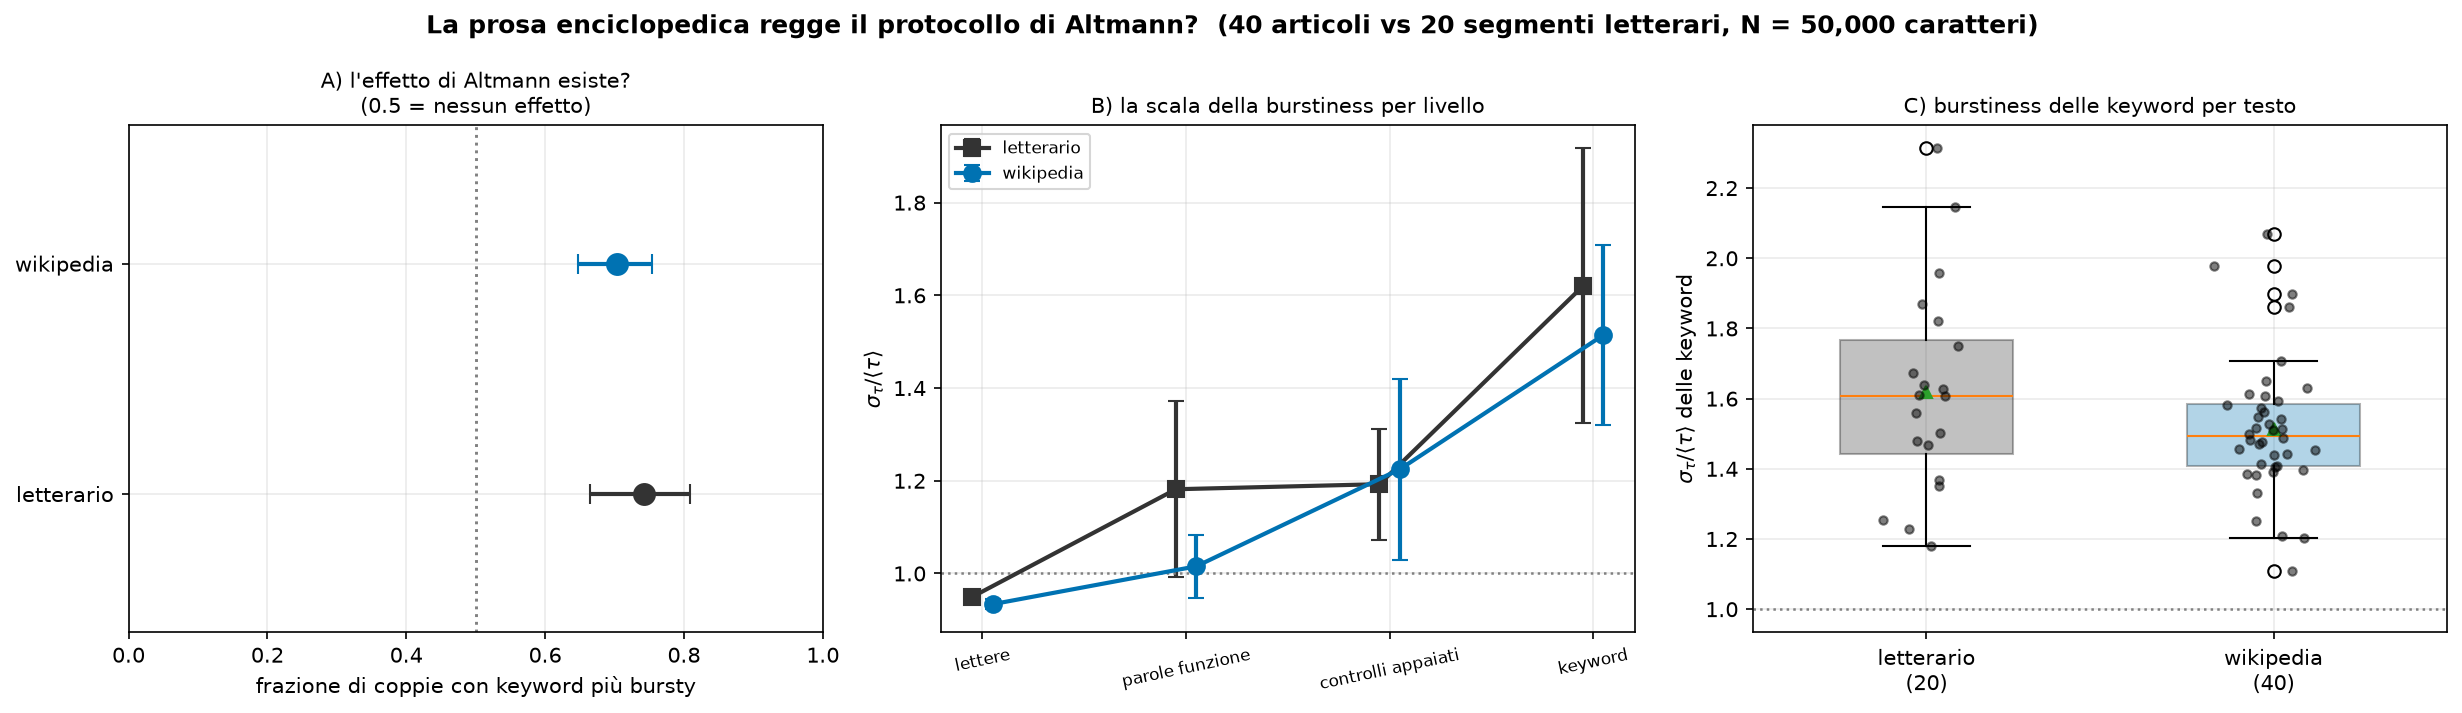
\includegraphics[width=\textwidth]{figure/cap5_wiki_altmann.png}
  \caption{Test di fattibilità del protocollo su prosa enciclopedica, condotto
  su \num{40} voci di Wikipedia e \num{20} segmenti letterari a \num{50000}
  caratteri. A: quota di confronti in cui la parola chiave supera il proprio
  controllo appaiato in frequenza, con intervallo di confidenza al $95\%$; la
  linea punteggiata a $0.5$ è l'assenza di effetto. B: coefficiente di
  variazione degli intervalli ai quattro livelli linguistici. C: distribuzione
  della burstiness delle parole chiave testo per testo. Questa è l'unica figura
  del capitolo costruita su \num{40} voci e \num{50000} caratteri; tutte le
  successive usano \num{39} terne e \num{60000} caratteri.}
  \label{fig:wiki-fattibilita}
\end{figure}

% ---------------------------------------------------------------------
\section{L'effetto nei tre corpora}
\label{sec:tre-corpora}

L'analisi principale confronta Wikipedia, le due versioni di Grokipedia e
l'ancora letteraria su \num{39} terne complete, troncate a \num{60000}
caratteri. La voce esclusa è \emph{Buddhism}, per la ragione riportata nel
§\ref{sec:paternita}: la sua versione v0.1 è ricopiata da Wikipedia, e in un
disegno appaiato un titolo che cade in un corpus deve cadere in tutti.

\paragraph{La finestra su cui l'esponente è stimato.}
L'esponente di correlazione $\hat\gamma$ è ottenuto interpolando
la~\eqref{eq:sigma} nell'intervallo fisso $t \in (100, 2000)$ caratteri.
\cite{altmann2012} adotta invece una regola relativa e ferma la finestra
all'uno per cento della lunghezza del testo. Le due scelte non sono ordinabili
una volta per tutte: applicata ai romanzi interi che quel lavoro analizza la
regola relativa dà un tetto dell'ordine di \num{10000} caratteri, molto più
largo di quello adottato qui; applicata alle finestre da \num{60000} caratteri
di questo capitolo dà $t < 600$, molto più stretto. L'intera catena è stata
ripetuta anche con la seconda. Il
livello medio di $\hat\gamma$ si abbassa di qualche centesimo, sulle parole
chiave da $1.23$ a $1.18$ per Wikipedia e da $1.32$ a $1.22$ per il romanzo,
ma l'ordinamento fra i corpora resta identico a tutti e quattro i livelli. Il
divario appaiato fra Grokipedia attuale e Wikipedia sulle parole chiave passa
da $-0.049$ a $-0.076$, cioè si accentua invece di ridursi, e resta
significativo in entrambi i casi. Le conclusioni di questo capitolo non
dipendono dunque dalla finestra scelta.

\paragraph{Tre modi di leggere il confronto.}
La Figura~\ref{fig:tre-corpora} riporta i tre modi in cui il confronto può
essere letto. Il primo pannello ripete il test del paragrafo precedente sui
quattro corpora: la quota di confronti vinti dalle parole chiave vale
$114/140 = 0.814$ sul romanzo, $189/273 = 0.692$ su Wikipedia,
$195/273 = 0.714$ su Grokipedia v0.1 e $202/273 = 0.740$ su Grokipedia nella
versione attuale. Ripetendo lo stesso test sull'esponente di correlazione
$\hat\gamma$ anziché sulla burstiness, la quota di confronti vinti dalle parole
chiave vale $0.907$ sul romanzo, $0.747$ su Wikipedia, $0.769$ su Grokipedia
v0.1 e $0.791$ su Grokipedia nella versione attuale.
L'effetto esiste ovunque, con tutti e quattro gli
intervalli di confidenza interamente sopra $0.5$, ed è massimo sul romanzo;
fra le due enciclopedie, però, non distingue: i valori di Grokipedia sono anzi
lievemente superiori a quelli di Wikipedia, con intervalli che si sovrappongono.
La domanda a cui questo pannello risponde è se la parola chiave superi il
proprio controllo a frequenza appaiata dentro lo stesso testo, e la
risposta è che ciò accade con la stessa frequenza nei due corpora enciclopedici.
Il deficit di Grokipedia, misurato dai pannelli successivi, non riguarda dunque
l'esistenza del meccanismo ma il livello assoluto della burstiness.

Il secondo pannello mostra il coefficiente di variazione ai quattro livelli e
rende visibile dove la differenza si concentra. Sulle lettere i quattro corpora
sono indistinguibili, tutti compresi fra $0.922$ e $0.950$, e sulle parole
funzione la separazione resta modesta, da $0.967$ a $1.192$. Il divario si apre
ai due livelli lessicali: sui controlli appaiati il romanzo raggiunge $1.262$,
Wikipedia $1.190$ e le due versioni di Grokipedia $1.044$ e $1.055$; sulle
parole chiave rispettivamente $1.789$, $1.536$, $1.387$ e $1.379$. 
Il terzo pannello riporta la stessa quantità testo per testo,
e mostra che la separazione non è l'effetto di pochi articoli anomali: le
distribuzioni di Wikipedia e di Grokipedia si sovrappongono, ma le loro mediane
differiscono di circa $0.25$ e la coda superiore di Wikipedia è più popolata.

\begin{figure}[htbp]
  \centering
  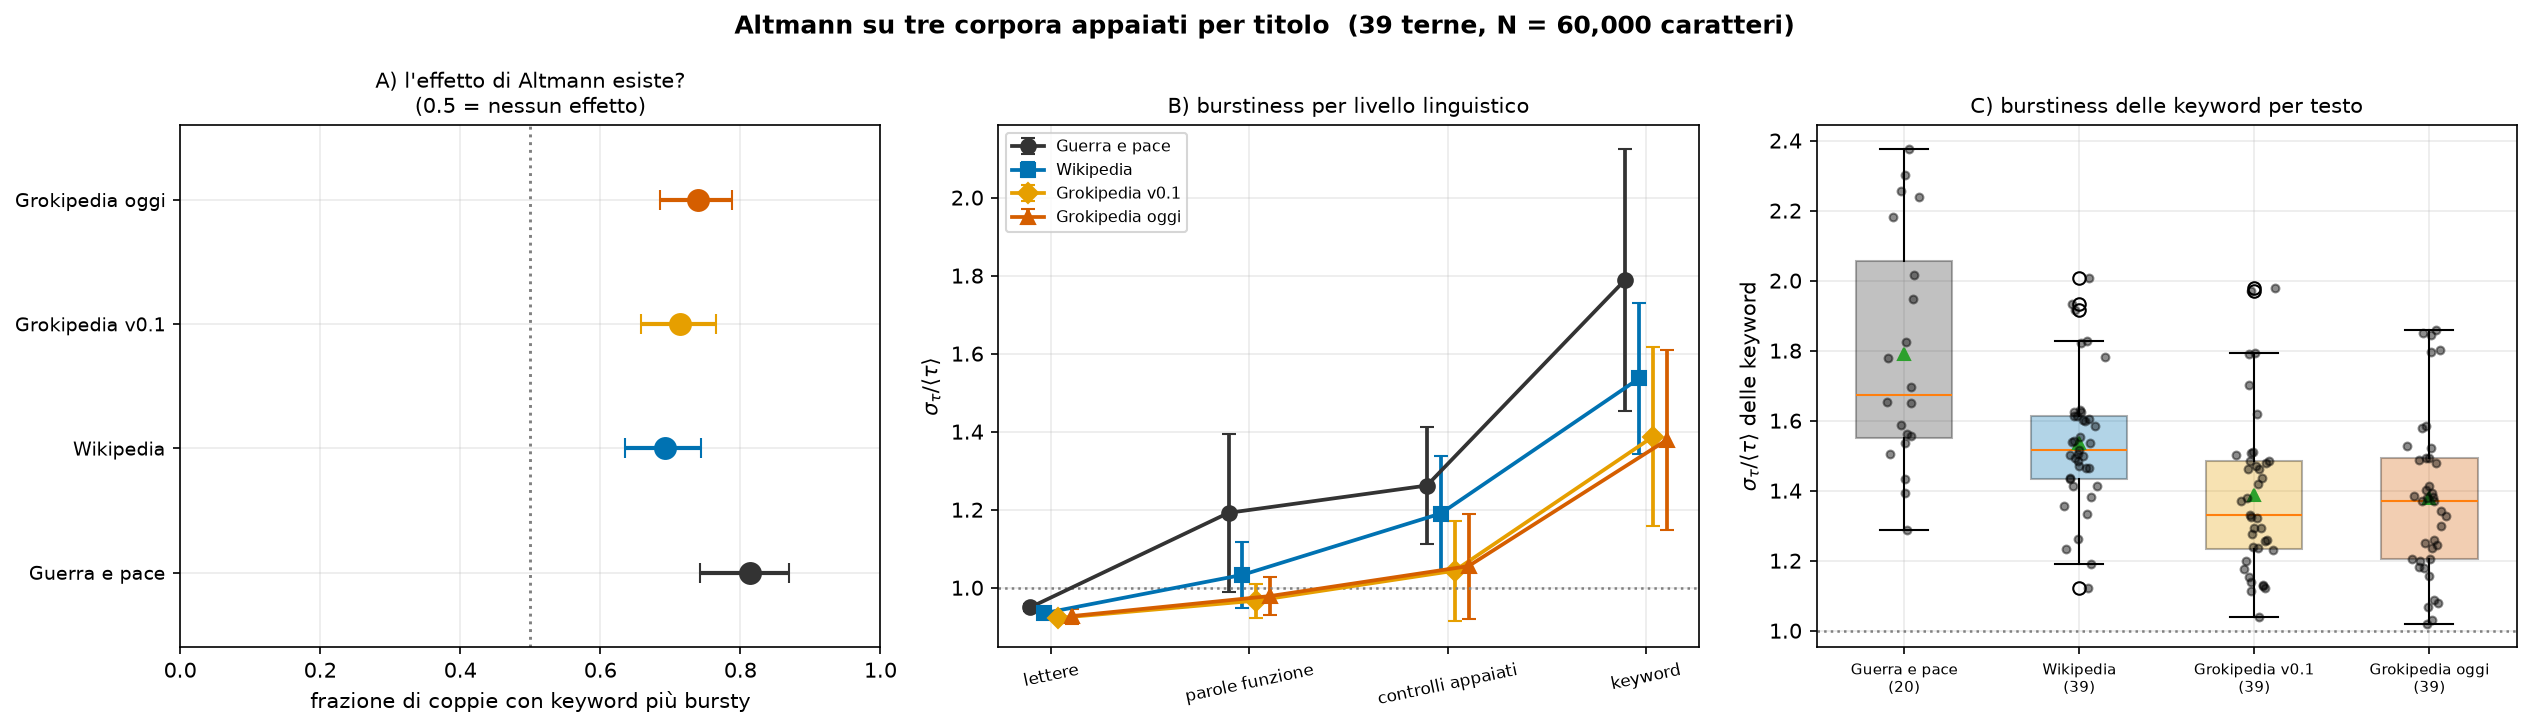
\includegraphics[width=\textwidth]{figure/cap5_tre_corpora.png}
  \caption{Il protocollo di Altmann sui quattro corpora, \num{39} terne
  appaiate per titolo a \num{60000} caratteri. A: quota di confronti vinti dalle
  parole chiave, con intervallo di confidenza al $95\%$. B: coefficiente di
  variazione degli intervalli ai quattro livelli linguistici; le barre sono
  deviazioni standard fra testi. C: burstiness delle parole chiave testo per
  testo, con mediana, quartili e singoli punti sovrapposti. Il numero di testi
  per corpus è indicato sotto ciascuna colonna.}
  \label{fig:tre-corpora}
\end{figure}

\paragraph{L'ancora letteraria è un testo, non un genere.} Il primato del
romanzo sui due livelli lessicali non sopravvive al cambio di testo. Ripetendo
l'intera misura su tre altri romanzi inglesi trattati esattamente come
\emph{Guerra e pace}, cioè \emph{Moby Dick}, \emph{Middlemarch} e \emph{David
Copperfield}, gli stessi impiegati come controllo nel
§\ref{sec:coda-risultati}, sulle parole chiave si ottiene $1.55$, $1.54$ e
$1.63$, cioè valori sostanzialmente pari a quello di Wikipedia e ben al di
sotto dell'$1.79$ di \emph{Guerra e pace}; alle parole funzione si ottiene
$1.03$, $1.08$ e $1.09$, contro l'$1.19$ del romanzo di riferimento e l'$1.03$
di Wikipedia. La distanza fra prosa letteraria e prosa enciclopedica non è
dunque un fatto generale, e l'ancora letteraria di questo capitolo va letta
per ciò che è: un termine di paragone concreto, non la misura di un genere.
Nulla di ciò che segue vi poggia, perché il risultato del capitolo è un
confronto appaiato fra le due enciclopedie, dove il romanzo non entra.

Il null model A1 restituisce un esponente medio di $0.983$ su tutte le celle,
in accordo con l'unità che deve dare per costruzione: la procedura di stima si
comporta come nel §\ref{sec:validazione} anche su questi corpora.

\paragraph{L'analogo della Figura~2 di~\cite{altmann2012}.}
La Figura~\ref{fig:altmann-fig2} riproduce sui quattro corpora la costruzione
con cui~\cite{altmann2012} presenta il proprio risultato principale, e permette
di verificarne l'aderenza riga per riga. Per ogni corpus vengono mostrate una
lettera e una parola di contenuto, ciascuna con la distribuzione cumulata degli
intervalli e con la crescita della varianza del conteggio, accanto alle stesse
curve calcolate sui due null model.

\paragraph{Quale parola mostrare.} La scelta della parola da mostrare pone un
problema che il caso della lettera non ha. Selezionare la parola chiave più
ricorrente del corpus, che è il criterio più immediato, produce oggetti
strutturalmente diversi nei due tipi di prosa: in un romanzo pesca il nome di
un personaggio, presente solo nelle scene in cui il personaggio compare,
mentre in un'enciclopedia pesca il soggetto della voce, che ricorre in quasi
ogni frase. Le due parole finirebbero alle code opposte delle rispettive
distribuzioni di burstiness, al $96$ e al $2$ percentile, e la figura
confronterebbe due casi estremi anziché due casi tipici. La parola mostrata è
quindi quella con $\sigma_\tau/\langle\tau\rangle$ più vicino alla mediana del
proprio corpus, fra quelle con almeno \num{40} occorrenze; il percentile
effettivo è riportato sopra ciascun pannello e sta fra $45$ e $57$ in tutti e
quattro i corpora. Il caso escluso ha però un interesse proprio, ed è ripreso
subito dopo la figura.

\paragraph{Che cosa mostrano le quattro righe.}
Il comportamento è allora quello descritto nel §\ref{sec:origini}, e vale su
tutte e quattro le righe. Sulla lettera la cumulata decade rapidamente e
l'esponente del null model A2 si dispone attorno all'unità, $0.94$ sul romanzo,
$0.90$ su Wikipedia, $0.94$ sulla v0.1 e $1.05$ sulla versione attuale di
Grokipedia, perché a quel livello la burstiness non contribuisce. Lo scarto
massimo da uno vale un decimo, ed è quanto ci si attende su una singola
sequenza: aggregando tutte le \num{2603} sequenze di livello letterale dei
quattro corpora $\hat\gamma_{A2}$ vale fra $0.983$ e $0.990$, con una
dispersione fra sequenze di $0.044$, cosicché i quattro valori della figura
stanno tutti entro due deviazioni standard dall'unità. Un solo caso per corpus
non permette dunque una lettura più fine di così.

Sulla parola di contenuto la cumulata ha coda larga, con
$\sigma_\tau/\langle\tau\rangle$ fra $1.23$ e $1.79$, e $\hat\gamma_{A2}$
resta sopra l'unità e più vicino a $\hat\gamma$ che nel caso della lettera:
$1.36$ contro $1.43$ sul romanzo, $1.09$ contro $1.20$ su Wikipedia, $1.09$
contro $1.23$ sulla v0.1 e $1.11$ contro $1.20$ sulla versione attuale. Una
parte della correlazione passa cioè attraverso la distribuzione degli
intervalli, e la frazione è massima sul romanzo. La figura mostra il
meccanismo su un caso per corpus e non va letta come misura del divario fra
corpora: quella richiede l'aggregato del §\ref{sec:decomposizione}, perché su
una singola parola la differenza fra i due esponenti è dominata dal rumore di
stima. Lo si vede nella riga di Grokipedia attuale, dove sulla lettera
$\hat\gamma = 0.94$ scende sotto $\hat\gamma_{A2} = 1.05$, cosa che
sull'aggregato di quel livello, dove il rumore si media, non accade.

La lettera \emph{e} in \emph{Guerra e pace} dà qui un coefficiente di
variazione pari a $0.85$ contro lo $0.83$ della didascalia della Figura~2
di~\cite{altmann2012}, il che vale come controllo indipendente delle
procedure: la stessa quantità, misurata sullo stesso testo da un codice
diverso, coincide entro due centesimi.

\begin{figure}[htbp]
  \centering
  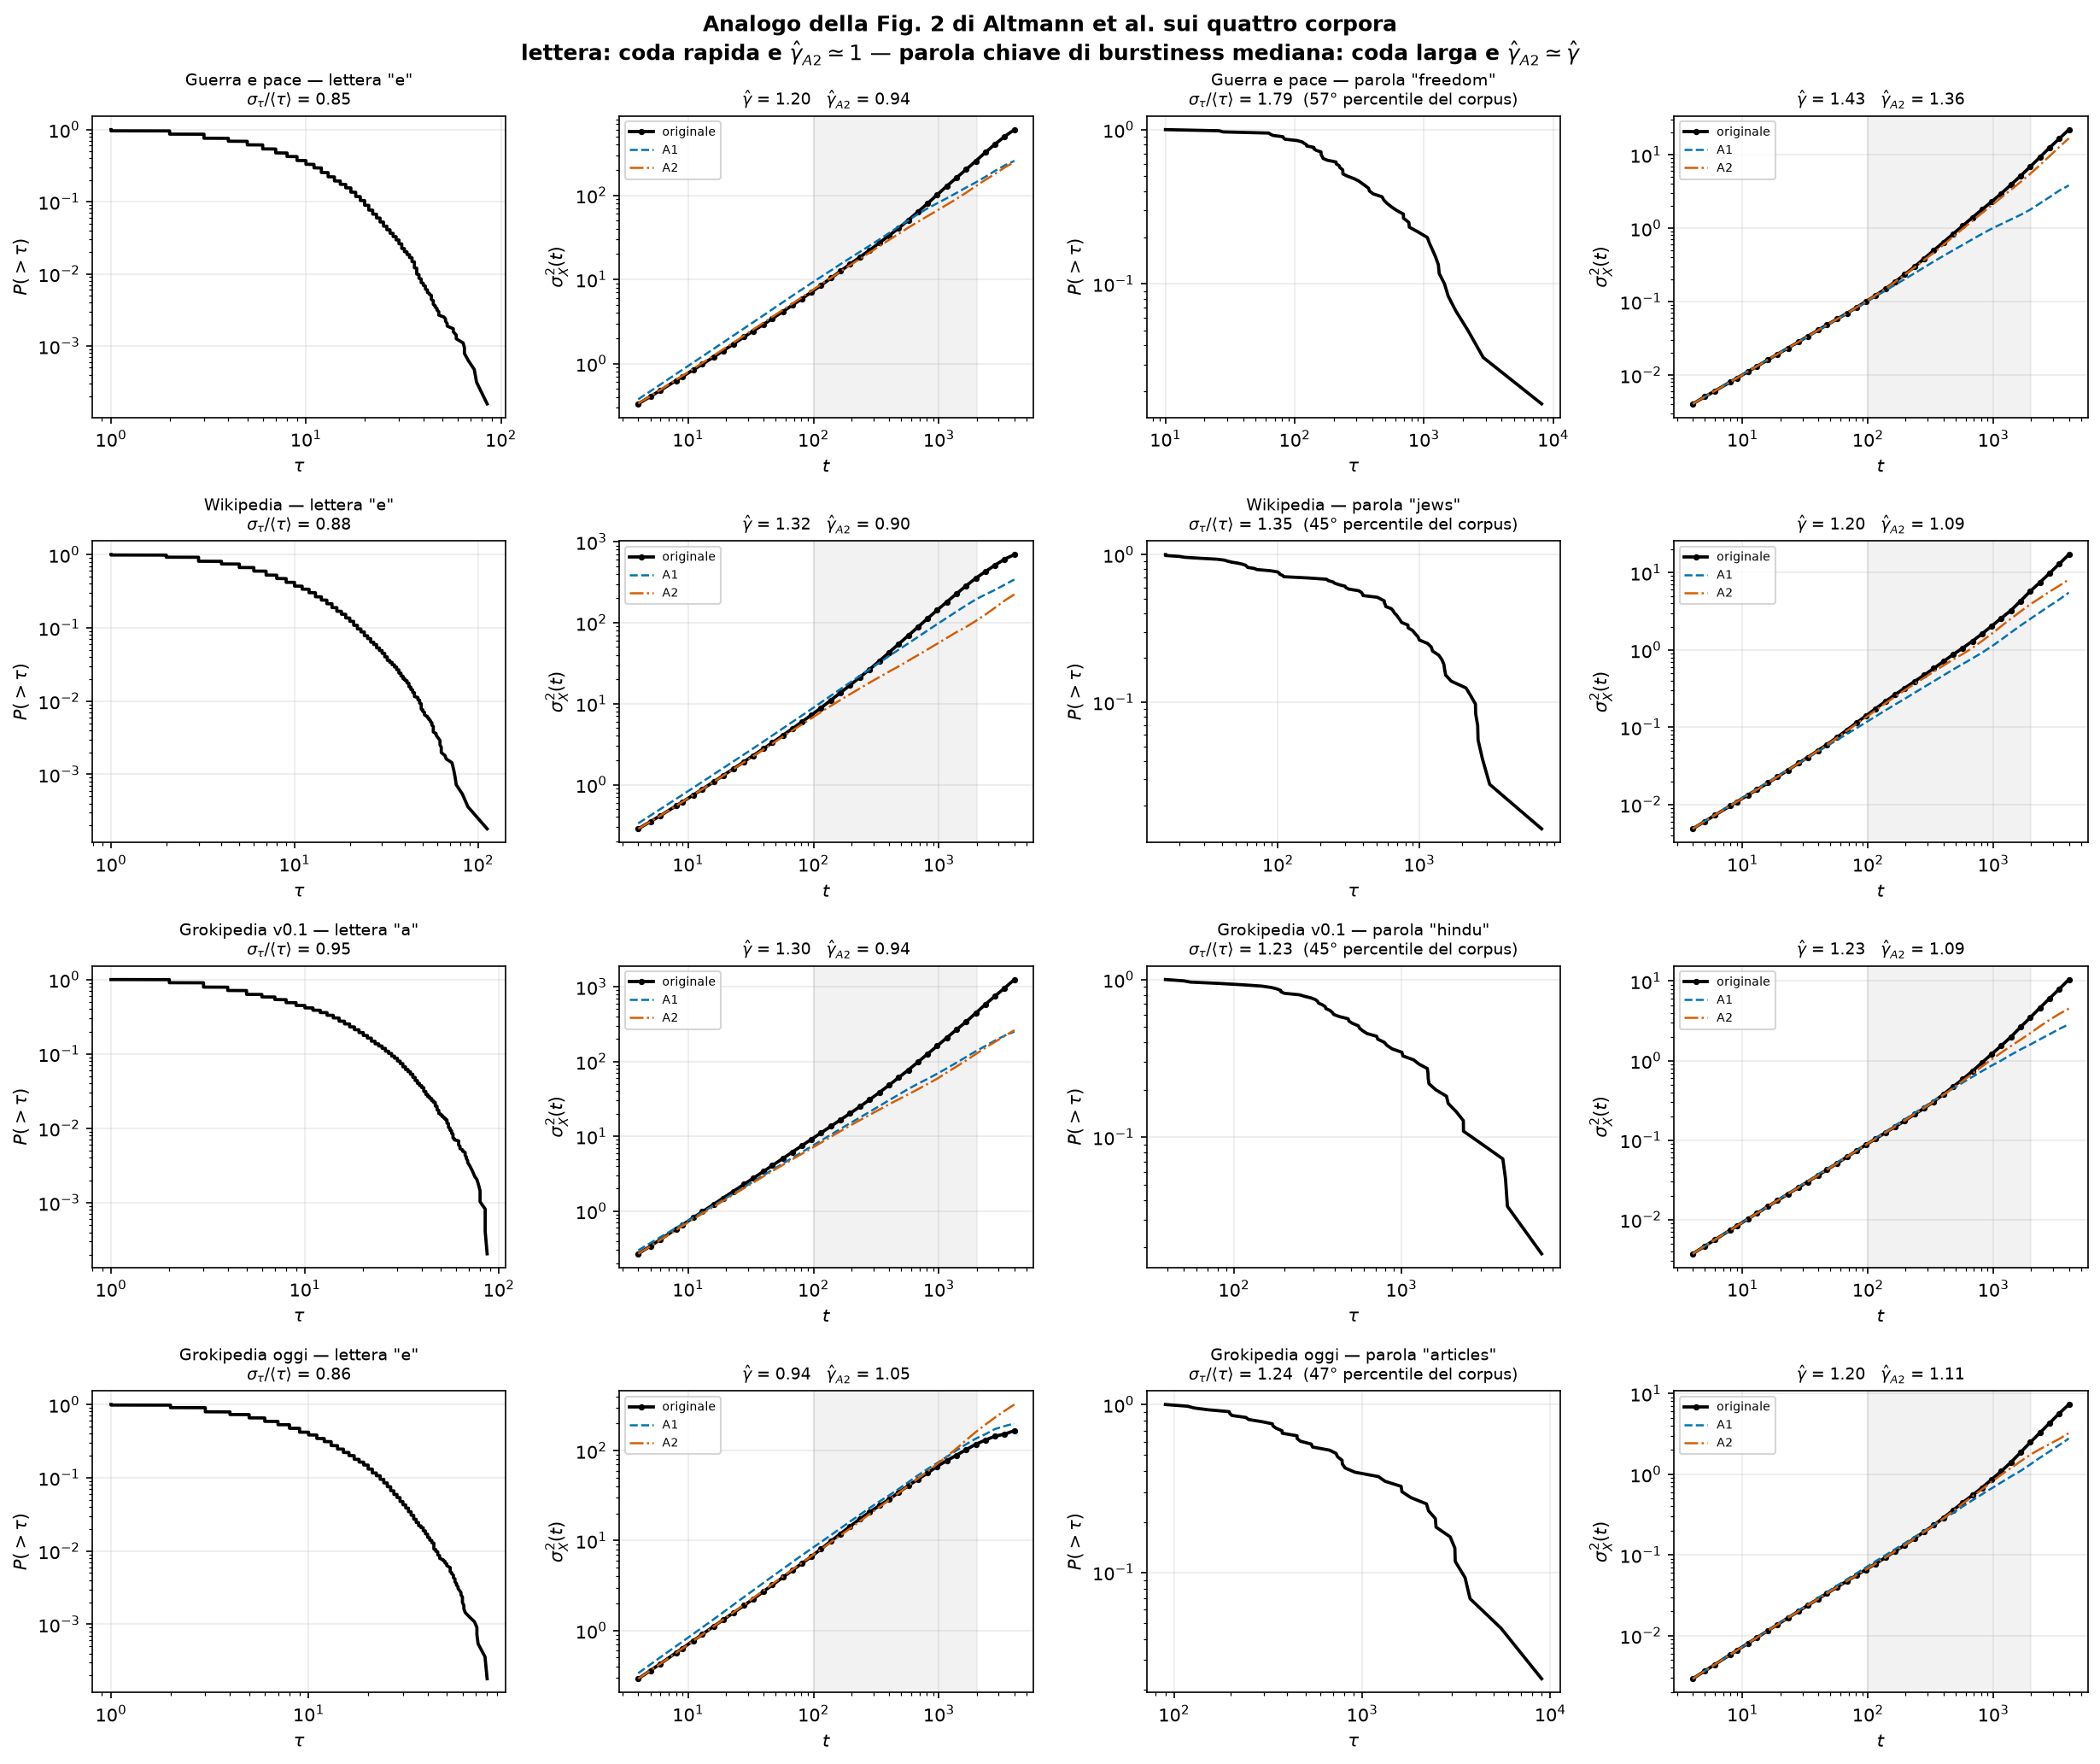
\includegraphics[width=\textwidth]{figure/cap5_altmann_fig2.png}
  \caption{Analogo della Figura~2 di~\cite{altmann2012} sui quattro corpora. Una
  riga per corpus; a sinistra la lettera più frequente del documento, a destra
  la parola chiave di burstiness mediana del corpus fra quelle con almeno
  \num{40} occorrenze, con il suo percentile indicato sopra il pannello. Per
  ciascuna, la distribuzione cumulata degli intervalli $P(>\tau)$ e la crescita
  della varianza del conteggio $\sigma_X^2(t)$, con le curve dei due null model
  del §\ref{sec:null} e la finestra di fit ombreggiata. La lettera ha coda
  rapida e $\hat\gamma_{A2} \simeq 1$; la parola di contenuto ha coda larga e
  $\hat\gamma_{A2}$ prossimo a $\hat\gamma$.}
  \label{fig:altmann-fig2}
\end{figure}

\paragraph{Il soggetto della voce non è una parola di contenuto.}
La parola chiave più ricorrente di un articolo enciclopedico, quella che il
criterio scartato sopra avrebbe selezionato, si comporta in modo opposto a
quello che il §\ref{sec:origini} prevede per il suo livello linguistico. Nella
voce \emph{Alexander the Great} di Wikipedia la parola \emph{alexander} ha
$\sigma_\tau/\langle\tau\rangle = 0.78$; in \emph{Sigmund Freud} di Grokipedia
\emph{freud} ha $0.72$. Sono valori sotto il limite poissoniano, cioè
distribuzioni \emph{più regolari del caso}, mentre la lettera \emph{e} negli
stessi testi dà $0.84$. Il confronto con la lettera non va però fatto sul valore
grezzo. Per un processo casuale in tempo discreto
$\sigma_\tau/\langle\tau\rangle$ non vale esattamente uno, ma tanto meno quanto
più corti sono gli intervalli: il null model A1, applicato alla stessa frequenza
della sequenza osservata, restituisce $0.95$ per la lettera \emph{e}, che ricorre
ogni dieci caratteri, e $1.00$ per una parola chiave, che ricorre ogni
duecento.

\paragraph{Il riferimento casuale dipende dalla frequenza.}
La ragione di quel $0.95$ è che gli intervalli sono numeri interi positivi. Se
le occorrenze sono collocate a caso con probabilità $f$ per carattere, la
distanza fra due consecutive è geometrica, e per la geometrica si ha
$\sigma_\tau/\langle\tau\rangle = \sqrt{1-f}$: il valore tende a uno solo nel
limite di eventi rari. Con $f = 1/10$, la frequenza della lettera \emph{e}, si
ottiene $0.949$; con $f = 1/200$, la frequenza tipica di una parola chiave,
$0.997$. Il valore poissoniano di riferimento non è dunque lo stesso ai due
livelli, ed è più basso proprio dove gli eventi sono più fitti. Confrontare
\emph{alexander} e la lettera \emph{e} sui valori grezzi significherebbe
attribuire alla struttura del testo una differenza che è invece un effetto
della sola frequenza.

Rapportando ciascuna misura al proprio valore casuale l'effetto si toglie, e
resta $0.78$ per \emph{alexander} contro $0.88$ per la lettera: il soggetto
della voce è più regolare di una lettera anche dopo aver tolto l'effetto della
frequenza, e la differenza fra i due, lungi dall'essere prodotta dalla
normalizzazione, ne esce accentuata.

\paragraph{Perché il soggetto si comporta così.}
La ragione è che in prosa enciclopedica il soggetto non è un tema fra altri,
che alterna presenza e assenza lungo il testo, ma il tema unico: compare come soggetto grammaticale di quasi ogni
periodo, e i suoi intervalli ereditano allora la statistica della lunghezza
delle frasi anziché quella dell'alternanza tematica. La verifica è diretta.
Nei sei articoli esaminati il soggetto ricorre una volta ogni $1.4$--$1.7$
frasi, con lo stesso valore in Wikipedia e in Grokipedia. I suoi intervalli sono
quindi lunghezze di frase, e ne ereditano la variabilità: le
lunghezze di frase di quegli articoli hanno
$\sigma_\tau/\langle\tau\rangle$ fra $0.33$ e $0.73$, e il soggetto della voce
si colloca poco sopra, fra $0.54$ e $0.78$, comunque sotto l'unità che
segnerebbe l'assenza di struttura. Per confronto, \emph{natásha} in un segmento
di \emph{Guerra e pace} ricorre una volta ogni $5.1$ frasi e ha
$\sigma_\tau/\langle\tau\rangle = 3.24$: lì la ricorrenza non segue il ritmo del
periodo ma l'alternanza delle scene.

Il soggetto della voce funziona quindi da marcatore sintattico e non semantico,
e la sua ricorrenza è governata dal ritmo del periodo, non dalla persistenza di
un argomento. Non è un difetto della misura ma un tratto del genere
enciclopedico, e va tenuto presente nel confrontare la burstiness lessicale fra
generi diversi: è la ragione per cui la parola mostrata nella
Figura~\ref{fig:altmann-fig2} viene scelta sulla mediana e non sul massimo.

% ---------------------------------------------------------------------
\section{Il divario si apre al livello lessicale}
\label{sec:appaiato}

L'appaiamento per titolo permette un test più stringente del confronto fra
medie. Confrontare la media di Wikipedia con quella di Grokipedia lascia
aperta l'obiezione che le due medie siano calcolate su argomenti diversi, e
che la differenza rifletta il contenuto anziché la scrittura. Il test appaiato
la chiude: per ciascuna delle \num{39} voci, che nei due corpora tratta lo
stesso argomento, si calcola la differenza fra il valore di Grokipedia e
quello di Wikipedia, e si verifica con il test dei ranghi segnati di Wilcoxon
che la mediana di quelle \num{39} differenze sia diversa da zero. Il test è
non parametrico, quindi non assume che le differenze siano distribuite
normalmente, assunzione che con \num{39} osservazioni e distribuzioni
asimmetriche non sarebbe difendibile.

Il test dà, per la versione attuale di Grokipedia,
$-0.167$ sulle parole chiave e $-0.010$ sulle lettere; ai due livelli intermedi
le differenze valgono $-0.037$ per le parole funzione e $-0.157$ per i controlli
appaiati, tutte con significatività inferiore a $10^{-2}$. La versione v0.1 dà
$-0.012$, $-0.039$, $-0.116$ e $-0.133$.

I quattro numeri vanno letti come una scala. Alle lettere Grokipedia e
Wikipedia distano un centesimo di unità di burstiness, cioè circa l'uno per
cento del valore misurato: a quel livello i due corpora sono, in pratica, lo
stesso testo. Alle parole funzione la distanza quadruplica, ma resta piccola in
termini relativi. Ai due livelli lessicali passa a circa sedici centesimi, oltre
un decimo del valore misurato e più di un ordine di grandezza sopra il livello
delle lettere.

La scala ha però un solo gradino, non tre. La differenza fra i livelli
sub-lessicali e quelli lessicali è netta; quella fra i due livelli lessicali non
esiste: $-0.157$ sui controlli a frequenza appaiata contro $-0.167$ sulle parole
chiave sono lo stesso numero. Il testo generato non perde dunque le parole di
contenuto più di quanto perda le altre parole della stessa frequenza. Ciò che i
dati sostengono è che riproduca le regolarità dei livelli bassi e abbassi
uniformemente la burstiness a livello di parola, non che perda selettivamente la
persistenza tematica.

\paragraph{Il divario alla lunghezza di controllo.}
\label{sec:robustezza-neff}
L'intera catena è stata ripetuta a $N_{\mathrm{eff}} = \num{80000}$ caratteri,
lunghezza a cui sopravvivono \num{35} delle \num{39} terne; per isolare
l'effetto della finestra, i valori a \num{60000} sono ricalcolati sulle stesse
\num{35}. Alle lettere e alle parole funzione il divario appaiato è stabile, da
$-0.010$ a $-0.011$ e da $-0.037$ a $-0.045$; ai due livelli lessicali si separa
in direzioni opposte, con i controlli appaiati da $-0.164$ a $-0.195$ e le parole
chiave da $-0.167$ a $-0.130$, quest'ultima con significatività che scende a
$p = 0.027$. Alla lunghezza maggiore il divario sulle parole chiave è dunque
\emph{minore} di quello sui controlli appaiati. Ciò che risulta robusto è il
salto dal livello sub-lessicale a quello lessicale; l'ulteriore crescita fino
alle parole chiave non lo è. Anche l'esponente di coda è instabile fra le due
lunghezze, da $2.19$ a $2.50$ su Grokipedia e da $2.37$ a $2.25$ su Wikipedia,
coerentemente con l'avvertenza del §\ref{sec:coda-risultati}.

La Figura~\ref{fig:altmann-fig3} riporta le stesse sequenze nel piano che
\cite{altmann2012} usa per la propria Figura~3: la burstiness in ascissa e
l'esponente di correlazione in ordinata, un punto per sequenza, con un simbolo
diverso per livello linguistico. La gerarchia vi si legge come una disposizione
spaziale: le lettere, gli spazi e le vocali si addensano in una colonna stretta
attorno a $\sigma_\tau/\langle\tau\rangle \simeq 0.5$, le parole funzione e i
controlli appaiati occupano la regione centrale, le parole chiave si spingono a
destra e in alto. È la stessa gerarchia dei paragrafi precedenti, vista tutta
insieme invece che un livello alla volta.

Il piano rende però visibile anche una proprietà che i confronti per livello
non mostrano, e che è l'osservazione centrale di quel lavoro: l'angolo in
basso a destra è vuoto. Non esistono, cioè, sequenze molto \emph{bursty} e
insieme poco correlate. Sui quattro corpora di questa tesi la regolarità si
quantifica così: delle $451$ sequenze con $\sigma_\tau/\langle\tau\rangle >
1.5$, soltanto $17$, il $3.8\%$, hanno $\hat\gamma < 1.1$, e fra quelle con
burstiness superiore a $2$ l'esponente non scende mai sotto $1.05$. L'angolo
opposto, invece, è popolato: delle $3500$ sequenze sotto il valore poissoniano
$\sigma_\tau/\langle\tau\rangle = 1$, il $15.9\%$ ha $\hat\gamma > 1.2$.

L'asimmetria fra i due angoli è la firma di una relazione a senso unico. La
burstiness produce correlazione, come mostra la~\eqref{eq:eq4}, e una sequenza
con vuoti lunghi non può quindi risultare scorrelata; il viceversa non vale,
perché la correlazione può venire anche dall'ordine degli intervalli e
manifestarsi senza alcuna coda pesante. La correlazione di rango fra le due
quantità è positiva e significativa in tutti e quattro i corpora, da $+0.22$ su
Wikipedia a $+0.36$ sul romanzo. Il meccanismo descritto in~\cite{altmann2012}
sui romanzi si ritrova dunque identico nella prosa enciclopedica e in quella
generata, ed è un risultato indipendente dal divario misurato sopra: riguarda
come le due grandezze si legano fra loro, non quanto valgano.

\begin{figure}[htbp]
  \centering
  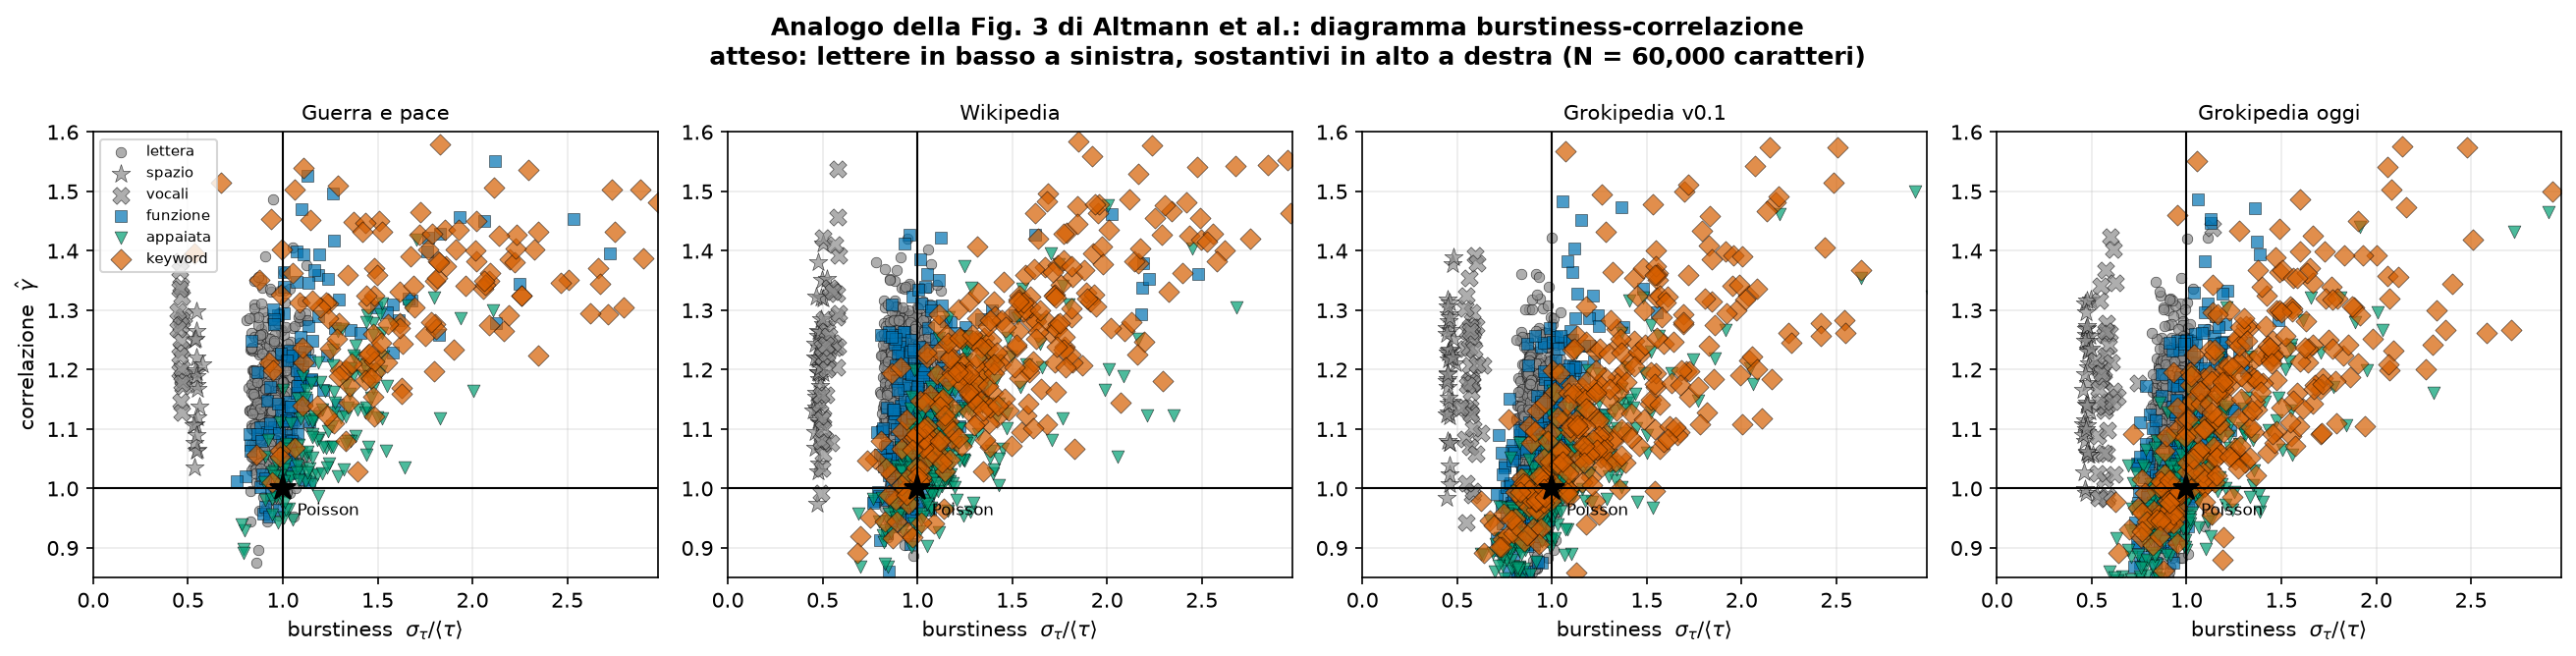
\includegraphics[width=\textwidth]{figure/cap5_altmann_fig3.png}
  \caption{Analogo della Figura~3 di~\cite{altmann2012}: diagramma
  burstiness--correlazione sui quattro corpora, un punto per sequenza. Oltre ai
  quattro livelli usati nel resto del capitolo sono riportati i due livelli
  sub-lessicali tenuti come diagnostica, gli spazi e le vocali. Le linee nere
  segnano il processo di Poisson,
  $\sigma_\tau/\langle\tau\rangle = 1$ e $\hat\gamma = 1$. L'angolo in basso a
  destra è praticamente vuoto in tutti e quattro i corpora: sequenze molto
  bursty e insieme poco correlate non si osservano.}
  \label{fig:altmann-fig3}
\end{figure}

\paragraph{I due quadranti che restano.} La lettura del piano fatta finora
riguarda la diagonale: l'angolo in basso a destra vuoto e quello in alto a
sinistra popolato. Gli altri due separano però i corpora meglio di qualunque
media, e la Figura~\ref{fig:quadranti} li riporta separatamente. Fra le parole
chiave, l'angolo in alto a destra è la posizione canonica
di~\cite{altmann2012}, quella in cui la sequenza è insieme bursty e correlata.
Vi ricade il $91.4\%$ delle sequenze di \emph{Guerra e pace} e l'$87.5\%$ di
quelle di Wikipedia, ma solo il $74.0\%$ di Grokipedia v0.1 e il $77.3\%$
della versione attuale. La differenza finisce quasi interamente nell'angolo
opposto, in basso a sinistra, dove la parola è più regolare di un processo di
Poisson e insieme priva di correlazione a lungo raggio: $0\%$ sul romanzo,
$5.1\%$ su Wikipedia, $15.4\%$ su Grokipedia v0.1 e $14.3\%$ sulla versione
attuale. Una parola chiave generata su sette si trova dunque nell'angolo
opposto a quello canonico, contro una su venti in Wikipedia. Il test appaiato
sulle \num{39} voci conferma che non è un effetto di composizione del
campione: la quota di parole chiave in basso a sinistra cresce in $21$ e $22$
voci su $39$, con differenza mediana $+0.143$ e $p < 10^{-3}$ per entrambe le
versioni.

Due controlli escludono le spiegazioni strumentali. Il null model A1
restituisce $\hat\gamma = 0.983$ in tutti e quattro i corpora, identico alla
terza cifra, quindi la soglia $\hat\gamma = 1$ non è tarata diversamente da un
corpus all'altro; il valore calibrato non è però esattamente uno, cosicché la
soglia è lievemente generosa verso il lato correlato, allo stesso modo per
tutti. E la quota di parole in basso a sinistra resta più alta in Grokipedia
dentro quattro fasce di frequenza su cinque, da $0.159$ contro $0.050$ per le
parole con $26$--$35$ occorrenze a $0.303$ contro $0.076$ per quelle con più di
$80$. Fa eccezione la fascia più bassa, $15$--$25$ occorrenze, dove il rapporto
si inverte, $0.065$ contro $0.200$; lì però le parole chiave di Wikipedia sono
dieci in tutto e la quota è stimata su di esse. Il divario non dipende quindi
dal fatto che le parole chiave di Wikipedia siano più frequenti, salvo nella
fascia in cui il confronto ha meno appoggio.

Guardare dentro il quadrante non rivela più un gruppo omogeneo. Separando le
parole che compaiono nel titolo della voce dalle altre, le $14$ di Wikipedia si
dividono a metà, e le $39$ di Grokipedia si dividono in $18$ soggetti di voce e
$21$ altre parole, prevalentemente aggettivi generici: \emph{economic} in cinque
voci, \emph{military} in tre, \emph{urban} in due. Sono concentrazioni modeste,
e soprattutto non sono più quelle che la lista di parole funzione originaria
lasciava passare: con quella lista, il quadrante conteneva \emph{like} in dodici
voci, \emph{amid} in nove e \emph{including} in sei, cioè i connettivi che
costituiscono il vizio stilistico più evidente del testo generato. Quei termini
sono ora classificati come parole funzione, che è ciò che sono, e il
§\ref{sec:effetto-stoplist} misura quanto la loro presenza fra le parole chiave
alterasse i risultati.

\begin{figure}[htbp]
  \centering
  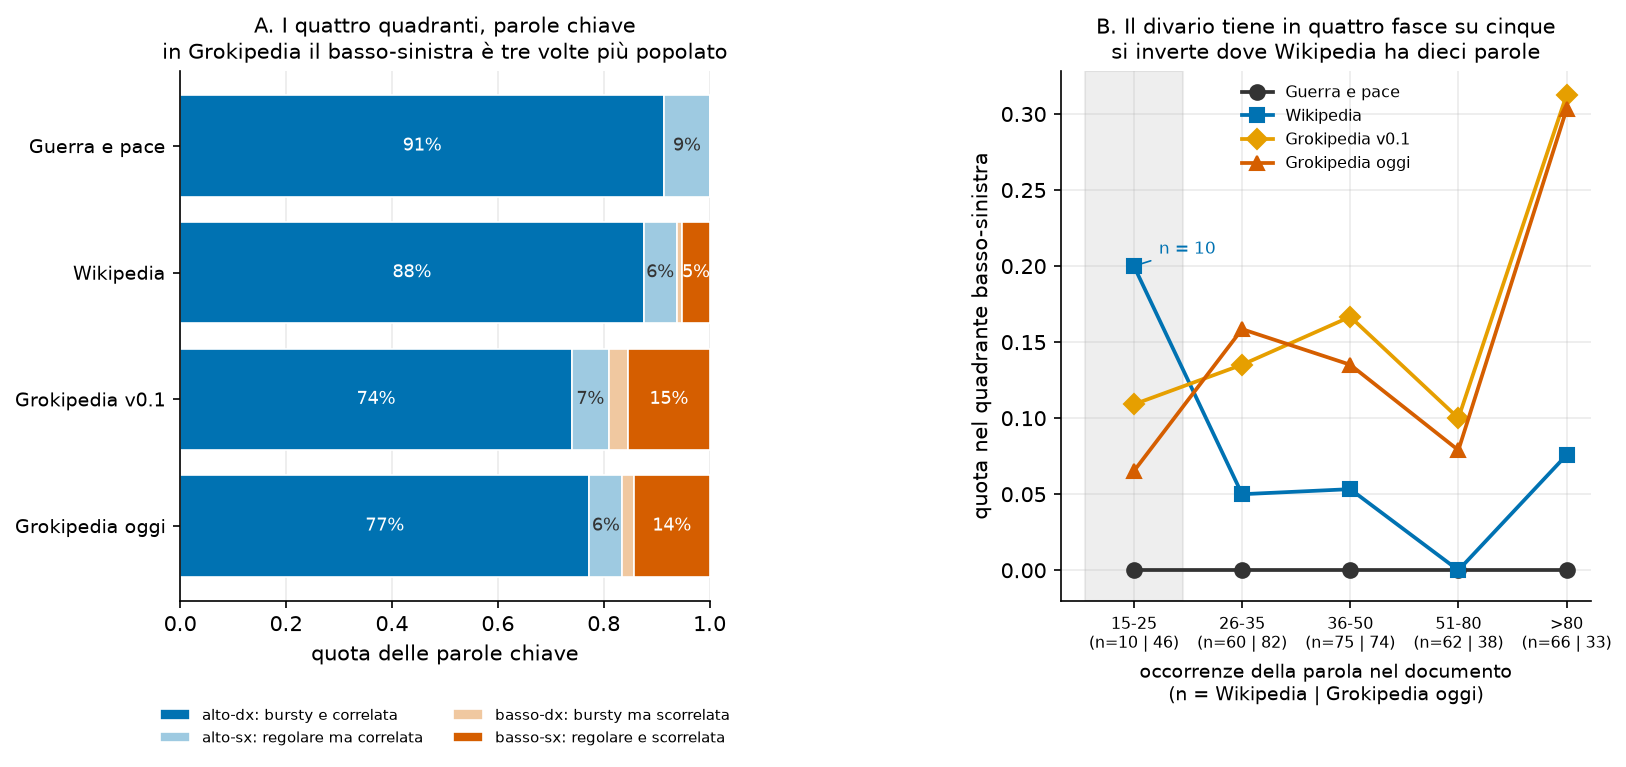
\includegraphics[width=\textwidth]{figure/cap5_quadranti.png}
  \caption{Lettura per quadranti del piano della
  Figura~\ref{fig:altmann-fig3}, sulle sole parole chiave. A: composizione per
  quadrante, un corpus per riga; le quote sotto il $5\%$ non sono etichettate. B:
  quota di parole chiave nel quadrante in basso a sinistra, separando le parole
  per numero di occorrenze nel documento; sotto ciascuna fascia è indicato
  quante parole chiave vi cadono in Wikipedia e in Grokipedia. Il divario tiene
  in quattro fasce su cinque e si inverte nella più bassa, dove Wikipedia ne ha
  dieci in tutto e la fascia è ombreggiata per segnalarlo.}
  \label{fig:quadranti}
\end{figure}

\paragraph{Un effetto di scala da neutralizzare.} Le voci di Grokipedia hanno
frasi sensibilmente
più lunghe di quelle di Wikipedia: $4.38$ frasi ogni mille caratteri contro
$6.92$. Poiché in questo capitolo il tempo è contato in caratteri, la scala
degli intervalli $\tau$ non è la stessa nei due corpora, e un testo con frasi
più lunghe tende ad avere intervalli più lunghi anche a parità di struttura
tematica. Il coefficiente di variazione è un rapporto e non risente di una
dilatazione uniforme dell'asse, ma la dilatazione qui non è uniforme, perché
agisce solo sui livelli definiti su unità linguistiche. Il
§\ref{sec:entropia-intervalli} introduce la misura che elimina il problema;
fino a quel punto il divario va considerato provvisorio.

Il riferimento letterario, infine, non è appaiato per argomento con nessuno dei
tre corpora enciclopedici: entra nei confronti come livello medio e non nei test
appaiati.

% ---------------------------------------------------------------------
\section{Quale meccanismo genera la correlazione}
\label{sec:decomposizione}

Sapere che un testo ha correlazioni a lungo raggio non dice da dove esse
vengano. Il §\ref{sec:null} ha introdotto i due null model che separano le due
origini possibili e la quota di burstiness $q$ della~\eqref{eq:quota}, che vale
circa uno quando la correlazione è interamente spiegata dalla distribuzione
degli intervalli, e circa zero quando è invece l'ordine in cui le occorrenze si
susseguono a produrla.

Il primo pannello della Figura~\ref{fig:decomposizione} riporta $q$ ai quattro
livelli. Sulle lettere il valore è negativo in tutti e quattro i corpora, da
$-0.06$ su Wikipedia a $-0.19$ su Grokipedia v0.1: le lettere sono correlate,
come mostra il $\hat\gamma$ maggiore di uno, ma non sono \emph{bursty}, e la
correlazione viene interamente dall'ordine. Sulle parole chiave il valore sale a
$0.89$ sul romanzo, $0.77$ su Wikipedia, $0.70$ sulla v0.1 e $0.74$ sulla
versione attuale di Grokipedia: qui quasi tutta la correlazione è già contenuta nella
distribuzione degli intervalli. I due livelli intermedi interpolano fra i due
regimi in modo ordinato.

La dissociazione fra il livello dei caratteri e quello del contenuto, che
in~\cite{altmann2012} è osservata su romanzi, si ritrova quindi identica nella
prosa enciclopedica e anche nella prosa generata. Il secondo pannello mostra la
stessa cosa in termini di esponenti: le curve piene sono $\hat\gamma$ e quelle
tratteggiate $\hat\gamma_{A2}$, e la distanza verticale fra le due è il
contributo dell'ordine delle occorrenze. Sulle lettere le due curve sono
separate e la tratteggiata sta all'unità; sulle parole chiave si avvicinano e
salgono insieme.

I valori dei tre corpora enciclopedici sono però troppo vicini perché la
differenza sia interpretabile: fra Wikipedia e Grokipedia vale $0.03$ alla
lunghezza di lavoro e cambia segno a quella di controllo del
§\ref{sec:robustezza-neff}. I dati non consentono quindi di attribuire ai due
corpora un'origine diversa della correlazione, ma soltanto un'intensità diversa.

Sulla riga dei controlli appaiati per Grokipedia, infine, la quota è stimabile
solo su $6$ documenti su $39$ per la versione v0.1 e su $8$ per quella
attuale. La ragione non è un difetto della stima ma la grandezza stessa: $q$
ha $\hat\gamma - 1$ al denominatore, e viene calcolata soltanto dove quel
denominatore supera $0.05$, perché sotto quella soglia il rapporto è dominato
dall'errore. A quel livello i documenti di Grokipedia hanno $\hat\gamma$
mediano pari a $1.003$ per la v0.1 e $1.015$ per la versione attuale, contro
$1.091$ di Wikipedia: le loro sequenze di controllo sono essenzialmente
scorrelate, e non c'è alcuna correlazione da decomporre nelle due origini.
L'esclusione è quindi essa stessa un dato, perché è il livello in cui il testo
generato si avvicina di più al caso, ma il valore di $q$ che sopravvive sui
pochi documenti restanti riguarda proprio quelli in cui una correlazione c'è,
e non va letto come una misura del corpus.

\begin{figure}[htbp]
  \centering
  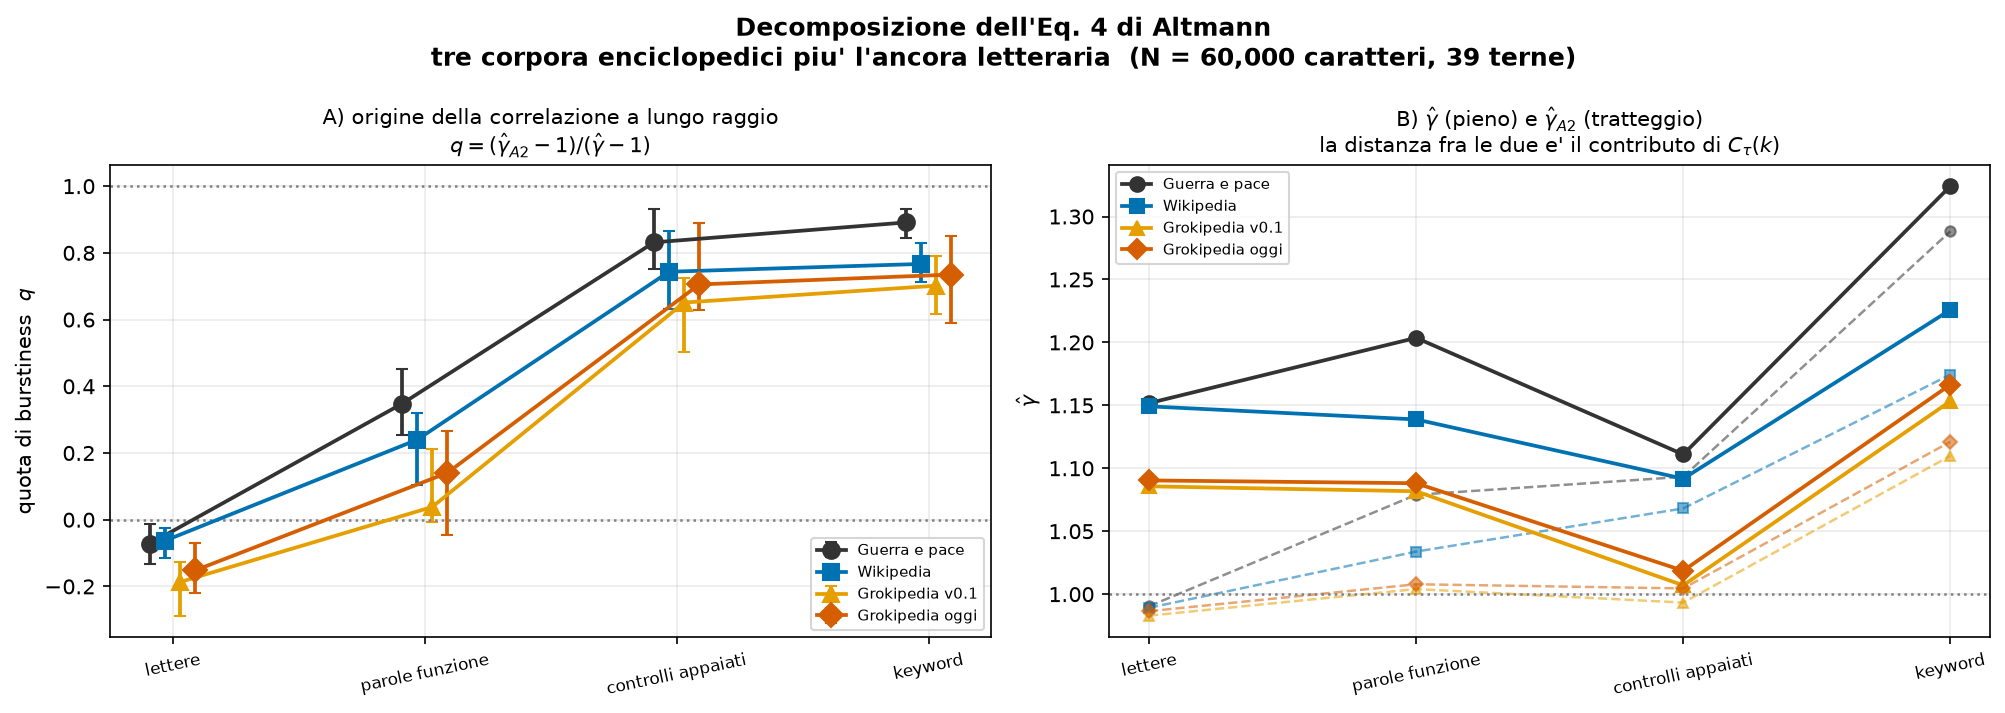
\includegraphics[width=\textwidth]{figure/cap5_decomposizione_eq4.png}
  \caption{Decomposizione della correlazione nelle sue due origini. A: quota
  $q$ della~\eqref{eq:quota} ai quattro livelli linguistici, con intervalli di
  confidenza; $q \simeq 0$ indica correlazione dovuta all'ordine delle
  occorrenze, $q \simeq 1$ correlazione dovuta alla distribuzione degli
  intervalli. B: esponente $\hat\gamma$ (linea piena) e $\hat\gamma_{A2}$
  (tratteggiata) agli stessi livelli; la distanza fra le due curve è il
  contributo della correlazione fra intervalli successivi.}
  \label{fig:decomposizione}
\end{figure}

% ---------------------------------------------------------------------
\section{La coda della distribuzione degli intervalli}
\label{sec:coda-risultati}

Il §\ref{sec:coda} ha osservato che la relazione fra esponente di coda e
esponente di correlazione, nella forma in cui compare in~\cite{altmann2012},
presuppone una distribuzione degli intervalli di cui la coda non viene misurata
ma assunta. Qui la coda viene stimata direttamente, adottando il modello
troncato
\begin{equation}
  p(\tau) \;\sim\; \tau^{-\mu}\,e^{-\tau/\tau_c}
  \label{eq:coda-troncata}
\end{equation}
e determinando $\mu$ e $\tau_c$ per massima verosimiglianza, con intervalli di
confidenza di profilo.

L'analisi della coda comprende, oltre ai quattro livelli usati nel resto del
capitolo, due livelli sub-lessicali aggiuntivi tenuti come diagnostica, le
vocali e gli spazi, per un totale di ventiquattro celle. Il primo risultato
riguarda la forma stessa della distribuzione: il confronto di verosimiglianza
fra la~\eqref{eq:coda-troncata} e una legge di potenza pura rifiuta
quest'ultima in tutte e ventiquattro, con significatività numericamente
indistinguibile da zero. La coda esiste, ma è tagliata.

Il primo pannello della Figura~\ref{fig:coda} riporta $\mu$ ai quattro livelli.
La banda verde segna la regione $2 < \mu < 3$ entro cui la~\eqref{eq:eq8} è
derivata assumendo una legge di potenza pura. Che le stime vi cadano dentro o
fuori non dice nulla sulla convergenza dei momenti: nella
~\eqref{eq:coda-troncata} il taglio li rende finiti per qualunque $\mu$, e il
rifiuto della potenza pura in tutte e ventiquattro le celle toglie il
presupposto sotto cui la banda avrebbe quel significato. Resta un riferimento
utile perché è la regione in cui il paper colloca il proprio valore assunto.
I simboli grigi segnalano le celle in cui il fit degenera in un
esponenziale puro e $\mu$ non è interpretabile, e le linee di collegamento le
saltano. Sono sette celle su sedici: tutti e quattro i corpora sul livello delle
lettere, e i tre corpora enciclopedici su quello delle parole funzione.

Alle parole funzione il romanzo è l'unico dei quattro il cui fit non degenera,
con $\tau_c = 5.3$ contro $1.7$--$1.9$: le sue parole funzione conservano un
tratto di coda a legge di potenza che negli altri tre corpora non esiste, e a
quel livello il coefficiente di variazione dà lo stesso quadro, $1.19$ contro
valori fra $0.97$ e $1.03$ indistinguibili da un processo di Poisson.

Sarebbe naturale leggerlo come una differenza di genere, e il controllo non lo
conferma. Ripetendo la stessa procedura sui tre romanzi inglesi impiegati come
controllo in questo capitolo, il fit sulle parole funzione degenera su
\emph{Moby Dick} ($\tau_c = 1.7$, esattamente il valore dei corpora
enciclopedici) e su \emph{David Copperfield} ($\tau_c = 2.8$), e sopravvive per
poco su \emph{Middlemarch} ($\tau_c = 3.2$); il coefficiente di variazione dà
$1.03$, $1.09$ e $1.08$, cioè valori compresi fra Wikipedia e
\emph{Guerra e pace} e nel primo caso identici a quelli enciclopedici. A questo
livello l'eccezione è quindi del testo e non del genere, come il
§\ref{sec:tre-corpora} osserva anche sul livello delle parole chiave. Il confronto fra i quattro
corpora resta perciò leggibile soltanto sulle parole chiave, dove i valori
stanno fra $1.76$ e $2.37$; sui controlli appaiati tutti e quattro i fit sono al
limite della degenerazione e gli intervalli di confidenza superano l'unità di
ampiezza.

Il confronto con~\cite{altmann2012} chiude qui un cerchio. In quel lavoro $\mu$
non viene stimato ma assunto: per costruire il limite inferiore di $\hat\gamma$
della propria Figura~3 gli autori adottano il valore $\mu = 2.4$. La stima
diretta condotta qui lo colloca dentro l'intervallo di confidenza di tutti e tre
i corpora enciclopedici, e a tre centesimi dal valore centrale di Wikipedia. Il
parametro che quel lavoro doveva postulare risulta dunque misurabile, e il
valore postulato corretto. Il confronto è legittimo perché $\mu$ designa in
entrambi i casi la pendenza della coda nella regione in cui la legge di potenza
vale; ciò che cambia è che qui quella regione è delimitata da un $\tau_c$
stimato anziché estesa all'infinito, e il capoverso seguente misura quanto la
differenza di modello sposti il numero.

Il corpus letterario fa eccezione, con $\mu = 1.76$ e intervallo di confidenza
$[1.40, 2.08]$, e su questo servono due precisazioni, perché il valore cade
sotto la banda $2 < \mu < 3$ entro cui la~\eqref{eq:eq8} è derivata. La prima
è che non è una particolarità di \emph{Guerra e pace}: ripetendo l'intera
procedura su tre altri romanzi inglesi, segmentati e misurati allo stesso
modo, si ottiene $1.51$ su \emph{Moby Dick}, $2.10$ su \emph{Middlemarch} e
$1.96$ su \emph{David Copperfield}, tutti sotto il valore di Wikipedia a ogni
quantile di $x_{\min}$ dall'ottantesimo in su. È un tratto della prosa
letteraria, non del testo scelto, ed è lo stesso fatto che il coefficiente di
variazione registra come burstiness massima: coda più pesante significa
esponente più piccolo.

La seconda è che il valore dipende dal modello con cui lo si stima. Sotto il
modello troncato adottato qui la banda $2 < \mu < 3$ non ha ruolo, perché il
taglio rende media e varianza finite per qualunque $\mu$; sotto il modello a
potenza pura, che è quello di~\cite{altmann2012}, lo stimatore di massima
verosimiglianza sugli stessi dati dà $2.49$ per il corpus letterario, dentro la
banda e a nove centesimi dal valore assunto nel paper. I due numeri non sono in
conflitto: descrivono la stessa coda sotto ipotesi diverse, e la scelta fra le
due è decisa dal rapporto di verosimiglianza, che rifiuta la potenza pura. La
misura non contraddice dunque il valore postulato in quel lavoro; ne circoscrive
il modello.

\begin{figure}[htbp]
  \centering
  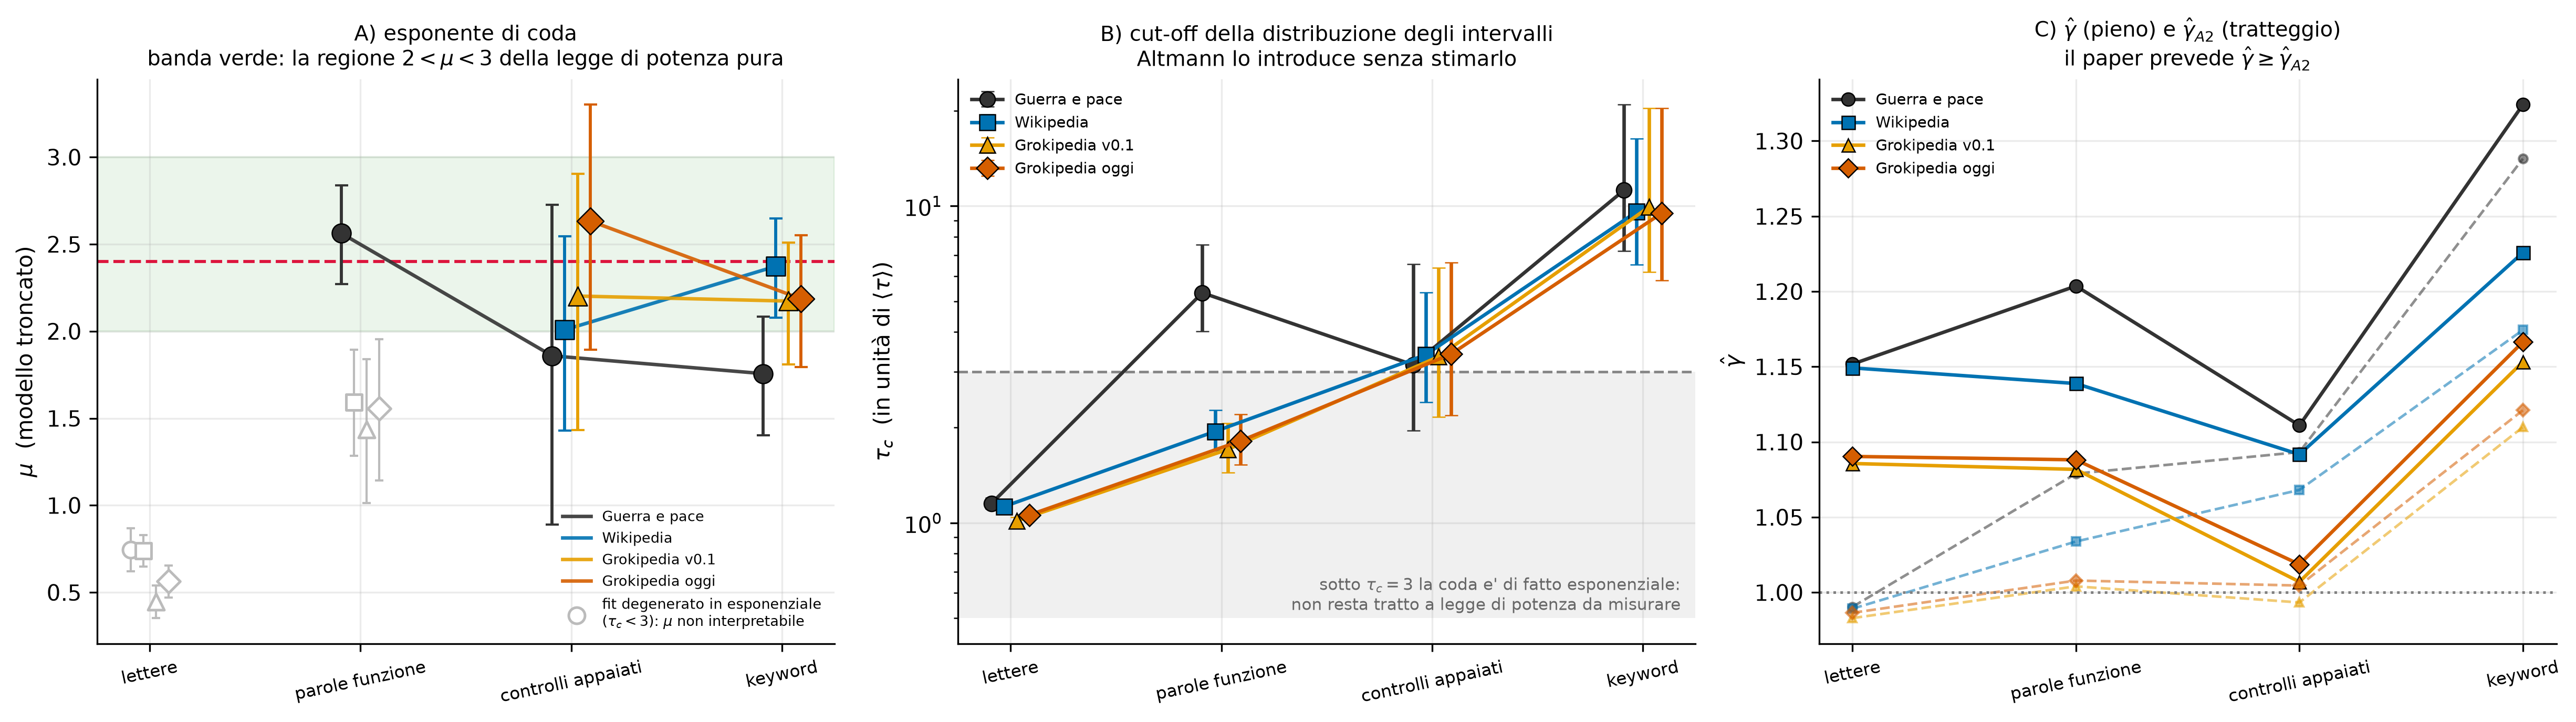
\includegraphics[width=\textwidth]{figure/cap5_esponente_coda.png}
  \caption{Stima diretta della coda della distribuzione degli intervalli. A:
  esponente $\mu$ della~\eqref{eq:coda-troncata} ai quattro livelli, con
  intervalli di confidenza di profilo; la banda verde è la regione $2<\mu<3$ in
  cui è derivata la~\eqref{eq:eq8} per la legge di potenza pura, mentre sotto il
  modello troncato adottato qui i momenti restano finiti per qualunque $\mu$ e
  la banda va letta come riferimento alla letteratura; i simboli grigi sono le
  celle in cui il fit degenera in un esponenziale e $\mu$ non è interpretabile,
  che le linee di collegamento saltano. B: cut-off
  $\tau_c$ agli stessi livelli, in unità dell'intervallo medio e con intervalli
  di confidenza di profilo; sotto la soglia tratteggiata non resta tratto a legge
  di potenza da misurare. C: $\hat\gamma$ (pieno) contro $\hat\gamma_{A2}$
  (tratteggiato) ai quattro livelli. La~\eqref{eq:disug1} è rispettata in tutte
  le celle: la curva piena sta sempre sopra la tratteggiata.}
  \label{fig:coda}
\end{figure}

\paragraph{Perché $\mu$ non serve a confrontare i corpora.}
I quattro valori non vanno però usati per ordinare i corpora, e la
Figura~\ref{fig:verosimiglianza} mostra perché: $\mu$ e $\tau_c$ sono
fortemente correlati, cosicché le regioni di confidenza congiunte sono creste
allungate anziché ellissi compatte e quelle dei tre corpora enciclopedici si
sovrappongono quasi interamente. A ciò si aggiunge la dipendenza dal punto in
cui si decide che la coda cominci: spostando $x_{\min}$ dal settantacinquesimo
al novantacinquesimo percentile $\mu$ passa da $1.65$ a $2.63$ su Wikipedia, una
variazione maggiore di ogni differenza fra corpora, e le curve si incrociano.

Di questa analisi non resta perciò un ordinamento fra corpora. Restano due
risultati, entrambi insensibili alla posizione esatta lungo la cresta: la legge
di potenza pura è rifiutata ovunque, e il cut-off cresce in modo ordinato
salendo nella gerarchia linguistica. Il cut-off è previsto
da~\cite{altmann2012} come conseguenza della discesa lungo quella stessa
gerarchia, e la sua esistenza è qui verificata invece che assunta.

\begin{figure}[htbp]
  \centering
  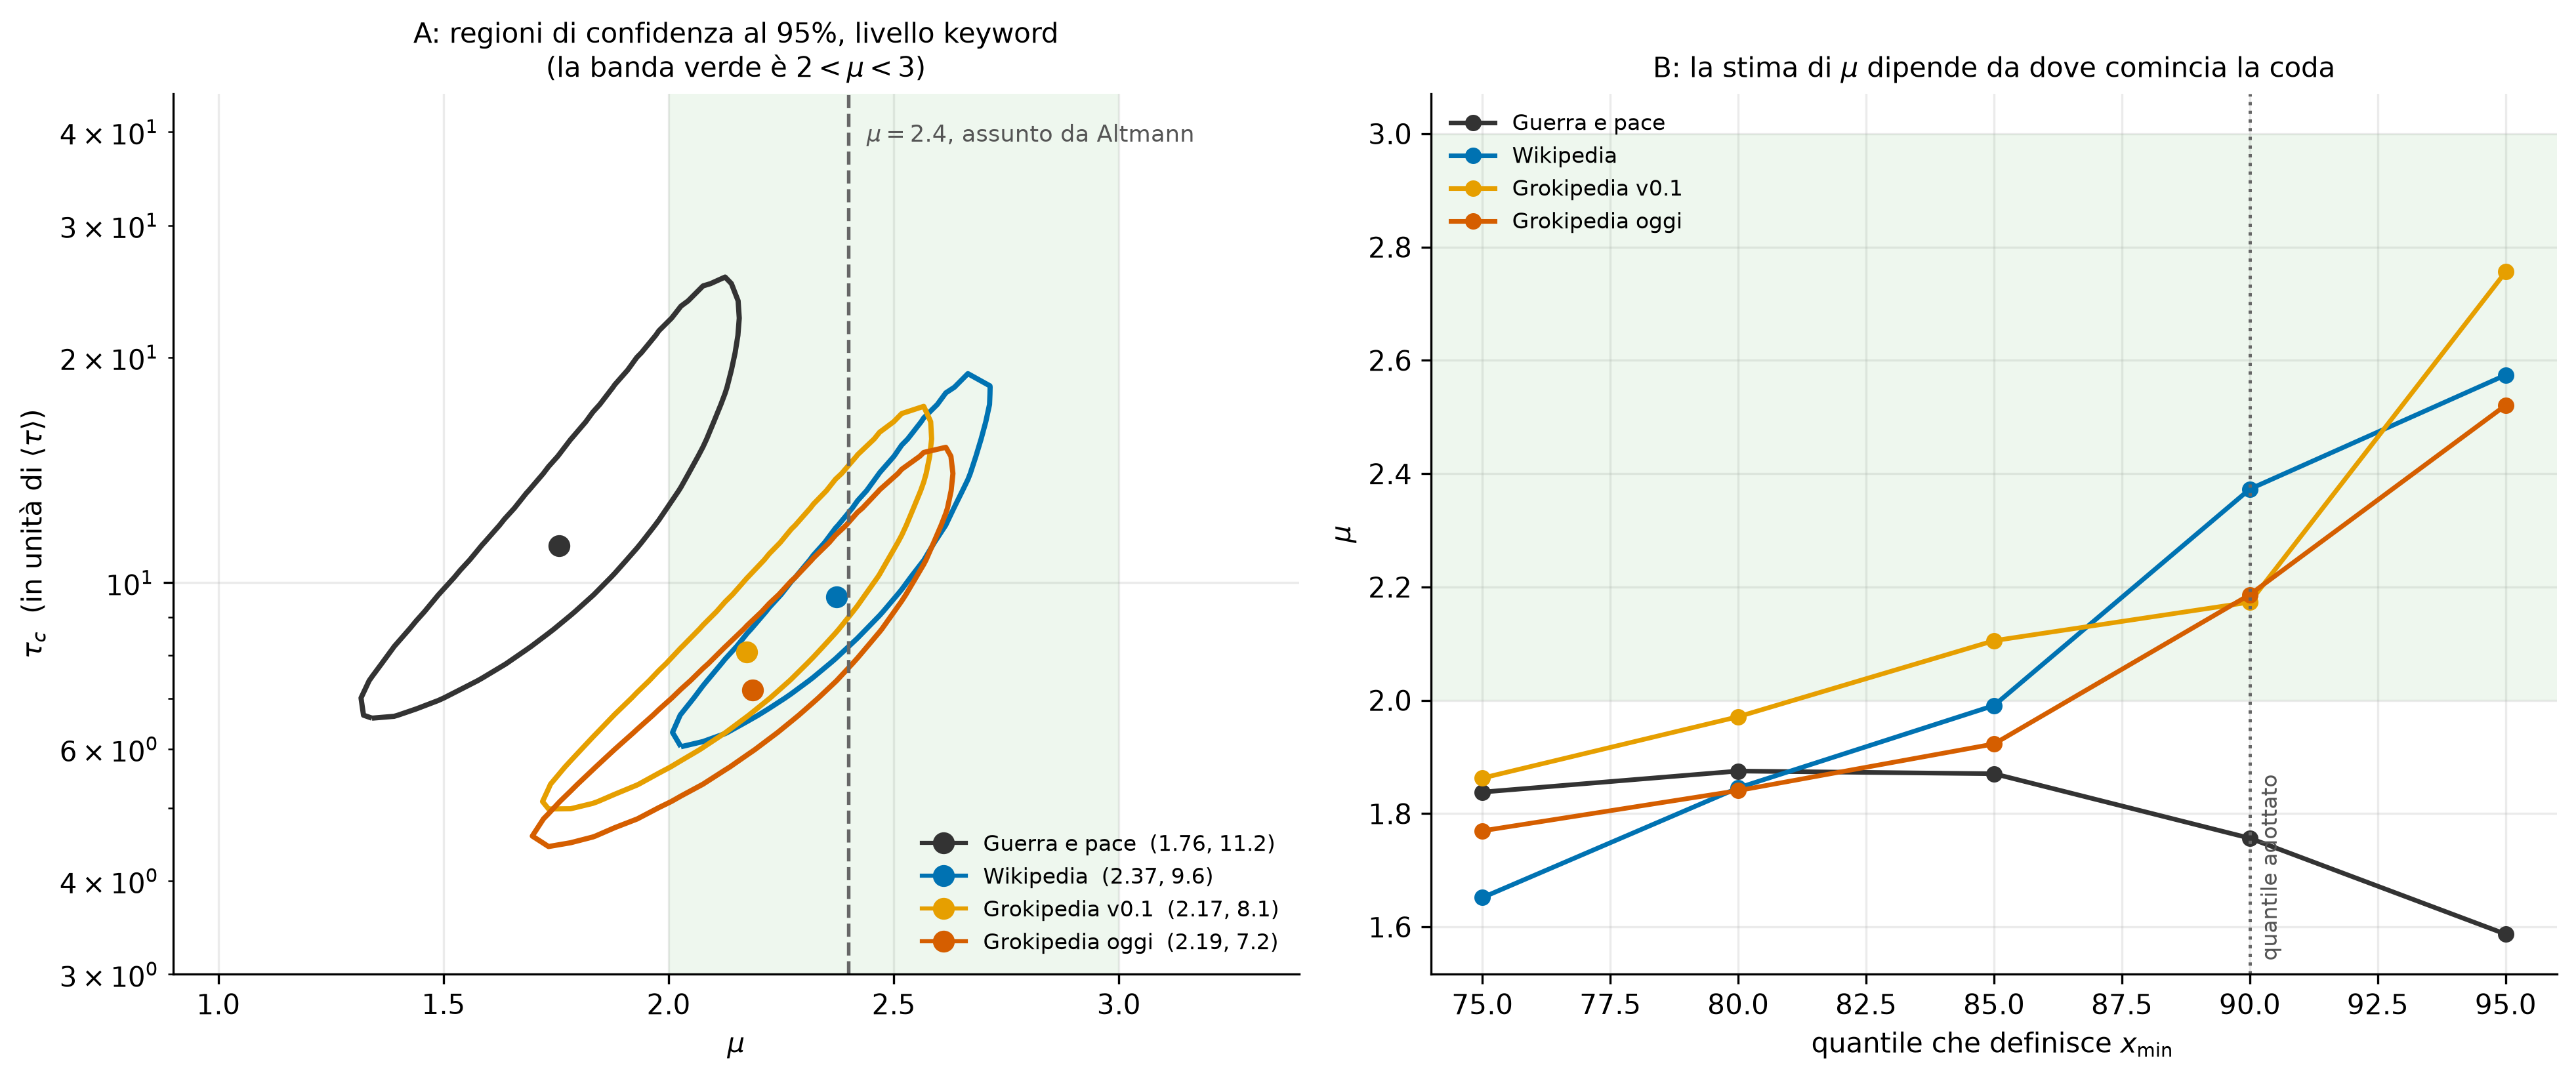
\includegraphics[width=\textwidth]{figure/cap5_verosimiglianza_coda.png}
  \caption{Perché l'esponente di coda non discrimina fra i corpora. A: regioni
  di confidenza congiunte al $95\%$ nel piano $(\mu, \tau_c)$ sul livello delle
  parole chiave, con $x_{\min}$ al novantesimo percentile; l'allungamento delle
  regioni è la correlazione fra i due parametri, e la linea tratteggiata è il
  valore $\mu = 2.4$ assunto in~\cite{altmann2012}. B: stima di $\mu$ al variare
  del quantile che definisce $x_{\min}$; le quattro curve si incrociano, cosicché
  l'ordinamento fra corpora dipende da quella scelta.}
  \label{fig:verosimiglianza}
\end{figure}

\paragraph{Il cut-off e la finestra di osservazione.} Il secondo pannello
della Figura~\ref{fig:coda} riporta $\tau_c$ ai quattro livelli, con
intervalli di confidenza di profilo. È l'altra metà di ciò
che~\cite{altmann2012} introduce senza stimare: il cut-off vi compare come
conseguenza necessaria della discesa nella gerarchia, ma non gli viene mai
assegnato un valore. Cresce in modo ordinato salendo nella gerarchia: circa
$1.1$ volte l'intervallo medio sulle lettere, dove la coda è di fatto già
esponenziale, $3.2$--$3.4$ sui controlli appaiati e $9.5$--$11.2$ sulle parole
chiave. La separazione fra i due livelli superiori è netta. Fra i quattro
corpora, invece, gli intervalli di confidenza si sovrappongono ampiamente:
neppure il cut-off ordina i corpora, e la sola cella in cui la separazione è
significativa è quella delle parole funzione del romanzo, discussa sopra.

Anche $\tau_c$ va poi letto come descrittore relativo alla lunghezza di analisi.
Ripetendo la stima sul romanzo a lunghezze crescenti, da \num{30000} a
\num{480000} caratteri, $\tau_c$ passa da $13.5$ a $94.7$: un fattore sette a
fronte di un fattore sedici sulla finestra, con un andamento non monotono che
scende prima di risalire. Il taglio non è dunque un puro artefatto, perché non
scala proporzionalmente alla finestra, ma non è nemmeno una lunghezza intrinseca
del testo. Sulla stessa serie $\mu$ si stabilizza attorno a $2.0$ alle finestre
maggiori, contro l'$1.76$ misurato alla lunghezza di lavoro: entrambi i
parametri descrivono la coda \emph{a quella lunghezza}, coerentemente con la
regola del §\ref{sec:lunghezza}.

\paragraph{Lo stimatore di Hill.} Dà sistematicamente valori più alti, $2.49$ sul
romanzo contro $1.76$ e circa $3.0$ sugli altri tre corpora contro
$2.2$--$2.4$, perché assume una legge di potenza pura su tutta la coda.
L'assenza di un plateau nel suo grafico diagnostico è ciò che ha motivato
l'adozione del modello troncato, e i suoi valori sono riportati solo a quel
titolo.

% ---------------------------------------------------------------------
\section{Entropia degli intervalli}
\label{sec:entropia-intervalli}

L'effetto di scala dichiarato nel §\ref{sec:appaiato} richiede una misura che
non risenta della lunghezza media delle frasi. È la ragione per cui il
§\ref{sec:entropia-intervalli-def} ha introdotto l'entropia degli intervalli
$J$ della~\eqref{eq:entropia-intervalli}: il logaritmo la rende invariante per
dilatazione dell'asse, cosicché frasi mediamente più lunghe non la spostano, e
la sottrazione del termine poissoniano ne cancella il bias. La grandezza è
risultata calcolabile su \num{5343} sequenze su \num{5617}, il $95\%$ del
totale.

\paragraph{Perché la misura è legittima.}
Trattandosi di una grandezza introdotta qui, la sua adozione va giustificata su
quello che fa e non su un precedente. I due ingredienti sono però entrambi
standard: l'entropia differenziale stimata per spaziature d'ordine è lo
stimatore di~\cite{vasicek1976}, e il confronto di una statistica osservata con
il valore che essa assume su un processo di Poisson di pari intensità è la
costruzione con cui in letteratura si misura la regolarità di una sequenza di
eventi, la stessa su cui poggiano la~\eqref{eq:cv} e il coefficiente
di~\cite{goh2008} usati nel resto del capitolo. Ciò che $J$ aggiunge è
l'invarianza per dilatazione, che nessuna delle due possiede e che serve qui per
una ragione specifica. Il §\ref{sec:entropia-intervalli-def} argomenta perché
debba funzionare; la validazione empirica è alla fine di questa sezione, dove la
stessa parola misurata a lunghezze diverse sposta il coefficiente di variazione
di un fattore tre e $J$ di due decimi di bit.

\paragraph{Che cosa riportano i tre pannelli.}
Il primo pannello della Figura~\ref{fig:entropia} mostra il rapporto fra $J$ e
il coefficiente di variazione sulle parole chiave. Le due misure sono
correlate, come atteso, ma la relazione non è biunivoca: a parità di
coefficiente di variazione i punti dei diversi corpora occupano fasce di $J$
diverse, il che è precisamente ciò che rende utile la seconda misura.

Il secondo pannello riporta $J$ ai quattro livelli. Sulle lettere i quattro
corpora coincidono attorno a $-0.20$, e sulle parole funzione i tre corpora
enciclopedici scendono insieme attorno a $-0.29$, con il romanzo che resta a
$-0.19$: valori negativi indicano intervalli più regolari di un
processo di Poisson. Sui due livelli superiori i corpora si separano, e sulle
parole chiave i corpora umani stanno sopra il valore poissoniano e quelli
generati vi si appoggiano: $J$ vale $+0.061$ sul romanzo e $+0.092$ su
Wikipedia, contro $-0.001$ su Grokipedia v0.1 e $-0.011$ sulla versione
attuale, questi ultimi due indistinguibili da zero. Le due enciclopedie generate
si collocano dunque sul valore poissoniano, mentre quella umana ne sta sopra:
gli intervalli fra parole chiave di Grokipedia non sono più regolari del caso,
semplicemente non sono più \emph{bursty} di esso. Il terzo pannello riporta la
distribuzione per documento e mostra che la separazione, pur con code
sovrapposte, riguarda l'intero corpus e non alcune voci.

\paragraph{La coda inferiore è fatta di soggetti di voce.}
La coda inferiore di quel pannello merita però un controllo, perché il cambio
di segno è ciò su cui l'affermazione precedente poggia. Le sequenze con $J$
più basso sono parole chiave a pieno titolo, nomi propri e non lessico di
servizio sfuggito alla lista chiusa, ma sono quasi tutte la stessa cosa: il
soggetto della voce. Fra le venti sequenze di $J$ minore, in Grokipedia
quattordici sono il soggetto dell'articolo, e in Wikipedia diciotto:
\emph{churchill}, \emph{newton}, \emph{paris}, \emph{freud}, \emph{mandela}. È
il fenomeno del §\ref{sec:tre-corpora}, che $J$ registra come gli altri
indicatori, e non è un difetto della classificazione.

Ha però una conseguenza sul cambio di segno. Escludendo i soggetti delle voci,
$54$ sequenze su $273$ in Grokipedia e $57$ in Wikipedia, tutti e tre i
corpora enciclopedici passano sopra il valore poissoniano: $+0.175$ su
Wikipedia e $+0.070$ su Grokipedia. Il divario appaiato sopravvive, $-0.087$
bit con $p < 10^{-3}$, e con esso la conclusione del paragrafo; non sopravvive
invece la lettura per segno, perché il segno negativo di Grokipedia è prodotto
dai soggetti delle voci, che il §\ref{sec:tre-corpora} ha già mostrato essere
marcatori sintattici e non semantici. Ciò che distingue i due corpora è quanto
$J$ vale, non da che parte dello zero cade.

\paragraph{Il divario appaiato.}
I confronti appaiati confermano il divario: sulle parole chiave la differenza
mediana fra Grokipedia attuale e Wikipedia vale $-0.105$ bit e quella fra la
v0.1 e Wikipedia $-0.077$ bit, entrambe con significatività inferiore a
$10^{-3}$. Sulle lettere e sulle parole funzione, per contro, le differenze sono
positive e non significative. Poiché $J$ non risente della diversa lunghezza
delle frasi, questo risultato conferma il divario del §\ref{sec:appaiato}
senza risentire di quell'effetto, ed è il punto in cui la conclusione principale
del capitolo diventa difendibile.

\paragraph{Perché il divario è più ampio sui controlli.}
Il divario è però più ampio sui controlli appaiati, $-0.209$ bit, che sulle
parole chiave, e la ragione sta in che cosa siano quei controlli. Il controllo
di una parola chiave è la parola di frequenza più vicina fra quelle che restano
dopo aver tolto le parole chiave stesse, i nomi propri e le sei parole funzione
selezionate; poiché le parole chiave sono per costruzione le più frequenti del
loro tipo, ciò che resta a quelle frequenze è in larga parte lessico di
servizio. I controlli più ricorrenti sono infatti \emph{by}, \emph{from},
\emph{with} e \emph{as} in Wikipedia, e \emph{like}, \emph{but}, \emph{that} e
\emph{this} in Grokipedia. È il livello in cui il testo generato si distingue di
più: le sue parole di servizio sono distribuite quasi uniformemente,
$J = -0.165$, mentre quelle di Wikipedia conservano un residuo di
addensamento, $J = +0.053$.

\paragraph{Composizione e stile, in parti quasi uguali.}
Le due liste di controlli sono però diverse fra loro, e la differenza potrebbe
misurare quali parole vengono selezionate anziché come sono distribuite. Le due
cause si separano restringendo il confronto alle parole che compaiono fra i
controlli di entrambi i corpora. Sono ventisei, e dodici raggiungono almeno tre
voci per corpus. Su queste il divario resta: la differenza mediana di $J$ vale
$-0.091$ bit con $p = 0.043$, e le quattro parole più spostate sono
\emph{with} ($-0.060$ contro $-0.414$), \emph{as} ($+0.227$ contro $-0.106$),
\emph{this} ($-0.005$ contro $-0.301$) e \emph{from} ($+0.057$ contro $-0.225$).
Il divario fra le medie dei due corpora, $-0.218$ bit, si scompone dunque in
$-0.128$ attribuibili alla distribuzione delle stesse parole e $-0.091$ alla
diversa composizione delle due liste, cioè in parti quasi uguali. Il valore
differisce di un centesimo dal $-0.209$ citato sopra perché quello è la mediana
delle differenze voce per voce e questo la differenza fra le medie.

La parte attribuibile alla composizione ha un contenuto proprio. I controlli di
Wikipedia sono preposizioni e ausiliari legati alla struttura del periodo, come
\emph{by}, \emph{was}, \emph{with} e \emph{for}; quelli di Grokipedia sono in
prevalenza connettivi di discorso, come \emph{like}, \emph{but}, \emph{that} e
\emph{over}. La parte attribuibile alla distribuzione descrive invece un
meccanismo: in Wikipedia una preposizione come \emph{from} si addensa dove il
contenuto la richiede, in una sezione biografica più che in una tecnica, e i suoi
intervalli ereditano il ritmo delle sezioni; in Grokipedia la stessa parola
ricorre a cadenza quasi costante lungo tutto l'articolo. Il segno negativo di $J$
dice che quella cadenza è più regolare di quella di un processo casuale, non
soltanto meno addensata.

Una verifica interna conferma la lettura. Nei controlli di Wikipedia il $93\%$
delle parole appartiene alla lista chiusa e dà $J = +0.043$, mentre il restante
$7\%$ dà $+0.188$: la classe grammaticale della parola cambia il risultato. In
Grokipedia le due quote valgono $-0.151$ e $-0.182$, indistinguibili fra loro.
Nel testo generato la regolarità degli intervalli non dipende da che tipo di
parola si stia guardando, ed è la stessa compressione uniforme della variabilità
lessicale che il §\ref{sec:sintesi-cap5} indica come conclusione del capitolo,
osservata al livello in cui si manifesta con più forza.

\paragraph{Stabilità rispetto alla lunghezza di analisi.}
Una validazione indipendente riguarda la dipendenza dalla lunghezza. Passando
da \num{40000} caratteri al romanzo intero, il coefficiente di variazione della
parola \emph{prince} cambia di un fattore $3.08$, mentre il suo $J$ si sposta di
$0.21$ bit; per la parola \emph{pierre} il coefficiente cambia di un fattore
$3.49$ e $J$ di $0.08$ bit. I due numeri non sono direttamente confrontabili,
perché il coefficiente di variazione è un rapporto e $J$ un logaritmo: uno
spostamento di $0.21$ bit corrisponde a un fattore $2^{0.21} = 1.16$ sulla
dispersione efficace degli intervalli, e uno di $0.08$ bit a un fattore $1.06$.
Riportate alla stessa scala, le due derive stanno nel rapporto di $2.7$ e $3.3$
in favore di $J$. La nuova misura è dunque circa tre volte più stabile rispetto
alla lunghezza di analisi di quella che sostituisce, il che ne conferma
l'utilità al di là del problema specifico per cui era stata introdotta.

\begin{figure}[htbp]
  \centering
  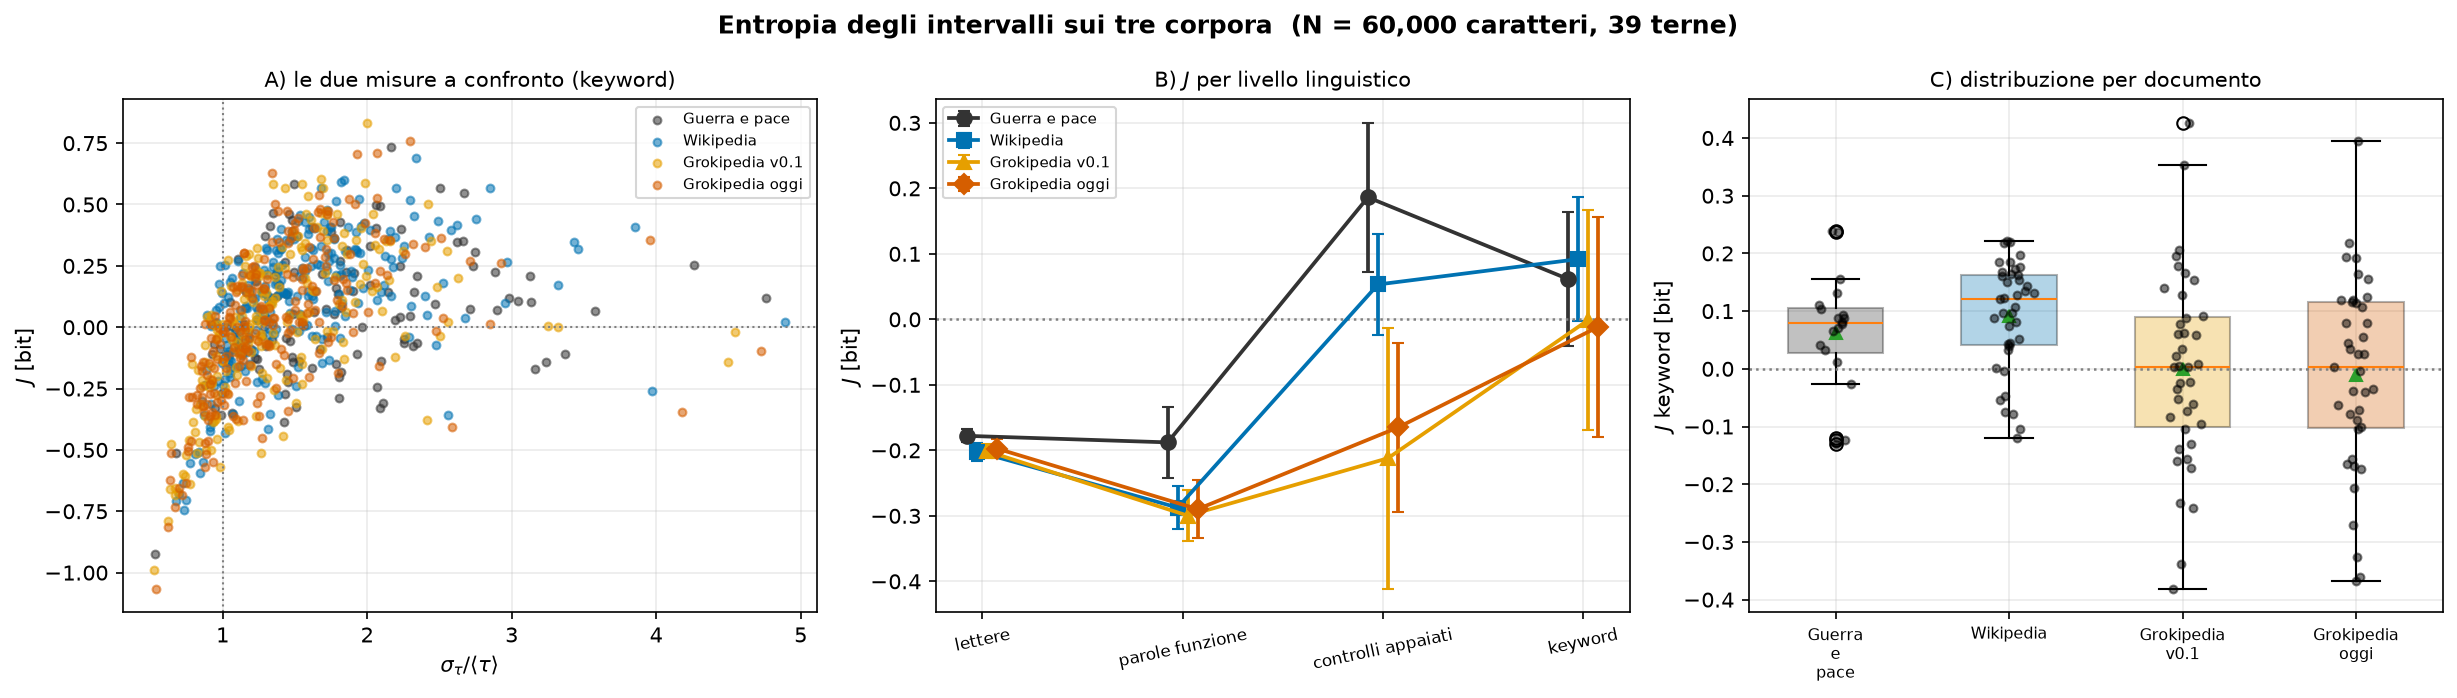
\includegraphics[width=\textwidth]{figure/cap5_entropia_intervalli.png}
  \caption{Entropia degli intervalli. A: relazione fra $J$ e coefficiente di
  variazione sulle parole chiave, un punto per sequenza. B: $J$ ai quattro
  livelli linguistici, con deviazioni standard fra testi; valori negativi
  indicano intervalli più regolari di un processo di Poisson. C: distribuzione
  di $J$ sulle parole chiave documento per documento. La misura è invariante per
  dilatazione dell'asse dei caratteri e non risente quindi della diversa
  lunghezza delle frasi nei due corpora enciclopedici.}
  \label{fig:entropia}
\end{figure}

% ---------------------------------------------------------------------
\section{Quanto pesa la definizione dei livelli lessicali}
\label{sec:effetto-stoplist}

Il paragrafo \emph{Come vengono separati i livelli lessicali} del
§\ref{sec:scelte} ha documentato l'estensione della lista chiusa di parole funzione da
\num{133} a \num{215} voci e la ragione per cui era necessaria. Questa sezione
riporta di quanto si spostano i risultati, perché lo spostamento non è
trascurabile e la scelta deve restare verificabile.

Il pannello A della Figura~\ref{fig:effetto-stoplist} riporta quali parole la
lista originaria lasciava passare fra le parole chiave di Grokipedia, e in
quante voci ciascuna: nell'elenco corrispondente di Wikipedia non ne compare
nessuna, e le sue sette parole sono distinte fra loro, ciascuna in una sola
voce.

\begin{table}[htbp]
  \centering
  \begin{tabular}{lcccc}
    \toprule
    & \multicolumn{2}{c}{lista originaria} & \multicolumn{2}{c}{lista estesa} \\
    \cmidrule(lr){2-3}\cmidrule(lr){4-5}
    & Wikipedia & Grok. oggi & Wikipedia & Grok. oggi \\
    \midrule
    keyword più bursty del controllo & $0.685$ & $0.630$ & $0.692$ & $0.740$ \\
    idem, su $\hat\gamma$ & $0.736$ & $0.663$ & $0.747$ & $0.791$ \\
    $\sigma_\tau/\langle\tau\rangle$ keyword & $1.530$ & $1.289$ & $1.536$ & $1.379$ \\
    divario appaiato, keyword & \multicolumn{2}{c}{$-0.230$} & \multicolumn{2}{c}{$-0.167$} \\
    divario appaiato, controlli & \multicolumn{2}{c}{$-0.122$} & \multicolumn{2}{c}{$-0.157$} \\
    $J$ keyword & $+0.086$ & $-0.069$ & $+0.092$ & $-0.011$ \\
    $\mu$ keyword & $2.38$ & $2.52$ & $2.37$ & $2.19$ \\
    quadrante basso-sinistra & $5.1\%$ & $24.5\%$ & $5.1\%$ & $14.3\%$ \\
    \bottomrule
  \end{tabular}
  \caption{Effetto della definizione dei livelli lessicali sui risultati del
  capitolo. Le righe dei divari appaiati riportano un solo valore perché
  misurano la differenza fra i due corpora. Le lettere e le parole funzione non
  compaiono perché nessuna parola cambia livello a quelle altezze: i loro valori
  coincidono a tutte le cifre riportate nel capitolo.}
  \label{tab:effetto-stoplist}
\end{table}

La Tabella~\ref{tab:effetto-stoplist} riporta il confronto. Tre risultati
cambiano in modo sostanziale. Il primo è il test interno: con la lista
originaria Grokipedia sembrava battere il proprio controllo appaiato meno spesso
di Wikipedia, e l'ordinamento fra i corpora appariva netto; con la lista estesa
l'ordine si inverte, e la differenza fra le due enciclopedie sparisce. Il
pannello B della figura mostra i due esiti sovrapposti. Il secondo è l'entropia
degli intervalli, il cui valore sulle parole chiave passa da $-0.069$ a
$-0.011$, cioè da un cambio di segno netto a uno indistinguibile da zero. Il
terzo è l'esponente di coda, che su Grokipedia scende da $2.52$ a $2.19$,
avvicinandosi a quello di Wikipedia anziché allontanarsene.

Restano invece stabili il divario appaiato complessivo, che si riduce da
$-0.230$ a $-0.167$ senza perdere significatività, il coefficiente di variazione
delle parole chiave, e l'intera decomposizione della~\eqref{eq:eq4}. Non si
muovono di una cifra, come è ovvio, i livelli delle lettere e delle parole
funzione.

La lezione metodologica vale al di là di questo caso. La distinzione fra
parole di contenuto e parole di servizio è la premessa dell'intero protocollo
di~\cite{altmann2012}, e viene qui operata da una lista chiusa che il paper
non specifica. Quando i corpora confrontati hanno abitudini lessicali diverse,
e un modello linguistico ne ha rispetto a un redattore umano, una lista
incompleta non introduce un rumore simmetrico: sposta sistematicamente in un
solo corpus il confine fra i due livelli, e produce un divario che non c'è.

\begin{figure}[htbp]
  \centering
  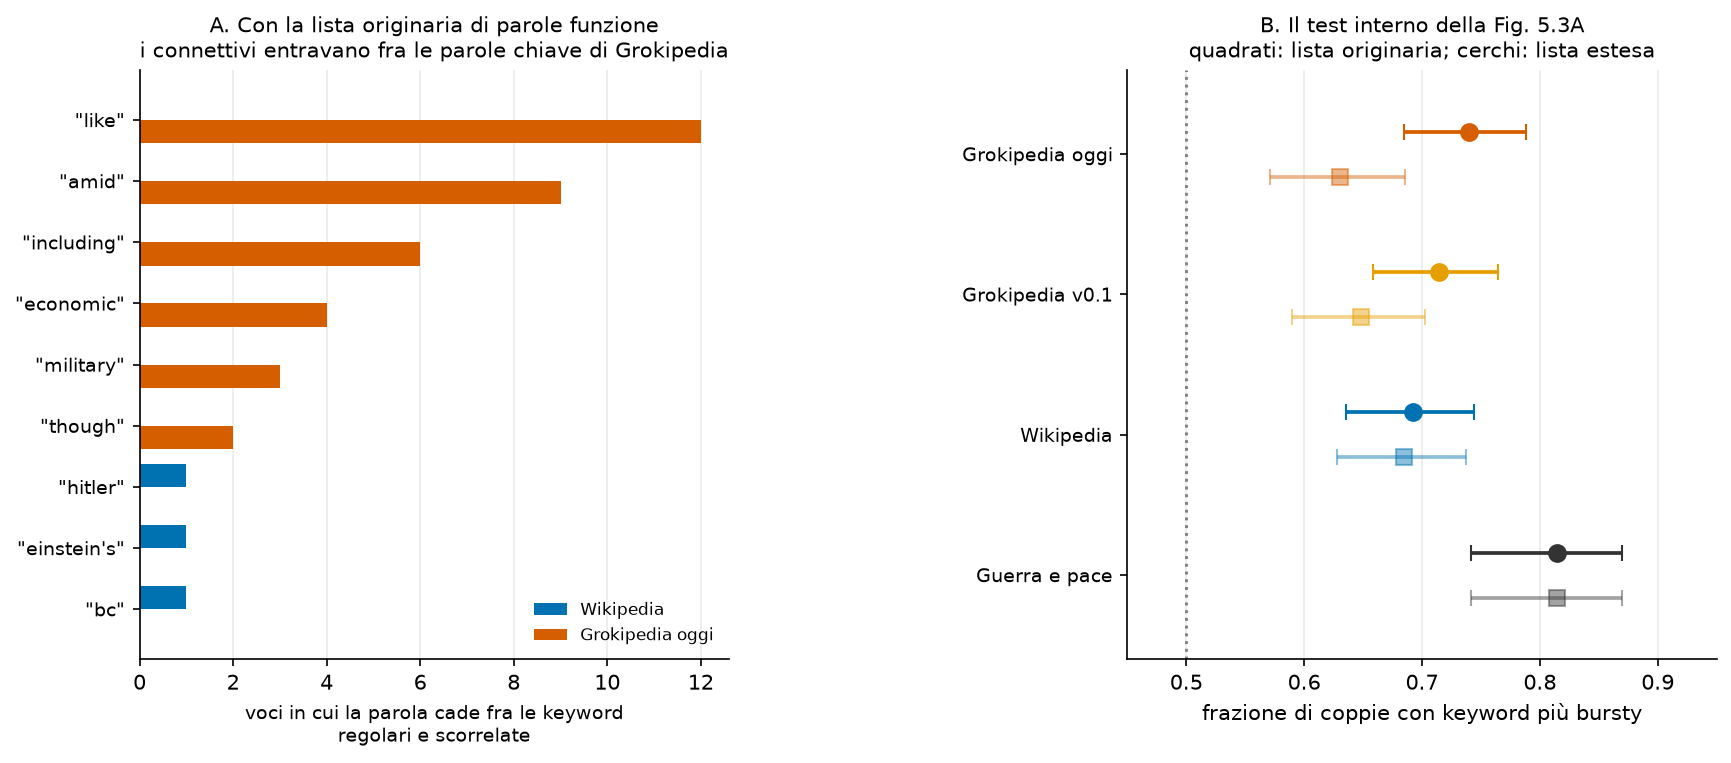
\includegraphics[width=\textwidth]{figure/cap5_effetto_stoplist.png}
  \caption{Effetto della definizione dei livelli lessicali. A: con la lista di
  funtori originaria, quali parole cadevano fra le parole chiave classificate
  come regolari e scorrelate, contate come numero di voci in cui ciò accadeva;
  le prime tre di Grokipedia sono connettivi, e in Wikipedia non compaiono. B:
  il test interno della Figura~\ref{fig:tre-corpora}A con le due
  classificazioni, quadrati per la lista originaria e cerchi per quella estesa,
  con intervalli di confidenza al $95\%$.}
  \label{fig:effetto-stoplist}
\end{figure}

% ---------------------------------------------------------------------
\section{Che cosa il testo generato non riproduce}
\label{sec:sintesi-cap5}

Il testo generato possiede correlazioni a lungo raggio, e ai livelli bassi della
gerarchia linguistica le possiede quasi nella stessa misura del testo umano:
sulle lettere i quattro corpora sono indistinguibili per coefficiente di
variazione, per entropia degli intervalli e per quota di burstiness, e sulle
parole funzione la differenza è piccola, benché significativa. Al livello delle parole il divario si apre, e vale più di un ordine
di grandezza rispetto a quello misurato sui caratteri.

Il divario non distingue però le parole che portano il contenuto dai controlli a
frequenza appaiata. I due valori sono quasi uguali alla lunghezza di lavoro,
$-0.157$ e $-0.167$, e si invertono a quella di controllo
(§\ref{sec:robustezza-neff}); e il test che chiede se la parola chiave superi il
proprio controllo \emph{dentro lo stesso testo} dà a Grokipedia un esito pari a
quello di Wikipedia, anzi lievemente migliore. Il meccanismo descritto
in~\cite{altmann2012} è dunque presente nel testo generato, e con la stessa
efficacia: ciò che manca è l'ampiezza con cui le parole, di contenuto e non, si
addensano.

Non si tratta dunque di una persistenza tematica assente, perché la distinzione
fra parole tematiche e parole ordinarie il modello la produce; si tratta di una
compressione uniforme della variabilità lessicale, che riduce la burstiness di
tutte le parole senza alterare il rapporto fra le une e le altre. Vale ancora la
distinzione posta nel §\ref{sec:intro-linguaggio} fra riprodurre le proprietà
statistiche del linguaggio e riprodurre il meccanismo che le genera, ma
applicata a un livello più basso di quanto la prima lettura suggerisse.

Ciò che il capitolo misura è la distanza fra due enciclopedie appaiate titolo
per titolo, e null'altro. Il deficit è osservato su Grokipedia, cioè su un unico
sistema generativo, in un unico dominio e in una sola lingua: nulla di quanto
riportato qui stabilisce che sia una proprietà dei modelli linguistici in
generale anziché di quel sistema. Il Capitolo~\ref{cap:risultati1} non offre un
appoggio indipendente su questo punto: misura un altro corpus, con grandezze
che non arrivano al livello a cui il divario si manifesta.
